\documentclass[12pt]{article}

% USEPACKAGES
\usepackage[table]{xcolor}
\usepackage[margin=2.5cm]{geometry} % Change border margins.
\usepackage[titles]{tocloft} % Table of Contents, manual add.
\usepackage{mcode} % Load matlab code into LaTeX.
\usepackage[parfill]{parskip} % Removes indents
\usepackage[hidelinks]{hyperref} % Clickable links in PDF.
\usepackage{fancyhdr}
\usepackage{graphicx}
\usepackage{epstopdf}
\usepackage{float}
\usepackage{amsmath,amssymb,amsthm,multirow,algorithm,algorithmic,amsfonts}
\usepackage{gensymb}
\usepackage[square,numbers,comma,sort&compress]{natbib}
\usepackage[titletoc]{appendix}
\usepackage[final]{pdfpages}
\usepackage{afterpage}
\usepackage{mdwlist} % Compact lists (itemize*)
\usepackage{fixltx2e}
\usepackage{expl3}
\usepackage{datatool}
\usepackage[nogroupskip,acronyms,symbols]{glossaries}
\usepackage{glossary-longragged}
\usepackage{wrapfig}
\usepackage{caption}
\usepackage{multicol}
\usepackage{subcaption}
\usepackage{pgfplots}

\usepackage{lscape}
\usepackage{rotating}
\usepackage{pdflscape}

\usepackage{titlesec}

\usepackage{pifont}

\usepackage{array}

\newcolumntype{C}[1]{>{\centering\arraybackslash}p{#1}}

%\usepackage{setspace}

\newcommand{\cmark}{\ding{51}}%
\newcommand{\xmark}{\ding{55}}%

\newlength\figureheight 
\newlength\figurewidth
\pgfplotsset{compat=1.3}

% PAGESTYLE
\pagestyle{plain}

% Generate the glossary
	% create a new glossary style for the list of symbols
	% copied (but eddited) from http://www.latex-community.org/forum/viewtopic.php?f=5&t=20797
	\newglossarystyle{listos}{%
	  \glossarystyle{altlongragged4col}
	  \setlength{\glsdescwidth}{0.8\textwidth}
	  % allow line wrap in the description column
	  \renewenvironment{theglossary}%
		    {\begin{longtable}{llp{\glsdescwidth}}}%
		    {\end{longtable}}%
		  \renewcommand{\glsgroupskip}{}% make nothing happen between groups
		  \renewcommand*{\glossaryheader}{%
		  \bfseries Symbol & \bfseries Unit & \bfseries Description \\\endhead}%
		  % No heading between groups:
		  \renewcommand*{\glsgroupheading}[1]{}%
		  % Main (level 0) entries displayed in a row optionally numbered:
		  \renewcommand*{\glossentry}[2]{%
		  \glsentryitem{##1}% Entry number if required
		  \glstarget{##1}{\glossentryname{##1}}% Name
			& \glossentrysymbol{##2}% Unit
			& \glossentrydesc{##2}% Description
			\tabularnewline % end of row
		  }%
		  % Similarly for sub-entries (no sub-entry numbers):
		  \renewcommand*{\subglossentry}[3]{%
		  % ignoring first argument (sub-level)
		  \glstarget{##2}{\glossentryname{##2}}% Name
			& \glossentrysymbol{##2}% Unit
			& \glossentrydesc{##2}% Description
			\tabularnewline % end of row
			}%
			% Nothing between groups:
			\renewcommand*{\glsgroupskip}{}%
			}
	
	% create a new glossary style for the list of constants
		% copied (but eddited) from http://www.latex-community.org/forum/viewtopic.php?f=5&t=20797
		\newglossarystyle{listoc}{%
		  \glossarystyle{altlongragged4col}
		  \setlength{\glsdescwidth}{0.8\textwidth}
		  % allow line wrap in the description column
		  \renewenvironment{theglossary}%
		    {\begin{longtable}{lllp{\glsdescwidth}}}%
		    {\end{longtable}}%
		  \renewcommand{\glsgroupskip}{}% make nothing happen between groups
		  \renewcommand*{\glossaryheader}{%
		  \bfseries Symbol & \bfseries Value & \bfseries Unit & \bfseries Description \\\endhead}%
		  % No heading between groups:
		  \renewcommand*{\glsgroupheading}[1]{}%
		  % Main (level 0) entries displayed in a row optionally numbered:
		  \renewcommand*{\glossentry}[2]{%
		  \glsentryitem{##1}% Entry number if required
		  \glstarget{##1}{\glossentryname{##1}}% Name
			& \glsentryuseri{##2}% Value
			& \glossentrysymbol{##2}% Unit
			& \glossentrydesc{##2}% Description
			\tabularnewline % end of row
		  }%
		  % Similarly for sub-entries (no sub-entry numbers):
		  \renewcommand*{\subglossentry}[3]{%
		  % ignoring first argument (sub-level)
		  \glstarget{##2}{\glossentryname{##2}}% Name
			& \glsentryuseri{##2}% Value
			& \glossentrysymbol{##2}% Unit
			& \glossentrydesc{##2}% Description
			\tabularnewline % end of row
			}%
			% Nothing between groups:
			\renewcommand*{\glsgroupskip}{}%
			}

	
\newglossary*{symbol}{List of Symbols}
\newglossary*{constants}{List of Constants}
\makenoidxglossaries
\setacronymstyle{long-short}
\loadglsentries{./Acronyms}
\newglossaryentry{romanletter}{type=symbol,name={},description={\nopostdesc},sort=a}
\newglossaryentry{greekletter}{type=symbol,name={},description={\nopostdesc},sort=b}
\newglossaryentry{romanletterc}{type=constants,name={},description={\nopostdesc},sort=a}
\newglossaryentry{greekletterc}{type=constants,name={},description={\nopostdesc},sort=b}
\loadglsentries{./Symbols}
\loadglsentries{./Constants}



% COMMANDS
\newcommand{\HRule}{\rule{\linewidth}{0.04cm}}
\renewcommand{\abstractname}{{\Large Summary}}
\renewcommand{\cftsecleader}{\cftdotfill{\cftdotsep}}
\setlength{\parskip}{6pt plus4pt minus2pt}
\setcounter{tocdepth}{3}
% ENVIRONMENTS
\newenvironment{drawing}


% Paragrap is now an extra subsection
\setcounter{secnumdepth}{4}

\titleformat{\paragraph}
{\normalfont\normalsize\bfseries}{\theparagraph}{1em}{}
\titlespacing*{\paragraph}
{0pt}{3.25ex plus 1ex minus .2ex}{1.5ex plus .2ex}


\begin{document}
% Titlepage
\begin{titlepage}
\begin{center}

% Upper part of the page
\textsc{\LARGE Delft University of Technology}\\[0.3cm]
\textsc{\Large Design Synthesis Exercise}\\[0.5cm]

% Title
\HRule \\[0.4cm]
{\Large \bfseries Design of a Controllable Inflatable Aeroshell}\\[0.2cm]
{\Huge \bfseries Project plan}\\[0.2cm]
\HRule \\[1.2cm]

% Image
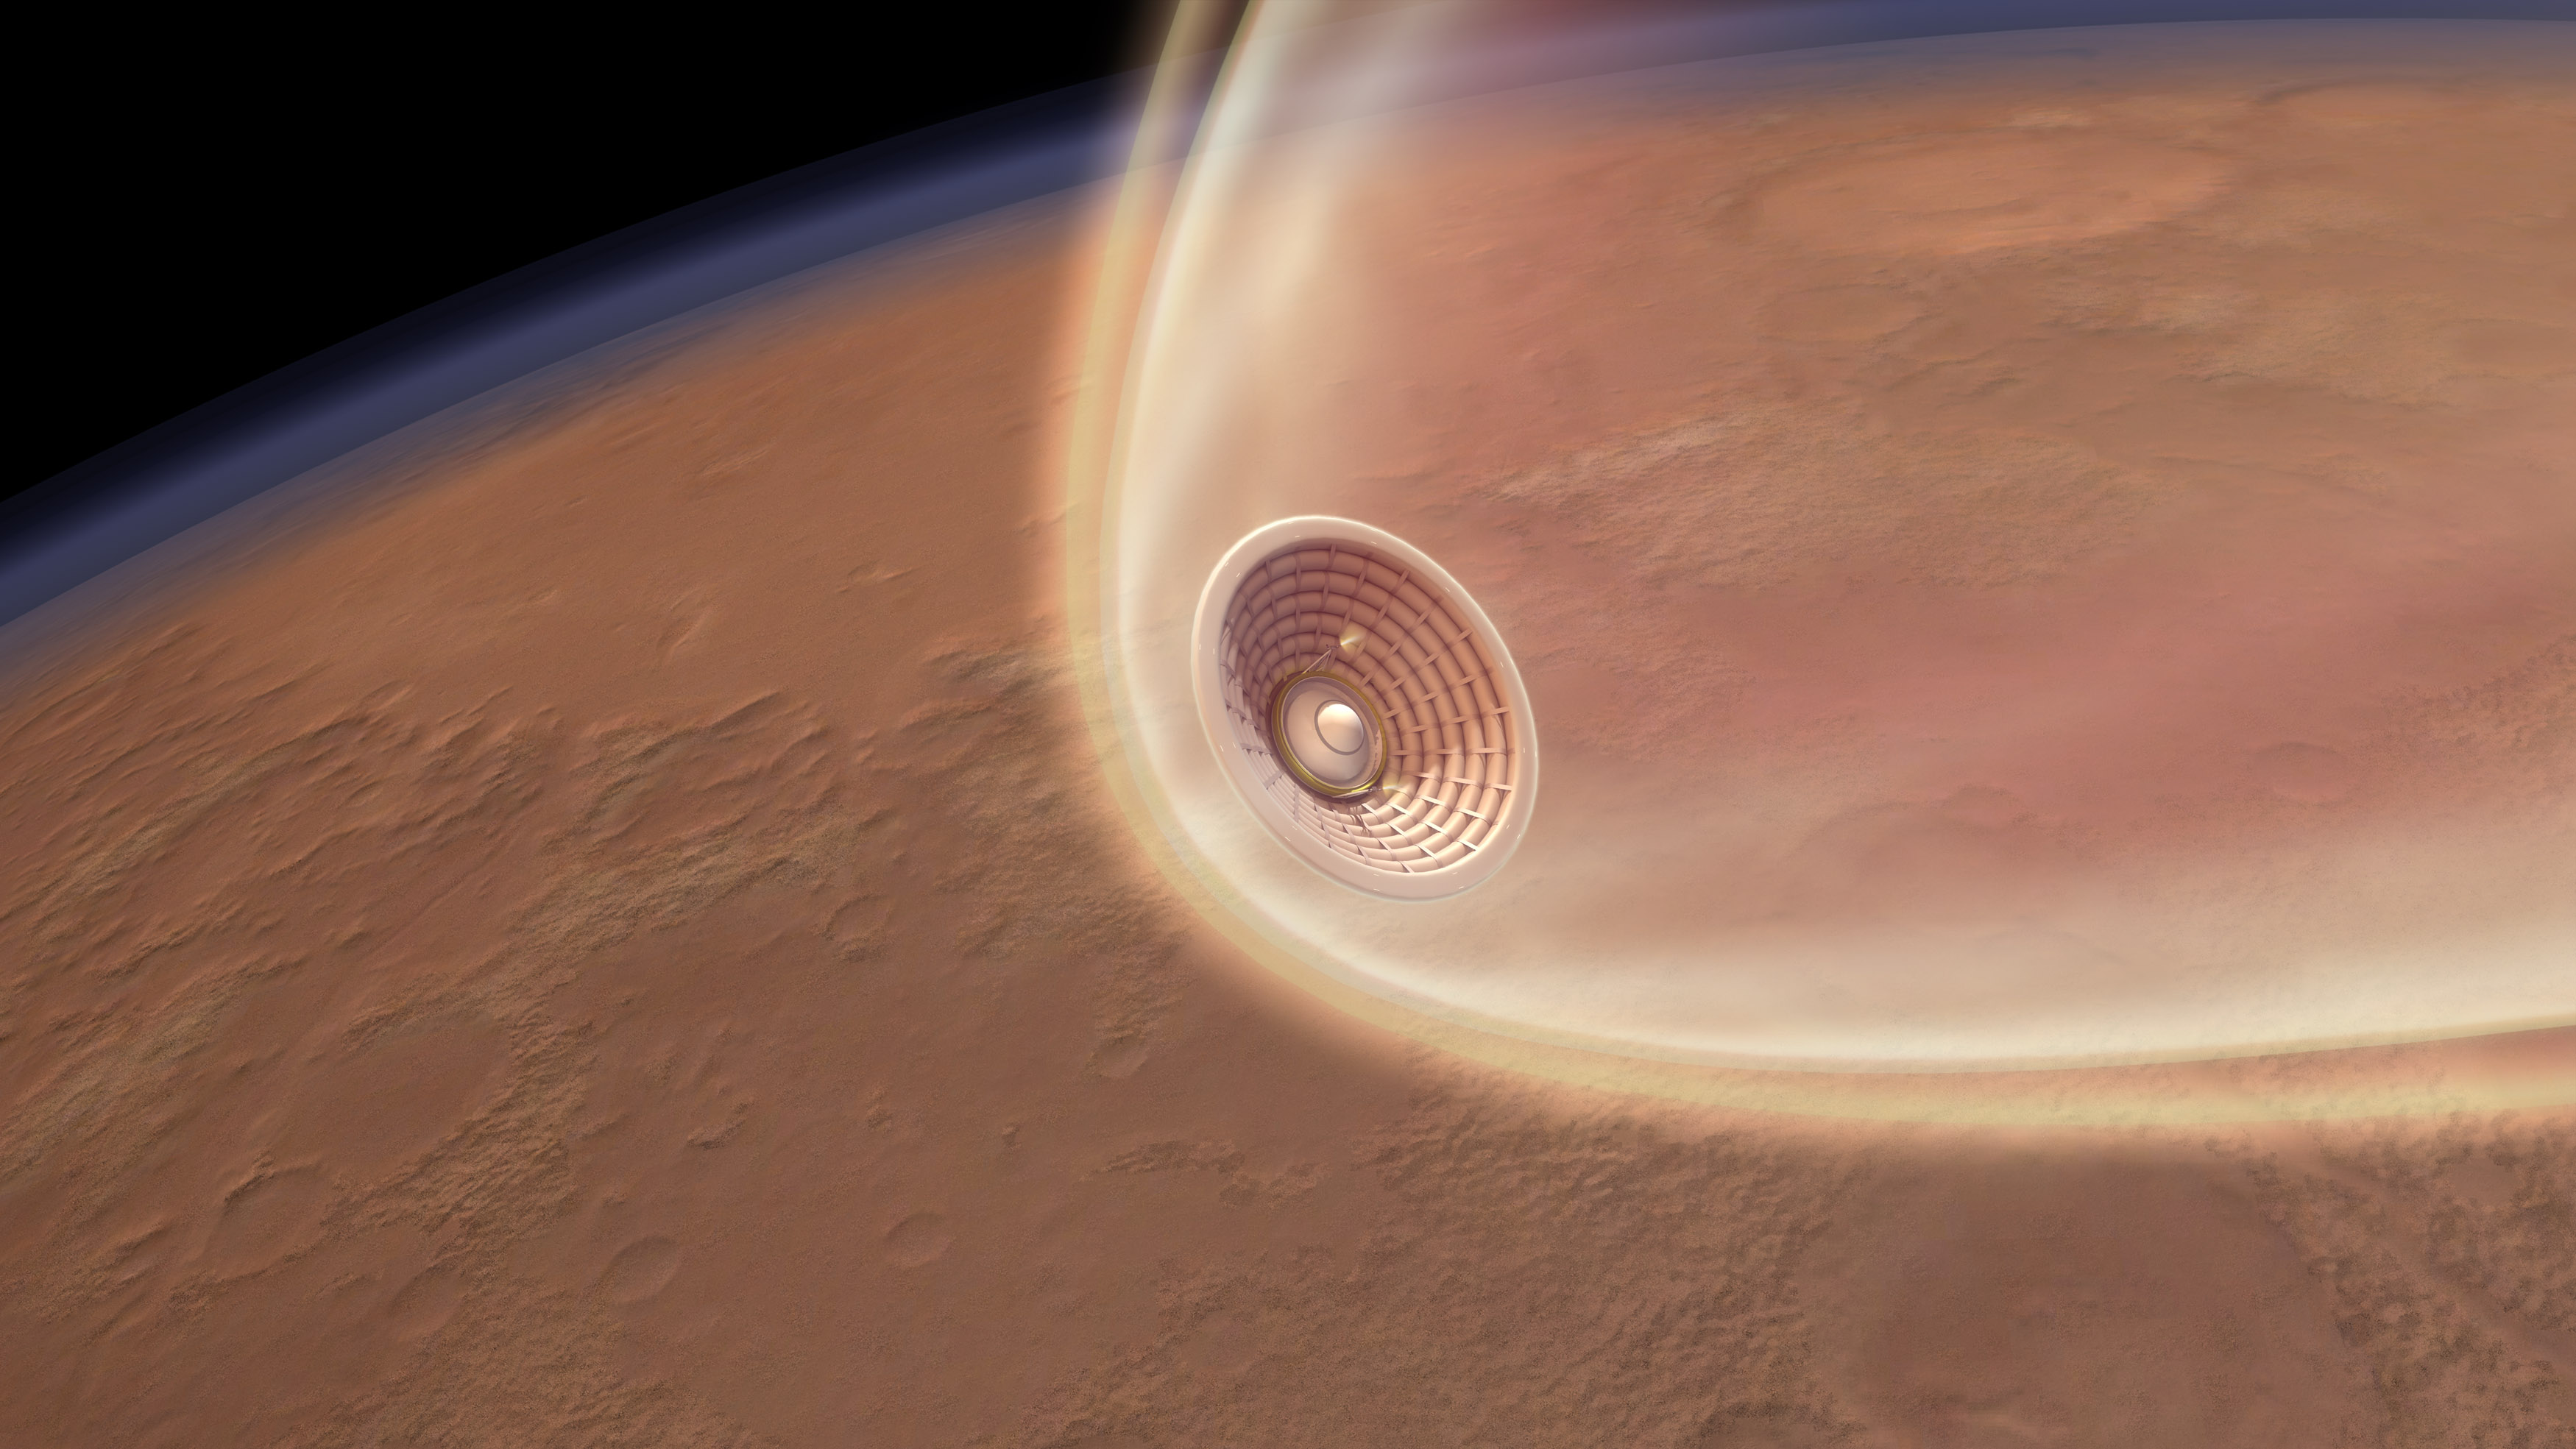
\includegraphics[scale=0.4]{./Titlepage/coverpicture}\\[1cm]

% Author
S. Balasooriyan \\
B. van Dongen \\
D.D. Hage \\
T. Keijzer \\
G. van Koppenhagen \\
L. Mathijssen \\
J. Meulenbeld \\
A. van Oostrum	\\
S. van Schie \\




\vfill

% Date
\begin{large}\today \end{large}

\end{center}
\end{titlepage}
% empthy page after titlepage
\newpage
\thispagestyle{empty}
\mbox{}
\pagenumbering{roman}
\setcounter{page}{0}
% Summary
\newpage
\section*{Preface}\label{cha:preface}

\begin{flushright}
	\today
\end{flushright}

Dear Reader,	
\\ [1cm]
A growing interest in manned spaceflight and human exploration of Mars requires a new solution. Conventional, rigid entry solutions require a significant decelerator mass to bring the payload to ground. Inflatable concepts offer significant mass and packaging advantages and their application opens up broad venues for interplanetary human spaceflight. 

This Final Report centres around the analysis and design of a \acrlong{cia} that is capable of bringing two crew members to the Martian surface with a mere $10\%$ decelerator mass fraction within 10 days. Conceptual and preliminary design have shown the feasibility of such a mission with its corresponding economical benefits and reduced ecological footprint by a decreased required number of launches through increased payload-carrying capability.

We would like to acknowledge dr. ir. H.J. Damveld, ir. D. Dolkens and ir. N. Reurings for their guidance and support. Moreover, we would like to thank all other staff members of the Delft University of Technology that have been of assistance.
%This Mid-Term Report is part of the deliverables for the \acrfull{mtr}. It describes the development, verification and validation of the computational tools produced to analyse several possible concepts for a controllable inflatable aeroshell designed for manned spaceflight. In addition to analysing these concepts a trade-off will be made between them to determine which is the most promising. This concept will then be further analysed in the coming period. The goal of this project is to develop an inflatable aeroshell system that can be used for atmospheric entry on Mars and is lighter than the current solutions to this problem.
\\ [1.5cm]
Design Synthesis Exercise Group 02

\section*{Summary}\label{cha:summary}


Inflatable aeroshell concepts hold the key to what is currently unattainable for interplanetary human spaceflight. In the wake of current \acrfull{nasa} investigations on the feasibility of inflatable decelerators for hypersonic guidable re-entry, this study focuses on Mars entry of a payload mass of at least 9000 [kg] using an inflatable aerodynamic decelerator of at most 1000 [kg]. Such a solution provides a large economical advantage over conventional solutions by maximizing payload-carrying capability through a light-weight device less burdened by launcher size considerations. This Mid-term Report gives an overview of conceptual design activities, comprising aerodynamic, structural, thermal, astrodynamic and control tool development and analysis, leading up to concept selection in a trade-off.
\newline
\newline
To aid in the conceptual analysis, design and selection process and to provide a basis for further design efforts after concept selection in the \acrfull{mtr} a number of tools have been developed with the following purposes:
\begin{itemize}
\item A tool for parametric structural mass modelling
\item A modified Newtonian flow aerodynamic tool for the characterisation of aerodynamic and aerothermal behaviour
\item A thermal model for \acrfull{tps} sizing and analysis
\item An astrodynamic tool with an implemented control system for trajectory control
\end{itemize}

Concepts were selected for trade-off as the outcome of a structured \acrfull{dot} on the basis of concept shape. Shape is chosen to have a leading factor due to its importance in the aerodynamic and trajectory performance, which directly flows down to thermal, structural and control performance. The initial concept selection yielded five concepts for trade-off: a conventional capsule concept and four inflatable concepts, namely stacked toroid, tension cone, trailing ballute and isotensoid configurations. To reflect concept capability of meeting customer demand, the following concept aspects have been evaluated as trade-off criteria: decelerator mass, development risk, vehicle stability and deceleration time.
\newline
\newline
The first trade-off criterion, decelerator mass, is essential since it is highly desirable that payload-carrying capability is maximised. To make full use of the launcher carrying capability, a decrease in decelerator mass allows for an equal increase in payload mass. To this end, structural, thermal and control system mass were estimated as the distinguishing mass components between concepts. 

The lowest structural mass was achieved by the stacked toroid configuration, followed upon closely by the isotensoid, tension cone and trailing ballute configurations (an estimated 110, 168 and 221 \% of stacked toroid structural mass respectively). \acrfull{tps} and control system mass analysis yielded estimates of 100, 84, and 76 \% and 100, 67, and 96 \% of stacked toroid mass for tension cone, trailing ballute and isotensoid configurations respectively. This yields total decelerator masses of 116, 113 and 88 \% of stacked toroid mass, based on weight contributions of 20, 50 and 15 \% by structure, \gls{tps} and control system mass. A mass analysis for the rigid concept showed a decelerator mass well in excess of the imposed maximum 1000 [kg], 2945 [kg] for thermal and structural mass alone.
\newline
\newline
The second trade-off criterion, development risk, is essential since concepts with a low \acrfull{trl} incur higher schedule and cost risks. The tried-and-true rigid solution thereby has \gls{trl} 9, while inflatable concepts are notably less explored. A recent surge in interest in inflatable concepts by \gls{nasa} and a consistent development program has brought the stacked toroid configuration to \gls{trl} 7. The other three inflatable concepts are less explored, having only undergone a selected set of tests and research and hence designated \gls{trl} 4. The trailing ballute concept is deemed to have a higher development risk still, by its only feasible control option being a relatively underdeveloped one, namely morphing, reflected by \gls{trl} 2.
\newline
\newline
The third trade-off criterion, deceleration time, is evaluated as a shorter entry time is desirable. As ground operations are to be maintained at fully capacity during entry, a shortening of entry time will alleviate costs incurred. Moreover, physical taxation of human payload is decreased as deceleration time is decreased.  A decreased deceleration time is obtained by better controlability of the spacecraft. To this end, concepts were evaluated for their performance in lift to drag ratio. The rigid concept was found to be able to provide a relatively high lift to drag ratio which consequently will result in short deceleration time. The stacked toroid, tension cone and ballute concept were found to provide an adequate value and finally the isotensoid deceleration performance was found to be poor in this trade-off criteria.
\newline
\newline
It is preferable that concepts are stable, since a stable vehicle will counteract perturbations to move back to its equilibrium condition and its intended trajectory. To this end, static stability was investigated by aerodynamic analysis. Stacked toroid, tension cone and ballute were found to be stable; the rigid concept is neutrally stable and the isotensoid is unstable. The first three therefore perform well, the rigid concept performs adequately and performance of the isotensoid is deficient for the fourth and final trade-off criterion.
\newline
\newline
On the basis of the analysis presented in this Mid-Term Report, design options and their prospective advantages and disadvantages are presented to the customer at the \gls{mtr}. Hereafter dialogue is entered to yield a final concept for preliminary design that satisfies customer demands. The next phase then commences with a more detailed analysis and design of the selected concepts, aided by tool enhancement. This phase entails a more refined orbit optimization, aerodynamic shape determination and structural and \gls{tps} design and sizing. A structured approach to this next phase is facilitated by breaking down future work, resource allocation and is aided by an interface definition given in this report to define the interaction of subsystems within the design process.


% Table of contents
\newpage
\tableofcontents
\addtocontents{toc}{\protect\contentsline {section}{Acronyms}{vi}{}}
\addtocontents{toc}{\protect\contentsline {section}{List of symbols}{vii}{}}
\addtocontents{toc}{\protect\contentsline {section}{List of Figures}{ix}{}}
\addtocontents{toc}{\protect\contentsline {section}{List of Tables}{xi}{}}

\newpage
\printnoidxglossary[type=\acronymtype,nonumberlist]
\newpage
\renewcommand{\arraystretch}{1.1}
\printnoidxglossary[type=symbol,nonumberlist,style=listos]
\printnoidxglossary[type=constants,style=listoc]
\setcounter{table}{0}
\newpage
\listoffigures
\newpage
\listoftables

% Chapters
\newpage
\pagenumbering{arabic}

\section{Introduction}
\label{cha:introduction}
Before human interplanetary spaceflight can be achieved technological gains have to be made in several fields. One of these fields comprises hypersonic deceleration systems. Significant weight gains are expected to be possible by using inflatable aeroshells. However, the development of a controllable inflatable aeroshell is very complex and consists of many different disciplines. To reduce the complexity of designing such a system first a \acrfull{pp} was made. Following that a \acrfull{br} was produced, in order to survey the current technology state and knowledge on this subject. Now a \acrfull{mtr} report is made in order to perform a concept trade-off. 

The purpose of this report is to present several concepts for a controllable inflatable aeroshell and to determine which concept is best suited for performing the design mission. First the group organisation for the period between the \acrlong{mtr} and \acrlong{fr} is discussed in chapter \ref{ch:wdd}, including individual and group tasks and work packages. A \acrfull{wbs} is made, together with a \acrfull{wfd} and Gantt chart. Secondly the approach with respect to sustainable development is presented in chapter \ref{ch:sustain}. Thirdly the \glspl{dot} are used in chapter \ref{ch:options} to generate several system concepts. These concepts will be analysed with tools from several different disciplines. These consist of an astrodynamics \& control tool, as well as tools for concept mass estimation, aerodynamical characteristics and thermodynamic behaviour. The development, verification, validation of these tools is discussed in chapters \ref{ch:astrocontrol}, \ref{ch:strucmass}, \ref{ch:aero_analysis} and \ref{ch:thermtool} respectively. These chapters also show the results obtained from analysing the proposed system concepts. After the tool development and concept analysis the risk inherent to each system concept is considered in chapter \ref{ch:riskestimation}. This will be done by making a risk map for each concept. Finally the concept trade-off will be performed in chapter \ref{ch:tradeoff}, based on results of the analyses conducted in the previous chapters. The result of this is a complete trade-off matrix, after which the customer will be able to select the preferred concept based on the weights they attach to each trade-off criterion.
\section{Mission description}\label{cha:missiondescr}

This chapter serves to provide on overview of the general mission layout. The mission outline from launch to final return is discussed in Section \ref{sec:missionoutline}. A full mission outline is provided, but the report focuses around the design of a \gls{hiad}. Ground operations are covered in Section \ref{sec:gop}. This mission scope is explained in Section \ref{sec:missionscope}. A short overview of the top level requirements is provided in Section \ref{sec:missionreq}. A market analysis, the sustainable development strategy and a cost breakdown are provided in Sections \ref{sec:marketanalysis}, \ref{sec:sustainable} and \ref{sec:costbreakdown} respectively. 

\subsection{Mission outline} \label{sec:missionoutline}
The mission outline is separated in five phases: Mission launch, interplanetary transfer, aerocapture and entry, terminal descent and return. The mission is centered on the aerocapture and entry phase. %All of these mission phases are discussed in the subsequent Sections.

\subsubsection{Launch} \label{sec:launch}
Mission launch is the first phase of the mission. Launch serves to bring the \gls{hiad} and accompanying mission elements in a transfer orbit towards Mars. From the top level requirements as summarised in \ref{sec:missionreq} an approach speed of 7 [$km\cdot s^{-1}$] is desired which is an implicit requirement on the total mission duration.
Based on this requirement specific launch operations can be considered and additional mission requirements can be considered. Important factors include payload size, loads and required velocity increments. Launch is important to consider also in the \gls{hiad} design as a lot of the requirements can be traced down to mission launch.

The launch mission phase initiates with the take-off from earth. In order to reach the Martian atmosphere with the desired approach speed a total velocity increment of about 19.6 [$km\cdot s^{-1}$] is required. This velocity increment comes forth of the escape velocity of the Earth to its sphere of influence and an additional velocity increment to reach the Martian atmosphere with the required approach velocity.

The velocity increments are typically subdivided into two parts: a first velocity increment into \gls{leo} and a second velocity increment into the transfer orbit. Within the \gls{leo} separate payload modules such as the \gls{hiad} and a possible habitation module may be joined \cite{George2009}. The period in \gls{leo} also allows for more precisely controlled arrival conditions at Mars as, to a certain extend, the launch is omitted from the timing sequence. 

The velocity increments up to \gls{leo} are typically subdivided into multiple integrated stages or launchers for optimal efficiency as no single launcher can deliver the total required velocity increment. These stages are separated after depletion of the propellant.

Important considerations concerning the launch are the encountered vibrations and loads as well as the total mass required to bring into the transfer orbit. Launch vibration should be considered as the natural frequencies of the subsystem should remain above the launch-induced vibrations. Moreover the vibrations require all components to be properly stowed. This should for example be considered for the inflatable part of the decelerator, which is stowed during launch.

Launch loads are typically in the order of 2.8-4.3 g's in longitudinal and 0.9-3 g's in lateral direction \cite{Wertz2011}, which is above the maximum allowed top level deceleration of 3g into the Martian atmosphere. For this reason launch loads are an important factor for the structural sizing of the aeroshell and accompanying elements. 

A launcher currently being developed for missions to Mars is the \acrfull{sls} developed by \gls{nasa}. The \gls{sls} features multiple stages and allows for a 5 [$m$] diameter in line with the top level mission requirements. The \gls{sls} features multiple stages able to deliver the required velocity increments. Its design takes close account of the Orion spacecraft which is being developed to, in the future, go to Mars. For the modules featuring a 5 [$m$] diameter payload the volume using this launcher is constraint to 225 [$m^3$] \cite{NASA2014}.

The launch phase is concluded with the start of the interplanetary phase after the final velocity increment in \gls{leo}. 



\subsubsection{Interplanetary transfer} \label{sec:interplanetary}
The interplanetary transfer time has a big impact on the design. The interplanetary transfer time determines for instance the mass of food for the astronauts, the amount of radiation to endure, how much they need to exercise and more. Keeping the transfer time short will minimise these problems. However it will also increase the $\Delta\gls{sym:V}$-budget needed for the launcher. 

\begin{figure}[h]
	\centering
	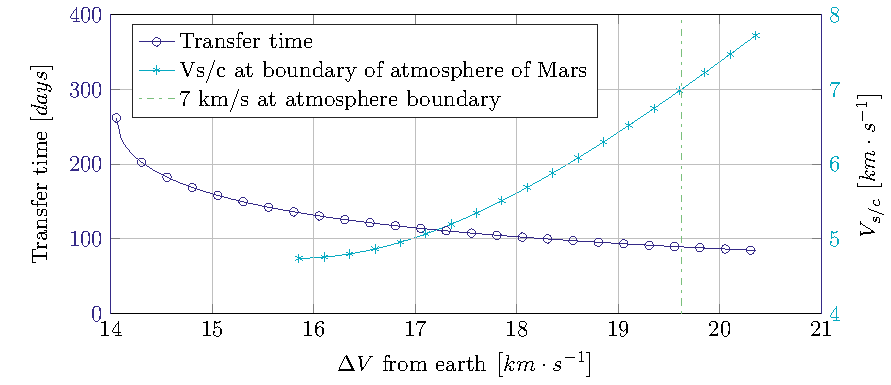
\includegraphics[width=0.95\textwidth]{Figure/Inter_transfer/transfer_time.pdf}
	\caption[Interplanetary transfer time and entry velocity versus $\Delta\gls{sym:V}$]{Interplanetary transfer time (left) and entry velocity (right) versus $\Delta\gls{sym:V}$}
	\label{fig:inter_time}
\end{figure}

The most efficient transfer with respect to the $\Delta\gls{sym:V}$-budget consists of a Hohmann transfer orbit. This would take approximately 262 days. This time is the longest of all orbits to Mars with a direct transfer. One of the mission requirements is the entry velocity of $7 \left[km \cdot s^{-1}\right]$. This velocity is fully determined by the $\Delta \gls{sym:V}$ budget and thereby corresponds to the transfer time. In Figure \ref{fig:inter_time} this relation is visualised. As can be seen to arrive with the required velocity a $\Delta \gls{sym:V}$ of $19.62 \left[km \cdot s^{-1}\right]$ is required, which corresponds to a transfer time of $89.3$ days. The corresponding orbit is shown in Figure \ref{fig:inter_orbit}.

\begin{figure}[h]
	\centering
	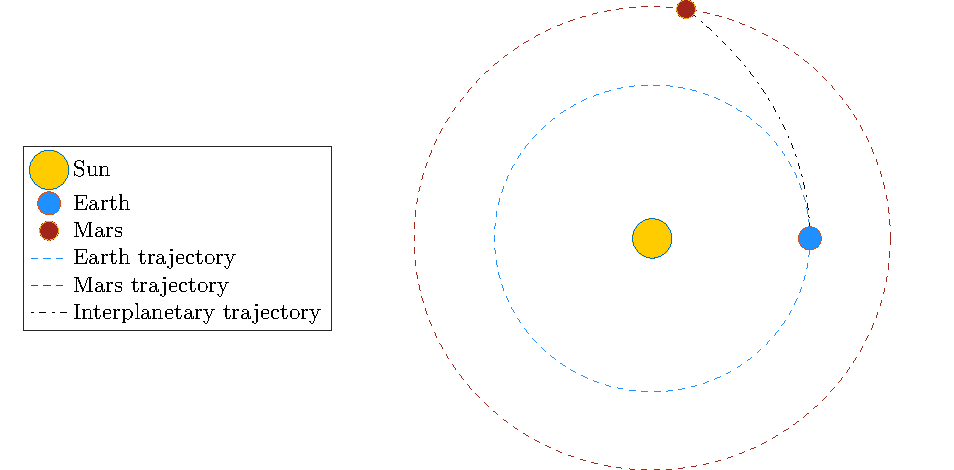
\includegraphics[width=0.95\textwidth]{Figure/Inter_transfer/orbits.pdf}
	\caption[Visualisation of the interplanetary transfer orbit]{Visualisation of the interplanetary transfer orbit. Planets not to scale}
	\label{fig:inter_orbit}
\end{figure}


\subsubsection{Aerocapture and entry} \label{sec:entry}
The third phase of the mission is the arrival at Mars and the deceleration to a velocity of $M=5$ at $15$ $\left[km\right]$ height above the surface of Mars with an accuracy of $500 \left[m\right]$ in each direction. This deceleration is split into an initial aerocapture, a parking orbit and a final entry. The combined sum of these components should not take longer than 10 Earth days. In this phase of the mission the \gls{hiad} is used to decelerate the capsule and protect it against the thermal loads imposed by the deceleration. In addition, taxation of human crew members requires loads not to exceed 3\gls{con:ge}.

%Upon arrival on Mars, first the interplanetary habitat is separated from the entry capsule. The habitat will be put on a trajectory which causes it to burn up in the vicinity of the sun.
Upon arrival at Mars the first thing that happens, just before the spacecraft enters the atmosphere, is the deployment and inflation of the \gls{hiad}. %The aeroshell will be continuously kept at pressure during the rest of the mission phase.
%The spacecraft is now transformed into a entry vehicle and is ready to start the aerocapture.

The entry vehicle then enters the atmosphere for the first time. This first pass through the atmosphere is called aerocapture. The entry vehicle will fly through the atmosphere following a pre-determined path using active bank control. A real-time controller will manage the active control systems to account for unexpected differences in atmospheric properties. The goal of this controller is to keep the kinetic energy lost during the aerocapture equal to what is pre-calculated. This loss of kinetic energy determines the characteristics of the trajectory which the spacecraft will follow once it leaves the atmosphere. %Diminishing too little energy causes the trajectory to be more eliptic or even hyperbolic. Diminishing too much energy causes the the trajectory to be less eliptic, or it can even cause the entry vehicle to not even go out of the atmosphere anymore. These trajectory characteristics change the orbit period and the fuel fraction needed to change 

After the aerocapture the spacecraft goes into an elliptic Kepler orbit. When the spacecraft is headed to the apocentre of the orbit it changes attitude so that the thrusters point in the along-path direction to give the spacecraft a velocity change. While in the apocentre the spacecraft gets a $\Delta\gls{sym:V}$ to raise the pericentre altitude of the Mars-centred orbit to a parking orbit at 200 $[km]$ height.
%In the apocentre the spacecraft gets a velocity change which will get it in an elliptic Mars-synchronous orbit which will not pass through the atmosphere. 

From this parking orbit the atmospheric conditions can be observed and a plan can be made for the entry into the atmosphere in order to get to the intended landing location. The observations made of the atmosphere will help determine a suitable moment to do the final entry and will give information that can be used to predict the final entry trajectory more accurately. For example, in case of a dust storm, characteristic of Mars, \gls{edl} can be delayed until it has passed.

Once the decision has been made to conduct the final entry the spacecraft is given a second boost to decelerate it just enough to get the entry vehicle into the desired trajectory. Here, just as during the first pass through the atmosphere, the spacecraft is controlled using active bank control managed by a real-time controller. %When the entry vehicle is approaching the intended final location at $10 \left[km\right]$ height a change in angle of attack is used to dive to that location. Having control over the time of initiation of the dive gives us an additional safety on landing within  $500 \left[m\right]$ from the target.

\subsubsection{Terminal descent} \label{sec:terminal}
The terminal descent of the spacecraft is the part of the mission between the end of aerocapture and landing on the surface of Mars. The velocity is to be brought back to zero at an altitude of zero, from an initial velocity at the end of the aerocapture phase of the mission. For the terminal descent, several design options are available to decrease the velocity. In this section, firstly, the mission characteristics are discussed. After that, the design options are summarized after which a choice is made based on feasibility and performance.

\paragraph{Terminal descent characteristics}
The start of this part of the mission is given by the end of the aerocapture part, of which the requirements dictate a Mach number of $5$ at a height of $15$ [km], as given in Section \ref{sec:missionreq}. This means the aerodynamic flow regime changes from hypersonic to supersonic, and finally to subsonic during the terminal descent. The speed of sound in the lowest fifteen kilometres of Mars is approximately $220$ $[m\cdot s^{-1}]$, which means the velocity of the spacecraft is $1100$ $[m\cdot s^{-1}]$ at the beginning of terminal descent. The velocity only marginally increases due to the gravity influence of Mars: the velocity with no deceleration would be 3 percent higher on the surface of Mars than at an altitude of $10$ $[km]$, assuming no deceleration due to drag or thrust. Finally, the flight path angle is not predetermined by the orbit, so it can be changed to fit the needs of the terminal descent phase.

\paragraph{Design options}
Terminal descent can be split up in two parts: the supersonic and subsonic flight part and final touchdown. For both parts, different options are available.

The first option for the flight is to use retro-propulsion for every part of the descent. The fuel mass would be about $23.3\%$ of the total spacecraft mass if no aerodynamic effects were taken into account. However, the aeroshell has a large frontal area which adds a significant amount of drag. Also, in numerical simulations and wind tunnel tests the interaction between retro-propulsion and the aeroshell were found to result in a mass fraction that is approximately twice as small as would be expected when considering the thrust and drag forces to act independently of each other \cite{Korzun2009}. Since a blunt body is unstable at transonic and supersonic speeds, a small drogue parachute is needed to stabilise the spacecraft. Scaling a mass estimate for an inflatable aeroshell from NASA, this stabilisation drogue parachute is approximately 20 [kg] including 20$\%$ contingency.
The fuel mass is estimated assuming a constant deceleration of 3 [\gls{sym:ge}]. This condition in combination with the initial conditions of the terminal descent, leads to a specified flight path angle of 38 [deg] and a velocity at each height. Using this velocity, the drag was calculated assuming the same drag coefficient throughout the supersonic regime. This analysis is known to be incorrect to a certain level, but since it is preliminary analysis this is taken for granted. The drag at every height leads to a deceleration lower than 3 [\gls{sym:ge}], and thrust is delivered at a level such that this deceleration is achieved, incorporating the gravitational force. The drag, thrust and total required force are plotted in Figure \ref{fig:TDforce}. This requires the rocket engines to be sized such that, a total thrust of 312 [kN] is achieved. To this end, 3 RL 10A-4 rocket engines are placed at the front of the centerbody. The mass of these rockets is 504 [kg] combined. The thruster fuel flow is calculated using the specific impulse of the engine, 451 [s], and integrated over time to find the total fuel, estimated to be 680 [kg] \cite{Wertz2011}. The tank mass is estimated using an empirical relation, at 45 [kg] and assuming a density of 1 $[kg\cdot dm^{-3}]$ for the fuel \cite{Wertz2011}.

\begin{figure}
	\centering
	\setlength\figureheight{0.4\textwidth} 
	\setlength\figurewidth{0.7\textwidth}
	\input{./Figure/TerminalDescent/TDthrust.tikz}
	\caption{Thrust, drag and required force for 3 [\gls{sym:ge}] deceleration starting from 15 [km] height at $M=5$}
	\label{fig:TDforce}
\end{figure}


The other option is to use a large parachute to decelerate. Since a parachute's performance decreases quadratically with lower velocities, the final landing still requires thrusters to bring the velocity down to an acceptable value for landing \cite{Braun2007}. The difference in fuel mass was estimated by using a parachute with a diameter of 30 [m] and a drag coefficient of 0.3, deployed at the moment in time where the added drag of the parachute would make the total acceleration 3 [\gls{sym:ge}]. For these conventional figures, the fuel mass loss was approximately 200 [kg], while the added mass of a parachute is approximately 280 [kg] per an empiric relation \cite{Anderson1969}. This is added to the fact that the atmospheric density on Mars offers unacceptable parachute deployment \cite{Korzun2009}.

The final touchdown can happen by carefully manoeuvring the spacecraft with thrusters to land on legs. These were estimated to have a mass of 200 [kg], as estimated using a structural sizing for a smaller spacecraft to be landing on Mars.\footnote{\url{http://www.nasa.gov/pdf/458812main_FTD_AerocaptureEntryDescentAndLanding.pdf}. Accessed: 18-06-2015} The other option is to land using airbags, as was performed by for example the Mars Pathfinder. However, this induces high peak accelerations during the landing and introduces uncertainties in landing location since the airbag bounces before coming to a stop.

\paragraph{Terminal descent design}
The final design of the terminal descent stage of the mission is chosen te be a retro-propulsion deceleration, using 3 rocket engines that total 504 [kg], with a 680 [kg] fuel usage throughout terminal descent, and a fuel tank of 45 [kg]. The landing gear has an estimated mass of 200 [kg] and will be deployed while still in the air. After that, the inflatable structure is deflated to make it lose it's stiffness and allow the landing gear to touch the ground, as explained in Section \ref{subsec:crewtermdescent}. The stabilisation drogue parachute has a mass of 20 [kg]. Adding up the component masses gives the total terminal descent mass of 

%\subsubsection{Ground operations} \label{sec:groundop}
%It is important that the ground segment is taken into a consideration at this stage to assess mission feasibility and to provide an early impression of the required ground facilities. The ground segment is an essential mission feature to facilitate communication flow between Earth and spacecraft and thereby to monitor mission progress and crew member status as well as take corrective actions if need be and circumstances allow.

To this end, the ground segment consists of a missions operations centre and a communications network. This set-up is similar to \gls{esa} ground operations for deep space missions Rosetta and Venus Express\footnote{URL: \url{http://www.esa.int/esapub/bulletin/bulletin124/bul124e_warhout.pdf}. Accessed: 10-06-2015}  \cite{Warhaut2007}. An alternative would be a decentralized structure, in which control centres are not included in the missions operations centre but linked separately to it. 

\paragraph{Operations centre}
The operations centre is manned continually with the purpose of monitoring and controlling mission progress \cite{Warhaut2007}. It is the ground system element that is in direct contact with the spacecraft by the link established through the ground stations for uplink and downlink \cite[p.879]{Wertz2011}. Downlink data are analysed and formatted, partially sent through to the end-receivers of scientific information and partially used for mission health monitoring and control. The nature of these end-receivers of scientific information depends on the payload activities conducted on Mars. 

Examples of such an operations centre are the California Institute of Technology's Jet Propulsion Laboratory, responsible for NASA's \gls{dsn}, or the \gls{esoc}, responsible for \gls{esa} deep space missions. The former has been used for one for the manned Apollo missions to the moon, the latter for Rosetta and Apollo missions \cite{Wertz2011,Warhaut2007}. Both of these operations centres would be suitable for the mission at hand, mainly due to their successful operation in past deep space and manned missions. 

\paragraph{Communications network}
A communication link is established between the ground segment and the spacecraft. Key feature is its ability for communication between Mars and Earth, over which free space losses are highly significant \cite{Wertz2011}. While manned missions to Mars have not been flown, a good reference point is a previous unmanned Mars mission, such as the Mars Rover, as both face similar communication requirements. The Mars Rover was reliant on the \gls{dsn}\footnote{URL: \url{http://mars.nasa.gov/mer/mission/communications.html}. Accessed: 10-06-2015} for its communications on X-band. 

The \gls{dsn} uses three complexes separated by 120 degrees of longitude to provide continual coverage with a rotating Earth. Sensitive 70 [$m$] diameter antennas are used for maximum sensitivity and complemented by a number of 34 [$m$] diameter antennas. \cite{Wertz2011} These antennas would be suitable for the mission at hand by their intended and proven purpose of providing communication in deep space and therefore to and from Mars. While the technology is thereby sufficient, continuous maintenance of and improvements on the \gls{dsn} will ensure proper functioning and network availability over the next decades. An alternative would be \gls{esa}'s ESTRACK, consisting of $10$ \gls{esa} operated ground stations for communication support. These do not allow for Ka-band transmission, however \cite{Wertz2011}.

Bandwidths are required to allow for sufficient signal strength upon reception and additionally follow from the required bit rate. Current standard for deep space missions are S-band, in a frequency range of 2.0-2.3 [$GHz$], and X-band, in a frequency range of $8.45$ to $8.50$ [$GHz$] \cite{Wertz2011}.

An advancing trend is the use of Ka-band for deep space communication downlink, in a frequency range of $25.5$-$32.3$ [$GHz$]. Ka-band is able to provide more data volume in less \gls{dsn} tracking time, while continuing automation for \gls{dsn} ground systems will further increase antenna availability through a reduction of required calibration time\cite{Edwards1999}. 

Following requirements on NASA's \gls{dsn} S-band will be available for both up- and downlink, while Ka-band will be available for high-data-rate science returns \cite{Labelle2012}. The crew module itself will not necessitate Ka-band for the purpose of science returns, but transmission of detailed system state measured by sensors for the purpose of monitoring will benefit from the use of a Ka-band for downlink. For the purpose of uplink, limited communication flow is present and S-band suffices.%Uplink will merely require communication with on-board payload, since the spacecraft is predominantyl autonomous by the excessive transfer time of ground-based commands and thereby inability to otherwise react

As such, Ka-band is used for downlink telecommunication for its high data link capability, while S-band is used for uplink. Both are supported by the \gls{dsn}.


\subsubsection{Return} \label{sec:return}












\subsection{Ground segment} \label{sec:gop}
It is important that the ground segment is taken into consideration at this stage to assess mission feasibility and to provide an early impression of the required ground facilities. The ground segment is an essential mission feature to facilitate communication flow between Earth and spacecraft and thereby to monitor mission progress and crew member status as well as take corrective actions if needed and circumstances allow.

To this end the ground segment consists of a missions operations centre and a communications network. This set-up is similar to \gls{esa} ground operations for deep space missions Rosetta and Venus Express\footnote{URL: \url{http://www.esa.int/esapub/bulletin/bulletin124/bul124e_warhout.pdf}. Accessed: 10-06-2015}  \cite{Warhaut2007}. An alternative would be a decentralised structure, in which control centres are not included in the missions operations centre but linked separately to it. 

\paragraph{Operations centre}
The operations centre is manned continually with the purpose of monitoring and controlling mission progress \cite{Warhaut2007}. It is the ground system element that is in direct contact with the spacecraft via the link established through the ground stations for uplink and downlink \cite[p.879]{Wertz2011}. Downlink data is analysed and formatted, partially sent through to the end-receivers of scientific information and partially used for mission health monitoring and control. The nature of these end-receivers of scientific information depends on the payload activities conducted in-flight and on Mars. 

Examples of such an operations centre are the California Institute of Technology's Jet Propulsion Laboratory, responsible for NASA's \gls{dsn}, or the \gls{esoc}, responsible for \gls{esa} deep space missions. The former has been used for one for the manned Apollo missions to the moon, the latter for Rosetta and Apollo missions \cite[p.883]{Wertz2011}\cite{Warhaut2007}. Both of these operations centres would be suitable for the mission at hand, mainly due to their successful operation in past deep space and manned missions. 

\paragraph{Communications network}
Key feature of the communications network ability for communication between Mars and Earth, over which free space losses are highly significant \cite{Wertz2011}. While manned missions to Mars have not been flown, a good reference point is a previous unmanned Mars mission, such as the Mars Rover, as both face similar communication requirements. The Mars Rover was reliant on the \gls{dsn}\footnote{URL: \url{http://mars.nasa.gov/mer/mission/communications.html}. Accessed: 10-06-2015} for its communications on X-band. 

The \gls{dsn} uses three complexes separated by 120 degrees of longitude to provide continual coverage with a rotating Earth. Sensitive 70 $[m]$ diameter antennas are used for maximum sensitivity and complemented by a number of 34 $[m]$ diameter antennas \cite{Wertz2011}. These antennas would be suitable for the mission at hand by their intended and proven purpose of providing communication in deep space and to and from Mars. While the technology is thereby sufficient, continuous maintenance of and improvements to the \gls{dsn} will ensure proper functioning and network availability over the next decades. An alternative would be \gls{esa}'s ESTRACK, consisting of $10$ \gls{esa}-operated ground stations for communication support. However, these do not allow for Ka-band transmission \cite[p.631]{Wertz2011}.

Bandwidths are required to allow for sufficient signal strength upon reception and additionally follow from the required bit rate. The current standards for deep space missions are S-band, in a frequency range of $2.0$-$2.3$ $[GHz]$, and X-band, in a frequency range of $8.45$-$8.50$ $[GHz]$ \cite{Wertz2011}.

An advancing trend is the use of Ka-band for deep space communication downlink, in a frequency range of $25.5$-$32.3$ [$GHz$]. Ka-band is able to provide more data volume in less \gls{dsn} tracking time, while continuing automation for \gls{dsn} ground systems will further increase antenna availability through a reduction of required calibration time \cite{Edwards1999}. 

Following requirements on NASA's \gls{dsn} S-band will be available for both up- and downlink, while Ka-band will be available for high-data-rate science returns \cite{Labelle2012}. The crew module itself will not necessitate Ka-band for the purpose of science returns, but transmission of detailed system state measured by sensors for the purpose of monitoring will benefit from the use of a Ka-band for downlink by a high required data rate. For the purpose of uplink, limited data flow is present and S-band suffices.%Uplink will merely require communication with on-board payload, since the spacecraft is predominantly autonomous by the excessive transfer time of ground-based commands and thereby inability to otherwise react

As such, Ka-band is used for downlink telecommunication for its high data link capability, while S-band is used for uplink. Both are supported by the \gls{dsn}. 

Due to the long transfer time between the spacecraft and Earth, it is key that the delay in communication is taken into account and the spacecraft is self-reliant rather than dependent on ground instructions. As such, the on-board computer is autonomous with a manual override for crew members.

\subsection{Mission scope} \label{sec:missionscope}
Whereas Section \ref{sec:missionoutline} covers the entire mission from launch to return on Earth the focus of this report lies with the aerocapture into a parking orbit around Mars, together with the subsequent aerobraking. To achieve this a \gls{hiad} has been designed, based on the requirements covered in Section \ref{sec:missionreq}. Even though the mission of the \gls{hiad} is concerned with the entry procedure described in Section \ref{sec:entry} the other mission elements also carry an effect on its design. From the launch mentioned in Section \ref{sec:launch} follows that the \gls{hiad} must be able to withstand the launch loads and vibrations. 

Following launch, Earth orbit and subsequent acceleration into a heliocentric orbit the interplanetary flight segment of the mission takes place, as described in section \ref{sec:interplanetary}. From this mission segment comes the requirement for the deceleration capability of the \gls{hiad}, a shorter interplanetary transfer time results in a higher velocity with respect to Mars. This is further covered in section \ref{sec:missionreq}. 

When the capsule carrying the crew arrives at Mars with its accompanying modules and systems required for interplanetary transfer the actual mission of the \gls{hiad} takes place. It is this mission segment that forms the scope of this report and is where the \gls{hiad} performs its function. The aerocapture, travel while in a parking orbit and subsequent initiation of the terminal descent procedure can take up to ten days altogether. After the terminal descent \& entry procedure has been initiated the aeroshell will be retained to aid in the final descent and deceleration until touchdown.

As such, the considerations in this chapter on the entire mission and the crew capsule design in Chapter \ref{ch:crewmod} are conceptual suggestions for further design efforts. To this end, their main purpose is to investigate the compatibility of the \gls{hiad}, crew module and mission. Other design options for the crew module remain possible.

\subsection{Mission requirements} \label{sec:missionreq}
In this section the mission requirements for the mission as described in Section \ref{sec:missionscope} are outlined and their origin is explained. A full list of requirements as defined top level can be found in Table \ref{tab:misreq} and \ref{tab:vehreq}.

The mission starts at the boundary of the atmosphere of Mars. Here the velocity of the entry vehicle is $7 \left[km \cdot s^{-1} \right]$. This requirement is imposed by the transfer trajectory that is taken from Earth to Mars. This trajectory should take as short as possible in order to both shorten the entire mission duration and decrease the physical taxation on the crew. The interplanetary transfer time corresponding to an entry velocity of $7 \left[km \cdot s^{-1} \right]$ is $89$ days. 

The mission ends at a speed of $M=5$ at $15 \left[km\right]$ altitude. At this point a terminal descent system takes over. The predetermined point at which the mission ends shall be reached with a precision of $500 \left[m\right]$. This requirement is imposed by the distance the final landing position can be from the provision. When the landing position lies too far from the provision a lot of time will be lost relocating the crew or crew members might not even be able to reach the provision.

While decelerating in the atmosphere the maximum deceleration shall not exceed 3\gls{con:ge}. This requirement is imposed because of the limited capability of the crew to carry high deceleration loads.

The entry vehicle should attain its final velocity within 10 earth days. This requirement is, just like the interplanetary transfer time, imposed both to shorten the mission duration and decrease the physical taxation on the crew. An additional reason for this time constraint is to limit the cost for and strain on the ground control crews that will be active continuously during the mission.


\begin{table}[h]
	\caption{Overview of mission requirements}
	\label{tab:misreq} 
	\begin{tabular}{|p{0.12\textwidth}|p{0.85\textwidth}|}
    \hline
    \textbf{ID}          & \textbf{Description}                                                                                                      \\ \hline \hline
    CIA-M01& The entry vehicle shall decelerate from a velocity of 7 $[km\cdot s ^{-1}]$ at 400 [$km$]  \\ \hline
    CIA-M02 & The entry vehicle shall not exert an acceleration greater than 29.4 $[m \cdot s^{2}]$ on any crew member for the duration of the mission			\\ \hline
    	CIA-M03 & The entry vehicle shall attain reach Mach 5 $[-]$ at an altitude of 15 000 $[m]$  \gls{mola} \\ \hline
    	CIA-M04 & The entry vehicle shall reach its final position with a precision of 500 $[m]$\\ \hline
    	CIA-M05 & The entry vehicle shall attain its final velocity within 10 days of mission start \\ \hline
    \end{tabular}
\end{table}

\begin{table}[h]
	\caption{Overview of entry vehicle requirements} 
	\label{tab:vehreq}
	\begin{tabular}{|p{0.12\textwidth}|p{0.85\textwidth}|}
	    \hline
	    \textbf{ID}          & \textbf{Description}                                                                                                     \\ \hline \hline
	CIA-R01 & The entry vehicle shall have an undeployed diameter smaller than 5 $[m]$                         				            \\ \hline
	CIA-R02 & The entry vehicle shall have a deployed diameter smaller than 12 $[m]$                         				            \\ \hline	
	CIA-R03 & The entry vehicle shall have a mass of 10 000 $[kg]$ at the start of the entry                       				            \\ \hline
	CIA-R04 & The hypersonic decelerator shall have a mass fraction of no greater than $10\%$ of the vehicle mass  \\ \hline
	CIA-R05 &  The entry vehicle shall adhere to the \gls{cospar} regulations \\ \hline
	CIA-R06 &  The entry vehicle shall have control system accuracy of at least $5\cdot 10^{-4}$  \\ \hline
    \end{tabular}
\end{table}

\subsection{Market analysis} \label{sec:marketanalysis}
\section{Market analysis} \label{ch:market}

\subsection{Sustainable development strategy} \label{sec:sustainable}
Increasing awareness with respect to sustainable development makes sustainability a important considerations within the design. Masud et al. define development as being sustainable "by ensuring the needs of the present demands without compromising any power or ability of future generations to meet their own needs" \cite[p.85]{Masud2011}. 

Within the scope of the mission sustainability is considered where possible. It must however be considered that the production series length is small and less emphasis is given to sustainable development when compared to (for example) a commercial passenger jet. As such the aeroshell's overall environmental impact is negligible and the sustainability of the concepts discussed in this report is not taken into account as a strong design driver. Never the less important consideration may be taken. 

Decelerator structural mass reductions directly allow for increases in useful payload, or allow for the use of smaller launchers for the same mission. By doing so the footprint of each launch may be reduced for comparable missions. For the \gls{mtr}, summarized in Chapter \ref{cha:conceptselection},  a conventional rigid solution was investigated. Preliminary mass estimates were over a factor three larger than the design presented within this final report. Choosing such a conventional concept would not only violate the mission requirements but would also incur additional emission during the initial launch.

Sustainability is also taken into account outside of the Earth's atmosphere. Special care will be given to prevent accidental contamination of other orbital bodies with organic lifeforms and other contaminants. This is in line with article IX of the Outer Space Treaty of 1967 \cite{UnitedNations2008}, enforced by the \acrfull{cospar}. Moreover the materials used in space are considered where possible. One such example is the use of nitrogen as the final inflation gas as further detailed in Chapter \ref{subsec:inflsys}. Less sustainable inflation gasses could be considered, such as for example hydrazine, which could achieve marginal mass reductions. From a sustainability point of view such a option was not preferred.




 ...WORK IN PROGRESS...



%\section{Approach with respect to sustainable development}
%\label{ch:sustain}
%
%With a increasing awareness with respect to sustainable development it is important to consider mission sustainability. This chapter discusses the approach with respect to sustainable development of the \gls{hiad} design concepts at hand. Masud et al. define development as being sustainable "by ensuring the needs of the present demands without compromising any power or ability of future generations to meet their own needs" \cite[p.85]{Masud2011}.
%
%Since the production series length of the controllable inflatable aeroshell is limited to very low numbers less emphasis is given to sustainable development when compared to (for example) a commercial passenger jet. As such the aeroshell's overall environmental impact is negligible and the sustainability of the concepts discussed in this report is not taken into account as a strong design driver. That is not to say sustainability is completely disregarded during product development. If for a certain design manufacturing methods are required that are very polluting these will be avoided and exchanged for less environmentally unfriendly, 'greener' methods. 
%Not only sustainability on Earth is taken into account, but also the impact of a space mission to another orbital body on the environment of said body is considered. Special care will be given to prevent accidental contamination of other orbital bodies with organic lifeforms and other contaminants. This is in line with article IX of the Outer Space Treaty of 1967 \cite{UnitedNations2008}, enforced by the Committee on Space Research (COSPAR). In addition to preventing forward interplanetary contamination care will be taken to minimise the amount of space debris left behind in an orbit around Earth and Mars. 
%
%The development of a controllable inflatable aeroshell can however improve the sustainability of both planetary and interplanetary spaceflight. Since implementing an inflatable aeroshell contributes to reducing the total mass of a spacecraft this can reduce the required launcher mass and thereby the launch emissions. The differences with respect to sustainability between the different concepts to be analysed is very small and is thus not used as a separate element in the trade-off process.
%
%Going back to the definition of sustainable development presented at the beginning of this chapter one can see that the measures taken during the design are indeed in line with sustainable development.
%




\subsection{Cost breakdown structure} \label{sec:costbreakdown}
Cost can be split up into two sections: Development cost and production cost. Whereas the development-related costs consist of non-recurring expenses, the production cost is dependent on the number of missions to be carried out. The analysis by Wertz et al. \cite{Wertz2011} will be used to determine the costs associated with these components. Since these are determined in constant 2010 US dollars a factor accounting for inflation is used. This factor was found by looking at the \gls{cpi} ratio between April of 2010 and 2015. From Reference \cite{Crawford2015} this factor was found to be $1.075$, corresponding to an inflation over five years of $7.5\%$.\\
For the development and production cost a \gls{hiad} propellant mass of $153$ $\left[kg\right]$ was used, conform to the final design presented in Chapter \ref{cha:finaldesign}. A total \gls{hiad} mass (including propellant) of $1000$ $\left[kg\right]$ was assumed, in order to take into account the maximum allowable \gls{hiad} mass growth. For the crew capsule a total mass of $9000$ $\left[kg\right]$ was assumed from which $700$ $\left[kg\right]$ of propellant mass was subtracted. The origin of this propellant mass will be covered in further detail in Chapter \ref{ch:crewmod}. In addition to the propellant mass the crew mass was also subtracted in order to arrive at the spacecraft dry mass.\\
Next to the \gls{hiad} and accompanying crew module a \gls{mav} and an \gls{erv} are also needed to complete the mission. These vehicles fall outside of the scope of this report, but in order to estimate their impact on mission cost they will be taken into account in this section. A dry mass of $5000$ and $10$ $000$ $\left[kg\right]$ was assumed for these vehicles respectively.

\subsubsection{Development costs}
In contrast to the total mission the development costs consist of those incurred by aeroshell and capsule development. Atgar \cite[p.296]{Wertz2011} presents the development cost per kilogram of dry mass for various vehicles. These values, together with the total development cost are shown in Table \ref{tab:devcosts}.

\begin{table}
	\centering
	\caption{Development costs in 2015 US dollars}
	\begin{tabular}{|c|p{5cm}|p{5cm}|}
		\hline
		\textbf{Cost component} & \textbf{Development cost per kg dry mass $\mathbf{[2015}$ $\mathbf{US\$]}$} & \textbf{Total development cost $\mathbf{[2015}$ $\mathbf{million \mbox{ } US\$]}$} \\ \hline \hline
		Aeroshell & 2 569 000 & 2 176 \\
		Crew module & 1 255 000 & 10 216 \\
		\acrlong{mav} & 2 569 000 & 12 845  \\
		\acrlong{erv} & 1 255 000 & 12 550  \\ \hline
		\textbf{Total} & - & 37 786 854 \\
		\hline
	\end{tabular}
	\label{tab:devcosts}
\vspace{-2mm}
\end{table}

\subsubsection{Production costs}
The production costs were determined in similar fashion to the development costs presented in the previous section. Table \ref{tab:productioncosts} shows the corresponding productions costs per kilogram of dry spacecraft mass and for the complete respective component.

\begin{table}[h]
	\centering
	\caption{Production costs in 2015 US dollars}
	\begin{tabular}{|c|p{5cm}|p{5cm}|}
		\hline
		\textbf{Cost component} & \textbf{Production cost per kg dry mass $\mathbf{[2015}$ $\mathbf{US\$]}$} & \textbf{Total production cost $\mathbf{[2015}$ $\mathbf{million \mbox{ } US\$]}$} \\
		\hline \hline
		Aeroshell & 341 000 & 289 \\
		Crew module & 173 000 & 1 408 \\ 
		\acrlong{mav} & 341 000 & 1 705 \\
		\acrlong{erv} & 173 000 & 1 730 \\ \hline
		\textbf{Total} & - & 5 132 \\
		\hline
	\end{tabular}
	\label{tab:productioncosts}
\vspace{-2mm}
\end{table}

\subsubsection{Mission costs}
In addition to the costs incurred by the spacecraft themselves the overall mission architecture requires the use of additional resources such as launch vehicles. Assuming that two \glspl{sls} are needed to position all required vehicles mentioned in Section \ref{sec:missionoutline} around Mars (including the mission carrying the \gls{hiad} and associated crew module) the mission item cost can be determined by summing these launch costs with the aforementioned production costs. For the launch of the \gls{sls} no official cost figure exists, though \gls{nasa} officials have been quoted as mentioning a goal of $500$ million US dollars per launch\footnote{URL: \url{http://www.nbcnews.com/id/49019843/ns/technology_and_science-space} Accessed: 18-06-2015}. As such the total launch cost adds up to 1 billion US dollars.

%A more realistic 1 billion US dollars estimate is favoured to this optimistic estimate.

\begin{table}[H]
	\centering
	\caption{Overview of total costs for one mission}
	\begin{tabular}{|c|c|}
		\hline
		\textbf{Cost component} & \textbf{Cost $\mathbf{[2015}$ $\mathbf{million \mbox{ } US\$]}$} \\ \hline 
		\hline
		Vehicle development & 37 787 \\
		Vehicle production & 5 132\\
		Launch & 1 000\\ \hline
		\textbf{Total} & 43 919\\ \hline
	\end{tabular}
	\label{tab:missioncosts}
\end{table}

By combining the cost figures presented here the results presented in Table \ref{tab:missioncosts} were obtained. If more than one mission using these spacecraft is to be conducted the average cost per mission will be considerably lower than the total cost presented in Table \ref{tab:missioncosts} since the development costs are non-recurring expenses. This would also increase the cost-effectiveness of manned spaceflight to Mars.

%\subsection{Operation and logistics} \label{sec:operations}
%






\section{Concept selection}\label{cha:conceptselection}
This chapter describes the steps leading up to the selection of the stacked toroid concept. This concept has been found to yield the most favourable combination of characteristics and was therefore selected for further analysis. Concepts have been generated in a structured way using a design option tree, as described in Section \ref{sec:conceptgen}. Subsequently, concepts were evaluated for four trade-off criteria, defined in Section \ref{sec:conceptcriteria}. This yields an overview of relative concept performance, summarised in Section \ref{sec:conceptperf}.


A more detailed overview of the trade-off process is given in the Mid-Term Report \cite{Balasooriyan2015b}.

\subsection{Concept generation} \label{sec:conceptgen}
Concepts were generated on the basis of decelerator configuration, the leading design parameter to distinguish concepts. On the basis of the shape \gls{dot} given in Figure \ref{fig:dotshape}, five blunt bodies were selected for the trade-off process. Four inflatable concepts were selected alongside one rigid concept to fully appreciate the advantages inflatable concepts offer.

\begin{figure}[h]
%\centering
\hspace{-23mm}
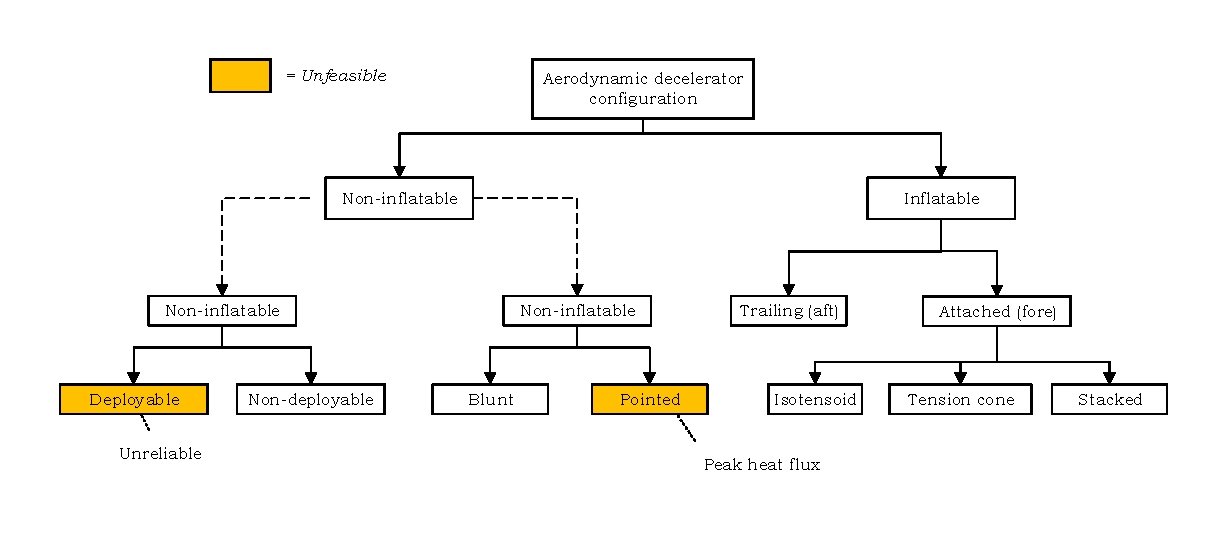
\includegraphics[width = 1.25\textwidth]{Figure/Concepts/DOT_configuration.pdf}
\vspace{-5mm}
\caption{\acrlong{dot} for entry vehicle configuration}
\label{fig:dotshape}
\end{figure}

Non-inflatable deployable concepts offer a lower reliability than and no particular advantages with respect to inflatable concepts and were therefore discarded. Pointed shapes were found infeasible by the peak heat flux generated. Lastly, combined inflatables were discarded since these add system complexity and mass while offering no additional advantages. 

Artist impressions of the resulting five concepts are given in Figure \ref{fig:concepts}. The concepts are:
\begin{itemize}
\item[(a)] A rigid concept, the conventional solution for re-entry. Its absence of deployment and its thereby limited diameter necessitates the use of a backshell to prevent the side of the payload capsule from excessive heating \cite{Hughes2005}.
\item[(b)] An isotensoid, a flexible bladder encapsulating the crew module that is inflated by ram-air through inlets mounted on it.
\item[(c)] A stacked toroid concept, in which multiple flexible rings are stacked on top of one another and inflated by an internal inflation system.
\item[(d)] A tension cone concept, which features one internally inflated torus and a flexible membrane that is spanned between the torus and the rigid centre body.
\item[(e)] A trailing ballute concept, the sole concept with a trailing inflatable. The inflated torus is connected to the payload capsule by a multitude of cables.
\end{itemize}

\begin{figure}[h]
	\centering
	\begin{subfigure}[b]{0.32\textwidth}
		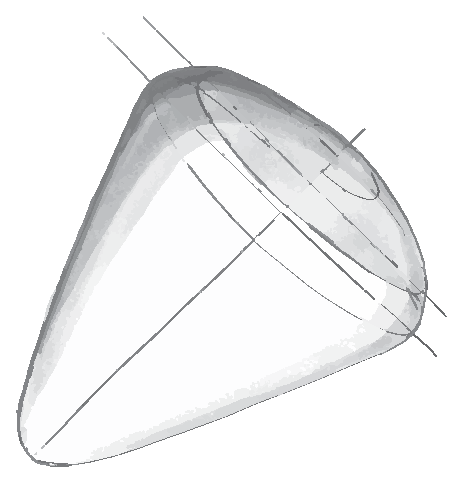
\includegraphics[angle=180, width=0.96\textwidth]{./Figure/Concepts/rigid.eps}
		\caption{Rigid concept}
		\label{fig:rigid}
	\end{subfigure}
	\begin{subfigure}[b]{0.32\textwidth}
		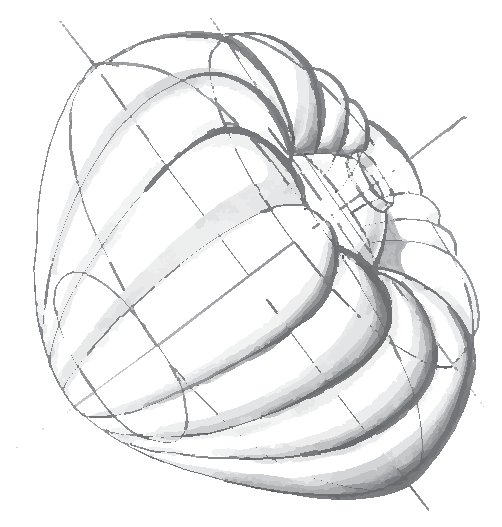
\includegraphics[width=0.96\textwidth]{./Figure/Concepts/isotensoid.eps}
		\caption{Isotensoid concept}
		\label{fig:isotensoid}
	\end{subfigure}
	\begin{subfigure}[b]{0.32\textwidth}
		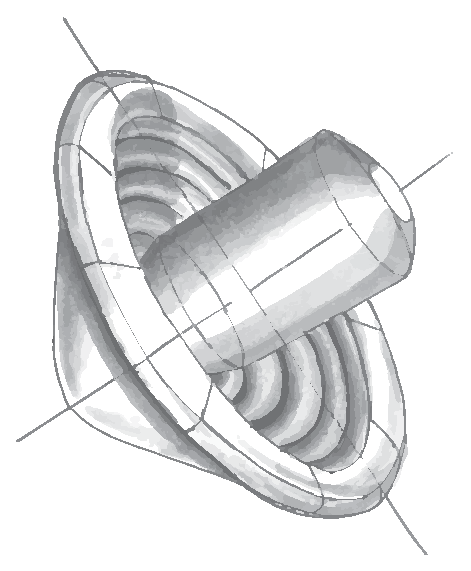
\includegraphics[width=0.96\textwidth]{./Figure/Concepts/stacked_toroid.eps}
		\caption{Stacked toroid concept}
		\label{fig:stacked_toroid}
	\end{subfigure}
	\begin{subfigure}[b]{0.32\textwidth}
		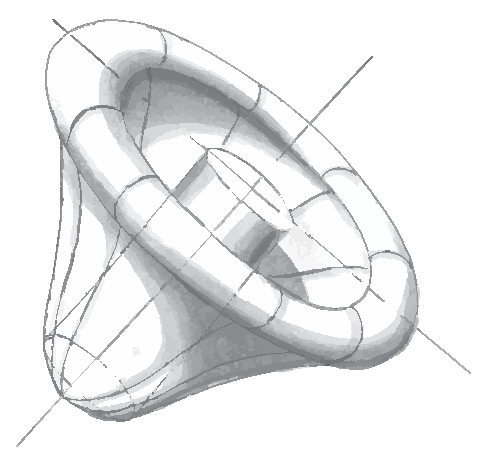
\includegraphics[width=0.96\textwidth]{./Figure/Concepts/tension_cone.eps}
		\caption{Tension cone concept}
		\label{fig:tension_cone}
	\end{subfigure}
	\begin{subfigure}[b]{0.32\textwidth}
		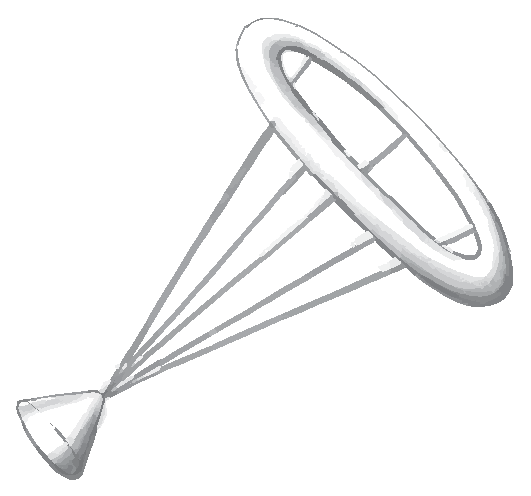
\includegraphics[width=0.96\textwidth]{./Figure/Concepts/trailing_ballute.eps}
		\caption{Trailing ballute concept}
		\label{fig:trailing_ballute}
	\end{subfigure}
\caption[Overview of design concepts]{Overview of design concepts (Courtesy of Irene Heemskerk)}
\label{fig:concepts}
\end{figure}






\subsection{Concept trade-off criteria} \label{sec:conceptcriteria}
Concepts have been evaluated on the basis of the following four criteria: decelerator mass, deceleration time, stability and development risk. These are discussed hereafter.

\subsubsection{Decelerator mass}
To take full advantage of launcher capability, the total vehicle mass is kept at its maximum. An increase in decelerator mass then leads to a decrease in payload mass, so it is essential that decelerator mass is kept to a minimum. To this end, the three primary components making up decelerator mass were evaluated for each concept: \gls{tps} mass, structural mass and control system mass. Their weighted average was computed to yield a total mass, taking into account their respective significance. The weight factors were determined from a comparable inflatable entry vehicle, namely \gls{irve} \cite{Hughes2005}.

The relative structural mass was determined using the structural mass estimation tool described in Section \ref{subsec:structool} and in more detail in the Mid-Term Report \cite[p.47-66]{Balasooriyan2015b}. Relative \gls{tps} mass is reflected by the estimated peak heat flux, a first-order estimation of the thermal energy to be dissipated and a key design driver for the \gls{tps}. Relative control system mass is reflected by the control moment required to be effected by the control system, in the form of the moment coefficient following from the aerodynamic analysis using modified Newtonian flow theory, as described in Section \ref{subsec:aerotool}. This was characterised by the lift-to-drag ratio, to account for the difference in lifting capability between concepts. Lower peak heat flux and low moment coefficients are favourable in terms of mass. 

\subsubsection{Deceleration time}
Minimising deceleration time is favourable for minimising ground operations expenses, since ground control is required to be fully active at the time of entry, which is the most critical mission phase. Furthermore, taxation of crew members is then alleviated. The time spent in the atmosphere is reflected by vehicle lift-to-drag ratio. For a given \gls{sym:CD}\gls{sym:A}, the maximum deceleration can be chosen by varying the lowest part of the trajectory: the density in lower parts of the atmosphere is higher, which then compensates for a low drag coefficient to produce the same force as a spacecraft with a high drag coefficient at a higher altitude with lower density. Because of the large variation of density in the atmosphere, it is possible to find a trajectory for any \gls{sym:CD}\gls{sym:A}. Thus, the drag coefficient itself is not a key driver for the design. However, the spacecraft can influence its deceleration time in the atmosphere by producing lift: if the spacecraft were to fly out of the atmosphere, a downward pointing lift would divert its trajectory more through the atmosphere. The ability of the spacecraft to influence this trajectory through the atmosphere is characterised by the amount of lift that can be produced, with respect to the amount of drag produced at the same \gls{sym:alpha}. The dependence on drag is due to the fact that two spacecraft with the same lift-to-drag ratio but a different \gls{sym:CD}\gls{sym:A}, will just have the lowest part of the trajectory at a different altitude, where the total lift and drag force will be the same for both spacecraft. Therefore, the deceleration time is characterised by the  lift-to-drag ratio. 

Lift and drag coefficients follow from the aerodynamic analysis tool, described in detail in the Mid-Term Report \cite[p.34-46]{Balasooriyan2015b}.

\subsubsection{Stability}
Vehicle stability is preferable, since a stable vehicle will react to disturbances with a restoring moment to revert to its original equilibrium condition without requiring control system activity. Not only does this reduce required control system activity, thereby limiting the system mass, but in addition the vehicle is more robust and less susceptible to perturbations. Stability is reflected by the static stability coefficient of concepts, following from aerodynamic analysis.

\subsubsection{Development risk}
It is key that concepts are evaluated for their development risk, an indication of schedule and cost risk. A concept with a high development risk will require extensive investigation to fully explore its capabilities and mitigate risks by technical uncertainty associated with such an underdeveloped concept. These investigation efforts incur additional cost and schedule risk. Development risk of concepts is evaluated by their \gls{trl}, denoting the current state of testing and application.





\subsection{Concept performance} \label{sec:conceptperf}
In terms of decelerator mass, the isotensoid was estimated to be the lightest concept, followed by the stacked toroid, illustrated in Table \ref{tab:cmass}. The tension cone and trailing ballute were notably heavier, primarily due to a higher structural mass. From this mass analysis, mass benefits of inflatable versus rigid concepts were clearly identifiable. On the basis of reference missions and scaling of estimated mechanical and thermal loading, decelerator thermo-structural mass was estimated at nearly 3000 $[kg]$. Key contributor was the backshell weighing well over 1400 $[kg]$. Such a backshell is not needed for the inflatable concepts. This mass was far in excess of the 1000 $[kg]$ limit imposed on maximum decelerator mass.

\begin{table}[h]
\centering
\caption[Concept mass comparison]{Concept mass comparison (expressed as percentage of stacked toroid mass)}\label{tab:cmass}
\begin{tabular}{|p{0.2\textwidth}|p{0.2\textwidth}|p{0.2\textwidth}|p{0.2\textwidth}||p{0.079\textwidth}|}

\hline
                          & \textbf{Structural mass (20\%)} & \textbf{Thermal mass (50\%)} & \textbf{Control system mass (15\%)} & \textbf{Total mass} \\ \hline
\textbf{Stacked toroid}   &  100                                 & 100                          & 100                                      &\cellcolor{green!70}  100                           \\ \hline
\textbf{Tension cone}     &  168                               & 100                               &  100                                     &\cellcolor{yellow!70} 116                                 \\ \hline
\textbf{Trailing ballute} &  221                                 & 84                               & 67                                      &\cellcolor{yellow!70} 113 \\ \hline
\textbf{Isotensoid}       &  110                                 & 76                               & 96                                      &\cellcolor{green!70} 88 \\ \hline \hline
\textbf{Rigid}            &  \multicolumn{4}{|p{0.762\textwidth}|}{\cellcolor{red!60} ~~~~~~~~~~~Estimated 3000 $[kg]$: Far in excess of 1000 $[kg]$ limit}    \\ \hline
\end{tabular}
\end{table}

In terms of deceleration time, lift-to-drag ratio, performance of the rigid concept was best, that of the isotensoid notably worst and those of the other three inflatable concepts in between and comparable. In terms of concept static stability, the isotensoid again performed notably worst, being unstable. The rigid concept proved neutrally stable and the other three inflatables are stable. These results are illustrated by Tables \ref{tab:decel} and \ref{tab:stab}.

\begin{table}[h]
\caption{Review of concept deceleration time}
%\hspace{-10mm}
\centering
\begin{tabular}{|p{0.2\textwidth}|p{0.12\textwidth}|p{0.12\textwidth}|p{0.12\textwidth}|p{0.12\textwidth}|p{0.12\textwidth}|}
\hline
\textbf{}                          & \textbf{Stacked toroid} & \textbf{Tension cone} & \textbf{Trailing ballute} & \textbf{Isotensoid} & \textbf{Rigid} \\ \hline
\textbf{Lift-to-drag ratio} & \cellcolor{yellow!75} -0.176  &\cellcolor{yellow!75} -0.176   &\cellcolor{yellow!75} -0.210 & \cellcolor{red!60} -0.072 &\cellcolor{green!70} -0.311              \\ \hline
\textbf{Deceleration performance} &\cellcolor{yellow!75} Adequate &\cellcolor{yellow!75}  Adequate  &\cellcolor{yellow!75} Adequate & \cellcolor{red!60}     Poor       &\cellcolor{green!70} Excellent                 \\ \hline
\end{tabular}
\label{tab:decel}
\end{table}

\begin{table}[h]
\caption{Review of concept stability}
%\hspace{-10mm}
\centering
\begin{tabular}{|p{0.2\textwidth}|p{0.12\textwidth}|p{0.12\textwidth}|p{0.12\textwidth}|p{0.12\textwidth}|p{0.12\textwidth}|}
\hline
\textbf{}                          & \textbf{Stacked toroid} & \textbf{Tension cone} & \textbf{Trailing ballute} & \textbf{Isotensoid} & \textbf{Rigid} \\ \hline
\textbf{Static stability} &\cellcolor{green!70} Stable  &\cellcolor{green!70}  Stable   &\cellcolor{green!70} Stable & \cellcolor{red!60}   Unstable          &\cellcolor{yellow!75} Neutrally stable                 \\ \hline
\end{tabular}
\label{tab:stab}
\end{table}

Technology readiness, reflected by the \glspl{trl} in Table \ref{tab:gls_rev}, is highest for the conventionally tested and flown rigid concept. The stacked toroid concept was flown in multiple NASA (\gls{irve}) missions and prototypes thereof have thus been tested in a relevant environment. The other three inflatables have received notably less attention, having solely undergone wind tunnel and laboratory testing. In addition, the difficulty of controlling a trailing ballute using conventional methods necessitates the use of morphing. As morphing is a relatively underdeveloped concept and has only been formulated in theory for trailing ballute configurations, the \gls{trl} of the trailing ballute reflects this by being the lowest.

\begin{table}[h]
\centering
\caption{Review of concept development risk}
\begin{tabular}{|p{0.2\textwidth}|p{0.12\textwidth}|p{0.12\textwidth}|p{0.12\textwidth}|p{0.12\textwidth}|p{0.12\textwidth}|}
\hline
\textbf{Concept {[}-{]}} & \textbf{Stacked toroid} & \textbf{Tension cone} & \textbf{Trailing ballute} & \textbf{Isotensoid} & \textbf{Rigid} \\ \hline \hline
\textbf{TRL {[}-{]}}     &\cellcolor{green!70} 7  &\cellcolor{yellow!75}  4   &\cellcolor{red!60} 2 & \cellcolor{yellow!75}      4          &\cellcolor{green!70} 9     \\ \hline
\end{tabular}
\label{tab:gls_rev}
\end{table}








\subsection{Conclusion} \label{sec:concept_conclusion}
From the trade-off criteria performance of the different concepts discussed above, the stacked toroid configuration was chosen. The rigid concept is clearly infeasible due to its estimated mass that is far beyond the mass requirement. The isotensoid performs worst of the remaining 4 concepts, offering a statically unstable spacecraft in combination with poor performance in the lift-to-drag ratio and deceleration performance. The trailing ballute does not perform better than the tension cone and rigid, while still being more complex and a very high development risk. Between the tension cone and stacked toroid, the choice was made to investigate the stacked toroid further, due to its higher \gls{trl} and higher fidelity in determining the aerodynamic shape.

\section{System definition}\label{cha:sysdef}

This chapter discusses the system definition. First off the functions of the system are discussed in Section \ref{sec:funcdef}. The system is further broken down in subsystems in Section \ref{sec:subsysbreak}. Finally the technical risks of the system are discussed in Section \ref{sec:sysrisk}.


\subsection{Functional definition} \label{sec:funcdef}
The entry vehicle is required to perform the functions listed in the \acrfull{fbs} of Figure \ref{fig:fbs}, which categorizes the main vehicle functions. These functions can subsequently be attributed to the subsystems partaking in the mission.
\begin{figure}[ht]
	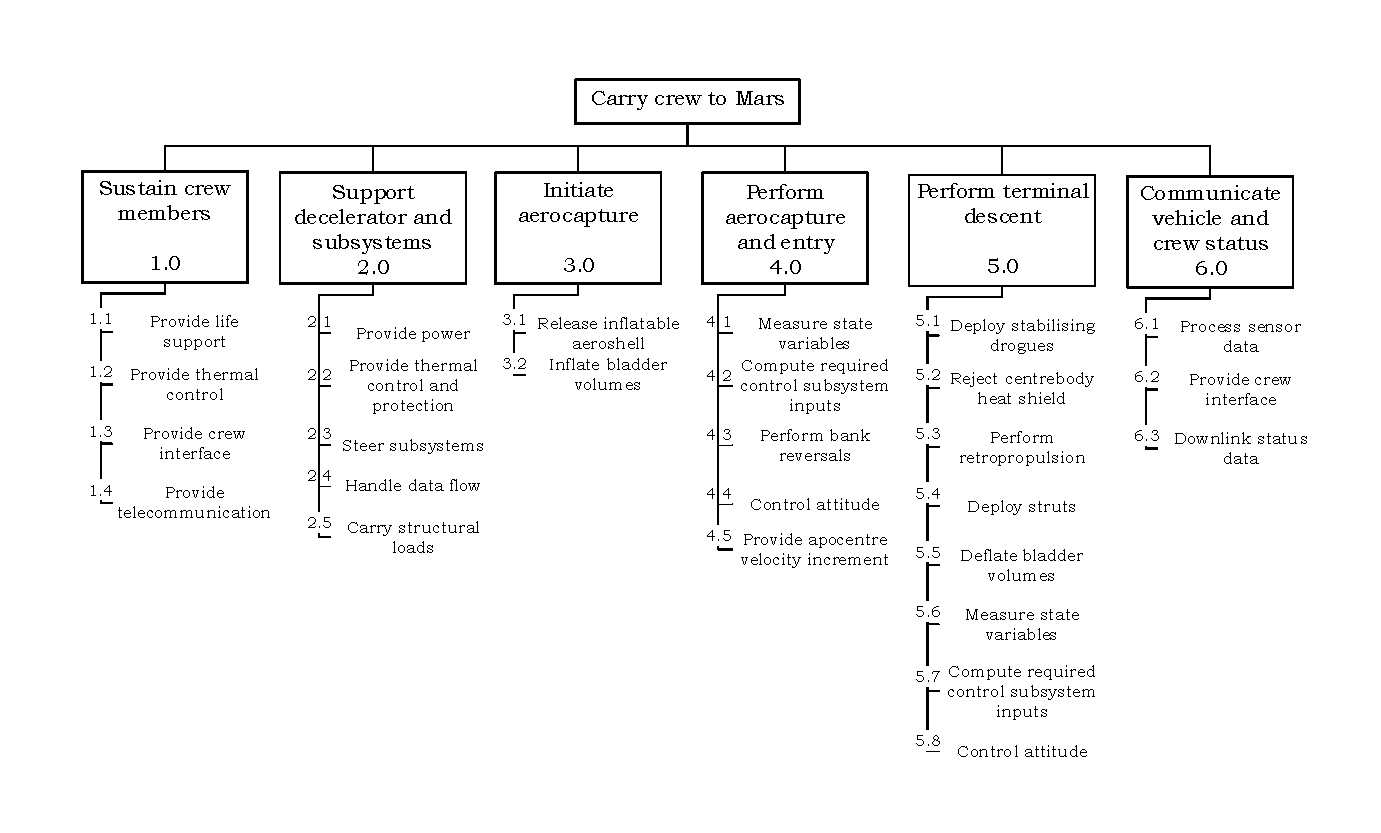
\includegraphics[width=0.95\textwidth]{./Figure/subsystem_breakdown/FBS.pdf}
	\caption{Entry vehicle \acrfull{fbs}}
	\label{fig:fbs}
\end{figure}
Sequencing the functions of the \gls{fbs} in time yields the \acrfull{ffd} in Figure \ref{fig:ffd}. Sequencing of sub-functions 3.1-3.2, 4.0-4.5 and 5.0-5.8 is taken up in the respective sections discussing their design. Sub-functions 1.1-1.4, 2.1-1.5 and 6.1-6.3 are performed continually.
\begin{figure}[h]
	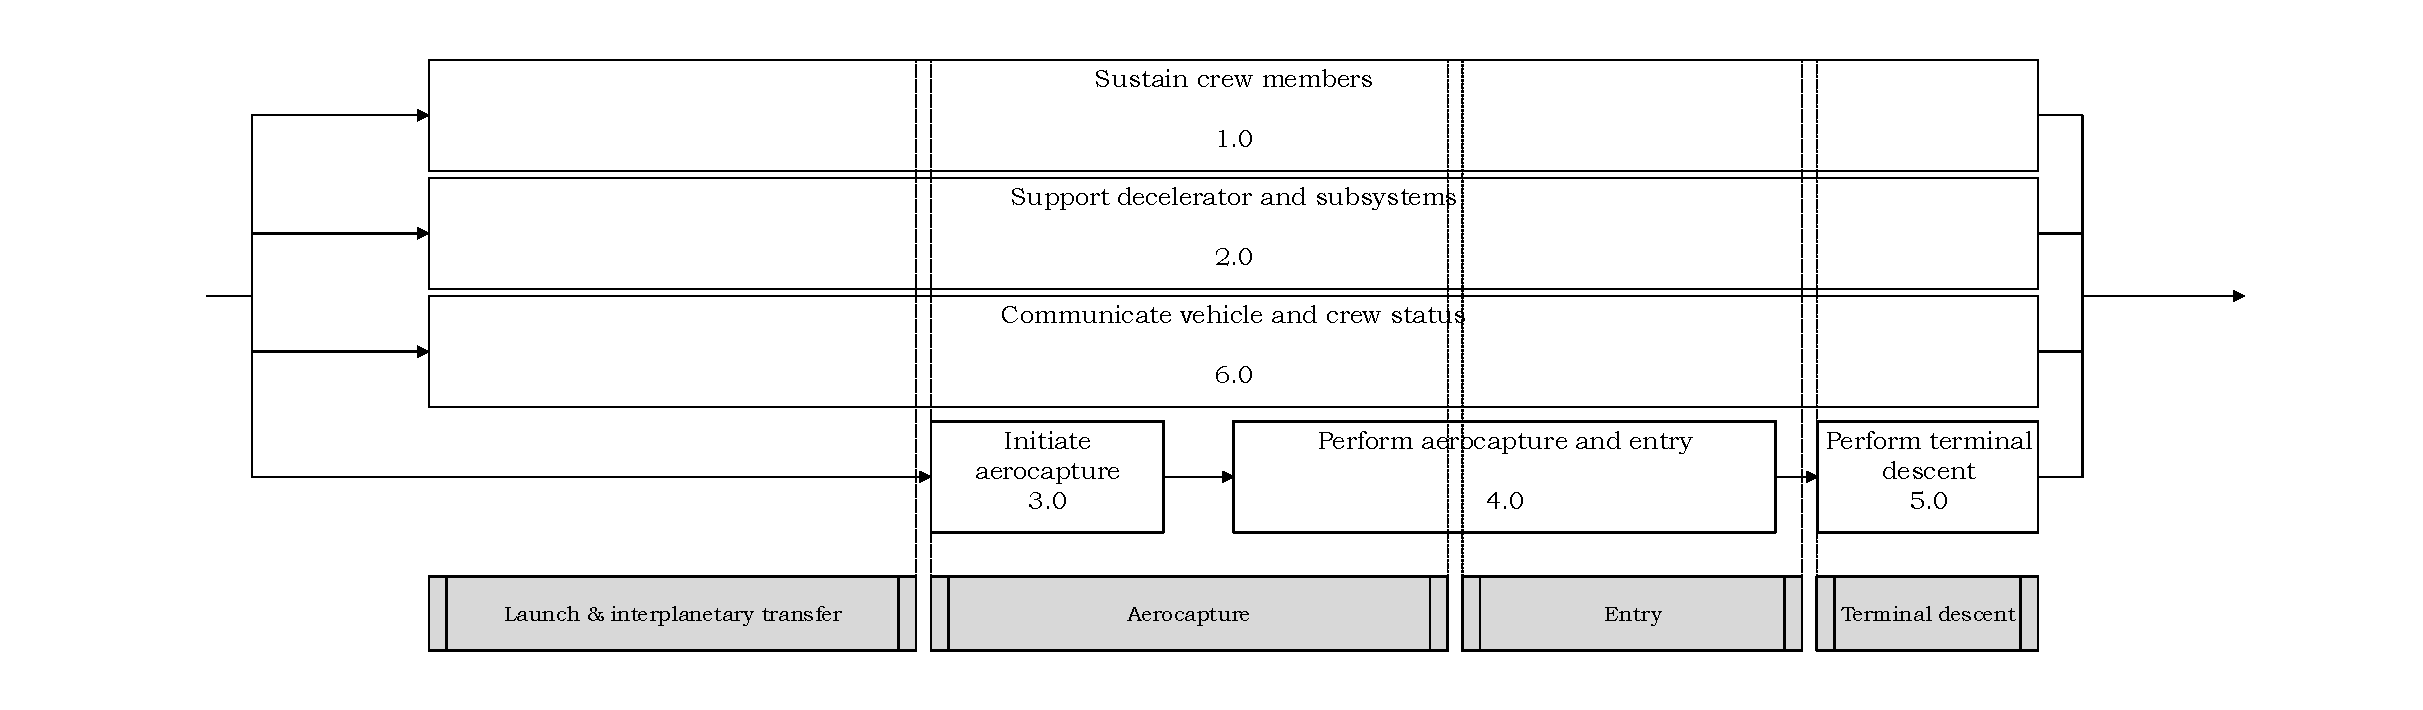
\includegraphics[width=1.00\textwidth]{./Figure/subsystem_breakdown/FFD.pdf}
	\caption{Entry vehicle \acrfull{ffd}}
	\label{fig:ffd}
\end{figure}





\subsection{Subsystem breakdown} \label{sec:subsysbreak}
A tally was made of all the subsystems included in the spacecraft. First a division can be made by distinguishing between the subsystems pertaining to the crew module and those included in the \gls{cia}. This division is shown in Figure \ref{fig:subsystems}. Also shown in Figure \ref{fig:subsystems} are all the subsystems included in the crew module and decelerator.
\begin{figure}[h]
	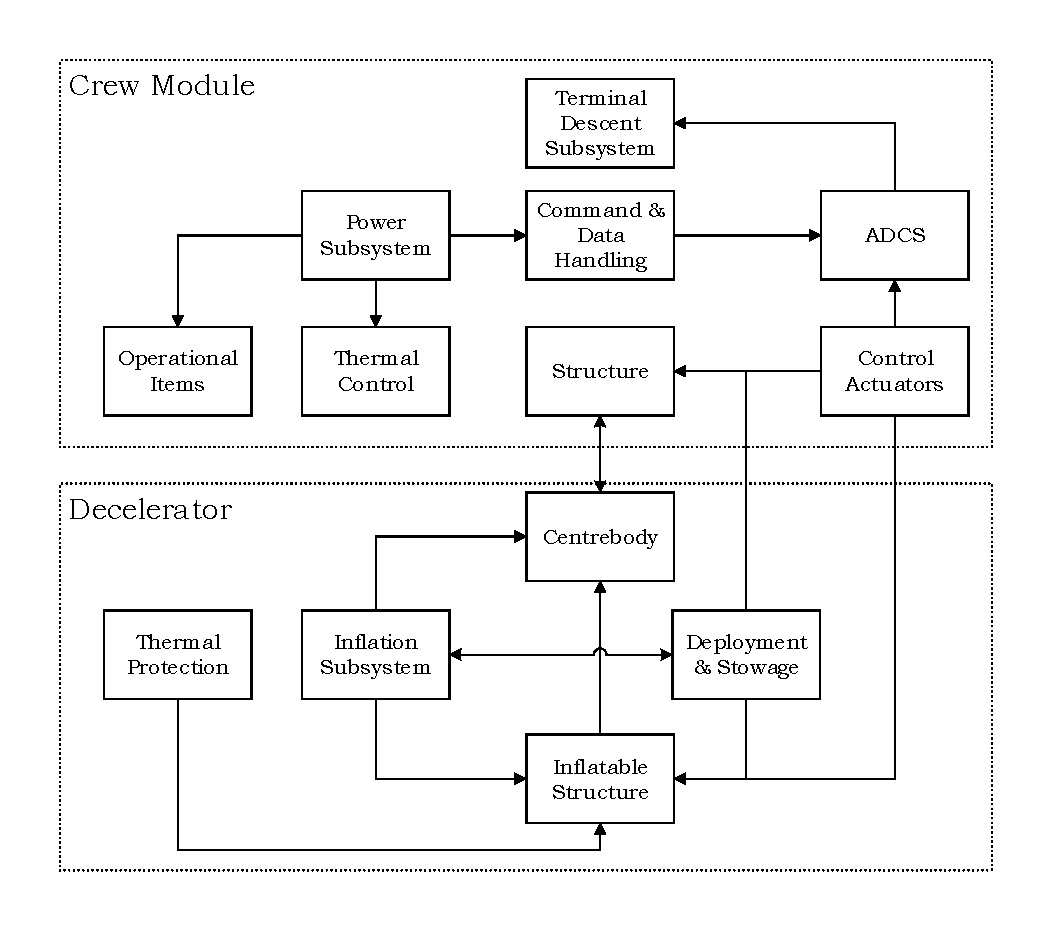
\includegraphics[width=0.95\textwidth]{./Figure/subsystem_breakdown/hardware_structure.pdf}
	\caption{Hardware diagram depicting the primary connections between the subsystems}
	\label{fig:subsystems} 
\end{figure}
%There exist some links between several of the subsystems. The \gls{tps} needs to protect the inflatable structure, centerbody, actuators and crew module. 
%
%** relation tussen inflation system, deployment en inflatable structure **
%
%** relation tussen inflatable structure en centerbody**
%
%** relation betwussen locaties actuators \& type control system (thrusters, flaps, cg offset) **
%
%** relation between actuators \& ADCS van crew module **
%
%** relatie tussen thermal control \& operational items van crew module**
%

As can be seen from Figure \ref{fig:subsystems} connections exist between several of the subsystems, both confined to the decelerator and crew module and between them. In the decelerator the inflation, deployment and stowage systems are closely related with the inflatable structure. The former two are required in order to utilise the stowed inflatable structure to fulfill its mission. The inflation system is located in the centre body. The inflatable structure is stowed against the crew module structure.

While decelerating the \gls{tps} has to protect the inflatable structure from the intense heat produced by aerodynamic forces. %At the same time the control actuators located on the inflatable structures are working to control the attitude of the spacecraft, in conjunction with the \gls{adcs}.\\

The inflatable structure is attached to the crew module structure through the rigid centre body. Control actuators can be attached to both the inflatable and crew module structure. These actuators are managed by the \gls{adcs} which receives inputs from the \gls{cdh}.\\
The power system delivers electrical power to the aforementioned \gls{cdh}, thermal control system and the operational items. At the end of the aerocapture and entry phase the \gls{adcs} provides the attitude control required for the terminal descent system.


\clearpage
\subsection{Technical risks} \label{sec:sysrisk}
A risk map, as can be seen in Table \ref{tab:riskmap}, is made in order to identify which elements and components might pose a risk to the mission. Those risks may cause a decrease in technical performance, scheduling overruns or unpredicted changes in mission costs. The risk elements are first listed in Table \ref{tab:riskmapelements}, after which they are placed inside a risk map. Each of these elements gets assigned a \gls{trl} based on the maturity of the technology that will be used in the corresponding element \cite{NASA2007}. On the horizontal axis the consequence of failure is displayed. The \gls{trl}-classification is shown in Table \ref{tab:trls}.

Next to the risk map, precautions have been taken to prevent an increase in design mass over time. To do so contingency factors are introduced to predict mass increments during the design process. \gls{nasa} has proposed guidelines for contingency factors \ref{tab:riskmap}. As result, in this preliminary design a contingency factor of 20\% is taken into account.

\begin{table}[h]
	\caption[\acrshort{nasa} \acrlong{trl}]{\acrshort{nasa} \acrlong{trl} \cite{NASA2007}}
	\begin{tabular}{|p{0.2\textwidth}|p{0.75\textwidth}|}
		\hline
		\textbf{\acrfull{trl}} & \textbf{Description} \\ \hline \hline
		\gls{trl} 9& Actual system "flight proven" through successful mission operations\\
		\gls{trl} 8& Actual system completed and "flight qualified" through test and demonstration (ground or space)\\
		\gls{trl} 7& System prototype demonstration in a space environment\\
		\gls{trl} 6& System/subsystem model or prototype demonstration in a relevant environment (ground or space)\\
		\gls{trl} 5& Component and/or breadboard validation in relevant environment\\
		\gls{trl} 4& Component and/or breadboard validation in laboratory environment\\
		\gls{trl} 3& Analytical \& experimental critical function and/or characteristic proof-of-concept\\
		\gls{trl} 2& Technology concept and/or application formulated\\
		\gls{trl} 1& Basic principles observed \& reported \\
		\hline
	\end{tabular}
	\label{tab:trls}
\end{table}


\begin{table}[h]
	\centering
	\caption{Risk map elements}
	\label{tab:riskmapelements}
	\begin{tabular}{|c|c|}
		\hline 
		\textbf{Number} & \textbf{Element} \\ \hline \hline
		1 & \acrlong{tps} material \\
		2 & \acrlong{tps} connections\\
		3 & Structural materials\\
		4 & Structural connections\\
		5 & Inflation system \\	
		6 & Deployment mechanism\\
		7 & Decelerator-capsule joints\\
		8 & Aerodynamic shape\\
		9 & Pressure sensors\\
		10 & Bank-control thrusters\\
		11 & \gls{adcs} thrusters\\
		12 & \gls{adcs} reaction wheels\\
		\hline
	\end{tabular}
\end{table}

\begin{table}[H]
	\centering
	\caption{Risk map}
	\label{tab:riskmap}
	\begin{tabular}{|c|c|c|c|c|} % MAKE SURE THAT THE TOTAL WIDTH IS 0.95\textwidth!! (that way its exactly the textwidth.... haha) 
		\hline
		\textbf{\gls{trl} 1} & \cellcolor{green!70} & \cellcolor{yellow!75}  & \cellcolor{red!60} & \cellcolor{red!60}  \\ \hline
		\textbf{\gls{trl} 2} & \cellcolor{green!70} & \cellcolor{yellow!75}  & \cellcolor{red!60} & \cellcolor{red!60} \\ \hline
		\textbf{\gls{trl} 3} & \cellcolor{green!70} & \cellcolor{yellow!75} & \cellcolor{yellow!75} 8 & \cellcolor{red!60}  \\ \hline
		\textbf{\gls{trl} 4} & \cellcolor{green!70} & \cellcolor{yellow!75} & \cellcolor{yellow!75} & \cellcolor{yellow!75} 3 \\ \hline
		\textbf{\gls{trl} 5} & \cellcolor{green!70} & \cellcolor{green!70} & \cellcolor{yellow!75} 2 & \cellcolor{yellow!75} 1, 6 \\ \hline
		\textbf{\gls{trl} 6} & \cellcolor{green!70} & \cellcolor{green!70} & \cellcolor{green!70} & \cellcolor{green!70}\\ \hline
		\textbf{\gls{trl} 7} & \cellcolor{green!70} & \cellcolor{green!70} & \cellcolor{green!70} & \cellcolor{green!70} 4, 5, 7 \\ \hline
		\textbf{\gls{trl} 8} & \cellcolor{green!70} & \cellcolor{green!70} & \cellcolor{green!70} & \cellcolor{green!70} \\ \hline
		\textbf{\gls{trl} 9} & \cellcolor{green!70} & \cellcolor{green!70} 9, 12 & \cellcolor{green!70} 11 & \cellcolor{green!70} 10  \\ \hline
		& \textbf{Negligible} & \textbf{Marginal} & \textbf{Critical} & \textbf{Catastrophical} \\ \hline
	\end{tabular}
\end{table}








\section{Crew module design and sizing}\label{ch:crewmod}
It is essential that the crew module is designed and sized for the following purposes. Firstly, it is a prerequisite to size control mechanisms as the crew module is a dominant contributor to mass moments of inertia by its large mass. Secondly, it allows determination of the number of crew members to be taken on board and thereby to investigate advantages of an inflatable aerodynamic decelerator over the conventional rigid solution, such as Orion. Thirdly and most importantly, it is required to yield a full mission description.

To this end, crew module subsystems are designed and sized at a preliminary design level in section \ref{sec:crewsubsys}. Each subsystem is given and accompanied by mass, power and volume budgets. The latter two allow for packaging of the crew module to effect a \gls{cg} location that minimizes required control system activity. Crew module subsystem integration is described in section \ref{sec:crewpackaging}. The crew module configuration is carried through in the final design as an input for the control system as well as to harmonize a design that integrates crew module and decelerator.

\subsection{Subsystem design and sizing} \label{sec:crewsubsys}
The \acrfull{adcs}, \acrfull{cdh}, operational items (including life support), capsule structure, thermal control and power and the terminal descent system are key components of the crew module. A basic sizing and design follows hereafter.

\subsubsection{Attitude determination \& control} \label{subsec:adcs}
The general objective for the \gls{adcs} is to monitor the attitude of the spacecraft and perform corrections if needed. The operation period of the \gls{adcs} can be divided into two phases, the interplanetary phase and the Mars approach phase:
\begin{itemize}
\item During the interplanetary flight the \gls{adcs} keeps the attitude as required to point the solar arrays toward the sun, points the thrusters in the desired direction and to ensure nominal trajectory is followed.

\item During the Mars approach phase the \gls{adcs} should adjust the attitude to the entry attitude and compensate for possible disturbances (i.e. inflation of the \gls{hiad}) to adhere to the nominal trajectory.
\end{itemize}
\paragraph{Sensors} Sensors are needed to determine the attitude. How accurate the sensors need to be depends on the required accuracy from different subsystems. For instance a high gain antenna requires a higher accuracy. 

\subparagraph{Star trackers}
Star trackers work by taking pictures of the stars and comparing them to an internal catalogue. They are the most accurate for pointing \cite{CarlChristianLiebe1995}. However they do not work if the spacecraft is rotating too fast, so an additional rough estimate is needed \cite[p. 584]{Wertz2011}. 

The mass of star trackers is in the order of $0.1 \left[kg\right]$. The required operating temperature range is $-30 \left[^\circ C\right]$ to $+50 \left[^\circ C\right]$. The average power consumption is less than $0.5 \left[W\right]$.\footnote{URL: \url{http://www.sinclairinterplanetary.com/startrackers} Accessed: 11-06-2015}

\subparagraph{Gyroscope}                        
Gyroscopes can be used to provide the attitude determination for the initial stabilisation. There are different kinds of gyroscopes: Mechanical, optical and so-called \gls{mems}. The latter one is relatively new, and is widely used in mobile phones. 

\subparagraph{Accelerometers}                        
Accelerometers are a crucial element for control in the aero capture and final \gls{edl} of the entry vehicle. They allow for determination of control model parameters. More details with respect to this are given in Section \ref{subsec:controlsys}.

\paragraph{Attitude control}
During the interplanetary flight the space craft will encounter disturbance torques. To prevent attitude changes, these disturbances must be counter acted. Although the thrusters used during the entry stage of the mission could be used for this, these are only capable of providing bursts of angular momentum. Instead, reaction wheels will be used. These momentum wheels continuously store the disturbance torques. Once they are spun up to their rated angular speeds, they must be unloaded using thrusters. Taking the Mars Reconnaissance Orbiter \cite{You2007} as a reference case for the required momentum storage and unloading, and scaling these values to be more representative of crew module during interplanetary flight, an angular momentum storage capacity of $\gls{sym:l} = 1000 \left[N \cdot m\cdot s^{-1}\right]$ and a momentum unloading $\Delta\gls{sym:V}$ of $5 \left[m\cdot s^{-1}\right]$ is needed. Assuming the reaction wheels have a diameter of 0.5 $[m]$ and spin to a maximum of $500 \left[rad \cdot s^{-1}\right]$ each wheel will have a mass of roughly $65 \left[kg\right]$. For a $10 000 [kg]$ crew module using MR-104G thrusters, a $\Delta\gls{sym:V}$ of $5 \left[m\cdot s^{-1}\right]$ corresponds to a propellant mass of roughly $20 \left[kg\right]$ per Tsiolkovsky's rocket equation. 

\subsubsection{Command, data handling and telemetry} \label{subsec:cdh}
\acrfull{cdh} and telecommunications form an integral part of the avionics system. These perform four functions: flight and vehicle control, data processing, human interfacing and communications \cite{Eger2008}. This requires a direct link to the \gls{adcs} module, a link to the telecommunications network and a link to on-board display for crew members. These are illustrated in Figure \ref{fig:cdhflow}

\begin{figure}[h]
		\centering
		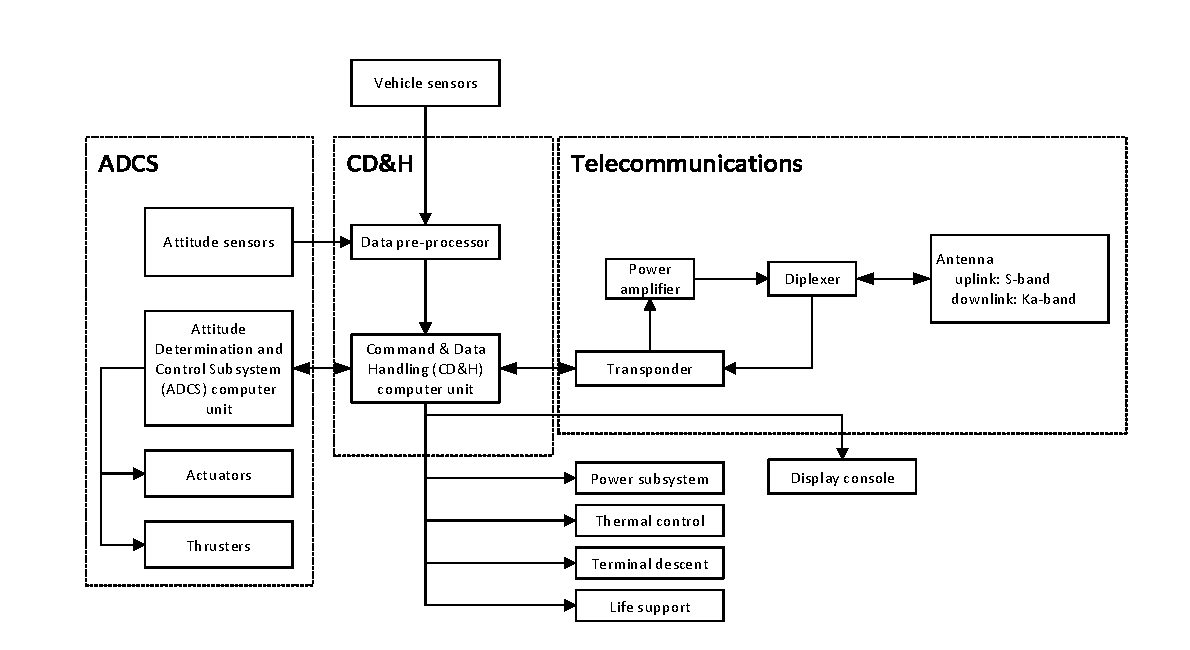
\includegraphics[width=0.95\textwidth]{./Figure/CrewModule/CDH.pdf}
		\caption{Communication flow}
		\label{fig:cdhflow}
\end{figure}

Data processing is performed as follows. Data is first filtered, then analysed to see if reactions are required and in case reactions are required put through to the relevant effectors (subsystems) and critical system information communicated to the ground station via the Ka-band (see section \ref{sec:groundop}). Modulation is performed in the transponder by \gls{bpsk} on the carrier and subcarrier (modulating the carrier) and \gls{qpsk} on the carrier, similar to the Mars Reconnaissance Orbiter mission \cite{Taylor2006}.

For its integral part, it is key that the system is redundantly equipped to ensure adequate system reliability. To this end, cabling is redundant and safety-critical processing tasks are performed by self-checking pair processors, following their application in Orion \cite{Eger2008}. These self-checking pair processors observe and compare the activity of their partner to identify faulty behaviour. 

Antennas used can be extracted from a reference mission to Mars, for example the Mars Reconnaissance Orbiter \cite{Taylor2006}. This mission had relatively high scientific return communications and used a $3$ [$m$] diameter high gain antenna and two low gain antennas. The communication system for this mission was remarkable because it was able to send data back to Earth more than ten times faster than previously conducted missions. Such a high return would be highly beneficial for the manned mission at hand to maximize ground surveillance possibilities and accurate monitoring. It similarly used Ka-band communication for downlink. To this end, the communication system is deemed a good reference system for use in the mission at hand.

The mass of the \gls{cdh} subsystem is extrapolated from that in the Mars Odyssey mission by scaling with the ratio of masses. For a $11.1$ [$kg$] \gls{cdh} subsystem mass in the 376 [$kg$] Mars Odyssey\footnote{URL:\url{http://mars.nasa.gov/odyssey/mission/spacecraft/parts/command/}. Accessed: 11-06-2015}, this translates to nearly $300$ [$kg$] on the $10,000$ [$kg$] entry vehicle at hand. This telecommunications system had a mass of $108$ [$kg$], which is not scaled since the sizing thereof is not deemed mass-dependent. Taking into account a contingency for the larger crew module and more demanding mission at hand as well as the roughness of the estimates, the \gls{cdh} and telecommunications mass is estimated at $530$ [$kg$], thus taking a $30$ $\%$ contingency into account. In addition, cabling requires additional contingency, taken to be $10$ $\%$ and a mass of $53$ [$kg$].


\subsubsection{Operational items} \label{subsec:crewop}
In this section the operational items are sized. This can be summarised as the mass needed by the astronauts to stay alive in the crew module during the mission. For this purpose the paper by Tito et al \cite{tito2013} has been used. In this paper the operational items are called \textcolor{red}{GLS} Environmental Control and Life Support System (ECLSS). First the method for estimation is described with its assumptions. Followed by the results of the estimation.

\paragraph{Estimation method}
\label{par:operationalest}
The mass of the \textcolor{red}{ECLSS (GLS)} is primarily driven by the crew size and mission length. The \textcolor{red}{ECLSS (GLS)} is divided into subsystems: Air Management, Thermal and Humidity Management, Water Management, Waste Management, Human Accommodation, Food Preparation and Storage. Each of these subsystems can be subdivided into components. Examples of these are a water heater or packed food in the Food Preparation and Storage. It is evident that some components scale with the keydrivers and others do not. For example, adding a crew member does not necessitate an extra water heater, but it does require extra packed food. 


Taking this into account the mass has been divided into two components. A basic system mass which scales with crew size and the consumable mass that scales with crew size and mission length.





afasasfasf
\paragraph{Results}
By using the methods from section \ref{par:operationalest} the results of table \ref{tab:operationalest} were obtained.
The masses associated with operational items can be split up into two sections: Basic system mass and consumables mass. Basic system mass consists of the systems concerning crew well-being and life support, such as: Oxygen scrubbers (not including oxygen), atmospheric control systems and food preparation systems. Consumables mass is concerned with items such as oxygen, food, water and personal provisions.
\begin{table}[h]
	\centering
	\caption{Obtained masses and volumes of basic system \& consumable items}
	\begin{tabular}{|p{2cm}|p{2cm}|p{2cm}|p{2.5cm}|p{2.5cm}|}
		\hline
		\textbf{Crew members} & \textbf{Basic system mass $[kg]$} & \textbf{Basic system volume $[m^{3}]$} & \textbf{Consumables mass per day $[kg]$} & \textbf{Consumables volume per day $[m^{3}]$} \\ \hline \hline
		1 & 1,800 & 4.88 & 3.2 & 0.018 \\
		2 & 2,500 & 6.78 & 6.4 & 0.036 \\
		3 & 3,200 & 8.68 & 9.6 & 0.054 \\
		\hline
	\end{tabular}
	\label{tab:operationalest}
\end{table}
It can be seen from table \ref{tab:operationalest} that both the basic system and consumables mass scale with the number of crew members. By using linear extrapolation the mass and volume associated with crew members higher than three can be determined. These are shown in table \ref{tab:crewmemberops} for a mission time of $100$ days.\\

\begin{table}[h]
	\caption{Total mass and volume associated with operational items for varying crew numbers}
	\begin{tabular}{|c|c|c|}
		\hline
		\textbf{Crew members} & \textbf{Operational items mass $[kg]$} & \textbf{Operational items volume $[m^{3}]$}\\ \hline \hline
		1 & 2,120 & 6.69\\
		2 & 3,140 & 10.40\\
		3 & 4,160 & 14.11\\
		4 & 5,180 & 17.82\\
		5 & 6,200 & 21.53\\
		6 & 7,220 & 25.24\\ \hline
	\end{tabular}
	\label{tab:crewmemberops}
\end{table}

\subsubsection{Capsule structure} \label{subsec:crewstruc}
The structure of the crew module serves the important function of connection all the individual subsystems of the crew module and moreover connects with the \gls{hiad}. The main scope of the design described in this report lies within this \gls{hiad}. New advances from for example the currently being developed and Orion mission are therefore not considered. The Orion capsule can already be considered state of the art and is in a large amount representative for the crew module design.

A schematic layout as for example also used in the Orion spacecraft\footnote{URL: \url{http://www.spaceflight101.com/orion-spacecraft-overview.html}, Accessed 11 June 2015 }, features a Aluminium grid structure. This structure encloses the pressurised volume inhabited by the astronauts. The grid structure allows for easy attachment of the individual subsystems. Subsystems which require pressurisation, typically those involving the astronauts can be placed within in this shell, whereas the systems that do not require pressurisation are placed on the outside of this shell. A more detailed analysis on where each of these individual subsystems are placed is discussed in Section \ref{sec:crewpackaging}.


A full estimate of the structural mass is only to be provided in later design phases. More detailed structural estimates are typically provided by detailed \gls{cad} models and \gls{fem} models \cite{Wertz2011}. A rough estimate can be provided on the basis of previous reference missions. \gls{nasa}'s Orion mission is again of primary interest as it also features astronauts. Some differences with respect to the structural elements thereof can however be noted:

\begin{itemize}
\item Orion incorporates an integrated heat shield and structure
\item Orion features a backshell, not required for the inflatable aeroshell by its larger deployed diameter
\end{itemize}

In the design at hand the heat shield structure is incorporated in the \gls{hiad}. The crew module is merely connected to this \gls{hiad} of which the latter is designed in more detail in the remaining chapters of this report. Due to the implementations of the \gls{hiad} a additional backshell structure is also no longer required. The back shell normally functions a protection against thermal loading which moves sideways along the body. Using the large frontal of the inflatable this is prevented, denoting one of the advantages of using a inflatable structure \cite{Hughes2005}. The crew module structure should however also be sized considering , and may as such not be too tall and may feature a tapered end such that the crew module is not exposed to thermal loading passing the \gls{hiad}.

For this reason the heat shield carrier structure of around $1500 \left[kg\right]$ \cite{Ainsworth2014} is not taken into account into the mass estimate of the structure. A total structural mass for manned re-entry vehicles lies at around 30\%. The manned Apollo mission featured a 31\% structural mass fraction \footnote{URL: \url{http://braeunig.us/space/specs/apollo.htm}, Accessed 11 June 2015} including a heat shield structure. Extrapolating this value, with a $9000 \left[kg\right]$ crew module mass yields a structural mass of $1300 \left[kg\right]$, excluding the heat shield structure. This is in line with values suggested by Wertz et al. \cite{Wertz2011}. Taking into account a 30\% mass contingency factor yields a final structural mass estimate of around $1700 \left[kg\right]$. A similar mission featuring a descent towards Mars from $7 \left[km \cdot s^{-1}\right]$ has a structural mass of $517 \left[kg\right]$ on a dry mass of $2863 \left[kg\right]$ including contingency factors\footnote{URL: \url{http://www.nasa.gov/pdf/458812main\_FTD\_AerocaptureEntryDescentAndLanding.pdf} , Accessed 11 June 2015 }. Scaling this value yields a similar mass estimate of around $1800 \left[kg\right]$. 

The connection between the crew module and the \gls{hiad} is taken into account in the capsule structural mass estimate of $1300 \left[kg\right]$.

\subsubsection{Capsule thermal control} \label{subsec:crewthermalcontrol}
Where the \acrfull{tps} is used to protect the crew module from excessive heating during re-entry, the \acrfull{tcs} is used to keep other subsystems in the crew module within their operating temperature limits. It is assumed that re-entry phase does not impose extra requirements on the \gls{tcs} as it is completely covered by the \gls{tps}. Note that this only holds when the angle of attack ($\alpha$) is low enough such that the crew module stays out of the wake. Furthermore, the paper used in the mass estimation for the operational items already assigns a mass for the thermal control withiasd


startracker -30,+50. 

asd



\subsubsection{Capsule power} \label{subsec:pwer}
In order to succefully operate the mission during transfer and the \gls{edl} phase. \\

Piece on the items that the power subsystem needs to drive.\\

Small trade-off / considering possible options for power generation. (solar arrays, batteries, reactor)\\

Power during EDL.\\

conclusion on mass and volume.\\







\subsubsection{Terminal descent system} \label{subsec:crewtermdescent}
Terminal descent takes place in the following sequence:
\begin{enumerate}
\item [HEAT SHIELD EJECTION]
\item At this altitude, retropropulsion is activated and the thruster provides the decelerating force in combination with the inflated aeroshell.
\item At an altitude of 50 [$m$], struts are partially deployed from their stowed position such that the pads rest above the inflatable. At the same time, the vent in the inflation system is opened and inflatable bladders deflate. Upon full deflation, measured by pressure transducers in the inflation system, the struts deploy further such that the pads are level with but below the thruster nozzle exit and achieve a roughly 90 [$deg$] inflatable half-cone angle.
\item The thruster is then deactivated and the crew capsule lands on the inflatable, on which the landing gear pads rest.
\end{enumerate}
Retropropulsion is used for the beneficial aerodynamic interaction with a \gls{hiad} \cite{xxx}, effecting a required specific impulse that is twice as low as otherwise. This effects a smaller propellant mass required. The inflatable is not rejected, but rather deflated, because rejection would require a separation mechanism to prevent interference with the crew capsule. Deflation does induce, however, the risk that it is not performed reliably. In such a case, a risk mitigation plan could be deliberate puncturing of the inflatable bladder volumes in order to deflate it.

[THRUSTER MASS]


The terminal descent system, as described in Section \ref{sec:terminal}, consists of the thruster system that decelerates the spacecraft from Mach 5 at 10 [km] height to zero velocity at a height of 0 [km]. The thruster should be placed in the centerbody and pointed in the forward direction, such that the positive interaction between aerodynamics and the thruster plume is made use of. The total thruster mass, including fuel is estimated to be approximately 1300 [kg], based on extrapolation of .................
The thruster mass is estimated to be 470 [kg], based on a 3g deceleration and using an empirical relation\cite{Christian2006}. This leaves approximately 930 [kg] for the fuel. Assuming the density of the fuel at 1000 $[kg\cdot m^{-3}]$\footnote{\url{http://en.wikipedia.org/wiki/Liquid-propellant_rocket}. Accessed: 11-06-2015} means the required volume for fuel is 0.93 [$m^3$].






\subsection{Crew module configuration} \label{sec:crewpackaging}
Space allocation of the subsystems described in the previous section, as well as crew members, is performed with the goals of:
\begin{itemize}
\item Accommodating subsystems necessary to support interplanetary flight and entry
\item Providing crew members with a habitable volume and operational items to support a flight duration of approximately 100 days
\item Keeping the axial position of the \gls{cg} forward to lower pitch stability and alleviate pitch control performance in the final mission phase
\item Allowing for packaging freedom in achieving a static lateral \gls{cg} offset for creating an asymmetric lifting shape
\end{itemize}
To this end, the crew module is packaged as depicted in Figures \ref{fig:axview} and \ref{fig:topview}. 

The top part is required to contain drogues to stabilize the entry vehicle in its final descent phase. Four drogues are placed to incorporate redundancy and provide
a symmetric configuration, to prevent excessive tilting during final descent. Moreover, the top part contains the foldable solar arrays required to generate power required during interplanetary transfer. These are placed in the top part to prevent interference with the flow during entry on one hand and with thrusters and the stowed inflatable before entry on the other hand. A high-gain antenna of adjustable attitude on a boom enables communication during all mission phases. A first-order estimate for the length of this upper part is $0.2$ $[m]$, based on the Orion configuration\footnote{URL:\url{http://www.spaceflight101.com/orion-spacecraft-overview.html}. Accessed: 15-06-2015}.

Crew members are located in the next part, a habitable volume to their availability that is dictated by the performance limit for a three-month mission duration as 11 $[m^{3}]$ per crew member \cite{Rudisill2008}. The diameter of the habitable volume is 4.0 $[m]$, thereby less than vehicle maximum diameter to accommodate four propellant tanks, one per quadrant, that allow intertank propellant transfer to shift the lateral \gls{cg} position. The tanks are sized on the basis of the total required propellant and provide propellant for both the reaction control thrusters and main thruster. The length of this part follows from the habitable volume and depends on the number of crew members.

Operational items are located below, within reach of crew members. These are placed at this location because of their relatively high mass and therefore contribution to the axial \gls{cg} position. The total volume occupied follows from Table \ref{tab:crewmemberops}. On one hand these operational items include relatively dense products, foremostly the life support systems, and less dense products in the form of food and other supplies. Arranging these items asymmetrically allows for a lateral \gls{cg} offset, most notably considering the depleted supplies of food at the end of interplanetary transfer while life support system mass remains intact. The length of this part follows from the required volume for operational items.

The last part of the crew module contains four struts for touchdown, packed symmetrically. The struts are arranged about the batteries required to provide power during entry, where solar panels are stowed, a nitrogen tank for inflation of the inflatable aeroshell and the main thruster to provide in-plane velocity changes. The length follows from estimates for the strut required volume based on the Apollo landers and is an estimated 1.0 $[m]$. 

The last part contains the thruster nozzle, closed off by a heat-resistant end-cap during entry, and the attachment rings for the inflatable decelerator. It is detachable from the main body and thereby does not contain any other subsystems. The length of this part is mainly dictated by the shape of the inflatable and where it attaches to the centerbody.

\begin{figure}[h]
		\centering
		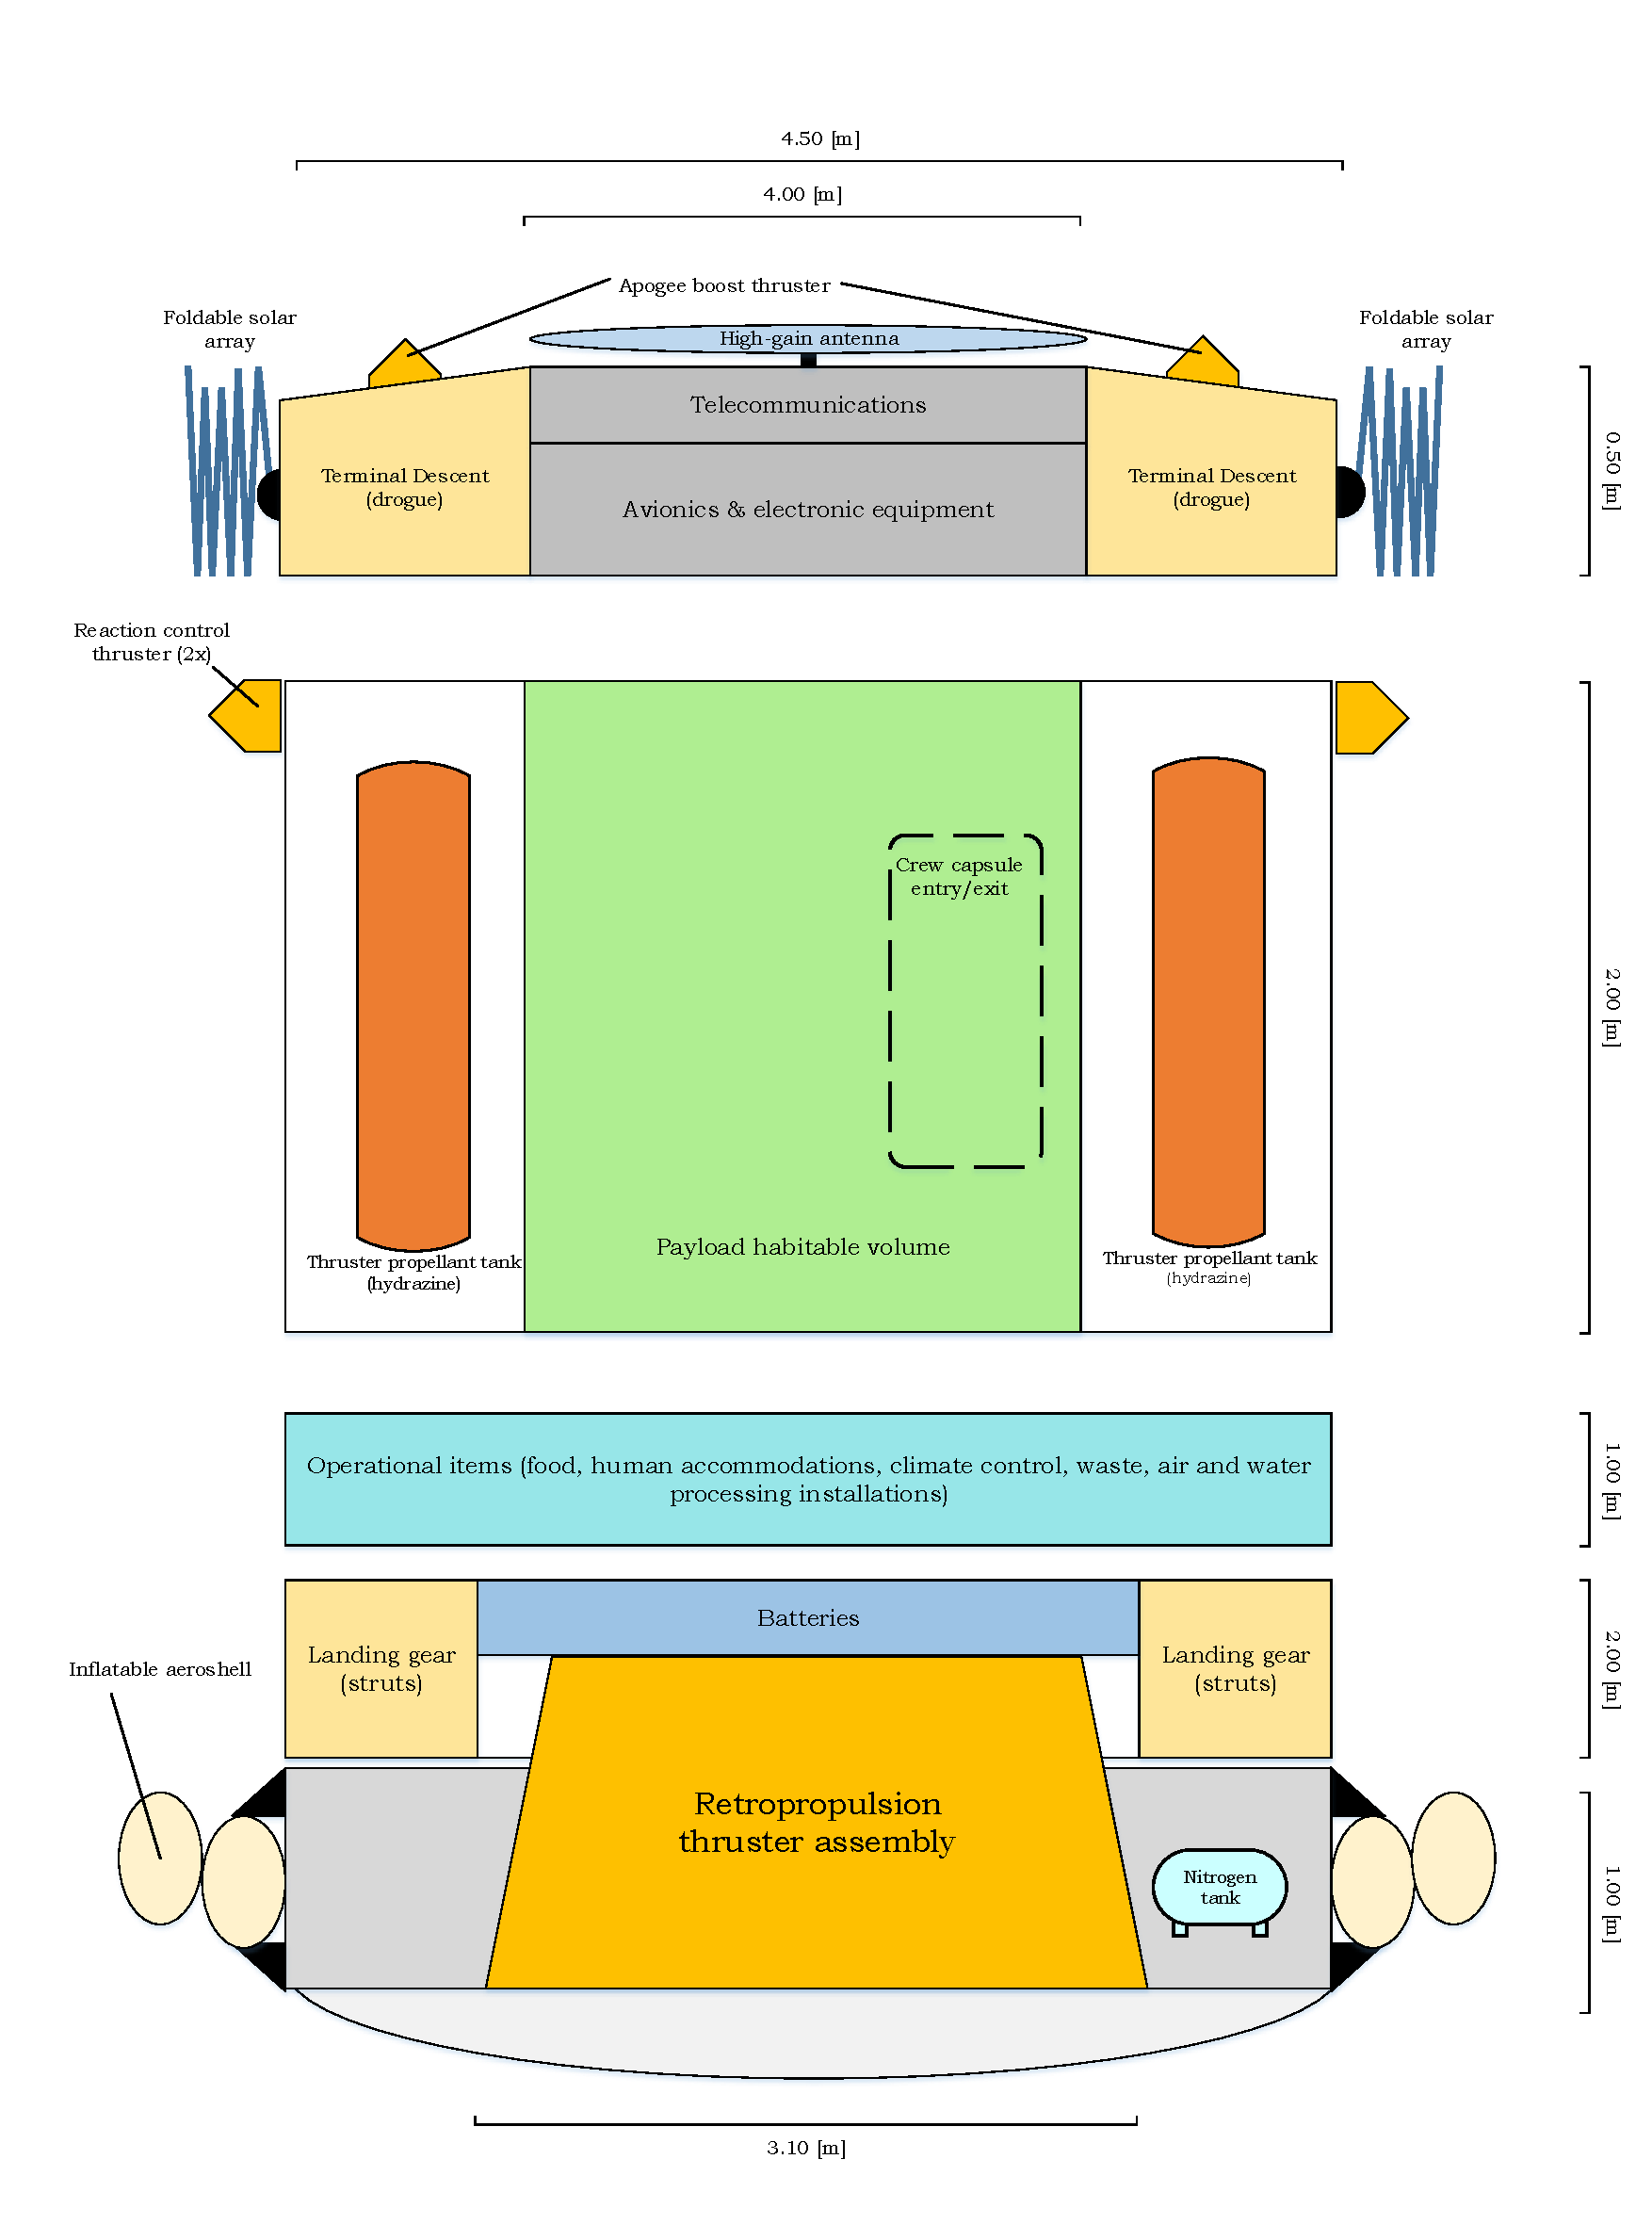
\includegraphics[width=0.95\textwidth]{./Figure/CrewModule/Axialview.pdf}
		\caption{Axial view of crew module lay-out}
		\label{fig:axview}
\end{figure}

\begin{figure}[h]
		\centering
		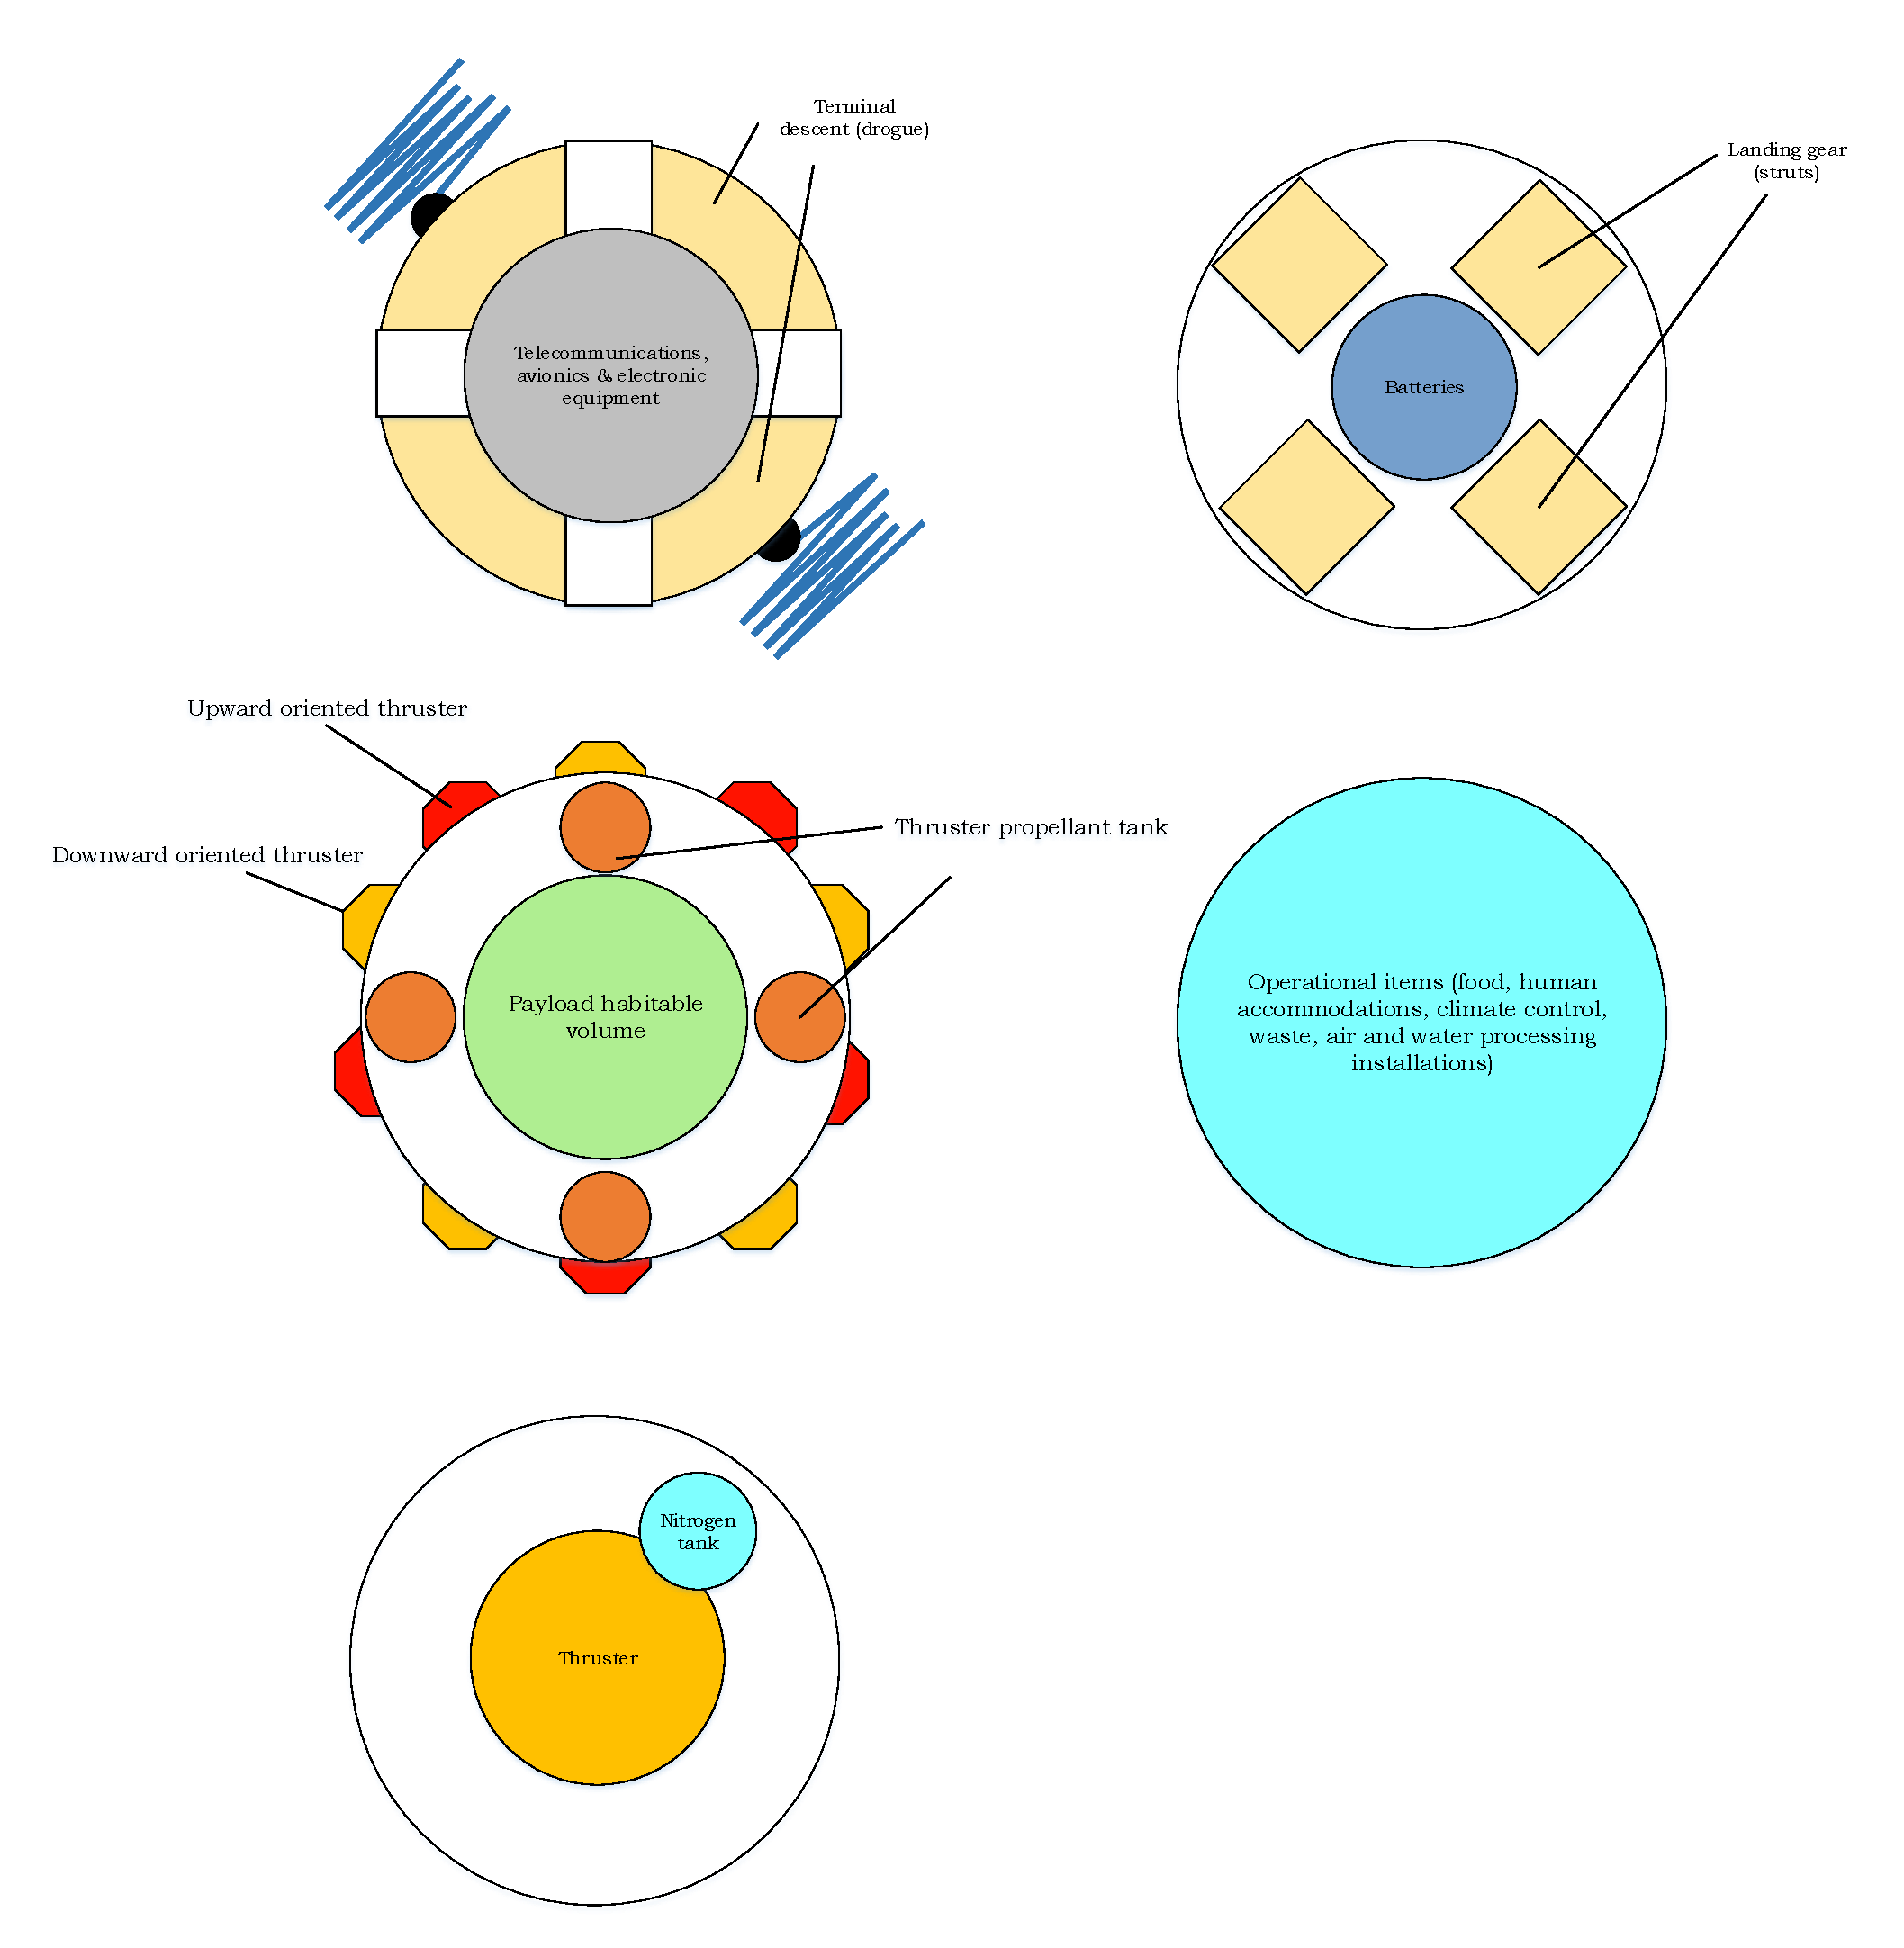
\includegraphics[width=0.95\textwidth]{./Figure/CrewModule/TopviewV2.pdf}
		\caption{Top-down view of crew module lay-out}
		\label{fig:topview}
\end{figure}





\section{Design parameters and tool analysis}\label{cha:designpar}
It is essential for the iterative design process that the design sensitivity is investigated. This sensitivity is quantified by tools for trajectory, thermal structural and aerodynamic analysis. These tools are complemented by a control system tool for the purpose of control system design and sizing. The description of these tools is given in Section \ref{sec:designtools} and their output in Section \ref{sec:designsens}.

\subsection{Design tools} \label{sec:designtools}

\subsubsection{Trajectory analysis}\label{subsec:orbittool}
\paragraph{Input and output}
As input the tool requires the entry velocity, flight path angle at the boundary of the atmosphere, an aerodynamic model (\gls{sym:CL} and \gls{sym:CD} as a function of \gls{sym:alpha}), an \gls{sym:alpha}-profile (changes in the angle of attack during the aerocapture and entry), and a \gls{sym:mu} profile (changes in the bank angle during the aerocapture and entry).

As output the trajectory tool can generate important parameters at each moment in time. The most important parameters are: location (\gls{sym:Rv}), acceleration $\left(\gls{sym:acc}\right)$, dynamic pressure $\left(\gls{sym:q}_{\infty}\right)$, velocity $\left(\gls{sym:Vv}\right)$, Mach number $\left(\gls{sym:M}\right)$, atmospheric temperature $\left(\gls{sym:T}_{\infty}\right)$ and atmospheric density $\left(\gls{sym:rho}_{\infty}\right)$.

\paragraph{Assumptions}
 \label{sec:astroassumption}
 Some of the assumptions have a big impact, these are the primary assumptions. There are, however, also some assumptions that have a negligible effect on the results. These are the secondary assumptions.
 
 \subparagraph{Primary assumptions}
 \begin{itemize}
 \item All atmospheric properties only vary with the height above \gls{mola} and not with longitude, latitude or time. These variations are shown in Appendix \ref{app:atmos}. 
 \item All trajectories are assumed to only occur in the equatorial plane. This means that the latitude is always $0 \left[deg\right]$. Changing the latitude will have a big impact on the relative speed of the Martian atmosphere.
 \item The gravitational pull is assumed to only vary with the height above \gls{mola}. The gravitational field of Mars is however not uniform over longitude and latitude, this will induce errors in the trajectory as gravity is one of the major forces in the analysis.
 \item The bank reversals needed for bank control are assumed to be instantaneous.
 \end{itemize}

 \subparagraph{Secondary assumptions}
 \begin{itemize}
 \item The spacecraft is assumed to only feel a gravitational pull from Mars. It is thus assumed that there is no gravitational pull from the sun, any other planet or the Martian moons.
 \item The atmosphere stops at an altitude of 400 $\left[km\right]$. At this point the atmosphere is negligibly thin, expanding the atmospheric model would not contribute to the results.
 \item The effect of other disturbances i.e. solar radiation is neglected.
 \end{itemize}

\paragraph{Analysis method}
The orbit can be divided into two different parts, one part is the pass through the atmosphere and the other is outside of the atmosphere. In the first part, there are three forces working on the spacecraft: Lift, drag and gravity. In the second part there is only the gravitational force.

The part outside the atmosphere is simplified by using the Kepler equations of orbital motion to determine the position of the spacecraft over time.

The atmospheric properties are determined using the NASA software \gls{marsgram}. The software generates data based on equations for atmosphere properties and incorporates the high amount of dust on Mars, which has a big effect on the absorbed radiation heat from the sun. From this model the average atmospheric properties are used to determine the aerodynamic forces. All data used from \gls{marsgram} is shown in Appendix \ref{app:atmos}. 

Using the aerodynamic forces combined with the gravitational pull from Mars the accelerations are calculated. These accelerations are integrated twice to obtain the velocity and the location.

\paragraph{Limitations}
The tool is mainly limited by the 1D implementation of the atmospheric properties and gravity model. This means that no variations of the atmosphere over longitude, latitude or time are considered. It is recommended to implement the full atmospheric model in later stages of the design. The use of a numerical simulation only introduces a small error. The full verification and validation are done in Appendix \ref{sec:VandVtraj}.

\subsubsection{Aerodynamic analysis}\label{subsec:aerotool}



\paragraph{Important parameters}\label{sec:aeroparams}
 The following parameters were determined to have a significant influence on te performance of the vehicle:

\begin{itemize}
	\item{Lift. As detailed in Section \ref{subsec:orbitsens}, the vehicle requires a lift vector to provide flight path control. A larger lift vector provides an increase in flight path control.}
	\item{Drag. The vehicle decelerates purely on atmospheric drag. An increase in drag will decrease the required time for aerocapture and entry and provides greater flexibility in terms of the path through the atmosphere.}
	\item{Lift-to-drag ratio. The lift-to-drag ratio is an indication of the freedom in the selection of the orbital trajectory. A higher lift-to-drag ratio will provide greater flexibility.}
	\item{\gls{sym:cm-alpha}. The derivative with respect to angle of attack of the moment coefficient is a measure of the stability of the vehicle. }
	\item{\gls{cg} offset}. The \gls{cg} offset at a given angle of attack required to cancel the moment generated by the vehicle at that angle of attack. It is a measure of the control effort required to trim the vehicle. 
	\item{Heat flux. For a given flight condition, the heat flux in the stagnation point depends only on the vehicle geometry.  }
\end{itemize}


\paragraph{Shape sensitivity} \label{sec:aerooptima}
Obtaining favourable characteristics of the aerodynamic shapes requires understanding of the influence of shape parameters on the performance of the design. To this end, firstly an analytical approach is taken. After that, conclusions can be made about different aerodynamic shapes. The optimisation tool is used afterwards to generate shapes that are optimised for certain design parameters, such that the conclusions based on the analytical knowledge can be verified.

In Figure \ref{fig:CLCD-incidence}, the lift and drag performance as well as the lift-to-drag ratio of a flat plate in a free stream is given. Since Newtonian flow theory is based on the assumption that pressure only depends on the local body incidence angle, this plot can be used to deduce performance of a given shape. As can be seen in the plot, a vehicle with a high drag has most of its surface perpendicular of the flow.

\paragraph{Lift}
A high lift is achieved by having large parts of the shape under an incidence angle of 35 $\left[deg\right]$. An axisymmetric shape does not create lift at zero angle of attack, since every radial part of the shape cancels all non-drag forces out. Skewness of the shape, such as portrayed in Figure \ref{fig:skewnessplot}, can be used to create lift at zero angle of attack: a larger part of the surface is inclined upwards than downwards, meaning the skewed shape generates a downward lift. Using skewness instead of an axisymmetric body at a high angle of attack may help to prevent the shock wave from hitting the payload module.

\paragraph{Drag}
Maximum drag is created by having large parts of the shape perpendicular to the flow. This follows directly from Figure \ref{fig:CLCD-incidence}, in which it can be observed that maximum drag is generated at an incidence angle of 0 $\left[deg\right]$

\paragraph{Lift-to-drag ratio}
A high lift-to-drag ratio is achieved by having the highest angle of attack for every part of the spacecraft. This entails having a flat plate at the maximum angle of attack for maximum lift-to-drag ratio. If a non-flat body is chosen, large parts of the area should be nearly under a high inclination, which can be realised by having a very long body at a small angle of attack.

\paragraph{Static stability}
The aerodynamic shape required for static stability can be argued based on the local inclination angle. The pressure force always acts normal to the surface. A large moment arm can be created by inclining the outer edges of the aeroshell. At a positive angle of attack, the lower edge of the aeroshell is turned more perpendicular to the flow such that its pressure force is increased. An example of a shape that features this is given in Figure \ref{fig:skewnessplot}. Depending on the location of the \acrfull{cg}, at an angle of attack the lower part pressure is increased while the pressure on the upper part is decreased, generating a moment. This means that for an increase in angle of attack, the restoring moment is also increased.

\paragraph{Centre of Gravity shift}
In order to trim the aeroshell at a certain angle of attack, a \gls{cg} offset is used: the \gls{cg} does not lie directly on the most forward point of the spacecraft. In order to minimise the impact, the required \gls{cg} offset is calculated using Equation \ref{eq:reqcgoffset}. A large offset may be unrealistic and more difficult to implement.

\begin{equation} \label{eq:reqcgoffset}
z_{\gls{cg}} = \frac{\gls{sym:CM}\gls{sym:lref}}{\gls{sym:CL}}
\end{equation}
In general the relation between required \gls{cg} offset for a certain lift-to-drag ratio is a good indicator for the performance of a design, since this relates the performance to the cost of the performance.

Finally, the heat flux is given in Equation \ref{eq:modnewtonianqw} and is directly dependent on the density and velocity as well as the local radius of curvature. A less curved body in the stagnation point thus leads to a lower heat flux.

\begin{figure}[h]
	\centering
	\setlength\figureheight{0.4\textwidth} 
	\setlength\figurewidth{0.95\textwidth}
	\input{Figure/Aerodynamics/LDplot.tikz}
	\caption{Lift, drag and lift-to-drag ratio for a flat plate versus incidence angle}
	\label{fig:CLCD-incidence}
\end{figure}

To illustrate the characteristics of different aerodynamic shapes, an optimisation has been performed towards certain aerodynamic coefficients, as explained in Section \ref{par:Optimisation}. These shapes serve to enlarge understanding of how certain shape aspects correspond to certain aerodynamic properties. For the following parameters has been optimised:
\begin{itemize}
	\item Drag coefficient \gls{sym:CD}: The maximum drag should be attained by a flat plate at a zero angle of attack. This is also the result of the optimisation towards a maximal drag.
	\item Lift coefficient \gls{sym:CL}: As per the analysis in this Section, the maximum lift coefficient is achieved by a flat plate at an angle of attack of 35 $\left[deg\right]$. This is confirmed by the optimisation algorithm, which produces the same flat plate as for maximum drag, but at an angle of attack.
	\item Lift over Drag $\frac{\gls{sym:L}}{\gls{sym:D}}$: The maximum lift-to-drag ratio is found for a flat plate at an angle of attack as high as possible. This result was achieved at an angle of attack of 40 $\left[deg\right]$, which is limited to keep the design in the range where the shockwaves do not hit the payload module.
	\item Static stability \gls{sym:cm-alpha}: For this parameter, it is necessary to have large parts of the aerodynamic shape inclined with respect to the flow. The optimisation confirms this and creates a shape as portrayed in Figure \ref{fig:highcmalphashape}. This optimisation was constrained by a maximum length.
	\item \gls{cg} shift $\frac{\gls{sym:CM}}{\gls{sym:CX}}$: The minimum \gls{cg} shift for a given angle of attack is achieved by a flat plate since it generates very little moment. However, if static stability is required, the contours of the aeroshell can be inclined inwards.
\end{itemize}

\begin{figure}[h]
	\begin{subfigure}[t]{0.45\textwidth}
		\centering
		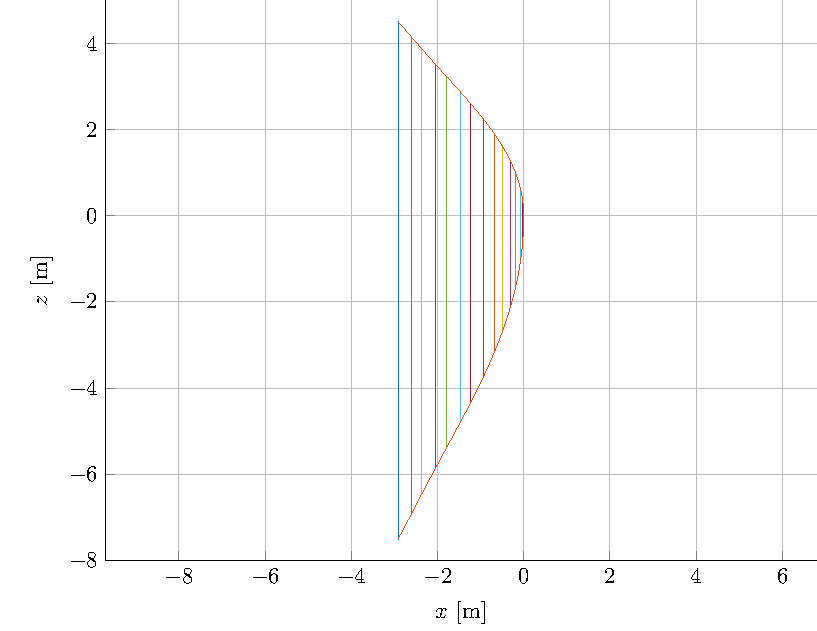
\includegraphics[width=1\textwidth]{./Figure/Aerodynamics/sideview_skewness.pdf}
		\captionsetup{width=0.9\textwidth,skip=-8pt}
		\caption[Side-view of a skewed aerodynamic shape]{Side-view of a skewed aerodynamic shape. The lower part generates a moment around the frontal part of the aeroshell when under an angle of attack}
		\label{fig:skewnessplot}
	\end{subfigure}
	\begin{subfigure}[t]{0.45\textwidth}
		\centering
		\captionsetup{width=0.9\textwidth}		
		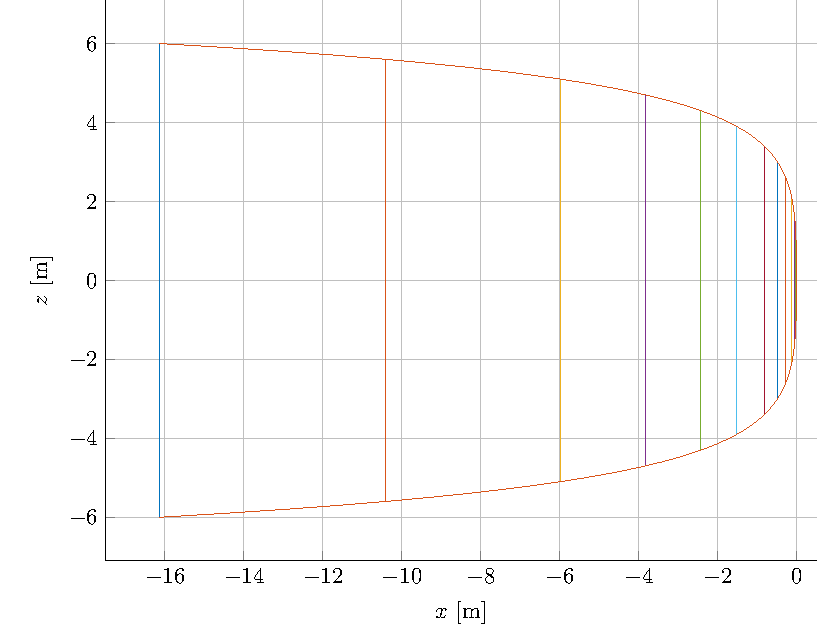
\includegraphics[width=1\textwidth]{./Figure/Aerodynamics/sideview_cmalpha.pdf}
		\caption{Optimised shape resulting in high static stability}
		\label{fig:highcmalphashape}
	\end{subfigure}	
	\caption{Skewed and statically stable aerodynamic shapes}
\end{figure}
	

\paragraph{Various shapes} \label{sec:aeroshapes}
Several large groups of varying shapes can be identified. The relative performance of each group can be qualitatively assessed by looking at the variations of the shape with respect to the optimal shapes for the various parameters. The effect of asymmetric cross-sections will be ignored in this assessment, and will be investigated separately. In Figure \ref{fig:aeroshapes} representative cross sections of the groups can be seen. Group A represents simple concave surfaces. Group B has a concave centre section with a flat ring around it. Group C has an approximately flat central section, with steep edges around the outer radius. Group D represents the half cone shapes, with relatively straight sides and a blunt nose. 

\begin{figure}[h]
	\centering
	
\includegraphics[width=0.5\textwidth]{./Figure/Aerodynamics/AeroShapes.pdf}
	\caption{Various schematic aerodynamic configurations}
	\label{fig:aeroshapes}
\end{figure}

As was discussed in this section, a flat plate will generate the most lift and the most drag, albeit at different angles of incidence. Since Group C closely mimics a flat plate in the majority of its cross-section, it will have the best lift and drag performance. Group B also has a significant flat section and will therefore also have good performance in terms of lift and drag. Groups A and D will both have significant portions of their cross-sections at sub-optimal incidence angles for maximum lift or drag, and will therefore have lower lift and drag performance.

The \gls{sym:cm-alpha} of a given shape is a measure of stability. Shapes which require large moments to change the angle of attack have a higher stability. As can be seen in Figure \ref{fig:CLCD-incidence}, surfaces at incidence angles of 40 to 60 $\left[deg\right]$ provide large changes in force for small changes in angle of incidence. Sections at these incidence angles will therefore stabilise the vehicle, since a change in angle of attack will cause one side of cross section to generate a greater moment than the other. This is visualised in Figure \ref{fig:StabMom}. Cross sections B and C have parts of their cross section at such angles. Since the sections in C are on the outside of the cross section, it will be significantly more stable than type B due to the moment arm these parts have. A and D will have significant portions of their cross sections contribute to the vehicle moment. Although these section are likely to be at sub optimal angles of incidence for high stability, the large area contributing to the stability of the vehicle will ensure that both types of cross section are stable. 


\begin{figure}[h]
	\centering
	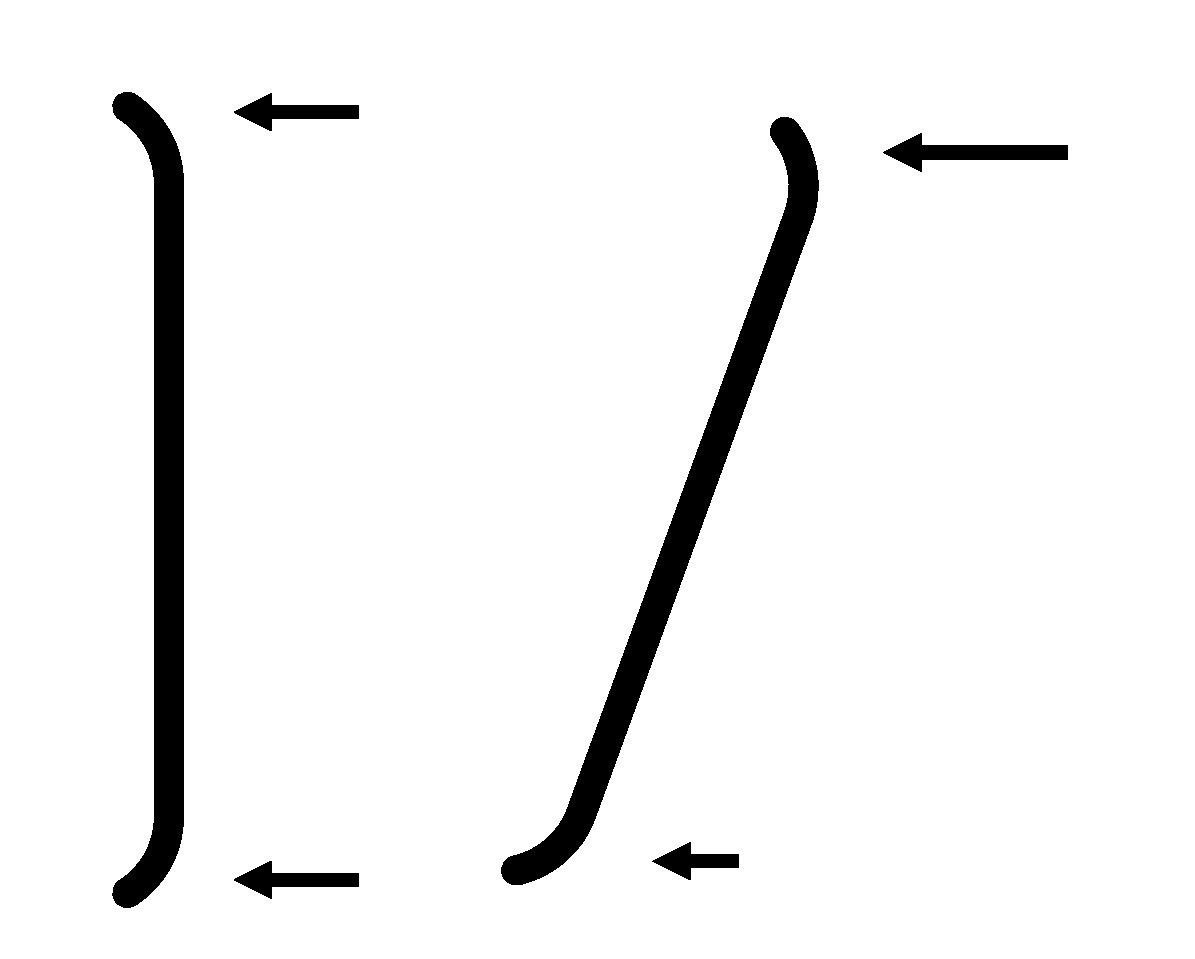
\includegraphics[width=0.5\textwidth]{./Figure/Aerodynamics/StabilizeMoment.pdf}
	\caption{Stabilising effect of reduced incidence angle sections}
	\label{fig:StabMom}
\end{figure}

\paragraph{Asymmetry}
An asymmetric body will ensure that even at zero degrees angle of attack, the vehicle generates lift. As explained in Section \ref{subsec:orbitsens}, this allows for greater control of the vehicle during aerocapture and entry and is therefore desirable. The angle of attack that can be attained is limited by the crew module extending into the flow around the body. Achieving a higher lift at a lower angle of attack is therefore desirable. If the shape is heavily offset to one edge of the body, the crew module will extend into the flow at very low angles of attack. Figure \ref{fig:LDSkew} shows the effect of asymmetry on the lift-to-drag ratio by transforming a given symmetric shape into an asymmetric shape. The asymmetric shapes are created by a linearly shifting the cross sections of the body in the $zy$-plane along the $y$-axis, with no shift at $x=0$ and maximum shift at $x=x_{max}$. 

\begin{figure}[h]
	%\centering
	\hspace{-8mm}
	\setlength\figureheight{0.4\textwidth} 
	\setlength\figurewidth{0.95\textwidth}
	\input{./Figure/Aerodynamics/LoverDplot.tikz}
	\caption{Effect of asymmetric shape on lift-to-drag ratio}
	\label{fig:LDSkew}
\end{figure}


\subsubsection{Control system analysis}\label{subsec:controltool}
\subsection{Control}

**Intro**

\subsubsection{Assumptions}

**Primary and Secondary assumptions**

\subsubsection{Trim point}

**Moment equilibrium figures/equations**
**CG-location plot(s)  with conclusion on CG for AoA~20 and sideslip angle=0**

\subsubsection{Stability}

**From E.Mooij**

\subsubsection{Available control systems}

**Intro**

\paragraph{\acrfull{cg} offset}

**Not nessesary for AoA, not feasible for sideslip**

\paragraph{Thrusters}

**Sebstiaan**

\paragraph{Aerodynamic surfaces}

**Guido**





\subsubsection{Thermal analysis}\label{subsec:thermaltool}
To investigate the influence of lay-up materials, heat flux variations, vehicle diameter and the trajectory approach on the \gls{tps} a sensitivity analysis is performed. First materials are selected to form multiple lay-ups. The different lay-ups are then optimised for different loading conditions. First the influence of heat flux variations on areal density is investigated. Subsequently, variations in mass due to changing diameters are tested. Lastly, the lay-ups are tested for different trajectories, either with a direct trajectory or with a parking orbit between aerocapture and landing. This investigation is done by using the tool described in Section \ref{subsec:thermaltool} and successfully validated in Appendix \ref{sec:VandVthermo}.

\paragraph{\gls{tps} materials}
Table \ref{tab:tpsmatprop} shows the materials that are used in the inflatable heat shield. A more extensive list of possible \gls{tps} materials and their properties can be found in Appendix \ref{sec:Thermoprop}. These materials have been proposed during the design of multiple inflatable decelerator concepts, such as \gls{irve} and \gls{thor} \cite{Hughes2005}. For each material the thermal conductivity, the density, the specific heat, the maximum operative temperature and if applicable, the emissivity are given. The latter is only applicable to the upper thermal protection layers, because these layers, or heat barriers, will radiate heat into the surroundings.
\newline\newline
A selection is made for the most promising thermal protection and insulation layers. These are Nextel BF-20 and Nicalon for the heat barrier layers. Nextel is a material already used by \gls{nasa} in \gls{irve}. Nicalon is a heavier alternative made up of continuous fibres of silicon carbide (SiC) that can withstand higher temperatures than Nextel up to $2073 \left[K\right]$. Also the emissivity of Nicalon is much higher that Nextel, which allows for more radiation. For the insulation layers these are Pyrogel\textsuperscript{\textregistered} 3350 and Pyrogel\textsuperscript{\textregistered} 6650. With those materials three lay-ups are created such that a comparison can be made between the heat barriers and insulators. A schematic view of the layers is shown in Figure \ref{fig:layersensthermal}. Lay-ups 1 and 2 can be used to compare the performance of Pyrogel\textsuperscript{\textregistered} 3350 and 6650. Lay-ups 2 and 3 serve as comparison for the Nextel BF-20 and Nicalon. These lay-ups will be tested for different heat fluxes as well as different diameters.

\begin{table}[ht]
	\caption {Flexible \acrlong{tps} material properties \cite{Corso2009,Corso2011,DuPont2011,Smith2011,Nye,Zinkle1998}}
	\centering
	\begin{tabular}{|l|l|l|l|l|l|l|}
		\hline
	        \textbf{Material}         & \textbf{ $\mathbf{k}$ $\mathbf{\left[\frac{W}{m\cdot K}\right]} $} & \textbf{ $\mathbf{ \rho }$ $\mathbf{ \left[ \frac{kg}{m^3} \right] }$} & \textbf{  $\mathbf{ c_{p} }$ $\mathbf{ \left[ \frac{J}{kg \cdot K} \right] }$ }& \textbf{ $\mathbf{ T_{max} }$ $\mathbf{ [ K ] }$} &\textbf{ $\mathbf{ \varepsilon }$ $\mathbf{ [ - ] }$} & \textbf{Function} \\[1.6ex]   \hline \hline
		Hi-Nicalon			& 2.4			& 2900	& 1200	& 2073	& 0.93	& rad. \& barrier	\\ \hline
		Nextel BF20			& 0.146			& 1362	& 1130	& 1643	& 0.443	& rad. \& barrier	\\ \hline
		Pyrogel\textsuperscript{\textregistered} 6650		& 0.030			& 110	& 1046	& 923	& -		& insulator			\\ \hline
		Pyrogel\textsuperscript{\textregistered} 3350		& 0.0248		& 170	& 1046	& 1373	& -		& insulator			\\ \hline
		Kapton				& 0.12			& 1468	& 1022	& 673	& -		& gas barrier		\\ \hline
		Kevlar				& 0.04			& 1440	& 1420	& 443	& -		& structural		\\ \hline
		PBO Zylon\textsuperscript{\textregistered}			& 20			& 1540	& 900	& 673	& -		& structural		\\ \hline

	\end{tabular}
	\label{tab:tpsmatprop}
\vspace{-4mm}
\end{table}

\begin{figure}[h]
	\centering
	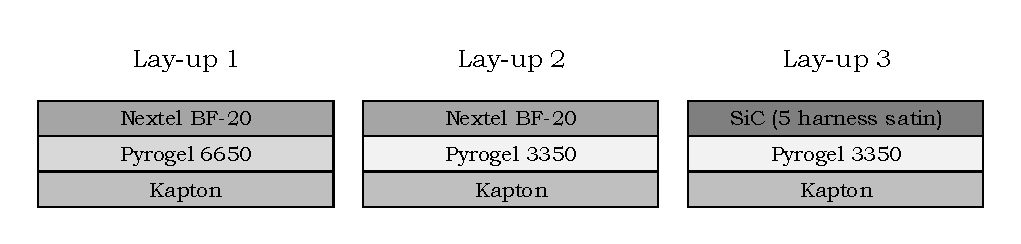
\includegraphics[width=\textwidth]{./Figure/Thermal/layersensthermal.pdf}
	\caption{Tested lay-ups for the sensitivity analysis}
	\label{fig:layersensthermal}
\end{figure}

\paragraph{Effect of heat flux}
In order to analyse areal density performance of lay-ups and changes due to varying atmospheric conditions a heat flux sensitivity is performed. To achieve this, ratios of the heat flux of a possible trajectory are used. The trajectory is found using a diameter of $12 \left[ m \right]$. The results are shown in Figure \ref{fig:sensitivityq}. The horizontal axis shows the heat flux ratio and the areal density is shown on the vertical axis. 

\begin{figure}[h]
	\centering
	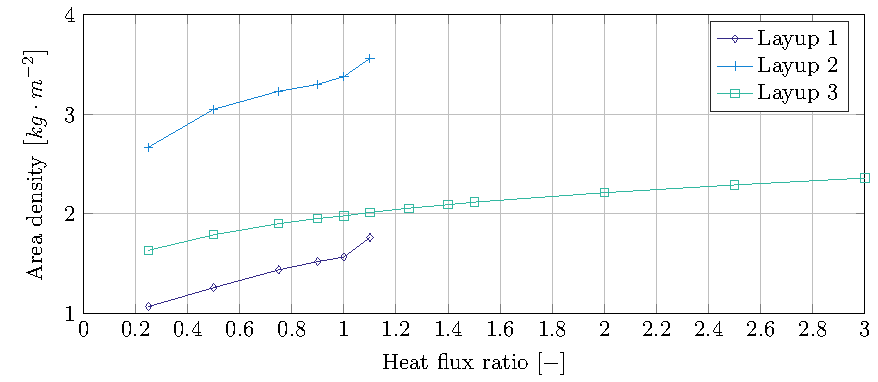
\includegraphics{./Figure/Thermal/Sensitivityq.pdf}
	\caption{Heat flux sensitivity for the three selected lay-ups}
	\label{fig:sensitivityq}
\end{figure}


As expected, the mass of the \gls{tps} increases with increased loading. Secondly and most important, the relative performance of the lay-ups can be observed. Lay-up 1 is clearly the lightest solution, followed by lay-up 3 and 2. Although lay-up 1 performs better in terms of its mass, the amount of loading it can bear is limited. If small changes in atmospheric properties occur during the \gls{edl} phase, for instance due to Martian storms, the \gls{tps} may succumb under the increasing loads. Therefore it is wise to choose Nicalon for further design. Lastly, if lay-up 1 and 3 are analysed relative to each other, it is clear that Pyrogel\textsuperscript{\textregistered} 6650 performs much better than the 3350 variant. Therefore, for further design it is more favourable to use Pyrogel\textsuperscript{\textregistered} 6650 as an insulator. The drawback of Pyrogel\textsuperscript{\textregistered} 6650 is that it has a lower maximum use temperature. This is solved by using a good heat barrier such as Nicalon.

\paragraph{Effect of diameter}
The three lay-ups are put to the test for different diameters. Aerodynamic analysis has provided heat fluxes for trajectories with corresponding diameters of $6$, $9$, $12$, $15$ and $18 \left[ m \right]$. As a side note, because the aerodynamic shape is different from the one in the previous paragraph, Figures \ref{fig:sensitivityq} and \ref{fig:sensitivityA} cannot be directly compared. An increase in heat flux caused an increase in the maximum temperature, surpassing the Nextel operative temperature limit which made it impossible for lay-ups 1 and 3 to fly trajectories at diameters of $12 \left[ m \right]$. Optimising the thickness of the lay-ups for these heat flux result in Figure \ref{fig:sensitivityA}. The solid lines indicate the nominal trajectory, with a parking orbit after aerocapture. For both graphs, the horizontal axis shows the relevant diameters. The plot on the left shows the areal density on the vertical axis and the right plot shows the total mass of the frontal \gls{tps} on this axis.

\begin{figure}[h]
	\centering
	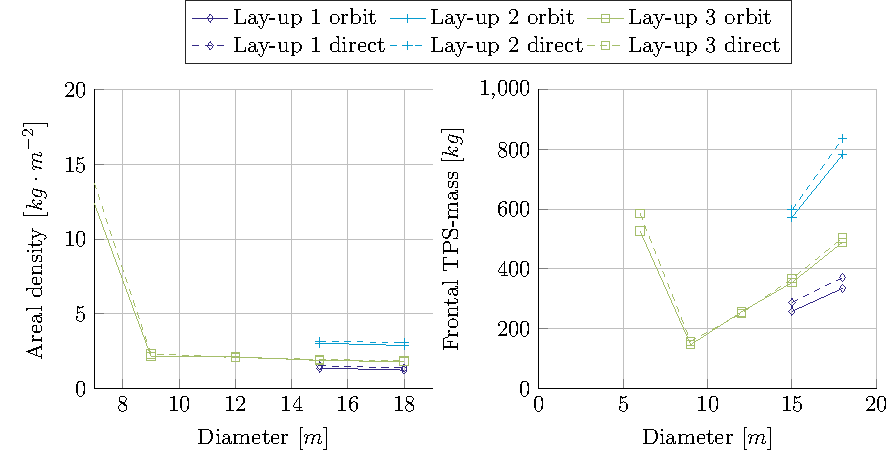
\includegraphics{./Figure/Thermal/SensitivityA.pdf}
	\caption[Areal sensitivity for the three selected lay-ups]{Areal sensitivity for the three selected lay-ups, both for a direct trajectory and a usual trajectory with a parking orbit after aerocapture. Left plot shows areal density, whereas the right plot shows the total mass.}
	\label{fig:sensitivityA}
\end{figure}

For increasing diameters, larger radii of curvature can be obtained, resulting in a direct decrease of incoming heat flux. Also, due to the increasing diameters which causes an increase in \gls{sym:CD} and a reduction in ballistic coefficient, the vehicle can decelerate by the same amount at lower dynamic pressures. Therefore, the vehicle can stay higher in the atmosphere and fly in thinner air with the same velocity, decreasing heat development and incoming heat flux.\\

This effect can clearly be seen in the left figure, where the areal density decreases for increasing diameters. Obviously more material must be used to create larger \gls{tps}, which mostly results in a total mass increase for larger diameters. This can be seen in the right figure. The only exception is lay-up 2, the lay-up that is able to cope with the larger incoming heat flux at lower diameters. An optimum of its thermal performance is found at $9 \left[ m \right]$ where the frontal \gls{tps} mass reduces to approximately $150 \left[ kg \right]$. In addition, the relative mass performance of the different lay-ups is comparable to the performance in the previous paragraph.

\paragraph{Effect of time}
Whenever the vehicle is changing its descend rate, the total dissipated energy is still the same. However, the energy rate profile will have a different distribution over time, changing the temperature throughout the \gls{tps}. Steeper descends require a thicker heat barrier, limiting the heat flow to the rest of the shell, such that operational temperature of the insulator is not exceeded. A more gradual descend increases the time spend in the atmosphere and therefore increases the heat stored in the heat shield. This puts limits on the insulators minimum thickness, to block the heat flow to the structural layers and the rest of the vehicle. Therefore, the effect of descent time is analysed. The results are also shown in Figure \ref{fig:sensitivityA}. An alteration in time is visible by considering two types of viable trajectories, a direct trajectory and one with an orbit after aerocapture. From the figure it can be seen that the direct trajectory is the limiting one.

\subsubsection{Structural analysis}\label{subsec:structool}
\paragraph{Inflatable structural mass}

Based on the mass estimation model outlined in subsection \ref{subsec:structool}, the effect of changing design parameters on inflatable structural mass is investigated hereafter. To this end, the following design parameters have been investigated: centerbody and inflated diameter, half-cone angle, the number of toroids and aerodynamic loading. The drag coefficient has not been investigated separately, for it appears exclusively multiplied by dynamic pressure and a percentual increase in drag coefficient therefore has the same effect as an equal percentual change in dynamic pressure. The product of these two terms gives the aerodynamic force working over the decelerator frontal surface area.

\begin{figure}[ht]
	\centering

	\begin{subfigure}[b]{0.49\textwidth}
		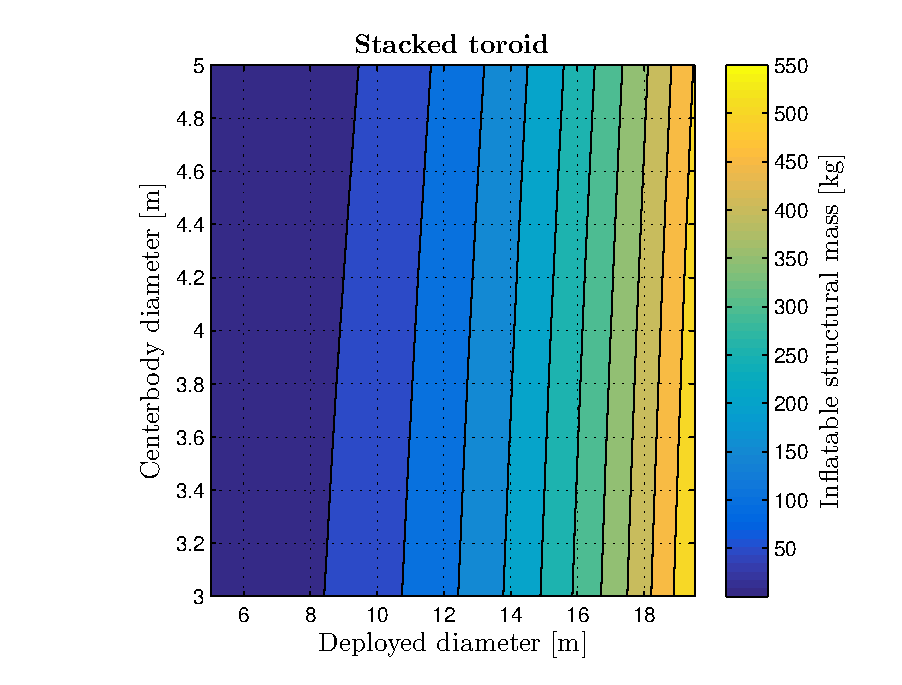
\includegraphics[width=0.96\textwidth]{./Figure/Structure/diameters_test.eps}
		\caption{Mass versus centerbody and deployed diameter}
		\label{fig:diameters_strucmass}
	\end{subfigure}
	\begin{subfigure}[b]{0.49\textwidth}
		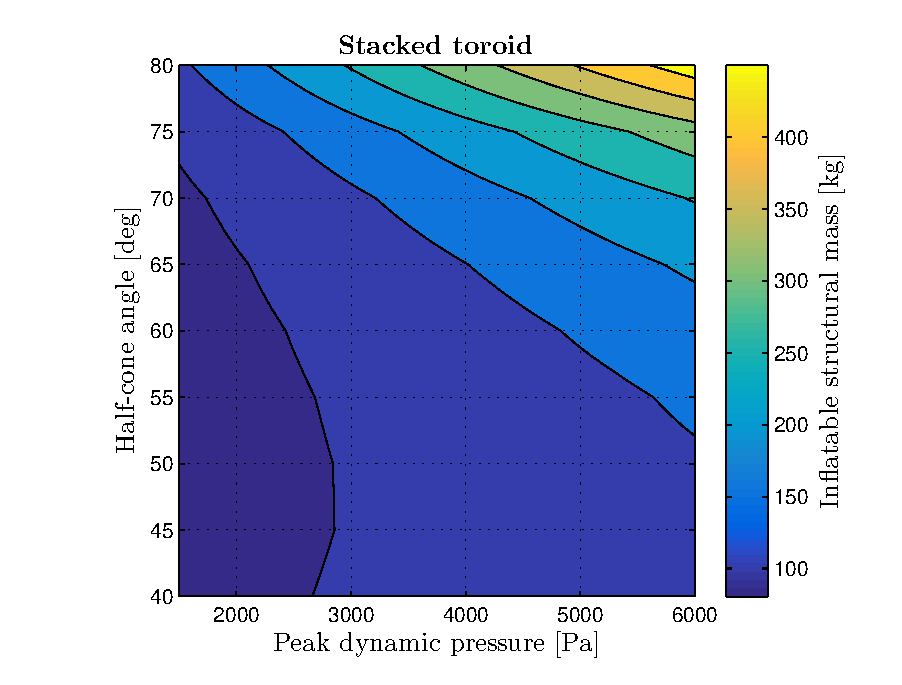
\includegraphics[width=0.96\textwidth]{./Figure/Structure/halfcone_test.eps}
		\caption{Mass versus half-cone angle and peak dynamic pressure}
		\label{fig:halfcone_strucmass}
	\end{subfigure}
	\begin{subfigure}[b]{0.49\textwidth}
		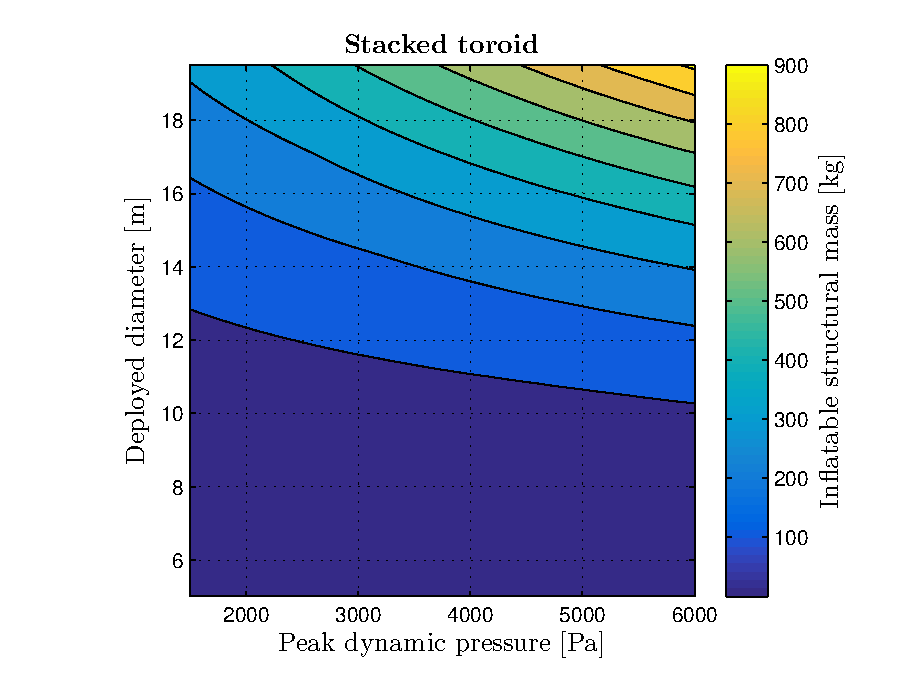
\includegraphics[width=0.96\textwidth]{./Figure/Structure/pressure_test.eps}
		\caption{Mass versus deployed diameter and peak dynamic pressure}
		\label{fig:press_strucmass}
	\end{subfigure}
	\begin{subfigure}[b]{0.49\textwidth}
		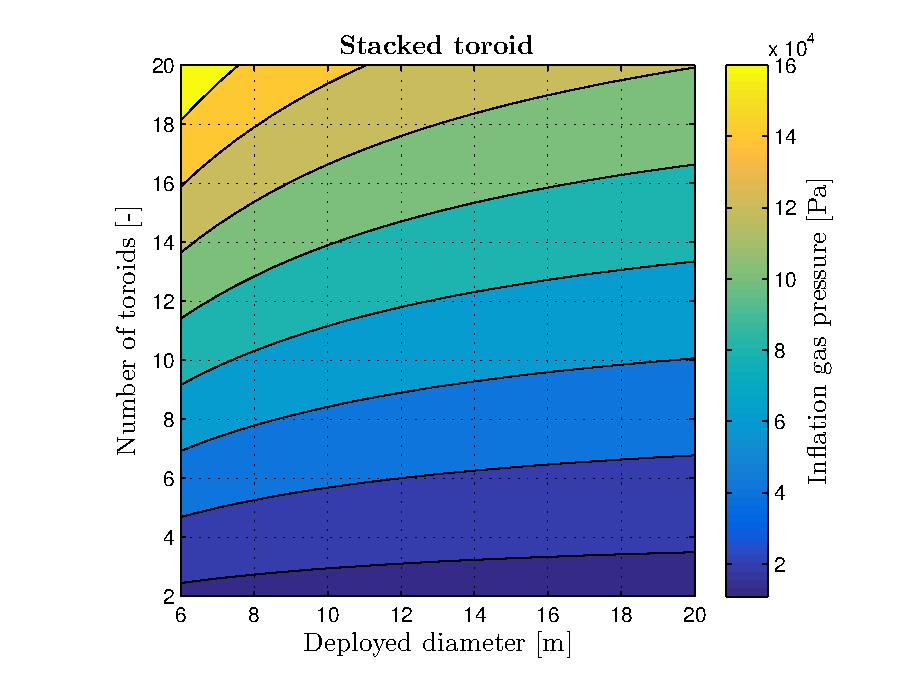
\includegraphics[width=0.96\textwidth]{./Figure/Structure/inflation_test.eps}
		\caption{Inflation pressure versus number of toroids and deployed diameter}
		\label{fig:inflpress_strucmass}
	\end{subfigure}
\caption{Inflatable structural mass and inflation pressure as a function of design parameters}
\end{figure}
Firstly, from Figure \ref{fig:diameters_strucmass} it follows that mass decreases with an increasing centerbody diameter given a deployed diameter. This is due to the fact that an increasing centerbody diameter increases the areal contribution of the centerbody: the inflatable requires less structural mass by decreased aerodynamic loading thereof, as aerodynamic pressure works over an area. In turn, this suggests that the centerbody becomes heavier, which is not the case as the centerbody is typically sized for launch rather than (re-)entry loads \cite{Lindell2006}. It can therefore be concluded that maximizing centerbody diameter is beneficial for structural mass. 

Secondly, from Figure \ref{fig:press_strucmass} it follows that increasing dynamic pressure effects an increase in structural mass of the inflatable. This is the result of an increased aerodynamic loading and therefore structural taxation of the inflatable. To withstand this loading, extra structural mass is required. Moreover, for a given peak dynamic pressure an increase in deployed diameter effects an increase in structural mass. Primary cause hereof is the fact that pressure works over a surface area and an increase in area thereby increases the loading. This is further amplified by an increase in bending moments by the larger distance from tip to root.

From Figure \ref{fig:halfcone_strucmass} it may be observed that the half-cone angle significantly affects inflatable structural mass: in general smaller half-cone angles are preferable. Increasing half-cone angle beyond an optimum region at approximately 45 degrees strongly increases structural mass; decreasing it below this region similarly increases structural mass, but less strongly. Moreover, as aerodynamic loading is increased the optimum region shifts and smaller half-cone angles are preferable. This is due to the fact that decreasing the half-cone angle increases bending stiffness by an increased moment of inertia in the bending plane. This increased bending stiffness is further amplified by the three-dimensionality of the sphere cone and carries over to more effective use of material in bending, requiring less mass to resist the bending moment by aerodynamic loading. For a given deployed diameter, however, decreasing the half-cone angle increases the effective inflatable length. This addition of material is to be traded off against the increased bending material. At low dynamic pressures, increased bending stiffness is less warranted than at higher pressures, at which bending loads increase and bending stiffness is increasingly more warranted.

In Figure \ref{fig:inflpress_strucmass} inflation gas pressure is observed to increase for an increasing number of toroids and to decrease with an increasing deployed diameter. Both an increase in the number of toroids and a decrease in deployed diameter decrease toroid radii, effecting an increase in the working area of the inflation pressure. Due to the proportionality of the running load induced by inflation pressure via Equation \ref{eq:Pmin} with toroid radius, a larger inflation pressure is required to induce the same running load with a smaller radius. This running load is based on the consideration that the work done by inflation gas and external forces in axial direction are equal \cite{Brown2009}, independent of the number of toroids. It is similarly independent of the deployed diameter, since both inflation and aerodynamic pressure have the same working area in axial direction.
%The thickness required increases with decreasing material ultimate strength, which explains the differences in structural mass observed between different materials at low dynamic pressures. These differences carry through as loading is increased, where materials with a higher specific strength require less mass to withstand the loading. The material used in \gls{irve}-3, PBO Zylon, is observed to offer notable mass advantages over heritage aramid fibers, such as Kevlar. Mass reduction beyond this level is possible by using Technora and Spectra 2000. All materials are selected based on their operating temperature since these are required to operate in an environment with significant thermal loading. A summary of material properties is given in the Mid-Term Report \cite{Balasooriyan2015b}.
The number of toroids was observed to have no significant effect on structural mass beyond ten toroids, after which mass reductions were found to be within two percent. An increase in the number of toroids from two to ten yields significant mass advantages of up to ten percent. 



Material selection has a significant effect on flexible material mass, as illustrated by Figure \ref{fig:mat}. It can be observed that, for peak dynamic pressures below 2 [$kPa$], minimum gage thickness is leading for all selected fibres. Below this pressure, density is the leading parameter and a less dense material will perform better. Due to the significantly lower density of Spectra 2000, 970 [$kg \cdot m^{-3}$], versus that of for example PBO Zylon, 1540 [$kg \cdot m^{-3}$], Spectra 2000 offers mass advantages at low dynamic pressures. Therefore it can be concluded that for low dynamic pressures materials should be selected based on minimum gage thickness, but thickness rapidly increases as loading is increased and the minimum gage thickness is exceeded. For PBO Zylon, this occurs at a relatively high peak dynamic pressure of 3.5 [$kPa$].

For higher dynamic pressures, materials with a higher specific strength perform better in terms of structural mass. Flexible material is fully loaded in tension by the inflation pressure is required not to fail under tension, dictated by ultimate strength. To this end, a certain thickness with a corresponding mass is required. Mass performance is then directly linked to specific strength and this is confirmed by Figure \ref{fig:mat}. Aramid fibres Kevlar and Technora have the lowest specific strengths, approximately 2 [$MNm \cdot kg^{-1}$]. A notably higher specific strength of 3.44 and 3.77 [$MNm \cdot kg^{-1}$] is attained by Spectra 2000 and PBO Zylon respectively. This confirms the choice for PBO Zylon for its mass advantages over Kevlar in \gls{irve}-3 \cite{Dillman2012a}. Spectra 2000 is capable of achieving a lower mass than PBO Zylon despite its lower specific strength, due to its low density. 

Mass differences between materials remain limited, up to 30 [$kg$] over a range of half-cone angles and diameters.

All materials have been selected based on their operating temperature since these are required to operate in an environment with significant thermal loading. As an example, Spectra 2000 fibres are not deemed suitable for their allowable temperature of 150 degrees Celsius, which would incur significant extra \acrfull{tps} mass. Dyneema would similarly be unsuitable by its temperature limit of 145 degrees Celsius\footnote{URL:\url{http://eurofibers.com/fibers/dyneema/}. Accessed: 17-06-2015} A summary of material properties is given in the Mid-Term Report \cite[p.64]{Balasooriyan2015b}. 

\begin{figure}[ht]
	\centering
	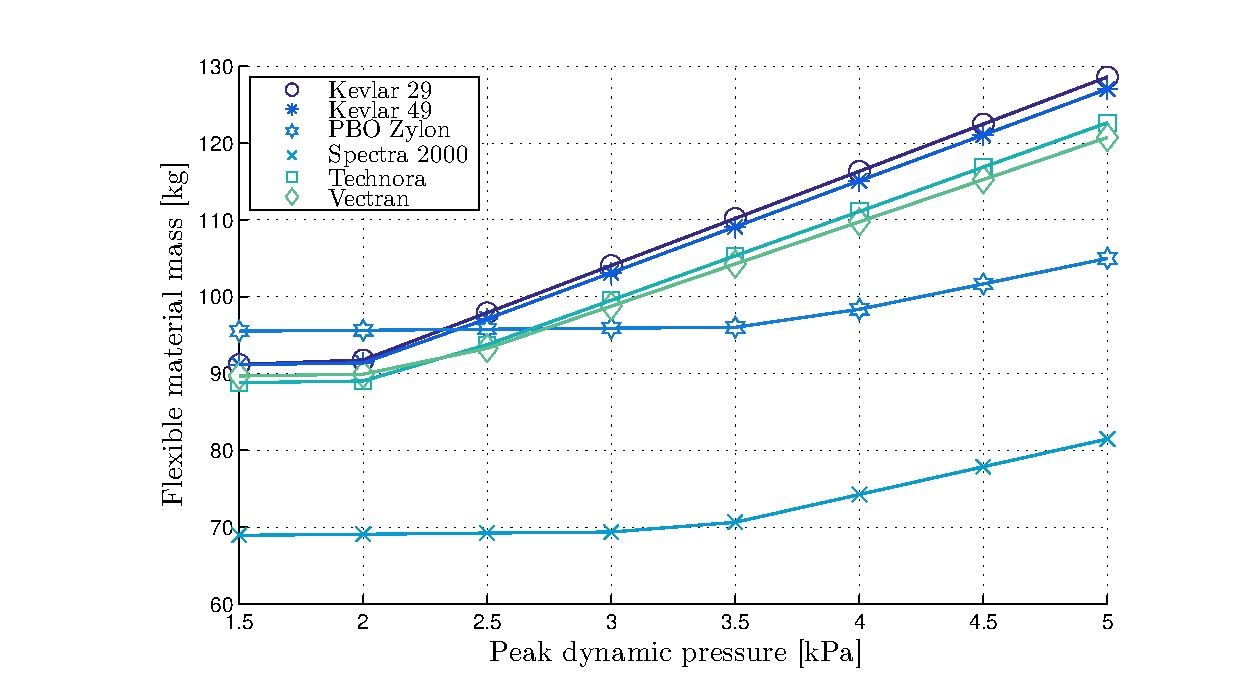
\includegraphics[width=1.0\textwidth]{./Figure/Structure/material_test2.eps}
	\caption{Flexible material structural mass estimation for different materials}
	\label{fig:mat}
\end{figure}

\paragraph{Forces}

Using the force estimation tool for the inflatable structure the sensitivity for the scaling of loads can be determined. Figure \ref{fig:forces} displays the estimated structural loads throughout the inflatable for a total of 9 toroids and a set outer diameter of 12 and 18 [$m$]. The loads as displayed in Figure \ref{fig:forces} feature solely the loads induced by aerodynamic pressure. The internal pressure loads follow separately. This sensitivity analysis is performed to evaluate the scalability of the \gls{hiad} design. Previous \gls{hiad} designs, most predominantly the \gls{irve} missions, feature smaller mission payloads and corresponding smaller diameters. Up to this point the highest diameter stacked toroid design flown is featured in the second and third \gls{irve} missions, namely an outer diameter of 2.93 [$m$]. 

\begin{figure}[ht]
	\centering
	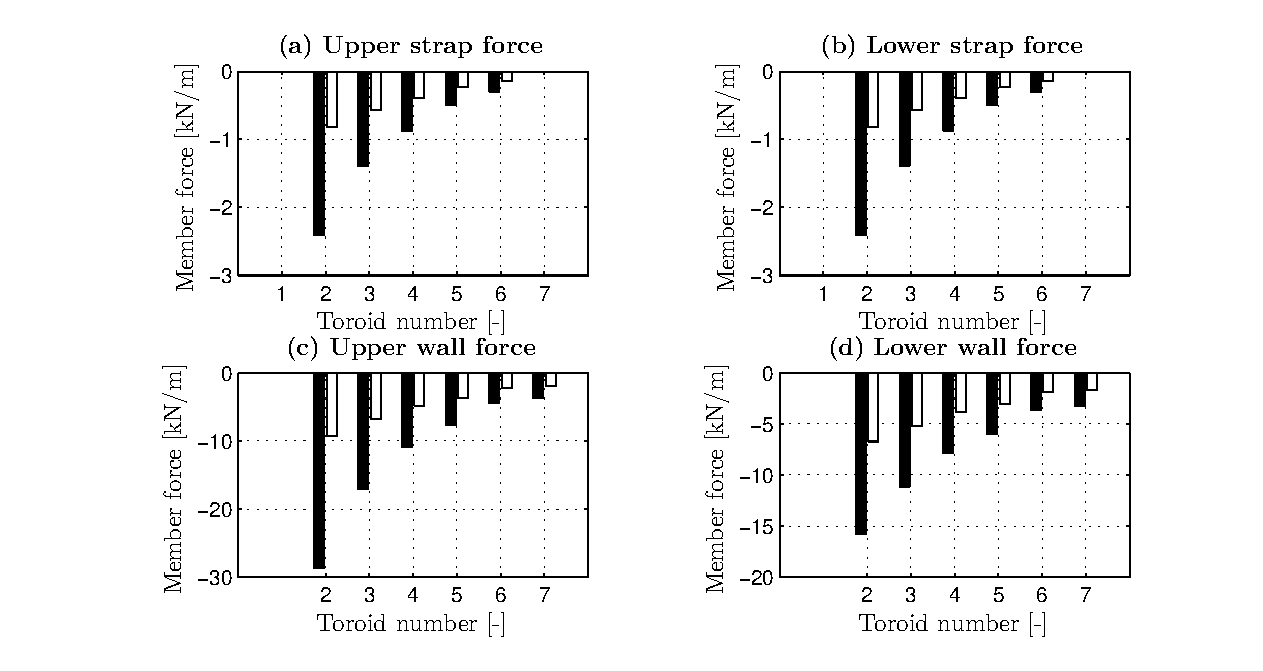
\includegraphics[width=0.9\textwidth]{./Figure/Structure/forces_nopress_test.eps}
	\caption[{Internal force estimation for dynamic pressure 3750 [$Pa$], no inflation pressure applied}]{Internal force estimation for dynamic pressure 3750 [$Pa$], no inflation pressure applied. Black bars are for a diameter of 18 [$m$]; white bars for a diameter of 12 [$m$]}
	\label{fig:forces}
\end{figure}

\begin{figure}[ht]
	\centering
	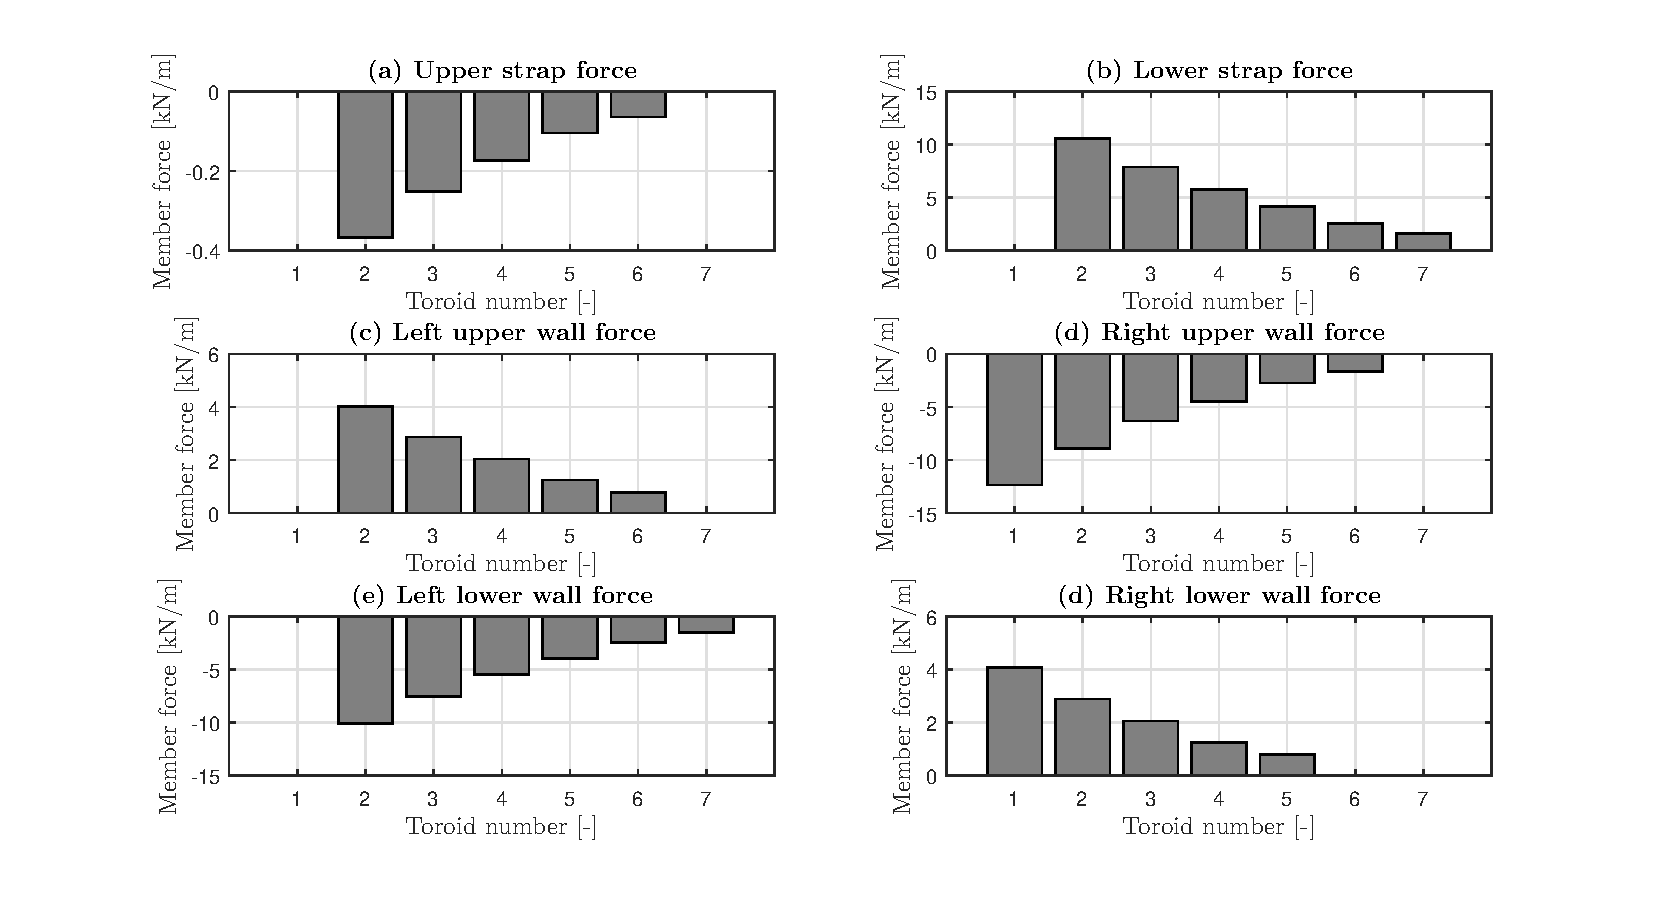
\includegraphics[width=0.9\textwidth]{./Figure/Structure/forces_test.eps}
	\caption[{Internal force estimation for dynamic pressure 3750 [$Pa$], with inflation pressure applied}]{Internal force estimation for dynamic pressure 3750 [$Pa$], with inflation pressure applied. Black bars are for a diameter of 18 [$m$]; white bars for a diameter of 12 [$m$]}
	\label{fig:forcesp}
\end{figure}

From the results of Figure \ref{fig:forces} several conclusions can be made. Most importantly it shows that scaling of the inflatable is possible. Although a load increase can be observed for increasing diameter, this follows only from the additional axial loads. The induced bending moment is not represented in Figure \ref{fig:forces} as this is carried circumferentially. This followed from the verification and validation procedures explained in more detail in Appendix \ref{sec:VandVstruc}. Moreover, loads are found to be within material capabilities.

Secondly the loads do not increase linearly over the diameter. This is the result of the scaling of the loads, to account for the decreasing circumference over which forces act. The reducing diameter causes an additional increase of the loads per unit length.

Thirdly the dynamic pressure loads of Figure \ref{fig:forces} are found to be of a similar order as the internal pressure loads induced per Equation \ref{eq:Q} at the root of the inflatable. Moving towards the tip of the inflatable these differences increase as the internal pressure loads are maintained whereas the loads induce by the dynamic pressure reduce towards the tip. This is further expanded upon in Figure \ref{fig:forcesp} in which pressure loads are included.

The final conclusion with regards to scalability of the inflatable can be made on the basis of Figure \ref{fig:forcesp}. If the internal and external pressure loads are combined a minimum required thickness can be computed on the basis of requiring the structure not to yield. This parameter is relevant as foldability of the inflatable has to be considered as well. Foldability is an important parameter as the inflatable has to be stowed away during launch and the transfer towards Mars. From this yielding criterion and a typical material such as Kevlar 49 a minimum required thickness of below 0.01 [$mm$] is found. Since this value is rather small the thickness of the inflatable is not a consideration from a folding perspective even for large diameters.







\subsection{Design parameter sensitivity} \label{sec:designsens}
The following sections present an overview of design characteristics as obtained by the analysis and design tools presented in this chapter. Sensitivity analysis is limited to those parameters of key importance for the mission.
\subsubsection{Trajectory sensitivity}\label{subsec:orbitsens}
\paragraph{Input and output}
As input the tool requires the entry velocity, flight path angle at the boundary of the atmosphere, an aerodynamic model (\gls{sym:CL} and \gls{sym:CD} as a function of \gls{sym:alpha}), an \gls{sym:alpha}-profile (changes in the angle of attack during the aerocapture and entry), and a \gls{sym:mu} profile (changes in the bank angle during the aerocapture and entry).

As output the trajectory tool can generate important parameters at each moment in time. The most important parameters are: location (\gls{sym:Rv}), acceleration $\left(\gls{sym:acc}\right)$, dynamic pressure $\left(\gls{sym:q}_{\infty}\right)$, velocity $\left(\gls{sym:Vv}\right)$, Mach number $\left(\gls{sym:M}\right)$, atmospheric temperature $\left(\gls{sym:T}_{\infty}\right)$ and atmospheric density $\left(\gls{sym:rho}_{\infty}\right)$.

\paragraph{Assumptions}
 \label{sec:astroassumption}
 Some of the assumptions have a big impact, these are the primary assumptions. There are, however, also some assumptions that have a negligible effect on the results. These are the secondary assumptions.
 
 \subparagraph{Primary assumptions}
 \begin{itemize}
 \item All atmospheric properties only vary with the height above \gls{mola} and not with longitude, latitude or time. These variations are shown in Appendix \ref{app:atmos}. 
 \item All trajectories are assumed to only occur in the equatorial plane. This means that the latitude is always $0 \left[deg\right]$. Changing the latitude will have a big impact on the relative speed of the Martian atmosphere.
 \item The gravitational pull is assumed to only vary with the height above \gls{mola}. The gravitational field of Mars is however not uniform over longitude and latitude, this will induce errors in the trajectory as gravity is one of the major forces in the analysis.
 \item The bank reversals needed for bank control are assumed to be instantaneous.
 \end{itemize}

 \subparagraph{Secondary assumptions}
 \begin{itemize}
 \item The spacecraft is assumed to only feel a gravitational pull from Mars. It is thus assumed that there is no gravitational pull from the sun, any other planet or the Martian moons.
 \item The atmosphere stops at an altitude of 400 $\left[km\right]$. At this point the atmosphere is negligibly thin, expanding the atmospheric model would not contribute to the results.
 \item The effect of other disturbances i.e. solar radiation is neglected.
 \end{itemize}

\paragraph{Analysis method}
The orbit can be divided into two different parts, one part is the pass through the atmosphere and the other is outside of the atmosphere. In the first part, there are three forces working on the spacecraft: Lift, drag and gravity. In the second part there is only the gravitational force.

The part outside the atmosphere is simplified by using the Kepler equations of orbital motion to determine the position of the spacecraft over time.

The atmospheric properties are determined using the NASA software \gls{marsgram}. The software generates data based on equations for atmosphere properties and incorporates the high amount of dust on Mars, which has a big effect on the absorbed radiation heat from the sun. From this model the average atmospheric properties are used to determine the aerodynamic forces. All data used from \gls{marsgram} is shown in Appendix \ref{app:atmos}. 

Using the aerodynamic forces combined with the gravitational pull from Mars the accelerations are calculated. These accelerations are integrated twice to obtain the velocity and the location.

\paragraph{Limitations}
The tool is mainly limited by the 1D implementation of the atmospheric properties and gravity model. This means that no variations of the atmosphere over longitude, latitude or time are considered. It is recommended to implement the full atmospheric model in later stages of the design. The use of a numerical simulation only introduces a small error. The full verification and validation are done in Appendix \ref{sec:VandVtraj}.

\subsubsection{Aerodynamic sensitivity}\label{subsec:aerosens}



\paragraph{Important parameters}\label{sec:aeroparams}
 The following parameters were determined to have a significant influence on te performance of the vehicle:

\begin{itemize}
	\item{Lift. As detailed in Section \ref{subsec:orbitsens}, the vehicle requires a lift vector to provide flight path control. A larger lift vector provides an increase in flight path control.}
	\item{Drag. The vehicle decelerates purely on atmospheric drag. An increase in drag will decrease the required time for aerocapture and entry and provides greater flexibility in terms of the path through the atmosphere.}
	\item{Lift-to-drag ratio. The lift-to-drag ratio is an indication of the freedom in the selection of the orbital trajectory. A higher lift-to-drag ratio will provide greater flexibility.}
	\item{\gls{sym:cm-alpha}. The derivative with respect to angle of attack of the moment coefficient is a measure of the stability of the vehicle. }
	\item{\gls{cg} offset}. The \gls{cg} offset at a given angle of attack required to cancel the moment generated by the vehicle at that angle of attack. It is a measure of the control effort required to trim the vehicle. 
	\item{Heat flux. For a given flight condition, the heat flux in the stagnation point depends only on the vehicle geometry.  }
\end{itemize}


\paragraph{Shape sensitivity} \label{sec:aerooptima}
Obtaining favourable characteristics of the aerodynamic shapes requires understanding of the influence of shape parameters on the performance of the design. To this end, firstly an analytical approach is taken. After that, conclusions can be made about different aerodynamic shapes. The optimisation tool is used afterwards to generate shapes that are optimised for certain design parameters, such that the conclusions based on the analytical knowledge can be verified.

In Figure \ref{fig:CLCD-incidence}, the lift and drag performance as well as the lift-to-drag ratio of a flat plate in a free stream is given. Since Newtonian flow theory is based on the assumption that pressure only depends on the local body incidence angle, this plot can be used to deduce performance of a given shape. As can be seen in the plot, a vehicle with a high drag has most of its surface perpendicular of the flow.

\paragraph{Lift}
A high lift is achieved by having large parts of the shape under an incidence angle of 35 $\left[deg\right]$. An axisymmetric shape does not create lift at zero angle of attack, since every radial part of the shape cancels all non-drag forces out. Skewness of the shape, such as portrayed in Figure \ref{fig:skewnessplot}, can be used to create lift at zero angle of attack: a larger part of the surface is inclined upwards than downwards, meaning the skewed shape generates a downward lift. Using skewness instead of an axisymmetric body at a high angle of attack may help to prevent the shock wave from hitting the payload module.

\paragraph{Drag}
Maximum drag is created by having large parts of the shape perpendicular to the flow. This follows directly from Figure \ref{fig:CLCD-incidence}, in which it can be observed that maximum drag is generated at an incidence angle of 0 $\left[deg\right]$

\paragraph{Lift-to-drag ratio}
A high lift-to-drag ratio is achieved by having the highest angle of attack for every part of the spacecraft. This entails having a flat plate at the maximum angle of attack for maximum lift-to-drag ratio. If a non-flat body is chosen, large parts of the area should be nearly under a high inclination, which can be realised by having a very long body at a small angle of attack.

\paragraph{Static stability}
The aerodynamic shape required for static stability can be argued based on the local inclination angle. The pressure force always acts normal to the surface. A large moment arm can be created by inclining the outer edges of the aeroshell. At a positive angle of attack, the lower edge of the aeroshell is turned more perpendicular to the flow such that its pressure force is increased. An example of a shape that features this is given in Figure \ref{fig:skewnessplot}. Depending on the location of the \acrfull{cg}, at an angle of attack the lower part pressure is increased while the pressure on the upper part is decreased, generating a moment. This means that for an increase in angle of attack, the restoring moment is also increased.

\paragraph{Centre of Gravity shift}
In order to trim the aeroshell at a certain angle of attack, a \gls{cg} offset is used: the \gls{cg} does not lie directly on the most forward point of the spacecraft. In order to minimise the impact, the required \gls{cg} offset is calculated using Equation \ref{eq:reqcgoffset}. A large offset may be unrealistic and more difficult to implement.

\begin{equation} \label{eq:reqcgoffset}
z_{\gls{cg}} = \frac{\gls{sym:CM}\gls{sym:lref}}{\gls{sym:CL}}
\end{equation}
In general the relation between required \gls{cg} offset for a certain lift-to-drag ratio is a good indicator for the performance of a design, since this relates the performance to the cost of the performance.

Finally, the heat flux is given in Equation \ref{eq:modnewtonianqw} and is directly dependent on the density and velocity as well as the local radius of curvature. A less curved body in the stagnation point thus leads to a lower heat flux.

\begin{figure}[h]
	\centering
	\setlength\figureheight{0.4\textwidth} 
	\setlength\figurewidth{0.95\textwidth}
	\input{Figure/Aerodynamics/LDplot.tikz}
	\caption{Lift, drag and lift-to-drag ratio for a flat plate versus incidence angle}
	\label{fig:CLCD-incidence}
\end{figure}

To illustrate the characteristics of different aerodynamic shapes, an optimisation has been performed towards certain aerodynamic coefficients, as explained in Section \ref{par:Optimisation}. These shapes serve to enlarge understanding of how certain shape aspects correspond to certain aerodynamic properties. For the following parameters has been optimised:
\begin{itemize}
	\item Drag coefficient \gls{sym:CD}: The maximum drag should be attained by a flat plate at a zero angle of attack. This is also the result of the optimisation towards a maximal drag.
	\item Lift coefficient \gls{sym:CL}: As per the analysis in this Section, the maximum lift coefficient is achieved by a flat plate at an angle of attack of 35 $\left[deg\right]$. This is confirmed by the optimisation algorithm, which produces the same flat plate as for maximum drag, but at an angle of attack.
	\item Lift over Drag $\frac{\gls{sym:L}}{\gls{sym:D}}$: The maximum lift-to-drag ratio is found for a flat plate at an angle of attack as high as possible. This result was achieved at an angle of attack of 40 $\left[deg\right]$, which is limited to keep the design in the range where the shockwaves do not hit the payload module.
	\item Static stability \gls{sym:cm-alpha}: For this parameter, it is necessary to have large parts of the aerodynamic shape inclined with respect to the flow. The optimisation confirms this and creates a shape as portrayed in Figure \ref{fig:highcmalphashape}. This optimisation was constrained by a maximum length.
	\item \gls{cg} shift $\frac{\gls{sym:CM}}{\gls{sym:CX}}$: The minimum \gls{cg} shift for a given angle of attack is achieved by a flat plate since it generates very little moment. However, if static stability is required, the contours of the aeroshell can be inclined inwards.
\end{itemize}

\begin{figure}[h]
	\begin{subfigure}[t]{0.45\textwidth}
		\centering
		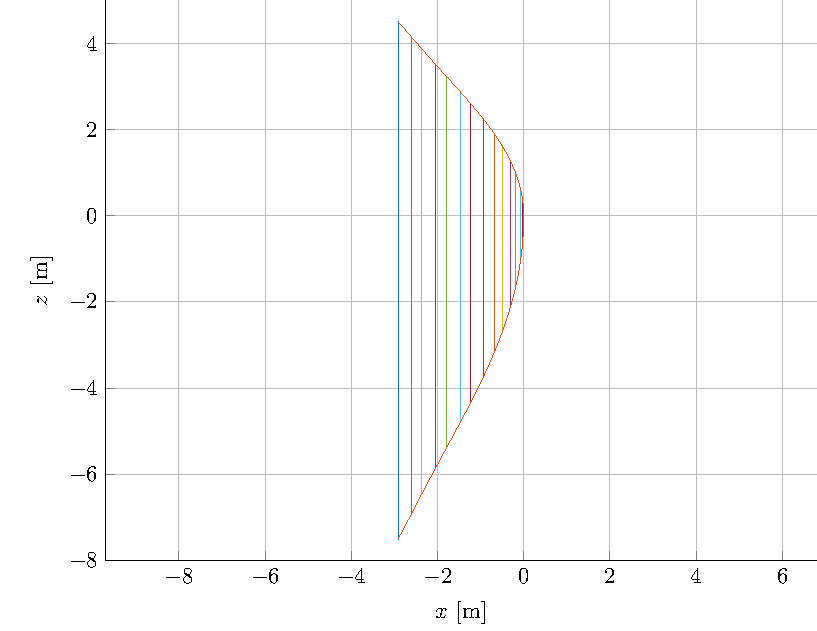
\includegraphics[width=1\textwidth]{./Figure/Aerodynamics/sideview_skewness.pdf}
		\captionsetup{width=0.9\textwidth,skip=-8pt}
		\caption[Side-view of a skewed aerodynamic shape]{Side-view of a skewed aerodynamic shape. The lower part generates a moment around the frontal part of the aeroshell when under an angle of attack}
		\label{fig:skewnessplot}
	\end{subfigure}
	\begin{subfigure}[t]{0.45\textwidth}
		\centering
		\captionsetup{width=0.9\textwidth}		
		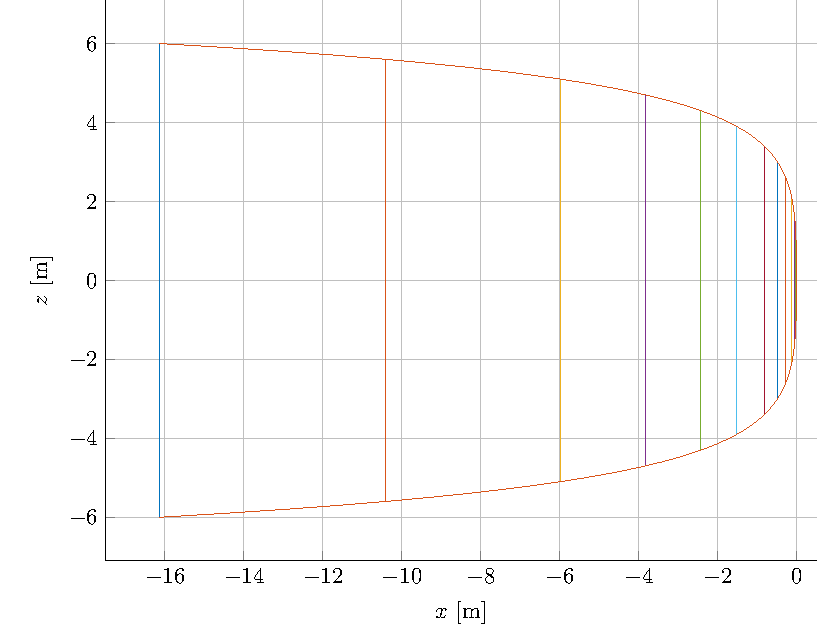
\includegraphics[width=1\textwidth]{./Figure/Aerodynamics/sideview_cmalpha.pdf}
		\caption{Optimised shape resulting in high static stability}
		\label{fig:highcmalphashape}
	\end{subfigure}	
	\caption{Skewed and statically stable aerodynamic shapes}
\end{figure}
	

\paragraph{Various shapes} \label{sec:aeroshapes}
Several large groups of varying shapes can be identified. The relative performance of each group can be qualitatively assessed by looking at the variations of the shape with respect to the optimal shapes for the various parameters. The effect of asymmetric cross-sections will be ignored in this assessment, and will be investigated separately. In Figure \ref{fig:aeroshapes} representative cross sections of the groups can be seen. Group A represents simple concave surfaces. Group B has a concave centre section with a flat ring around it. Group C has an approximately flat central section, with steep edges around the outer radius. Group D represents the half cone shapes, with relatively straight sides and a blunt nose. 

\begin{figure}[h]
	\centering
	
\includegraphics[width=0.5\textwidth]{./Figure/Aerodynamics/AeroShapes.pdf}
	\caption{Various schematic aerodynamic configurations}
	\label{fig:aeroshapes}
\end{figure}

As was discussed in this section, a flat plate will generate the most lift and the most drag, albeit at different angles of incidence. Since Group C closely mimics a flat plate in the majority of its cross-section, it will have the best lift and drag performance. Group B also has a significant flat section and will therefore also have good performance in terms of lift and drag. Groups A and D will both have significant portions of their cross-sections at sub-optimal incidence angles for maximum lift or drag, and will therefore have lower lift and drag performance.

The \gls{sym:cm-alpha} of a given shape is a measure of stability. Shapes which require large moments to change the angle of attack have a higher stability. As can be seen in Figure \ref{fig:CLCD-incidence}, surfaces at incidence angles of 40 to 60 $\left[deg\right]$ provide large changes in force for small changes in angle of incidence. Sections at these incidence angles will therefore stabilise the vehicle, since a change in angle of attack will cause one side of cross section to generate a greater moment than the other. This is visualised in Figure \ref{fig:StabMom}. Cross sections B and C have parts of their cross section at such angles. Since the sections in C are on the outside of the cross section, it will be significantly more stable than type B due to the moment arm these parts have. A and D will have significant portions of their cross sections contribute to the vehicle moment. Although these section are likely to be at sub optimal angles of incidence for high stability, the large area contributing to the stability of the vehicle will ensure that both types of cross section are stable. 


\begin{figure}[h]
	\centering
	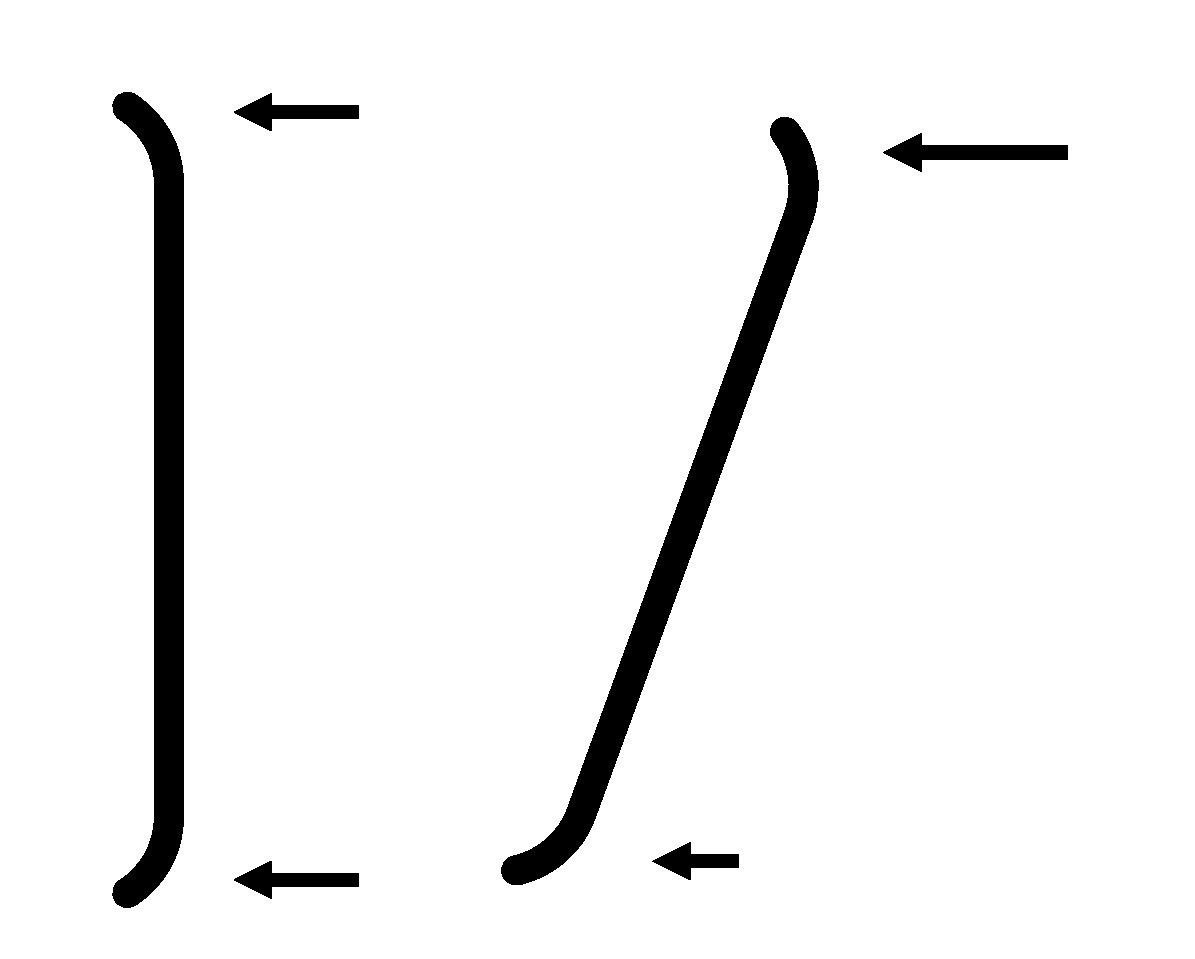
\includegraphics[width=0.5\textwidth]{./Figure/Aerodynamics/StabilizeMoment.pdf}
	\caption{Stabilising effect of reduced incidence angle sections}
	\label{fig:StabMom}
\end{figure}

\paragraph{Asymmetry}
An asymmetric body will ensure that even at zero degrees angle of attack, the vehicle generates lift. As explained in Section \ref{subsec:orbitsens}, this allows for greater control of the vehicle during aerocapture and entry and is therefore desirable. The angle of attack that can be attained is limited by the crew module extending into the flow around the body. Achieving a higher lift at a lower angle of attack is therefore desirable. If the shape is heavily offset to one edge of the body, the crew module will extend into the flow at very low angles of attack. Figure \ref{fig:LDSkew} shows the effect of asymmetry on the lift-to-drag ratio by transforming a given symmetric shape into an asymmetric shape. The asymmetric shapes are created by a linearly shifting the cross sections of the body in the $zy$-plane along the $y$-axis, with no shift at $x=0$ and maximum shift at $x=x_{max}$. 

\begin{figure}[h]
	%\centering
	\hspace{-8mm}
	\setlength\figureheight{0.4\textwidth} 
	\setlength\figurewidth{0.95\textwidth}
	\input{./Figure/Aerodynamics/LoverDplot.tikz}
	\caption{Effect of asymmetric shape on lift-to-drag ratio}
	\label{fig:LDSkew}
\end{figure}


%\subsubsection{Control system sensitivity}\label{subsec:controlsens}
%\subsection{Control}

**Intro**

\subsubsection{Assumptions}

**Primary and Secondary assumptions**

\subsubsection{Trim point}

**Moment equilibrium figures/equations**
**CG-location plot(s)  with conclusion on CG for AoA~20 and sideslip angle=0**

\subsubsection{Stability}

**From E.Mooij**

\subsubsection{Available control systems}

**Intro**

\paragraph{\acrfull{cg} offset}

**Not nessesary for AoA, not feasible for sideslip**

\paragraph{Thrusters}

**Sebstiaan**

\paragraph{Aerodynamic surfaces}

**Guido**





\subsubsection{Thermal sensitivity}\label{subsec:thermalsens}
To investigate the influence of lay-up materials, heat flux variations, vehicle diameter and the trajectory approach on the \gls{tps} a sensitivity analysis is performed. First materials are selected to form multiple lay-ups. The different lay-ups are then optimised for different loading conditions. First the influence of heat flux variations on areal density is investigated. Subsequently, variations in mass due to changing diameters are tested. Lastly, the lay-ups are tested for different trajectories, either with a direct trajectory or with a parking orbit between aerocapture and landing. This investigation is done by using the tool described in Section \ref{subsec:thermaltool} and successfully validated in Appendix \ref{sec:VandVthermo}.

\paragraph{\gls{tps} materials}
Table \ref{tab:tpsmatprop} shows the materials that are used in the inflatable heat shield. A more extensive list of possible \gls{tps} materials and their properties can be found in Appendix \ref{sec:Thermoprop}. These materials have been proposed during the design of multiple inflatable decelerator concepts, such as \gls{irve} and \gls{thor} \cite{Hughes2005}. For each material the thermal conductivity, the density, the specific heat, the maximum operative temperature and if applicable, the emissivity are given. The latter is only applicable to the upper thermal protection layers, because these layers, or heat barriers, will radiate heat into the surroundings.
\newline\newline
A selection is made for the most promising thermal protection and insulation layers. These are Nextel BF-20 and Nicalon for the heat barrier layers. Nextel is a material already used by \gls{nasa} in \gls{irve}. Nicalon is a heavier alternative made up of continuous fibres of silicon carbide (SiC) that can withstand higher temperatures than Nextel up to $2073 \left[K\right]$. Also the emissivity of Nicalon is much higher that Nextel, which allows for more radiation. For the insulation layers these are Pyrogel\textsuperscript{\textregistered} 3350 and Pyrogel\textsuperscript{\textregistered} 6650. With those materials three lay-ups are created such that a comparison can be made between the heat barriers and insulators. A schematic view of the layers is shown in Figure \ref{fig:layersensthermal}. Lay-ups 1 and 2 can be used to compare the performance of Pyrogel\textsuperscript{\textregistered} 3350 and 6650. Lay-ups 2 and 3 serve as comparison for the Nextel BF-20 and Nicalon. These lay-ups will be tested for different heat fluxes as well as different diameters.

\begin{table}[ht]
	\caption {Flexible \acrlong{tps} material properties \cite{Corso2009,Corso2011,DuPont2011,Smith2011,Nye,Zinkle1998}}
	\centering
	\begin{tabular}{|l|l|l|l|l|l|l|}
		\hline
	        \textbf{Material}         & \textbf{ $\mathbf{k}$ $\mathbf{\left[\frac{W}{m\cdot K}\right]} $} & \textbf{ $\mathbf{ \rho }$ $\mathbf{ \left[ \frac{kg}{m^3} \right] }$} & \textbf{  $\mathbf{ c_{p} }$ $\mathbf{ \left[ \frac{J}{kg \cdot K} \right] }$ }& \textbf{ $\mathbf{ T_{max} }$ $\mathbf{ [ K ] }$} &\textbf{ $\mathbf{ \varepsilon }$ $\mathbf{ [ - ] }$} & \textbf{Function} \\[1.6ex]   \hline \hline
		Hi-Nicalon			& 2.4			& 2900	& 1200	& 2073	& 0.93	& rad. \& barrier	\\ \hline
		Nextel BF20			& 0.146			& 1362	& 1130	& 1643	& 0.443	& rad. \& barrier	\\ \hline
		Pyrogel\textsuperscript{\textregistered} 6650		& 0.030			& 110	& 1046	& 923	& -		& insulator			\\ \hline
		Pyrogel\textsuperscript{\textregistered} 3350		& 0.0248		& 170	& 1046	& 1373	& -		& insulator			\\ \hline
		Kapton				& 0.12			& 1468	& 1022	& 673	& -		& gas barrier		\\ \hline
		Kevlar				& 0.04			& 1440	& 1420	& 443	& -		& structural		\\ \hline
		PBO Zylon\textsuperscript{\textregistered}			& 20			& 1540	& 900	& 673	& -		& structural		\\ \hline

	\end{tabular}
	\label{tab:tpsmatprop}
\vspace{-4mm}
\end{table}

\begin{figure}[h]
	\centering
	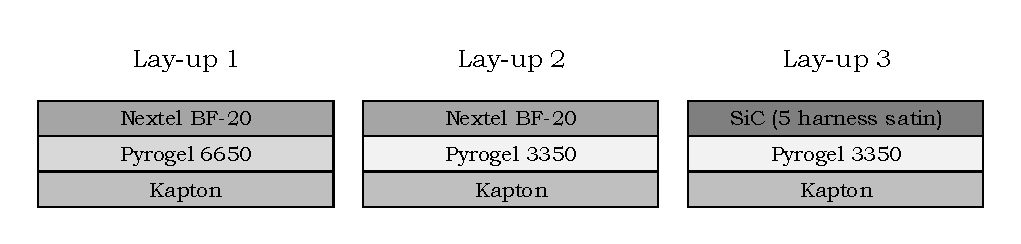
\includegraphics[width=\textwidth]{./Figure/Thermal/layersensthermal.pdf}
	\caption{Tested lay-ups for the sensitivity analysis}
	\label{fig:layersensthermal}
\end{figure}

\paragraph{Effect of heat flux}
In order to analyse areal density performance of lay-ups and changes due to varying atmospheric conditions a heat flux sensitivity is performed. To achieve this, ratios of the heat flux of a possible trajectory are used. The trajectory is found using a diameter of $12 \left[ m \right]$. The results are shown in Figure \ref{fig:sensitivityq}. The horizontal axis shows the heat flux ratio and the areal density is shown on the vertical axis. 

\begin{figure}[h]
	\centering
	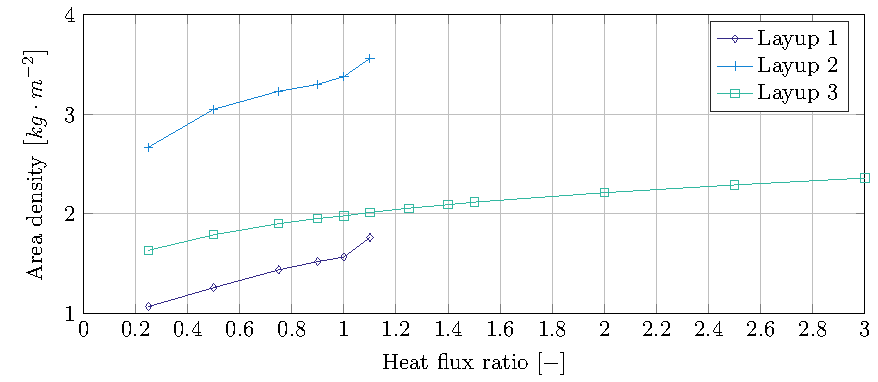
\includegraphics{./Figure/Thermal/Sensitivityq.pdf}
	\caption{Heat flux sensitivity for the three selected lay-ups}
	\label{fig:sensitivityq}
\end{figure}


As expected, the mass of the \gls{tps} increases with increased loading. Secondly and most important, the relative performance of the lay-ups can be observed. Lay-up 1 is clearly the lightest solution, followed by lay-up 3 and 2. Although lay-up 1 performs better in terms of its mass, the amount of loading it can bear is limited. If small changes in atmospheric properties occur during the \gls{edl} phase, for instance due to Martian storms, the \gls{tps} may succumb under the increasing loads. Therefore it is wise to choose Nicalon for further design. Lastly, if lay-up 1 and 3 are analysed relative to each other, it is clear that Pyrogel\textsuperscript{\textregistered} 6650 performs much better than the 3350 variant. Therefore, for further design it is more favourable to use Pyrogel\textsuperscript{\textregistered} 6650 as an insulator. The drawback of Pyrogel\textsuperscript{\textregistered} 6650 is that it has a lower maximum use temperature. This is solved by using a good heat barrier such as Nicalon.

\paragraph{Effect of diameter}
The three lay-ups are put to the test for different diameters. Aerodynamic analysis has provided heat fluxes for trajectories with corresponding diameters of $6$, $9$, $12$, $15$ and $18 \left[ m \right]$. As a side note, because the aerodynamic shape is different from the one in the previous paragraph, Figures \ref{fig:sensitivityq} and \ref{fig:sensitivityA} cannot be directly compared. An increase in heat flux caused an increase in the maximum temperature, surpassing the Nextel operative temperature limit which made it impossible for lay-ups 1 and 3 to fly trajectories at diameters of $12 \left[ m \right]$. Optimising the thickness of the lay-ups for these heat flux result in Figure \ref{fig:sensitivityA}. The solid lines indicate the nominal trajectory, with a parking orbit after aerocapture. For both graphs, the horizontal axis shows the relevant diameters. The plot on the left shows the areal density on the vertical axis and the right plot shows the total mass of the frontal \gls{tps} on this axis.

\begin{figure}[h]
	\centering
	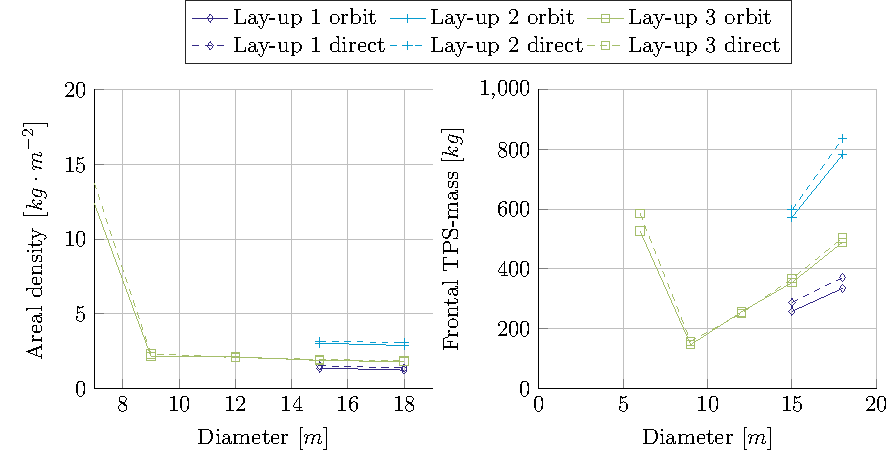
\includegraphics{./Figure/Thermal/SensitivityA.pdf}
	\caption[Areal sensitivity for the three selected lay-ups]{Areal sensitivity for the three selected lay-ups, both for a direct trajectory and a usual trajectory with a parking orbit after aerocapture. Left plot shows areal density, whereas the right plot shows the total mass.}
	\label{fig:sensitivityA}
\end{figure}

For increasing diameters, larger radii of curvature can be obtained, resulting in a direct decrease of incoming heat flux. Also, due to the increasing diameters which causes an increase in \gls{sym:CD} and a reduction in ballistic coefficient, the vehicle can decelerate by the same amount at lower dynamic pressures. Therefore, the vehicle can stay higher in the atmosphere and fly in thinner air with the same velocity, decreasing heat development and incoming heat flux.\\

This effect can clearly be seen in the left figure, where the areal density decreases for increasing diameters. Obviously more material must be used to create larger \gls{tps}, which mostly results in a total mass increase for larger diameters. This can be seen in the right figure. The only exception is lay-up 2, the lay-up that is able to cope with the larger incoming heat flux at lower diameters. An optimum of its thermal performance is found at $9 \left[ m \right]$ where the frontal \gls{tps} mass reduces to approximately $150 \left[ kg \right]$. In addition, the relative mass performance of the different lay-ups is comparable to the performance in the previous paragraph.

\paragraph{Effect of time}
Whenever the vehicle is changing its descend rate, the total dissipated energy is still the same. However, the energy rate profile will have a different distribution over time, changing the temperature throughout the \gls{tps}. Steeper descends require a thicker heat barrier, limiting the heat flow to the rest of the shell, such that operational temperature of the insulator is not exceeded. A more gradual descend increases the time spend in the atmosphere and therefore increases the heat stored in the heat shield. This puts limits on the insulators minimum thickness, to block the heat flow to the structural layers and the rest of the vehicle. Therefore, the effect of descent time is analysed. The results are also shown in Figure \ref{fig:sensitivityA}. An alteration in time is visible by considering two types of viable trajectories, a direct trajectory and one with an orbit after aerocapture. From the figure it can be seen that the direct trajectory is the limiting one.

\subsubsection{Structural sensitivity}\label{subsec:strucsens}
\paragraph{Inflatable structural mass}

Based on the mass estimation model outlined in subsection \ref{subsec:structool}, the effect of changing design parameters on inflatable structural mass is investigated hereafter. To this end, the following design parameters have been investigated: centerbody and inflated diameter, half-cone angle, the number of toroids and aerodynamic loading. The drag coefficient has not been investigated separately, for it appears exclusively multiplied by dynamic pressure and a percentual increase in drag coefficient therefore has the same effect as an equal percentual change in dynamic pressure. The product of these two terms gives the aerodynamic force working over the decelerator frontal surface area.

\begin{figure}[ht]
	\centering

	\begin{subfigure}[b]{0.49\textwidth}
		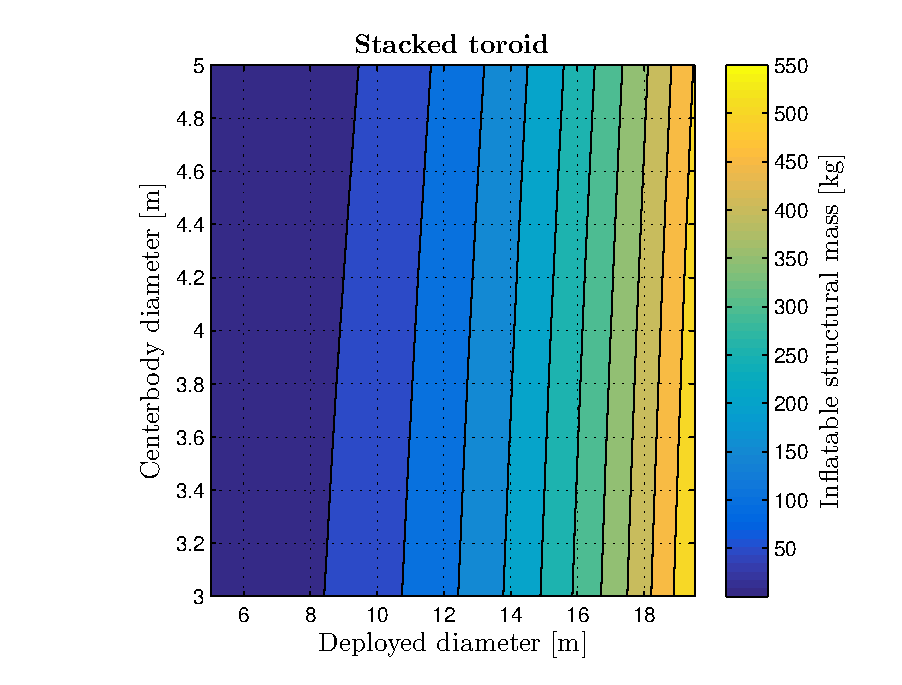
\includegraphics[width=0.96\textwidth]{./Figure/Structure/diameters_test.eps}
		\caption{Mass versus centerbody and deployed diameter}
		\label{fig:diameters_strucmass}
	\end{subfigure}
	\begin{subfigure}[b]{0.49\textwidth}
		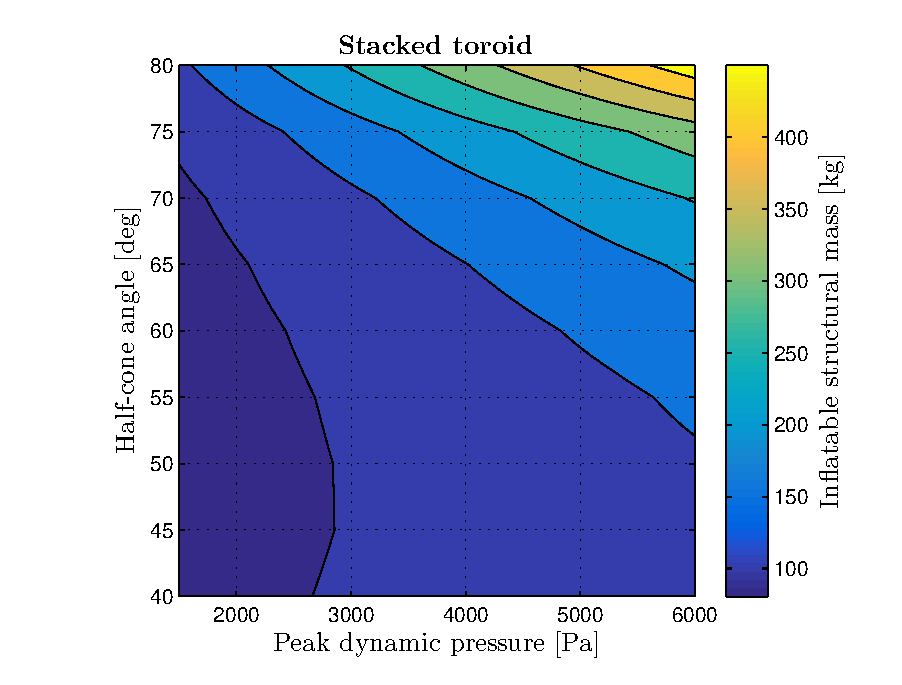
\includegraphics[width=0.96\textwidth]{./Figure/Structure/halfcone_test.eps}
		\caption{Mass versus half-cone angle and peak dynamic pressure}
		\label{fig:halfcone_strucmass}
	\end{subfigure}
	\begin{subfigure}[b]{0.49\textwidth}
		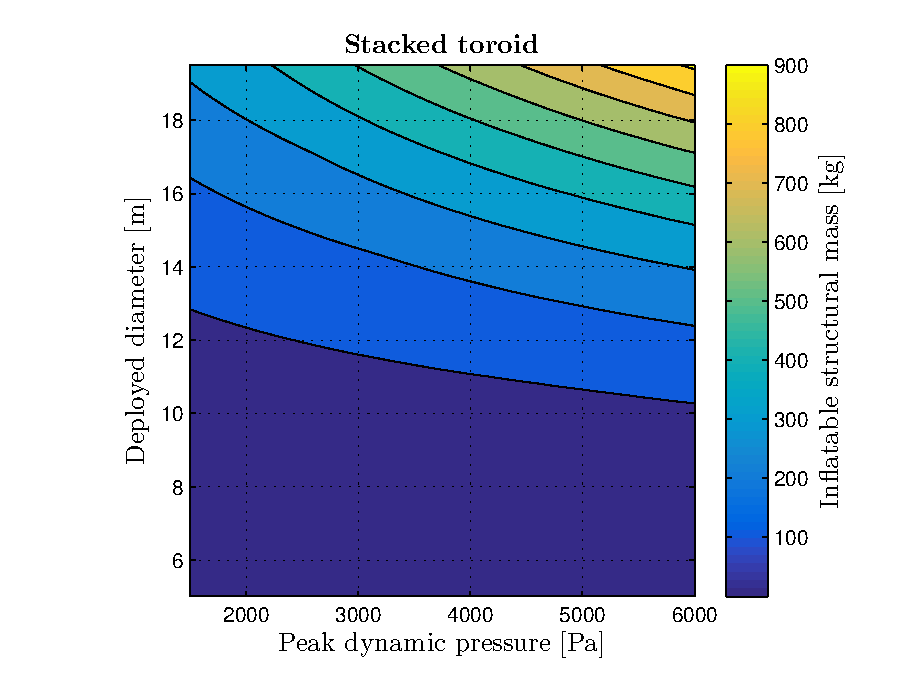
\includegraphics[width=0.96\textwidth]{./Figure/Structure/pressure_test.eps}
		\caption{Mass versus deployed diameter and peak dynamic pressure}
		\label{fig:press_strucmass}
	\end{subfigure}
	\begin{subfigure}[b]{0.49\textwidth}
		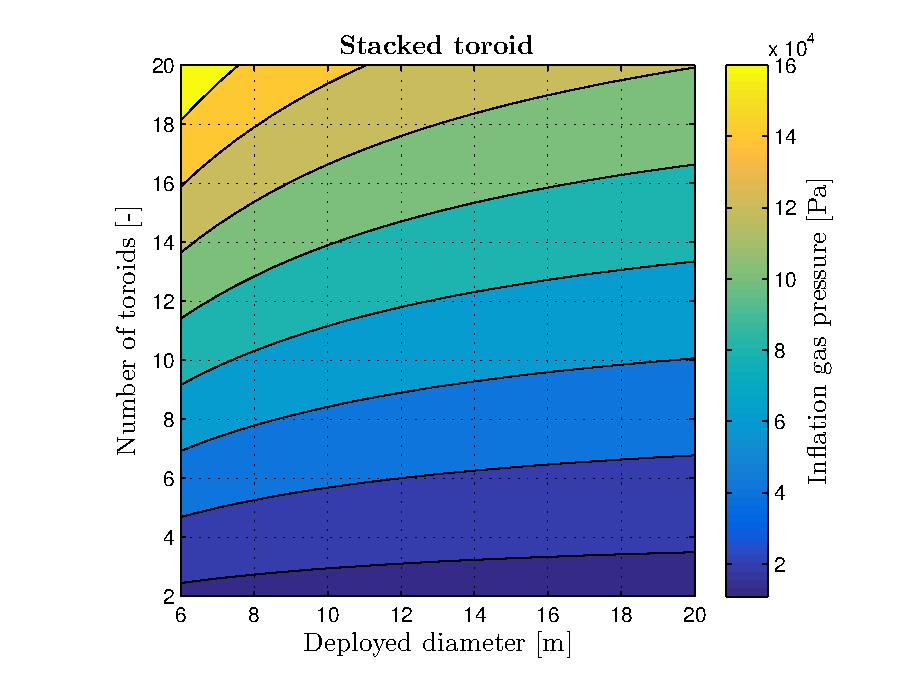
\includegraphics[width=0.96\textwidth]{./Figure/Structure/inflation_test.eps}
		\caption{Inflation pressure versus number of toroids and deployed diameter}
		\label{fig:inflpress_strucmass}
	\end{subfigure}
\caption{Inflatable structural mass and inflation pressure as a function of design parameters}
\end{figure}
Firstly, from Figure \ref{fig:diameters_strucmass} it follows that mass decreases with an increasing centerbody diameter given a deployed diameter. This is due to the fact that an increasing centerbody diameter increases the areal contribution of the centerbody: the inflatable requires less structural mass by decreased aerodynamic loading thereof, as aerodynamic pressure works over an area. In turn, this suggests that the centerbody becomes heavier, which is not the case as the centerbody is typically sized for launch rather than (re-)entry loads \cite{Lindell2006}. It can therefore be concluded that maximizing centerbody diameter is beneficial for structural mass. 

Secondly, from Figure \ref{fig:press_strucmass} it follows that increasing dynamic pressure effects an increase in structural mass of the inflatable. This is the result of an increased aerodynamic loading and therefore structural taxation of the inflatable. To withstand this loading, extra structural mass is required. Moreover, for a given peak dynamic pressure an increase in deployed diameter effects an increase in structural mass. Primary cause hereof is the fact that pressure works over a surface area and an increase in area thereby increases the loading. This is further amplified by an increase in bending moments by the larger distance from tip to root.

From Figure \ref{fig:halfcone_strucmass} it may be observed that the half-cone angle significantly affects inflatable structural mass: in general smaller half-cone angles are preferable. Increasing half-cone angle beyond an optimum region at approximately 45 degrees strongly increases structural mass; decreasing it below this region similarly increases structural mass, but less strongly. Moreover, as aerodynamic loading is increased the optimum region shifts and smaller half-cone angles are preferable. This is due to the fact that decreasing the half-cone angle increases bending stiffness by an increased moment of inertia in the bending plane. This increased bending stiffness is further amplified by the three-dimensionality of the sphere cone and carries over to more effective use of material in bending, requiring less mass to resist the bending moment by aerodynamic loading. For a given deployed diameter, however, decreasing the half-cone angle increases the effective inflatable length. This addition of material is to be traded off against the increased bending material. At low dynamic pressures, increased bending stiffness is less warranted than at higher pressures, at which bending loads increase and bending stiffness is increasingly more warranted.

In Figure \ref{fig:inflpress_strucmass} inflation gas pressure is observed to increase for an increasing number of toroids and to decrease with an increasing deployed diameter. Both an increase in the number of toroids and a decrease in deployed diameter decrease toroid radii, effecting an increase in the working area of the inflation pressure. Due to the proportionality of the running load induced by inflation pressure via Equation \ref{eq:Pmin} with toroid radius, a larger inflation pressure is required to induce the same running load with a smaller radius. This running load is based on the consideration that the work done by inflation gas and external forces in axial direction are equal \cite{Brown2009}, independent of the number of toroids. It is similarly independent of the deployed diameter, since both inflation and aerodynamic pressure have the same working area in axial direction.
%The thickness required increases with decreasing material ultimate strength, which explains the differences in structural mass observed between different materials at low dynamic pressures. These differences carry through as loading is increased, where materials with a higher specific strength require less mass to withstand the loading. The material used in \gls{irve}-3, PBO Zylon, is observed to offer notable mass advantages over heritage aramid fibers, such as Kevlar. Mass reduction beyond this level is possible by using Technora and Spectra 2000. All materials are selected based on their operating temperature since these are required to operate in an environment with significant thermal loading. A summary of material properties is given in the Mid-Term Report \cite{Balasooriyan2015b}.
The number of toroids was observed to have no significant effect on structural mass beyond ten toroids, after which mass reductions were found to be within two percent. An increase in the number of toroids from two to ten yields significant mass advantages of up to ten percent. 



Material selection has a significant effect on flexible material mass, as illustrated by Figure \ref{fig:mat}. It can be observed that, for peak dynamic pressures below 2 [$kPa$], minimum gage thickness is leading for all selected fibres. Below this pressure, density is the leading parameter and a less dense material will perform better. Due to the significantly lower density of Spectra 2000, 970 [$kg \cdot m^{-3}$], versus that of for example PBO Zylon, 1540 [$kg \cdot m^{-3}$], Spectra 2000 offers mass advantages at low dynamic pressures. Therefore it can be concluded that for low dynamic pressures materials should be selected based on minimum gage thickness, but thickness rapidly increases as loading is increased and the minimum gage thickness is exceeded. For PBO Zylon, this occurs at a relatively high peak dynamic pressure of 3.5 [$kPa$].

For higher dynamic pressures, materials with a higher specific strength perform better in terms of structural mass. Flexible material is fully loaded in tension by the inflation pressure is required not to fail under tension, dictated by ultimate strength. To this end, a certain thickness with a corresponding mass is required. Mass performance is then directly linked to specific strength and this is confirmed by Figure \ref{fig:mat}. Aramid fibres Kevlar and Technora have the lowest specific strengths, approximately 2 [$MNm \cdot kg^{-1}$]. A notably higher specific strength of 3.44 and 3.77 [$MNm \cdot kg^{-1}$] is attained by Spectra 2000 and PBO Zylon respectively. This confirms the choice for PBO Zylon for its mass advantages over Kevlar in \gls{irve}-3 \cite{Dillman2012a}. Spectra 2000 is capable of achieving a lower mass than PBO Zylon despite its lower specific strength, due to its low density. 

Mass differences between materials remain limited, up to 30 [$kg$] over a range of half-cone angles and diameters.

All materials have been selected based on their operating temperature since these are required to operate in an environment with significant thermal loading. As an example, Spectra 2000 fibres are not deemed suitable for their allowable temperature of 150 degrees Celsius, which would incur significant extra \acrfull{tps} mass. Dyneema would similarly be unsuitable by its temperature limit of 145 degrees Celsius\footnote{URL:\url{http://eurofibers.com/fibers/dyneema/}. Accessed: 17-06-2015} A summary of material properties is given in the Mid-Term Report \cite[p.64]{Balasooriyan2015b}. 

\begin{figure}[ht]
	\centering
	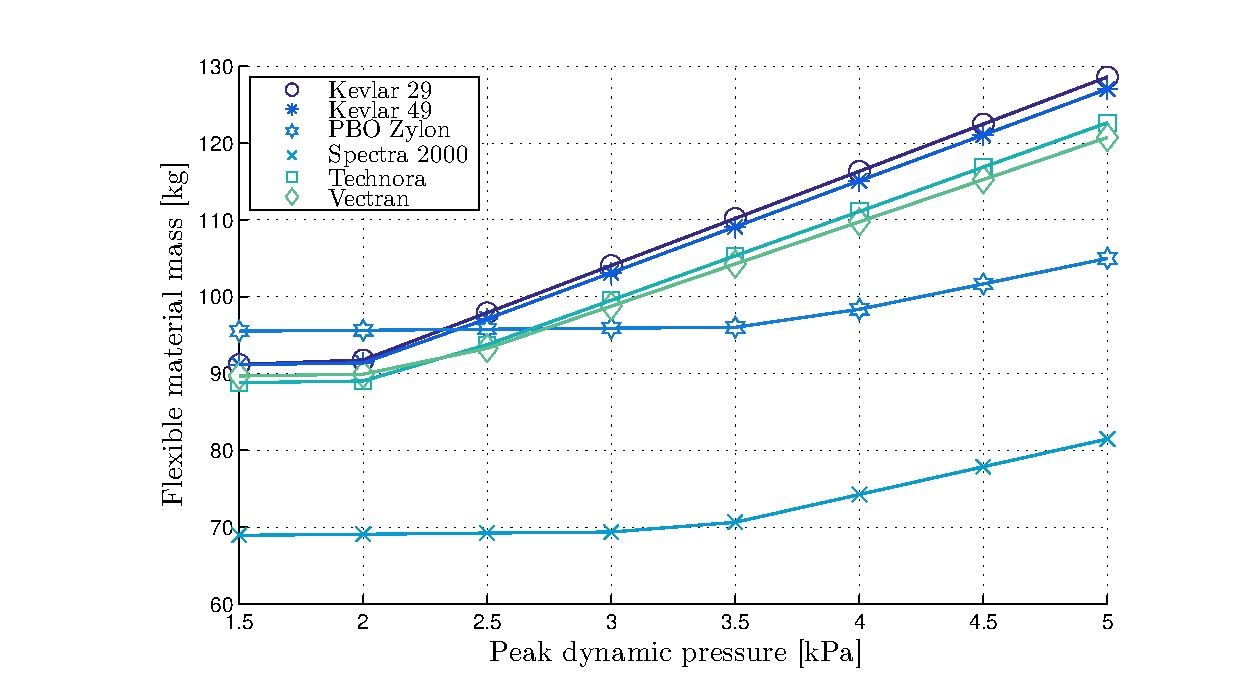
\includegraphics[width=1.0\textwidth]{./Figure/Structure/material_test2.eps}
	\caption{Flexible material structural mass estimation for different materials}
	\label{fig:mat}
\end{figure}

\paragraph{Forces}

Using the force estimation tool for the inflatable structure the sensitivity for the scaling of loads can be determined. Figure \ref{fig:forces} displays the estimated structural loads throughout the inflatable for a total of 9 toroids and a set outer diameter of 12 and 18 [$m$]. The loads as displayed in Figure \ref{fig:forces} feature solely the loads induced by aerodynamic pressure. The internal pressure loads follow separately. This sensitivity analysis is performed to evaluate the scalability of the \gls{hiad} design. Previous \gls{hiad} designs, most predominantly the \gls{irve} missions, feature smaller mission payloads and corresponding smaller diameters. Up to this point the highest diameter stacked toroid design flown is featured in the second and third \gls{irve} missions, namely an outer diameter of 2.93 [$m$]. 

\begin{figure}[ht]
	\centering
	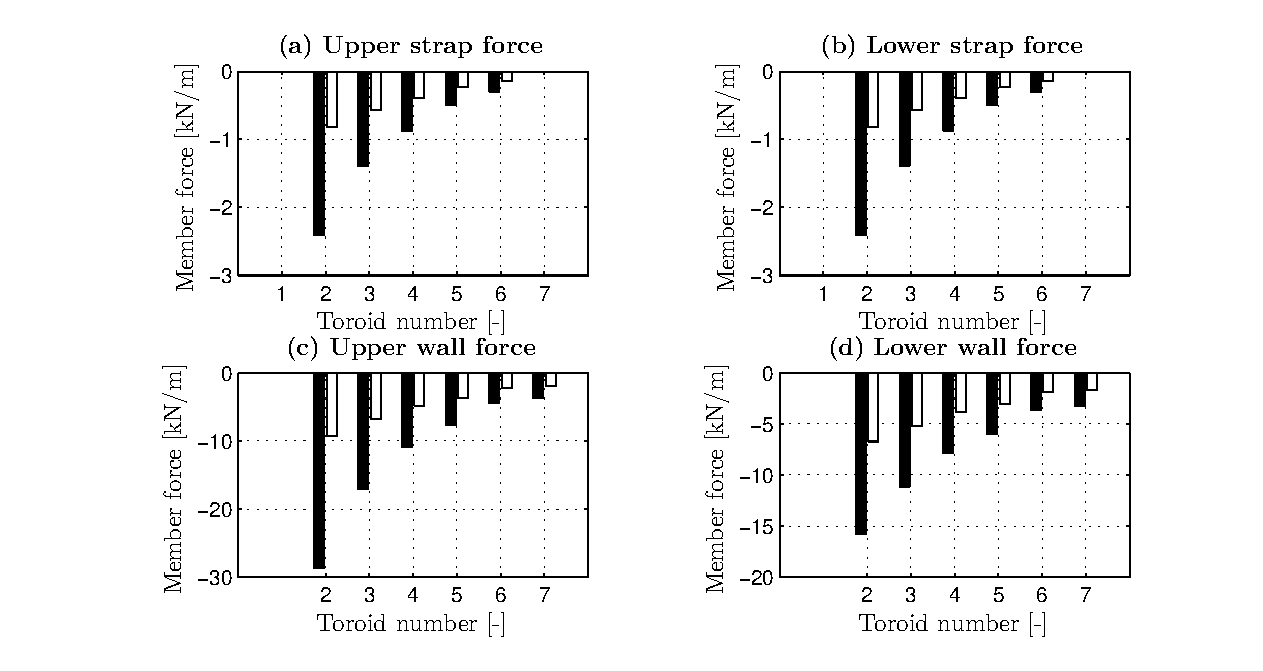
\includegraphics[width=0.9\textwidth]{./Figure/Structure/forces_nopress_test.eps}
	\caption[{Internal force estimation for dynamic pressure 3750 [$Pa$], no inflation pressure applied}]{Internal force estimation for dynamic pressure 3750 [$Pa$], no inflation pressure applied. Black bars are for a diameter of 18 [$m$]; white bars for a diameter of 12 [$m$]}
	\label{fig:forces}
\end{figure}

\begin{figure}[ht]
	\centering
	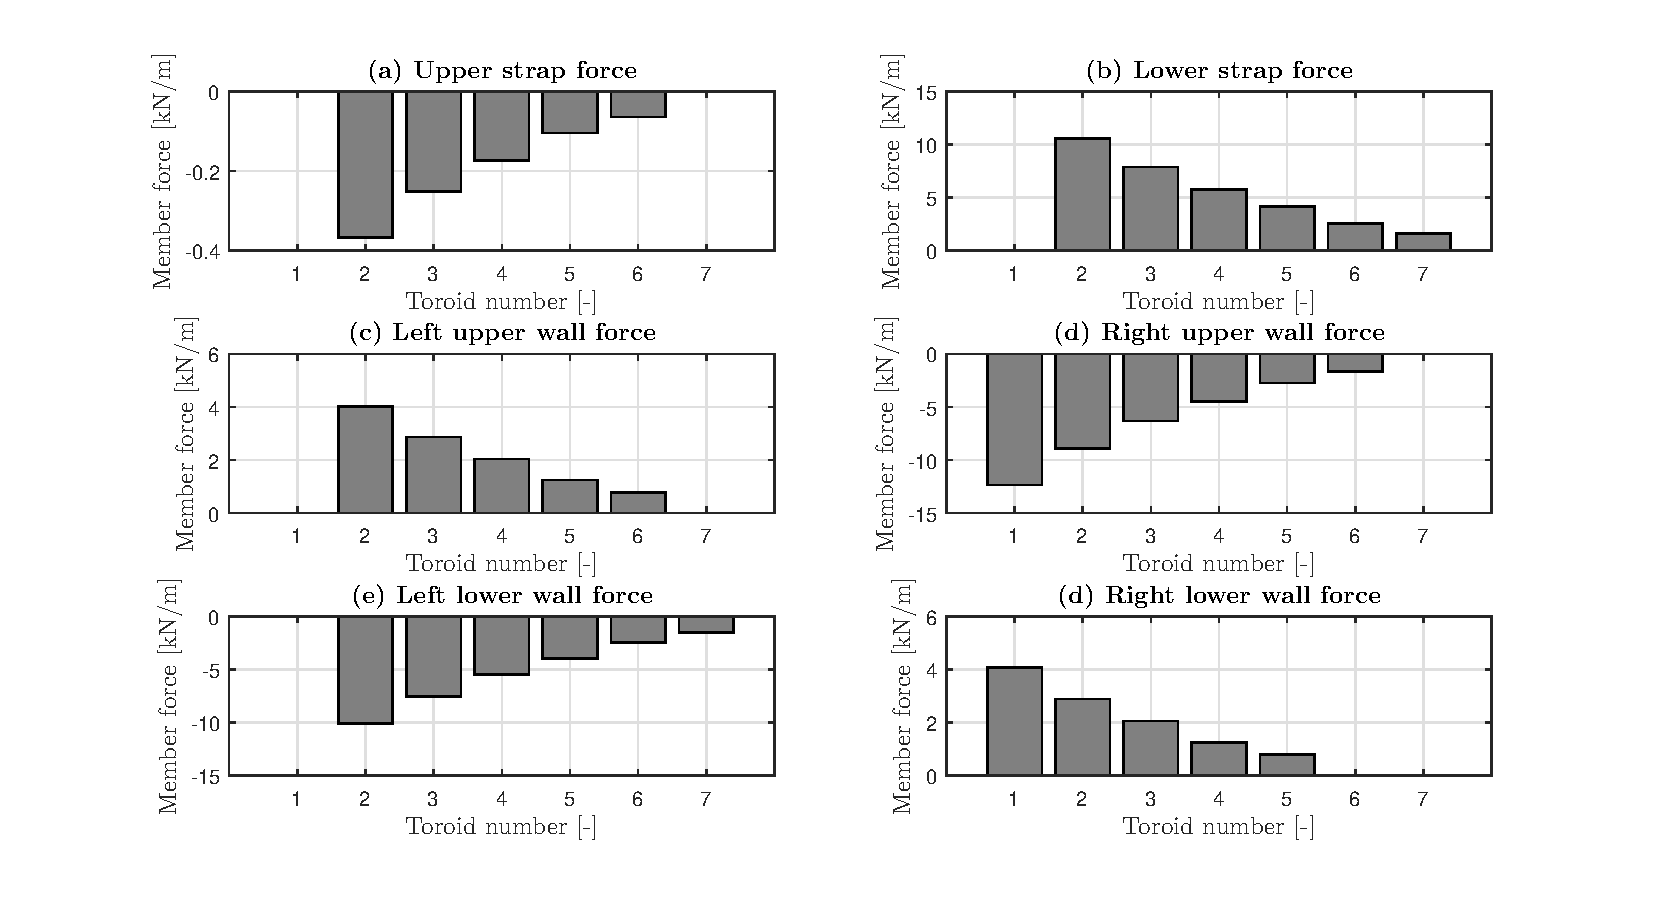
\includegraphics[width=0.9\textwidth]{./Figure/Structure/forces_test.eps}
	\caption[{Internal force estimation for dynamic pressure 3750 [$Pa$], with inflation pressure applied}]{Internal force estimation for dynamic pressure 3750 [$Pa$], with inflation pressure applied. Black bars are for a diameter of 18 [$m$]; white bars for a diameter of 12 [$m$]}
	\label{fig:forcesp}
\end{figure}

From the results of Figure \ref{fig:forces} several conclusions can be made. Most importantly it shows that scaling of the inflatable is possible. Although a load increase can be observed for increasing diameter, this follows only from the additional axial loads. The induced bending moment is not represented in Figure \ref{fig:forces} as this is carried circumferentially. This followed from the verification and validation procedures explained in more detail in Appendix \ref{sec:VandVstruc}. Moreover, loads are found to be within material capabilities.

Secondly the loads do not increase linearly over the diameter. This is the result of the scaling of the loads, to account for the decreasing circumference over which forces act. The reducing diameter causes an additional increase of the loads per unit length.

Thirdly the dynamic pressure loads of Figure \ref{fig:forces} are found to be of a similar order as the internal pressure loads induced per Equation \ref{eq:Q} at the root of the inflatable. Moving towards the tip of the inflatable these differences increase as the internal pressure loads are maintained whereas the loads induce by the dynamic pressure reduce towards the tip. This is further expanded upon in Figure \ref{fig:forcesp} in which pressure loads are included.

The final conclusion with regards to scalability of the inflatable can be made on the basis of Figure \ref{fig:forcesp}. If the internal and external pressure loads are combined a minimum required thickness can be computed on the basis of requiring the structure not to yield. This parameter is relevant as foldability of the inflatable has to be considered as well. Foldability is an important parameter as the inflatable has to be stowed away during launch and the transfer towards Mars. From this yielding criterion and a typical material such as Kevlar 49 a minimum required thickness of below 0.01 [$mm$] is found. Since this value is rather small the thickness of the inflatable is not a consideration from a folding perspective even for large diameters.







\section{Final design}\label{cha:finaldesign}

\subsection{Iteration process} \label{sec:iterationprocess}
In order to structure the design process, several design aspects were separated to facilitate  iterating over the design. The goal is to find a design that complies with the requirements as given in Section \ref{sec:reqbreak}. This is done by choosing a design concept containing a combination of an aerodynamic shape, trajectory, \gls{tps}, inflation structure and control system and analysing its performance. After that, the analysis of the concept is used to assess possible points of improvement if the requirements are not yet met. This is repeated until all requirements are complied with. The design process is started with an initial design which is assessed for its performance which is then used as a baseline.

The aerodynamic shape is chosen such that certain aerodynamic properties are achieved. This is largely done by optimisation since this allows a high fidelity in design optimisation objectives and constraints. These aerodynamic properties are chosen based on the previous design analysis. 
When a suitable design is chosen, the resulting aerodynamic characteristics are used in determining a trajectory that complies with the initial and final velocity and height requirements. This is done by choosing a bank angle profile, choosing the bank angle as a function of time to arrive at the required location and velocity. 
The trajectory data containing velocity, density, Mach number and dynamic pressure is used for the inflation structure sizing, \gls{tps} lay-up and control system mass estimation. The shape and maximum dynamic pressure in the trajectory is used in determining the inflation structure, for which a parametric mass model is used to estimate the decelerator mass. 
Also, a representative truss structure is used to determine whether the loads don't exceed the material maximum loads. The heat flux into the system, which in turn amounts to a temperature distribution through the structure and through time, is calculated with the trajectory data. Numerically integrating the 1D heat equation with as input the heat flux data yields a temperature distribution for a given lay-up. The lay-up is then iterated until no layer temperature exceeds its maximum temperature while having the smallest thickness possible such that the \gls{tps} has the lowest possible mass. 
The control system mass is finally estimated using the required bank angle through the trajectory and moments of inertia.

When the technical analysis of the concept is done, the iteration is completed by analysing the results and assessing points where improvement can be made. When not all requirements are met, changes have to be made tot he design. Several problems have been identified during the design phase:
\begin{itemize}
	\item In the case the temperature in the different \gls{tps} layers become too high, even for high thicknesses, the orbit needs to be changed to facilitate a lower maximum dynamic pressure. This can be done by choosing the lowest point of atmospheric entry higher such that the density is lower. If achieving orbit at this higher point is not possible with the current aerodynamic design, the drag coefficient is to be increased to allow the same deceleration at lower dynamic pressures.
	
	\item If the thermal protection system mass or inflation structure mass makes the total design exceed the mass requirement, also the maximum dynamic pressure is to be decreased such that physical loads on the structure and thermal loads on the \gls{tps} are decreased.
	
	\item If bank angle control does not perform well enough to allow a trajectory that satisfies the requirements, the lift over drag ratio can be increased to allow more freedom in trajectory choice.
	
	
\end{itemize}

The iteration strategy is visualised as a flow-chart in Figure \ref{fig:iterativedesignflowchart}. In this figure the solid lines represent design information flowing towards the areas that still need analysis. In the `Design within requirements?' decision box, the check is made whether the mass is within budget and the temperature does not exceed the maximum temperature of the material. If this is the case, the design meets the requirements and is thus the acceptable choice.




\begin{figure}[h!]
		\vspace{-1cm}
		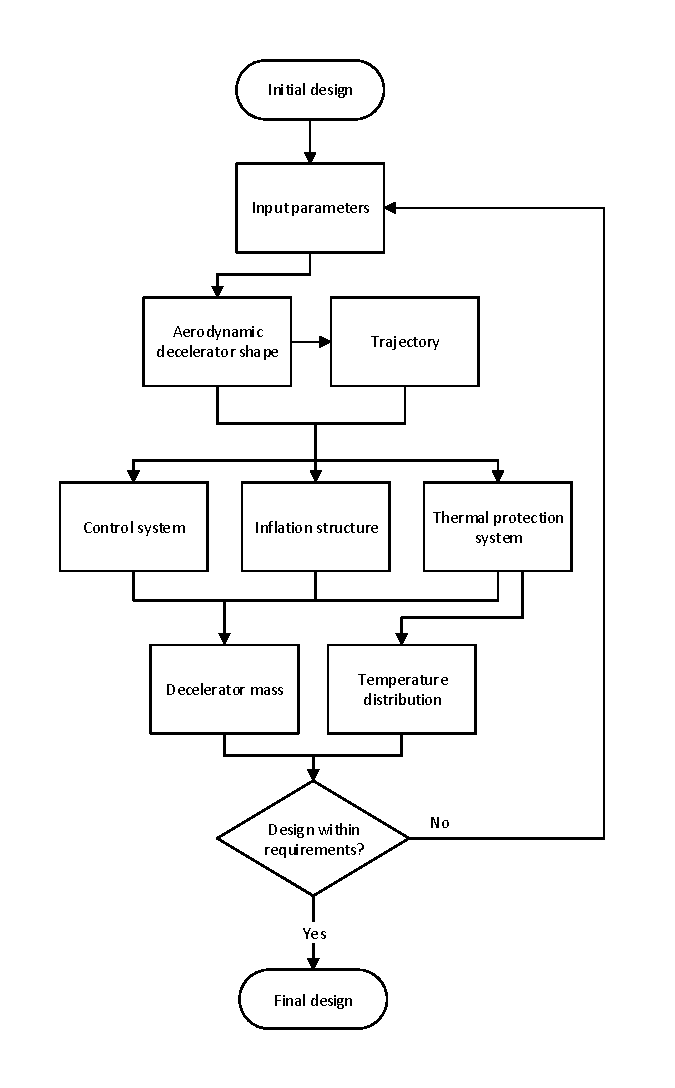
\includegraphics[width=0.8\textwidth]{./Figure/DesignIterationPhilosophy_new.pdf}
		
		\caption{The iterative design process flowchart}
		\label{fig:iterativedesignflowchart}
\end{figure}

\subsection{Trajectory design} \label{sec:trajectorydesign}
In this section the design of the trajectory followed by the spacecraft during the mission is presented. Also the motivation behind it, its sensitivity to changing atmospheric properties and the possibility to correct for these changes are explained. The main input with which the trajectory is calculated is the shape of the decelerator. This shape and the reasoning behind it is presented in Section \ref{subsec:infldes}. An overview of the mission trajectory is given in Figure \ref{fig:trajectory}.

\begin{figure}
	\centering
	
	\begin{subfigure}[b]{0.7\textwidth}
		\vspace{-22mm}
		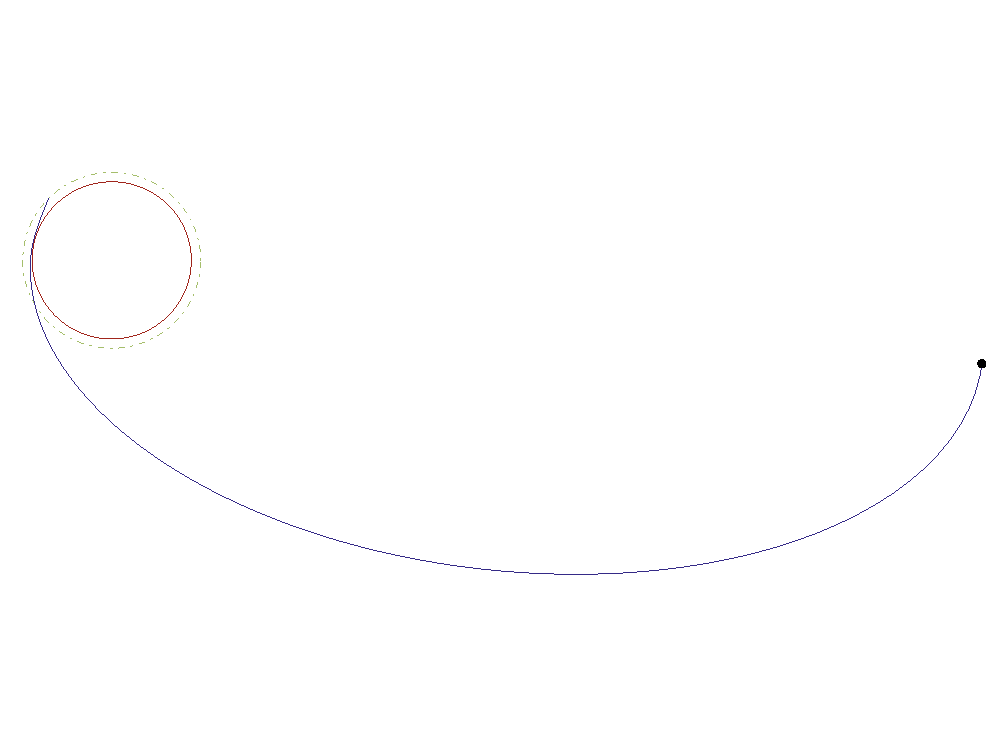
\includegraphics[width=\textwidth]{./Figure/Orbit/aerocapture_trajectory.pdf}
		\vspace{-25mm}
		\caption{The aerocapture trajectory visualised}
		\label{fig:capture_trajectory}
	\end{subfigure}
	\begin{subfigure}[b]{0.7\textwidth}
		\vspace{-10mm}
		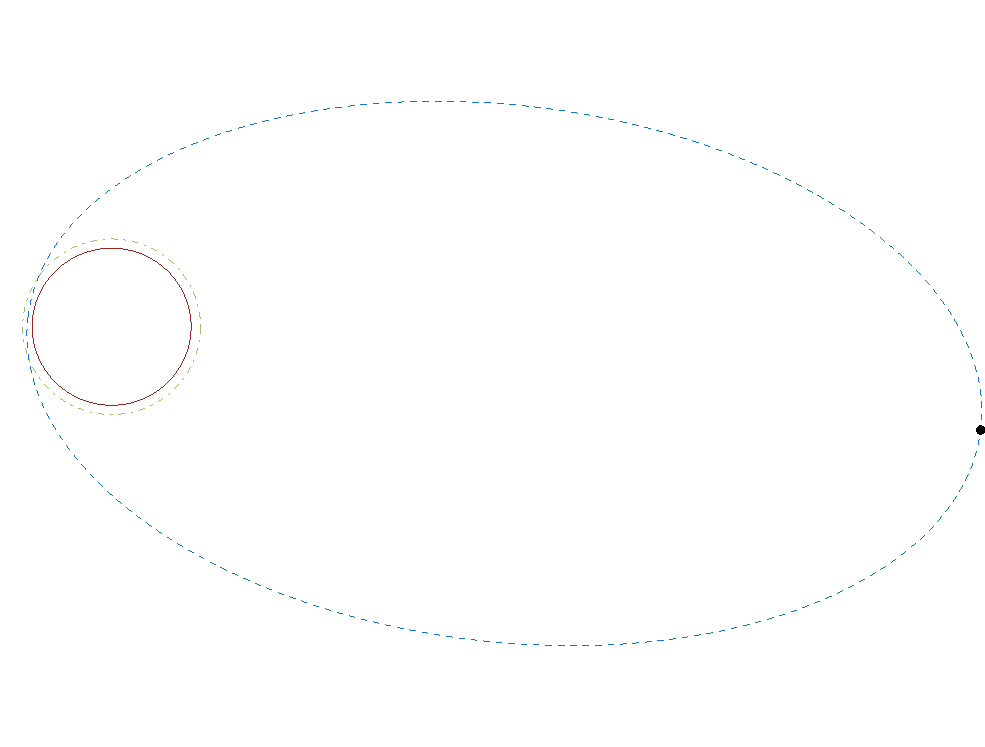
\includegraphics[width=\textwidth]{./Figure/Orbit/parking_trajectory.pdf}
		\vspace{-15mm}
		\caption{The parking orbit after the orbit raise}
		\label{fig:parking_trajectory}
	\end{subfigure}
	\begin{subfigure}[b]{0.7\textwidth}
		\vspace{-22mm}
		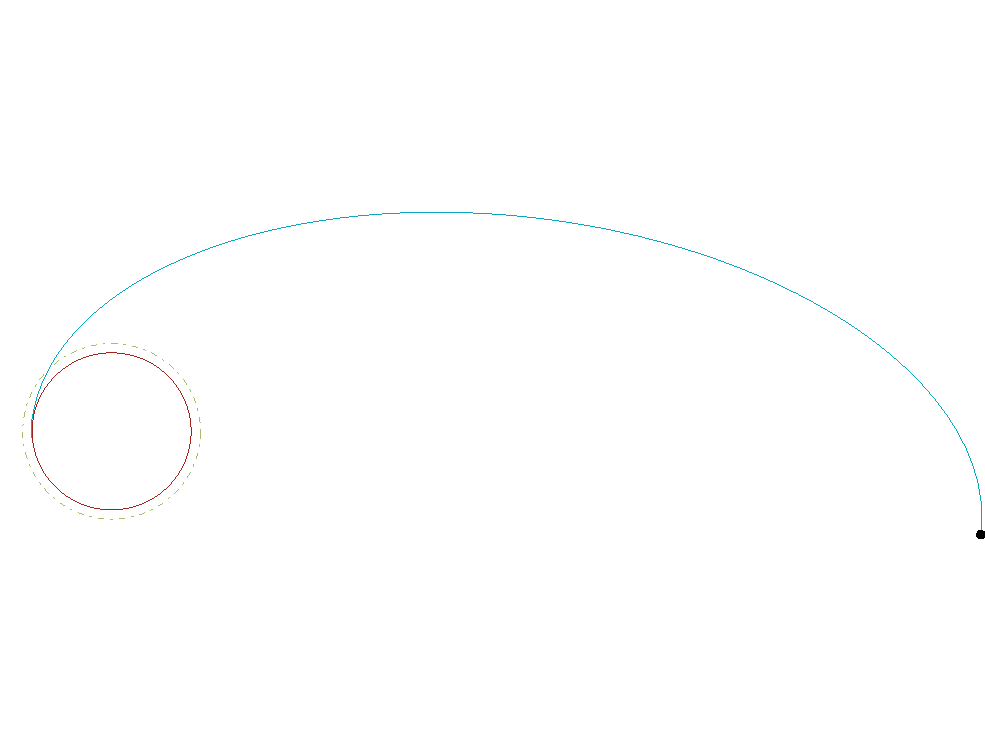
\includegraphics[width=\textwidth]{./Figure/Orbit/re-entry_trajectory.pdf}
		\vspace{-25mm}
		\caption{The re-entry trajectory after lowering the orbit}
		\label{fig:re_entry_trajectory}
	\end{subfigure}
	\caption[Visualisation of the spacecraft trajectory]{Visualisation of the spacecraft trajectory. The apoareion is shown with a black dot}
	\label{fig:trajectory}
\end{figure}

\subsubsection{Aerocapture} \label{sec:aerocapture}
The first phase of the trajectory is aerocapture, in which the objective is to lose enough energy to get in a Mars synchronous orbit. The velocity that has to be obtained at the end of aerocapture in order to get in such an orbit is $4.53 \left[km \cdot s^{-1}\right]$. In Figure \ref{fig:orbit_aerocapture_data} it can be seen from the velocity profiles that they all end at this velocity.

Furthermore the trajectory was chosen as high through the atmosphere as possible to lower the required \gls{tps} and structural masses. A pass higher through the atmosphere decreases both the heat flux and peak dynamic pressure which are used to design the \gls{tps} and inflatable structure respectively.

These two objectives are conflicting since a higher altitude corresponds to a lower density, which makes it harder to achieve the required velocity change. In order to still reach the desired velocity, two options are available: with a longer aerocapture, the lower deceleration at higher altitudes is applied for enough time to reach the final velocity, and with a higher drag coefficient or frontal area the aerodynamic deceleration is increased for equal dynamic pressures.

A longer aerocapture can be achieved by improved control over the vehicle, which is accomplished by a higher lift coefficient. A longer aerocapture however, increases the total heat load, which may lead to a higher \gls{tps} mass.

In order to facilitate both objectives for aerocapture it is thus important that the aerodynamic shape has a high lift-to-drag ratio as well as a high drag coefficient. For the entry and descent phase conflicting objectives for the shape are found since a lower drag coefficient is required such that more time is available in this phase to manoeuvre. In Section \ref{sec:trajectory_summary} a conclusion is drawn on the properties needed from the design of the aerodynamic shape.

In Figure \ref{fig:orbit_aerocapture_data} the parameters that were recorded during the simulation are shown for the nominal trajectory and two trajectories created for a $10\%$ increase and decrease in atmospheric density. This change in density is based on the maximum estimated error in the \gls{esa} Mars climate database v5.2 \cite{Lewis2015}.

The bank control profile for the trajectories can be changed, by varying bank angle and timing, to attain the same exit velocity for each atmospheric density. This exit velocity is needed to get into a Mars synchronous orbit. The fact that a bank control profile is available for each density proves that a density change of $\pm 10\%$ can be accounted for. However, some other parameters of the trajectory do change. The peak acceleration and dynamic pressure increase for a higher density. The \gls{tps} and inflatable structure should be sized on the worst case. Also the time passed and the position of exit (defined by $\tau$ in Figure \ref{fig:angles}) are different for each trajectory. These changes have a significant effect on the entry and descent phase. This effect will be explained in Section \ref{sec:entry_descent}.

\begin{sidewaysfigure}
	\centering
	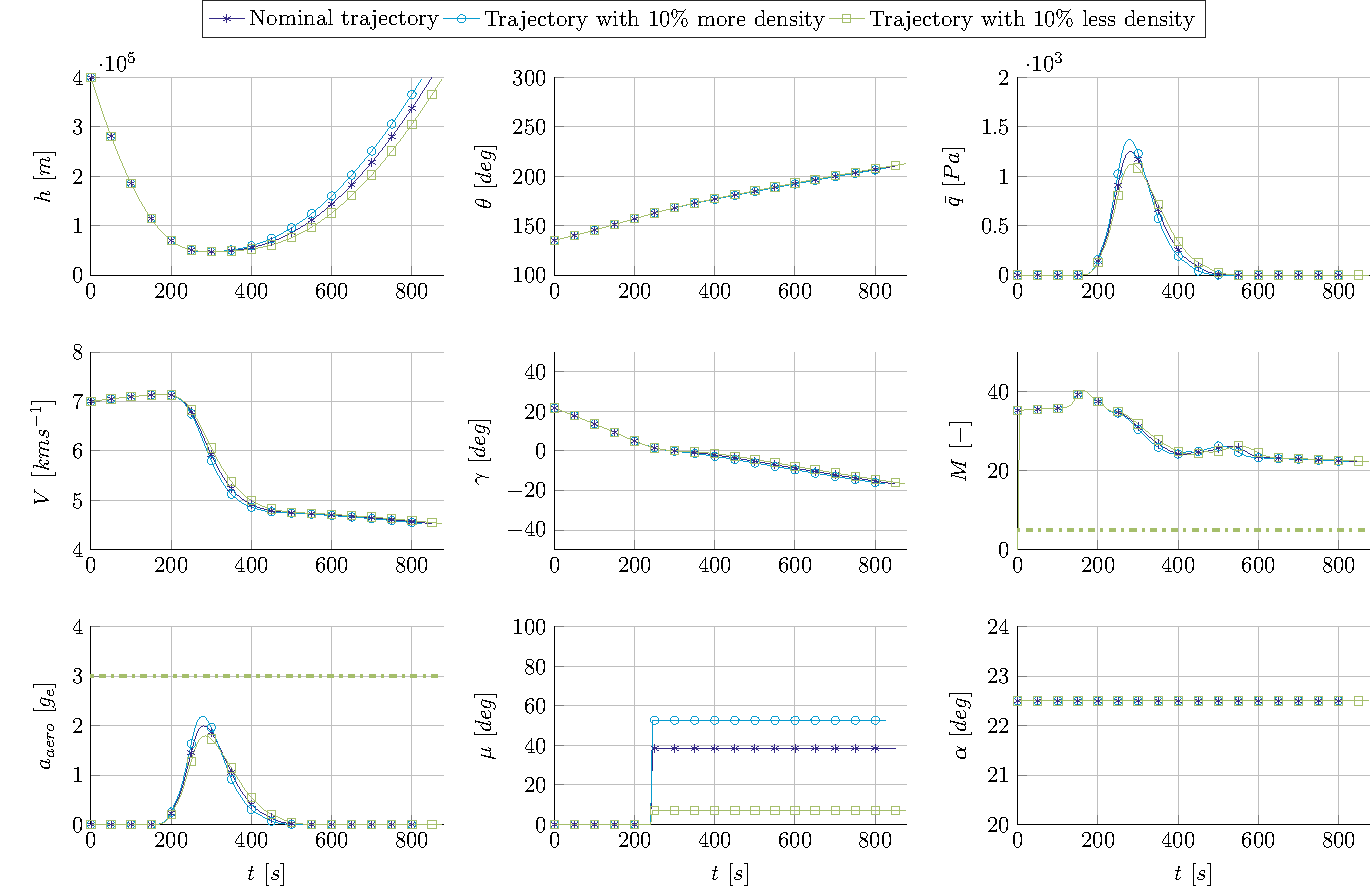
\includegraphics[width=0.99\textwidth]{Figure/Orbit/sensitivity_aerocapture.pdf}
	\caption[Results of the aerocapture trajectory for three different density profiles]{Results of the aerocapture trajectory for three different density profiles. The trajectories with modified density are corrected (changed \gls{sym:mu} profile) to maintain the same exit velocity. The horizontal dashed lines are design limits (for the \gls{sym:M} and \gls{sym:acc} plots) }
	\label{fig:orbit_aerocapture_data}
\end{sidewaysfigure}

\subsubsection{Parking orbit}\label{sec:parking_orbit}
After aerocapture the spacecraft goes into an elliptic orbit. In the apoareion (apocentre of an orbit around Mars) a boost is given to raise the periareion to $200 \left[km\right]$ above \gls{mola}. In this parking orbit the vehicle can wait for dust storms to vanish and can observe the entry conditions it will be subjected to. Because the parking orbit is Mars synchronous the periareion is over the same point on the Mars surface so entry conditions can be monitored for the actual entry point.

The first entry opportunity is after approximately one day from the start of the mission. From that moment every sol (Martian day) an opportunity for entry arises. This gives in total nine opportunities for entry in little over nine days. This is the maximum that can be achieved within the ten days that are available for the mission. In principle the spacecraft could stay in the parking orbit much longer if it would be necessary. However the current mission is fully designed for an entry of at most 10 days. i.e. crew operational items are insufficient to sustain a longer mission.

For every entry opportunity the decision to start entry has to be made half a sol before the entry. In the apoareion a boost opposite to the flight direction should be given to lower the periareion.  When the vehicle reaches the atmosphere in this lower orbit the entry and descent phase begins.

\begin{figure}[h]
	\centering
	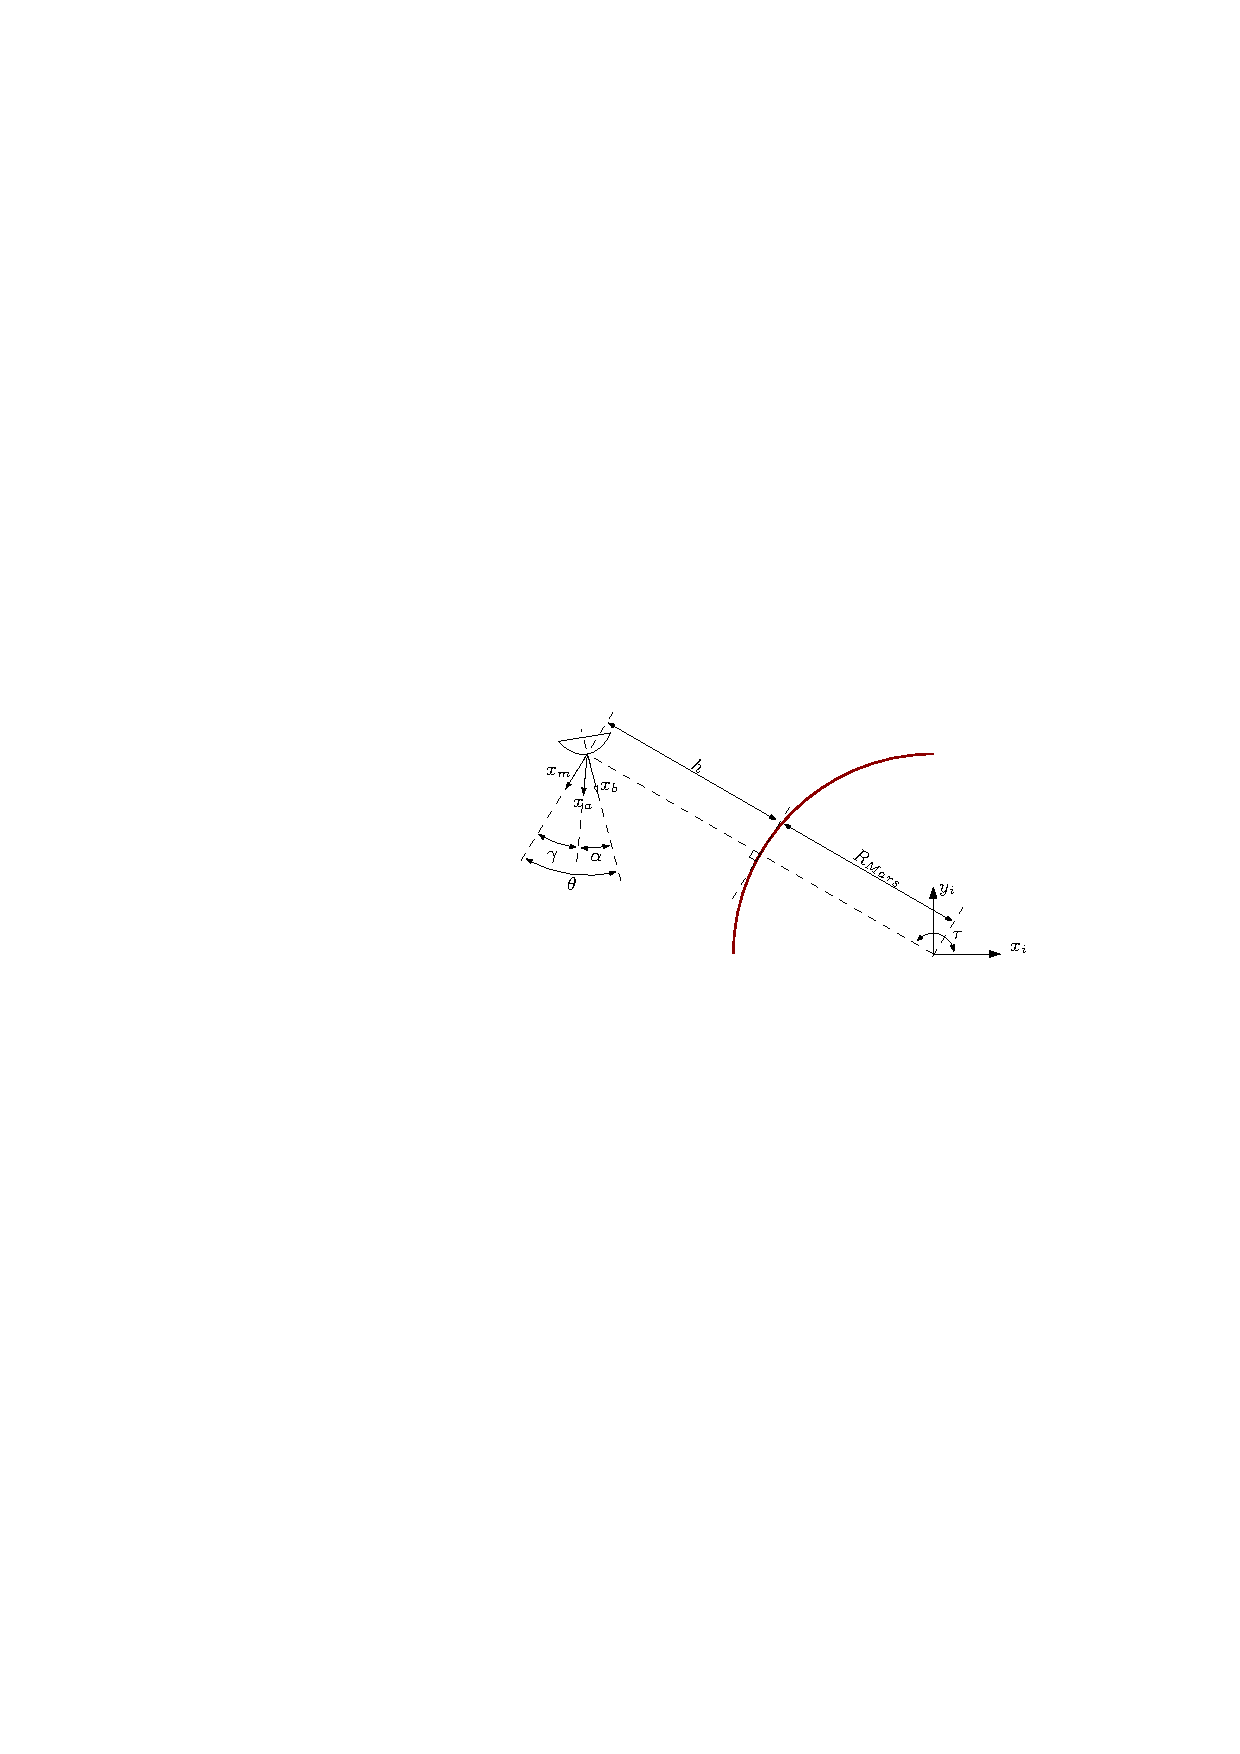
\includegraphics[width=0.7\textwidth]{Figure/Orbit/angles.pdf}
	\caption{The angles used in the simulation of the trajectory}
	\label{fig:angles}
\end{figure}

\subsubsection{Entry and descent}\label{sec:entry_descent}
The boost given in the apoareion before entry is determined such that the initial flight path angle ($\gamma$ as in Figure \ref{fig:angles}) of the entry is $17.2 \left[deg\right]$. Corresponding to this flight path angle an entry location (defined by $\tau$ in Figure \ref{fig:angles}) is dictated by the exit location of the aerocapture. With this location, flight path angle and the control as shown in Figure \ref{fig:orbit_entry_data}, the entry trajectory and final position are attained as shown in Figure \ref{fig:entry_mars}.

The objective of the entry and descent phase is to get to a height of $15 \left[km\right]$ with a velocity of $M = 5$ while keeping the deceleration under $3 \gls{sym:g}_{earth}$.

In order to keep the deceleration low, especially at the end of the descent, a low drag coefficient is required. This objective clearly conflicts with the properties needed for the aerocapture. As can be seen in Figure \ref{fig:orbit_entry_data} the deceleration at the end of the mission is right at the $3 \gls{sym:g}_{earth}$ limit for the nominal trajectory. Meaning the drag coefficient could not have gotten any higher.

In the last part of the descent also a high dynamic pressure is attained, which is the parameter that is the main input for inflatable structure design. The highest dynamic pressure is reached by the trajectory with a $10\%$ lower density.

In Figure \ref{fig:entry_mars} next to the nominal trajectory also two trajectories with a $10\%$ higher or lower density are plotted. The trajectory in the higher density atmosphere would land at a location before the nominal landing location if no change to the control is done. The trajectory that is shown for $10\%$ higher density is one with control that allows the vehicle to fly further (increased \gls{sym:mu}). This control causes the vehicle to overshoot the nominal landing location. Any point between these two margins is a possible landing location. It is thus proven that the nominal landing location can be achieved with $10\%$ higher density.

The trajectory for a $10\%$ lower density would normally overshoot the nominal landing location. The control is thus changed in order to push it towards the surface faster (lower \gls{sym:mu}). This control causes the vehicle to land before the nominal landing location. Again any point between these two margins is a possible landing location. This proves that the nominal landing location can be attained with $10\%$ lower density.

In Figure \ref{fig:entry_mars} it can also be seen that the entry locations for each trajectory is different. This flows down from the aerocapture where the exit location for these trajectories where different as well.

The time passed during both the aerocapture and the entry and descent phases are also different for each trajectory. During this time the landing location has rotated with Mars in the same direction as the flight direction of the vehicle. Three points for the nominal landing location can be distinguished in Figure \ref{fig:entry_mars}. Each point for the time one of the trajectories would arrive.

\begin{figure}[h]
	\centering
	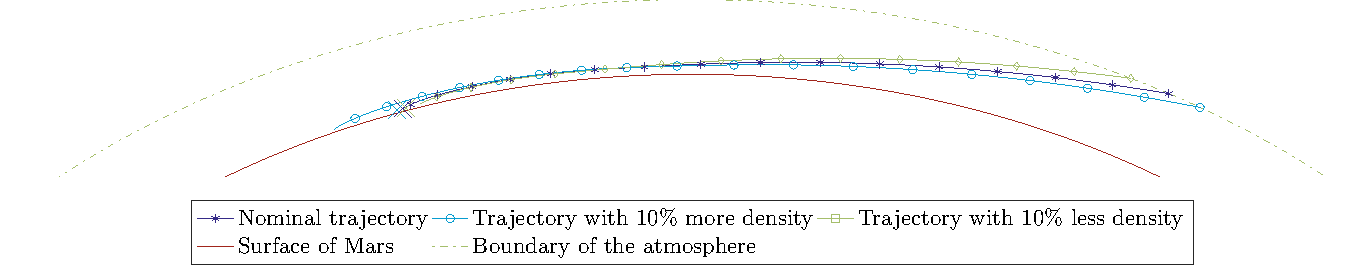
\includegraphics[width=0.99\textwidth]{Figure/Orbit/entry_mars.pdf}
	\caption[The re-entry trajectory for three different density profiles]{The re-entry trajectory for three different density profiles. The trajectories with modified density are corrected (changed \gls{sym:mu} profile) to show the ability to reach the desired landing location.}
	\label{fig:entry_mars}
\end{figure}

In Figure \ref{fig:orbit_entry_data} it can be seen that the Mach number at a height of $15 \left[km\right]$ is approximately $5$ for all orbits. The entry trajectory with a lower density is the shortest, however it also decelerates fastest overshooting the $3 \gls{sym:g}_{earth}$ requirement by 23\%. This higher deceleration is needed to reach the required velocity of $M=5$.

The entry trajectory with a higher density is the longest. The deceleration is also faster than for the nominal trajectory and it also overshoots the $3 \gls{sym:g}_{earth}$ requirement by $11\%$. This higher deceleration is caused by the denser atmosphere at a height of $15 \left[km\right]$.

\begin{sidewaysfigure}
	\centering
	\includegraphics[width=0.99\textwidth]{Figure/Orbit/sensitivity_entry.pdf}
	\caption[Results of the re-entry trajectory for three different density profiles]{Results of the re-entry trajectory for three different density profiles. The trajectories with modified density are corrected (changed \gls{sym:mu} profile) to show the ability to reach the desired landing location. The horizontal dashed lines are design limits (for the \gls{sym:M} and \gls{sym:acc} plots)}
	\label{fig:orbit_entry_data}
\end{sidewaysfigure}

\subsubsection{Required properties for aerodynamic shape design} \label{sec:trajectory_summary}
The required aerodynamic properties for the different phases of the mission are conflicting. For the aerocapture phase a high drag coefficient as well as a high lift coefficient is needed. For the entry phase still a high lift coefficient is needed, however also a low drag coefficient is required.

Compromising between these requirements an angle of attack has been chosen at which the $\gls{sym:L}\cdot\gls{sym:D}^{-1}$ is maximal in order to maximise the lift for certain drag. The aerodynamic shape should be designed in such a way that the drag at maximum $\gls{sym:L}\cdot\gls{sym:D}^{-1}$ is a perfect compromise between the objectives for the aerocapture and entry \& descent phases.


\subsection{Subsystem design} \label{sec:subsystemdesign}
%\subsubsection{Iteration process}\label{subsec:itproc}
%In order to structure the design process, several design aspects were separated to facilitate  iterating over the design. The goal is to find a design that complies with the requirements as given in Section \ref{sec:reqbreak}. This is done by choosing a design concept containing a combination of an aerodynamic shape, trajectory, \gls{tps}, inflation structure and control system and analysing its performance. After that, the analysis of the concept is used to assess possible points of improvement if the requirements are not yet met. This is repeated until all requirements are complied with. The design process is started with an initial design which is assessed for its performance which is then used as a baseline.

The aerodynamic shape is chosen such that certain aerodynamic properties are achieved. This is largely done by optimisation since this allows a high fidelity in design optimisation objectives and constraints. These aerodynamic properties are chosen based on the previous design analysis. 
When a suitable design is chosen, the resulting aerodynamic characteristics are used in determining a trajectory that complies with the initial and final velocity and height requirements. This is done by choosing a bank angle profile, choosing the bank angle as a function of time to arrive at the required location and velocity. 
The trajectory data containing velocity, density, Mach number and dynamic pressure is used for the inflation structure sizing, \gls{tps} lay-up and control system mass estimation. The shape and maximum dynamic pressure in the trajectory is used in determining the inflation structure, for which a parametric mass model is used to estimate the decelerator mass. 
Also, a representative truss structure is used to determine whether the loads don't exceed the material maximum loads. The heat flux into the system, which in turn amounts to a temperature distribution through the structure and through time, is calculated with the trajectory data. Numerically integrating the 1D heat equation with as input the heat flux data yields a temperature distribution for a given lay-up. The lay-up is then iterated until no layer temperature exceeds its maximum temperature while having the smallest thickness possible such that the \gls{tps} has the lowest possible mass. 
The control system mass is finally estimated using the required bank angle through the trajectory and moments of inertia.

When the technical analysis of the concept is done, the iteration is completed by analysing the results and assessing points where improvement can be made. When not all requirements are met, changes have to be made tot he design. Several problems have been identified during the design phase:
\begin{itemize}
	\item In the case the temperature in the different \gls{tps} layers become too high, even for high thicknesses, the orbit needs to be changed to facilitate a lower maximum dynamic pressure. This can be done by choosing the lowest point of atmospheric entry higher such that the density is lower. If achieving orbit at this higher point is not possible with the current aerodynamic design, the drag coefficient is to be increased to allow the same deceleration at lower dynamic pressures.
	
	\item If the thermal protection system mass or inflation structure mass makes the total design exceed the mass requirement, also the maximum dynamic pressure is to be decreased such that physical loads on the structure and thermal loads on the \gls{tps} are decreased.
	
	\item If bank angle control does not perform well enough to allow a trajectory that satisfies the requirements, the lift over drag ratio can be increased to allow more freedom in trajectory choice.
	
	
\end{itemize}

The iteration strategy is visualised as a flow-chart in Figure \ref{fig:iterativedesignflowchart}. In this figure the solid lines represent design information flowing towards the areas that still need analysis. In the `Design within requirements?' decision box, the check is made whether the mass is within budget and the temperature does not exceed the maximum temperature of the material. If this is the case, the design meets the requirements and is thus the acceptable choice.




\begin{figure}[h!]
		\vspace{-1cm}
		\includegraphics[width=0.8\textwidth]{./Figure/DesignIterationPhilosophy_new.pdf}
		
		\caption{The iterative design process flowchart}
		\label{fig:iterativedesignflowchart}
\end{figure}
This section will present the final designs of the \gls{hiad} subsystem. First Sections \ref{subsec:infldes}, \ref{subsec:depldes} and \ref{subsec:inflsys} will discuss the inflatable structure, deployment mechanism and inflation system respectively. Secondly Section \ref{subsec:controlsys} will mention the final control system design. Lastly Section \ref{subsec:crewmod} will give an overview of the crew module design.
\subsubsection{Inflatable structure}\label{subsec:infldes}
The inflatable structure consists of three main design elements: The aerodynamic shape, structural arrangement and \gls{tps} design. These elements will be covered in the subsequent sections in the aforementioned order.

\paragraph{Aerodynamic shape}
The aeroshell will have a shape similar to configuration D in Figure \ref{fig:aeroshapes} in Section \ref{subsec:aerosens}, with a radius of $6$ $\left[m\right]$ and a half cone angle of approximately $\gls{sym:theta_cone} = 70$ $\left[deg\right]$. The curved nose will have an outer radius of $2.5$ $\left[m\right]$. The cross-sectional offset at the rear of the body is approximately $0.91$ $\left[m\right]$. At an angle of attack of $\gls{sym:alpha} = 22.5$ $\left[deg\right]$, it has a lift-to-drag ratio of $\gls{sym:L} \cdot \gls{sym:D}^{-1} = 0.35\left[-\right]$ and a drag coefficient of $\gls{sym:CD} = 1.3$ $\left[-\right]$. At this angle of attack, a \gls{cg}-offset of $\gls{sym:CM}\cdot \gls{sym:lref} \cdot \gls{sym:CX}^{-1} = 0.5$ $\left[m\right]$ is required to trim the vehicle around the pitch axis. It has a moment derivative of $\gls{sym:cm-alpha} = -0.21$ $\left[rad^{-1}\right]$. 

 Figures \ref{fig:aeroshape.frontview} through \ref{fig:aeroshape.isoview} show the final \gls{oml} of the aeroshell. The final shape is composed of circular cross-sections stacked on top of each other, with an offset in the $z$-direction. The aeroshell is $1.8$ $\left[m\right]$ high and has a maximum offset of $0.9$ $\left[m\right]$.
 
\begin{figure}[h]
	\centering
	
	\begin{subfigure}[b]{0.49\textwidth}
		\includegraphics[width=0.99\textwidth]{./Figure/Aerodynamics/frontview.pdf}
		\caption{Front view}
		\label{fig:aeroshape.frontview}
	\end{subfigure}
	\begin{subfigure}[b]{0.49\textwidth}
		\includegraphics[width=0.99\textwidth]{./Figure/Aerodynamics/sideview.pdf}
		\caption{Side view}
		\label{fig:aeroshape.sideview}
	\end{subfigure}
	\begin{subfigure}[b]{0.49\textwidth}
		\includegraphics[width=0.99\textwidth]{./Figure/Aerodynamics/topview.pdf}
		\caption{Top view}
		\label{fig:aeroshape.topview}
	\end{subfigure}
	\begin{subfigure}[b]{0.49\textwidth}
		\includegraphics[width=0.99\textwidth]{./Figure/Aerodynamics/geometry_cp.eps}
		\caption{3D view}
		\label{fig:aeroshape.isoview}
	\end{subfigure}
	\caption{Front, side, top and 3D view of the inflatable shape}
\end{figure}
 
 Figures \ref{fig:CLCDCSAlpha} through \ref{fig:CGOAlpha} display the aerodynamic characteristics of the vehicle through an angle of attack range of $0 \left[deg\right]<\alpha<30 \left[deg\right]$. As can be seen from these plots, the behaviour of the lift-to-drag ratio and the moment coefficient in pitch is near linear. This linearity ensures predictable vehicle behaviour over the entire angle of attack range.
 
 \begin{figure}[h]
 	\centering
 	
 	\begin{subfigure}[b]{0.49\textwidth}
 		\includegraphics[width=0.99\textwidth]{./Figure/Aerodynamics/CDCSCLAlpha.pdf}
 		\caption{Force coefficients in the aerodynamic frame versus angle of attack}
 		\label{fig:CLCDCSAlpha}
 	\end{subfigure}
 	\begin{subfigure}[b]{0.49\textwidth}
 		\includegraphics[width=0.99\textwidth]{./Figure/Aerodynamics/CMXCMYCMZAlpha.pdf}
 		\caption{Moment coefficients in the body frame versus angle of attack}
 		\label{fig:CMxCMyCMzAlpha}
 	\end{subfigure}
 	\begin{subfigure}[b]{0.49\textwidth}
 		\includegraphics[width=0.99\textwidth]{./Figure/Aerodynamics/CLCDAlpha.pdf}
 		\caption{Lift-to-drag ratio versus angle of attack}
 		\label{fig:CLCDAlpha}
 	\end{subfigure}
 	\begin{subfigure}[b]{0.49\textwidth}
 		\includegraphics[width=0.99\textwidth]{./Figure/Aerodynamics/CGoAlpha.pdf}
 		\caption{Required \gls{cg}-offset versus angle of attack}
 		\label{fig:CGOAlpha}
 	\end{subfigure}
 	\caption{Various aerodynamic characteristics of the aeroshell over the angle of attack range $0<\alpha<30$ [$deg$]}
 \end{figure}


\paragraph{Structural analysis and design}


The inflatable consists of ten toroids, stacked aside and on top of one another. The asymmetric shape obtained by aerodynamic optimisation is attained by arranging the toroids at an angle with respect to one another. The result is an assembly of circular inflatables, placed at differing radial distances with respect to the centre body. While the structural performance of the inflatable is altered, an asymmetric configuration is achieved by stitching the toroids and varying the radial length of the straps over the sphere cone circumference. Structural performance is altered in the sense that the asymmetry of the configuration implies additional concerns for aero-elastic phenomena, such as limit cycle oscillations, for example. These phenomena, however, are highly unpredictable and warrant additional wind tunnel and flight testing in any case. 

The number of toroids is based on Figure \ref{fig:inflpress_strucmass}, which shows that mass decreases beyond ten toroids are insignificant. Moreover, ten toroids are sufficient to adequately represent the optimised aerodynamic shape. 

Structural loads are carried by PBO Zylon\textsuperscript{\textregistered} fibres, interlaced warp and weft to provide load-carrying capability in all required directions: circumferential and hoop. As such,fibres are woven perpendicular to each other. To this end, a plain weave pattern is adequate.

For the load analysis, the ultimate load is calculated by multiplying the limit load, a peak dynamic pressure of 2300 [$Pa$] (with a $10\%$ density deviation from the nominal density), with a \acrfull{fos} of 1.5. This \gls{fos} respects NASA standards for composite structures and accounts for uncertainties in the maximum external loading applied \cite{Technical2014}.  
From Figure \ref{fig:mat} and the parametric mass model it follows that for this ultimate load Vectran and aramid fibres Kevlar and Technora have exceeded their minimum gage thickness, set at 0.125 [$mm$] for aramid fibres. 

Such a minimum thickness is achievable for a plain weave, based on its proposed application in \gls{irve}-4 in a 0.127 [$mm$] lay-up \cite{Litton2011} and commercial availability of these weave patterns for Kevlar\footnote{URL: \url{http://www.cstsales.com/aramid_fabric.html}. Accessed: 16-06-2015}. Based on available grades of Vectran\footnote{URL: \url{http://www.swicofil.com/vectran.html\#Grades}. Accessed: 17-06-2015}, its minimum thickness is set at 0.023 [$mm$]. PBO Zylon\textsuperscript{\textregistered}, on the other hand, remains at its minimum gage thickness for this loading. This minimum thickness is assumed to be the same as that of Kevlar, an assumption supported by the same yarn count and sample thickness in a study on ballistic impact on Kevlar 49 and PBO Zylon\textsuperscript{\textregistered} \cite{Pereira2009}. 

PBO Zylon\textsuperscript{\textregistered} offers a mass advantage of approximately 5 [$kg$] with respect to Technora and Vectran and 10 [$kg$] with respect to Kevlar. This mass advantage is the first reason for opting for PBO Zylon\textsuperscript{\textregistered}. In addition, PBO Zylon\textsuperscript{\textregistered} is capable of withstanding higher temperatures, 400 $\left[^{\circ}C\right]$ for short exposure versus 250 $\left[^{\circ}C\right]$ for Kevlar 49, one of the key drivers for its implementation in the upcoming \gls{thor} mission \cite{Dillman2014}. While in principle this would allow for a lighter \gls{tps}, this advantage is included as an additional contingency. At this stage, PBO Zylon\textsuperscript{\textregistered} fibres have not been applied in \gls{hiad} missions, in contrast to Kevlar 49 fibres. Since the mass limit is not exceeded, the mass advantage is not required and reliability is preferred due to the criticality of the inflatable. 

%Key driver for the design case at hand is the minimum material thickness: the loading was thusly low that the required thickness to withstand loads induced by aerodynamic and inflation pressure is lower than minimum gage thicknesses. To this end, fibre weight performance is mainly dictated by density and minimum gage thickness. The flexible material mass achieved by Spectra 2000, expected to perform best of all fibres given its low density of 970 [$kg \cdot m^{-3}$], compared to Kevlar's 1440 [$kg \cdot m^{-3}$], is 20 [$kg$] lower than that achieved by Kevlar 49 and the other fibres, of comparable density. 

%Preference is given to Kevlar 49, however, for two reasons. Firstly, it is widely commercially available and has been applied for a longer number of years, with resulting lower costs associated with its fabrication and application. Secondly, it has been previously applied for inflatable re-entry vehicles, namely in the \gls{irve} missions \cite{Hughes2011}. Spectra 2000 therefore introduces additional costs and technical risks that offset the weight advantage offered. Moreover, the weight advantage does not further the entry vehicle in the sense that supplementing another crew member is out of reach and requirements are respected. Other fibres are comparable to Kevlar in their performance, with none of the benefits of past application in \glspl{hiad}.

%Based on the parametric mass model and the inherent stress equations, the minimum gage thickness of 0.125 [$mm$] is deemed attainable. Such a minimum thickness is achievable for a plain weave, based on its proposed application in \gls{irve}-4 in a 0.127 [$mm$] lay-up \cite{Litton2011} and commercial availability of these weave patterns\footnote{URL:\url{http://www.cstsales.com/aramid_fabric.html}. Accessed: 16-06-2015}. 

The structural feasibility of the configuration is ascertained by the truss-based analysis model. The truss-based analysis model uses the representation in Figure \ref{fig:strucreps}. Cross-sections that displayed the most extreme loading are the short side, defined at the inflatable minimum diameter, and the long side, defined at the inflatable maximum diameter. Due to the skewness, load asymmetry is introduced which is thereby evaluated by some extent through evaluation of multiple cross-sections.

\begin{figure}[h]
	\centering

	\begin{subfigure}[b]{0.45\textwidth}
		\includegraphics[width=0.96\textwidth]{./Figure/Structure/shape_long.eps}
		\caption{Cross-sectional view at maximum diameter}
		\label{fig:shapel}
	\end{subfigure}
	\begin{subfigure}[b]{0.45\textwidth}
		\includegraphics[width=0.96\textwidth]{./Figure/Structure/shape_short.eps}
		\caption{Cross-sectional view at minimum diameter}
		\label{fig:shapes}
	\end{subfigure}
\begin{subfigure}[c]{0.5\textwidth}
		\includegraphics[width=0.96\textwidth]{./Figure/Structure/struc_rep.eps}
		\caption{Isometric view}
		\label{fig:iso}
	\end{subfigure}
\caption{Structural representation of inflatable structure}
\label{fig:strucreps}
\end{figure}

For an inflation pressure of 169 [$kPa$], required to bring all members into tension, structural loads are as obtained in Figures \ref{fig:strucl} and \ref{fig:strucs}. It can be observed that the maximum running load in the walls is 50 [$kN \cdot m^{-1}$]. Translating this to a stress by dividing through the 0.125 [$mm$] thickness yields a maximum stress of 400 [$MPa$], well below the (room-temperature) tensile strength of 5.8 [$GPa$] for PBO Zylon\textsuperscript{\textregistered}. In the straps, the maximum running load is 100 [$kN \cdot m^{-1}$], translating to a 800 [$MPa$] stress. As such, the minimum gage thickness is well above the required thickness determined by preliminary load and stress analysis. Firstly this takes into account material strength loss at higher temperatures, as PBO Zylon\textsuperscript{\textregistered} retains $80\%$ of its strength when exposed to 200 $\left[^{\circ}C\right]$. Secondly, it takes into account a wide margin for material uncertainties, production deficiencies and unpredicted structural phenomena. The flexible material mass, given a uniform thickness of 0.125 [$mm$] for radial straps and toroid material, is 110 [$kg$].

\begin{figure}[h]
		\hspace{-16mm}
		\includegraphics[width=1.2\textwidth]{./Figure/Structure/loads_long.eps}
		\caption{Cross-sectional running loads inflatable at maximum diameter}
		\label{fig:strucl}
\end{figure}
\begin{figure}[h]
		\hspace{-16mm}
		\includegraphics[width=1.2\textwidth]{./Figure/Structure/loads_short.eps}
		\caption{Cross-sectional running loads inflatable at minimum diameter}
		\label{fig:strucs}
\end{figure}

Stitching of the fabrics making up the toroids is used for the joints of the inflatable, on one hand to join the toroids to each other and on the other hand to join the toroids to the radial straps. This is a method excellently suited, applied, tested and proven in the \gls{irve} missions \cite{Lindell2006,Hughes2011,Dillman2012}. Joints are thereby proven high-strength and suitable for space application and a stacked-toroid configuration.

To prevent the inflation gas from leaking, the structural PBO Zylon\textsuperscript{\textregistered} layers are coated with a gas barrier in the form of a 50 [$\mu m$] Upilex layer. This uniform thickness coating adds an estimated 25 [$kg$]. The thickness of this coating is feasible, in line with findings by Samareh and Miller \cite{Samareh2011,Miller2014} and available Upilex grades of 12.5, 25, 50, 75 and 125 [$\mu m$]\footnote{URL: \url{https://www.ube.com/content.php?pageid=81}. Accessed: 16-06-2015}$^{,}$\footnote{URL: \url{http://dasp.mem.odu.edu:8080/~deorbit_sp12/ref/UPILEXS\%20Data\%20sheet.pdf}. Accessed: 16-06-2015}.

%Typical driver for the use of fibres are the high mechanical properties, hence the application of Kevlar in the \gls{irve} missions \cite{Hughes2011}. Structural analyses proved the weight advantage of fibres over films in the case of \gls{irve}. In this case, however, density is leading and the mechanical properties of fibres are excessively high: their application would lead to an overdesign. This is reflected by Table \ref{tab:matfinal}. The flexible material mass achieved by Spectra 2000, expected to perform best of all fibres given its low density of 970 [$kg \cdot m^{-3}$], compared to Kevlar's 1440 [$kg \cdot m^{-3}$], is 20 [$kg$] lower than that achieved by Kevlar 49. 

%Films, however, provide a significant weight advantage. Upilex-25S and Kapton are films suitable for \gls{hiad} application \cite[p.59]{Balasooriyan2015b}. Upilex-25S is characterized by higher mechanical properties than Kapton, and due to the low minimum thickness for these films specific strength is the leading material property. The specific strength of Upilex-25S is nearly twice as high as that of Kapton \cite{Samareh2011} and this is reflected by its mass, nearly twice as low. The predominant advantage of using Upilex-25S over fibres is therefore directly reflected by the lower achievable structural mass, yielding a flexible material mass of 30 [$kg$].
%\begin{table}[h]
%\centering
%\caption{Comparison of flexible material mass for use of different materials}
%\label{tab:matfinal}
%\begin{tabular}{|l|l|l|l|l|}
%\hline
%{\bf Material}                        & Kevlar 49    & Spectra 2000 & Upilex-25S & Kapton \\ \hline
%{\bf Type}                            & Aramid fibre & Aramid fibre & Film       & Film   \\ \hline
%{\bf Flexible material mass {[}kg{]}} & 89             &  71          &  31          & 52        \\ \hline
%\end{tabular}
%\end{table}

%The weight advantage is predominantly effected by a lower minimum gage thickness for films. Minimum gage thickness for Upilex-25S is 25 [$\mu m$]\footnote{URL:\url{http://dasp.mem.odu.edu:8080/~deorbit_sp12/ref/UPILEXS\%20Data\%20sheet.pdf}. Accessed: 16-06-2015}.  The thickness required to withstand the loads is estimated at 0.025 [$mm$]



%As such, based on the discussion in Subsection \ref{subsec:strucsens} Spectra 2000 is expected to perform best given its low density of 970 [$kg \cdot m^{-3}$], compared to Kevlar's 1440 [$kg \cdot m^{-3}$]. This effects a 20 [$kg$] decrease in material mass by the use of Spectra 2000 as compared to the other materials in Figure \ref{fig:mat}, of comparable density with Kevlar 49. 

%Stitching of the fabrics making up the toroids is used for the joints of the inflatable, on one hand to join the toroids to each other and on the other hand to join the toroids to the radial straps. This is a method excellently suited, applied, tested and proven in the \gls{irve} missions \cite{Lindell2006,Hughes2011,Dillman2012}. Joints are thereby proven high-strength and suitable for space application and a stacked-toroid configuration.

%Structural integrity is provided by PBO Zylon AS, capable of retaining its strength at high temperature and able to withstand the required loads\footnote{URL:\url{http://www.toyobo-global.com/seihin/kc/pbo/zylon-p/bussei-p/technical.pdf}. Accessed: 15-06-2015}}. It has high specific properties, leading to a low structural mass, as follows from Figure \ref{fig:mat}. It performs only slightly worse than Spectra 2000 in the parametric mass model, but differences are slight (below 5 $\%$) and 

\clearpage

\paragraph{\acrlong{tps} design}
For a given trajectory and lay-up it is possible to check the temperature distribution for failure. From the sensitivity analysis in Section \ref{subsec:thermalsens} it is deducted that a Nextel BF-20 layer with Pyrogel\textsuperscript{\textregistered} 6650 as insulator is preferable for mass reduction purposes. However, due to the relatively low emissivity of Nextel the wall temperature exceeds the limit as high aerodynamic heating can not be radiated away efficiently. For this reason a slightly heavier alternative, Nicalon\textsuperscript{TM}, is needed. Nicalon\textsuperscript{TM} is a type of silicon continuous fibre that can withstand temperatures up to 2073 $\left[K\right]$. Furthermore it has a much higher emissivity, which greatly reduces the wall temperature. It performs comparable or even better on its ability fold compared with Nextel BF-20 \cite{Corso2011}. The sensitivity analysis has shown that for a diameter of 12 $\left[m\right]$ it was not possible to find a viable thickness for the Nextel lay-ups. Several iterations have been performed to reduce the heat flux such that Nextel BF-20 became viable, however these attempts resulted only in an approximate mass of 500 $\left[kg\right]$. Therefore Nicalon\textsuperscript{TM} is chosen as \gls{tps}-layer and Pyrogel\textsuperscript{\textregistered} 6650 as insulation layer for the lay-up in the final design. In addition to the Upilex coating on the inside of the PBO Zylon\textsuperscript{\textregistered} layer, two thin impermeable layers of kapton are placed between the Pyrogel\textsuperscript{\textregistered} and Zylon\textsuperscript{\textregistered} to prevent hot gasses reaching the Zylon\textsuperscript{\textregistered} layer \cite{Hughes2005,Litton2011}.

The incoming heat flux, or aerodynamic heating of the chosen trajectory is shown in Figure \ref{fig:heatfluxes}. The heat maximum heat flux is approximately 21 $\left[W\cdot cm^{-2}\right]$. The maximum heat flux for the entry phase is 7.3 $\left[W\cdot cm^{-2}\right]$. It is expected that this entry phase is not leading for the design and therefore it is not shown. In the figure three fluxes are shown for the aerocapture phase, which represent the change in heat flux when the atmospheric density is over- or underestimated by $10\%$. This $10\%$ comes from the uncertainties in the density as explained in Section \ref{sec:trajectorydesign}. Surprisingly, when the density is underestimated by $10\%$, the heat load becomes slightly higher as the duration of the trajectory is longer and this results in a higher required thickness. This case is used as reference heat flux for which the lay-up is optimised.

\begin{figure}[h]
	\centering
	\includegraphics{./Figure/Thermal/heatfluxes.pdf}
	\caption{Heat flux of the aerocapture for different density levels}
	\label{fig:heatfluxes}
\end{figure}

Figures \ref{fig:thermoaero} and \ref{fig:thermoentry} show how the heat propagates though the material during the aerocapture and entry phase of the chosen trajectory. It is clear that the aerocapture is indeed leading for the design as the heat load during this phase and resulting temperatures are higher. The figure can also be used to understand the required thicknesses. The Nicalon\textsuperscript{TM} and Pyrogel\textsuperscript{\textregistered} layers remain far below their maximum temperatures, 2073 $\left[K\right]$ and 923 $\left[K\right]$ respectively. Therefore the Nicalon\textsuperscript{TM} layer is as thin as possible, which is 0.508 $\left[mm\right]$. For the kapton and PBO Zylon\textsuperscript{\textregistered} layers the maximum temperature is set at 473 $\left[K\right]$ to remain their structural integrity. This is why the insulation layer is needed such that the temperature drops to this maximum through the Pyrogel\textsuperscript{\textregistered} 6650. The required thickness for this is 2.439 $\left[mm\right]$. Each kapton layer is also very thin which comes down to 0.025 $\left[mm\right]$.

\begin{figure}[h]
	\centering
	\begin{subfigure}[b]{0.45\textwidth}
		\includegraphics[width=\textwidth]{./Figure/Thermal/Thermal_contour_capture.eps}
		\caption{Aerocapture}
		\label{fig:thermoaero}
	\end{subfigure}
	~ %add desired spacing between images, e. g. ~, \quad, \qquad, \hfill etc.
	%(or a blank line to force the subfigure onto a new line)
	\begin{subfigure}[b]{0.45\textwidth}
		\includegraphics[width=\textwidth]{./Figure/Thermal/Thermal_contour_entry.eps}
		\caption{Entry}
		\label{fig:thermoentry}
	\end{subfigure}
	\caption{Heat propagation during both decelerations}\label{fig:heatprop}
\end{figure}

The areal density of this lay-up is 1.816 $\left[kg\cdot m^{-2}\right]$. The frontal surface area or wetted area is 120.9 $\left[m^2\right]$, as is obtained from the aerodynamic analysis. Multiplying the surface area with the area density results in a frontal \gls{tps} mass of 219.6 $\left[kg\right]$. Note that the frontal \gls{tps} covers the rigid centre body of the vehicle. For the protection on the other side of the inflatable very thin layers of kapton and Nextel AF-14 are assumed to be sufficient. The resulting area density is 0.342 $\left[kg\cdot m^{-2}\right]$. The area onto which it is applied is assumed to be the frontal surface area minus the centre body area, which equals to 105.0 $\left[m^2\right]$. The resulting mass is 35.96 $\left[kg\right]$. The total \gls{tps} mass for the lay-up shown in Figure \ref{fig:finallayup} yields 255.6 $\left[kg\right]$. 

\begin{figure}[H]
	\centering
	\includegraphics{./Figure/Thermal/finallayup.pdf}
	\caption{Final design for the \acrlong{tps}}
	\label{fig:finallayup}
\end{figure}


%\subsubsection{Centerbody connector}\label{subsec:centerbodydes}
%\input{./Chapter/Final_Design/Subsystem_design/Centerbody_design}

\subsubsection{Deployment mechanism}\label{subsec:depldes}
This subsection presents the design of the deployment mechanism to bring the inflatable from its stowed to its deployed configuration. It is key that this action is performed with maximum reliability, since deceleration of the entry vehicle and thereby mission success hinges on the aerodynamic surface area provided by the inflatable decelerator. This design comprises selection of a \acrfull{hdrm}, a canopy to protect the inflatable during interplanetary transfer and its detachment, and deployment.

Deployment of inflatables can be performed either by unrolling, unfolding or deploying a strut \cite[p.222-227]{Jenkins2001}. The former two are deemed impractical for the following reason. Unrolling and unfolding in lateral direction from the centerbody are less package efficient than deploying it as a strut. Unrolling requires a hub about which is rolled and results in multiple toroids stacked together laterally. Unfolding compresses the toroids and thereby also features multiple toroids in lateral direction. Deploying, on the other hand, stretches the sphere cone shape in axial direction and thereby features no more than one toroid in lateral direction. Unrolling and unfolding thus take up more space in radial direction through denser packing in this direction, while deploying stretches the packaging over the axial direction. A key driver for the use of inflatable aeroshells is the launch vehicle constraint on diameter in stowed configuration. By requiring less diameter for aeroshell package, more diameter is left free for the centerbody design. This results in maximum efficiency in the use of available diameter and thereby a more weight-efficient design, since an increase in centerbody diameter is deemed less weight-expensive than an increase in inflatable diameter for a given deployed diameter. This is a result supported by the sensitivity analysis presented in section \ref{sec:strucsens}. 

\begin{figure}[h]
	\centering

	\begin{subfigure}[b]{0.49\textwidth}
		\includegraphics[width=0.96\textwidth]{./Figure/Structure/rot.png}
		\caption{Rotational deployment mechanism}
		\label{fig:rot}
	\end{subfigure}
	\begin{subfigure}[b]{0.49\textwidth}
		\includegraphics[width=0.96\textwidth]{./Figure/Structure/fold.png}
		\caption{Folding deployment mechanism}
		\label{fig:fold}
	\end{subfigure}
		\begin{subfigure}[b]{1\textwidth}
		\centering
			\includegraphics[width=0.3\textwidth]{./Figure/Structure/hinge.png}
			\caption{Hinging deployment mechanism}
			\label{fig:hinge}
		\end{subfigure}
	\caption{Overview of various deployment possibilities \cite{Jenkins2001}}
	\label{fig:dep}
\end{figure}


Moreover, less interference between flexible material is present when deploying the inflatable sphere cone, as opposed to the folding and rolling of the toroids in the other two methods. This decreased amount of interference reduces the unpredictability and thereby increases reliability of the deployment procedure.

Deploying does attachment points at which the outer toroid is held in place in stowed configuration. The axial length over which the inflatable is held in stowed condition is equal to the inflated radius minus the centerbody radius, equal to XXX [m]. Attachment points will therefore be located at the side of the crew module, such that the inflatable is wrapped about the vehicle in stowed condition. 

To initiate deployment events \glspl{hdrm} are used. As deployment is a singular event in time, one-time use is warranted. Reusable mechanisms typically have a larger number of moving parts and thereby a lower reliability than non-reusable mechanisms \footnote{URL: \url{http://www.esa.int/Our_Activities/Space_Engineering_Technology/Mechanisms/Hold-Down_and_Separation_Systems}. Accessed: 04-06-2015}. Reliability is key, since deployment of the aeroshell is of singular importance to aerodynamically decelerate the vehicle. To this end, pyro cutters are the pre-eminent solution by their high and proven reliability in space operations, low weight and shock imparted to the vehicle. Example cutters are Chemring Hi-Shear cutters, applied in multiple space missions, such as the Mars observer mission \footnote{URL: \url{http://www.hstc.com/Products/OrdnanceProducts/CuttersBoltRodandCab/}. Accessed: 08-06-2015}. These possess a weight in the order of one hundred grammes. For their criticality in mission success, redundancy of \glspl{hdrm} is key and at each location at least two cutters are required to be present.



\subsubsection{Inflation system}\label{subsec:inflsys}
The inflation gas is key to providing the structural stiffness for the inflatable: it is required to bring all members into tension to prevent skin wrinkling under compressive loading. To this end, the aeroshell will require an inflation system that is reliable, lightweight and fitting within mass and volume constraints. This subsection details the selection of an inflation gas and design of the inflation system upon which aeroshell deceleration capability hinges.

\paragraph{Gas generator selection}
Inflation systems can be categorised as tanked-gas systems, phase-change systems and chemical gas-generation systems \cite{Jenkins2001}. These systems have each been considered for their respective advantages, yielding a tanked nitrogen inflation system as outcome. 

%\paragraph{Phase-change system}
Phase-change systems have the potential to provide significant mass reductions. The most promising option is a liquid hydrogen inflation system, while other phase-change systems involve subliming powders, although these are incapable of achieving high pressures \cite{Freeland1998}.  On the basis of system mass fractions investigated by Brown et al. \cite{Brown2009} and the mass estimation tool detailed in section \ref{subsec:structool}, a structural mass reduction of nearly 20 [$kg$] is deemed feasible with a cryogenic liquid hydrogen inflation system following from the mass estimation tool formulated in section \ref{subsec:structool}. 


This mass reduction comes at the expense of reliability, however. These systems involve a phase-change process, inherently unpredictable and thereby accompanied with reduced inflation system reliability \cite{Jenkins2001}. In addition, cryogenic storage requires profound thermal control to keep it below its required temperature. While this poses a challenge for orbiting satellites, it is even more so an issue in the heated re-entry environment of the inflatable aeroshell. Reliability is further lessened by the absence of successful efforts in the past to accommodate a phase-change inflation system in spaceflight, let alone a high-pressure application like the aeroshell at hand. As reliability is key for transporting human payload, phase-change systems are deemed ill-suited. Moreover, a liquid hydrogen inflation system poses issues for safety when operating in the Earth atmosphere, in which flammability risk is present by the dual presence of hydrogen and oxygen in a heated environment. Re-entry on Earth should be considered for possible return missions of the inflatable aeroshell.


%\paragraph{Chemical gas-generation system
Chemical gas-generation systems similarly feature a higher level of complexity and thereby lower level of reliability than tanked-gas systems \cite{Jenkins2001}. Moreover, while mass reductions are deemed feasible, these involve the use of hydrazine \cite{Jenkins2001, Freeland1998}. Hydrazine poses issues with respect to cost and handling, but most importantly with respect to sustainability. As the decelerator will make contact with a hard surface, leakage of hydrazine into the Martian atmosphere and pollution of the landing site by its toxic nature poses a risk. This risk would violate \gls{cospar} regulations and moreover limit the sustainable dimension of the mission.

Tanked-gas systems are the preferred choice, featuring a significantly higher level of reliability and past application. Most notably, these have seen application in the \gls{irve} missions in the form of a nitrogen blow-down system \cite{Smith2010}. Blow-down systems offer controllable gas flow at low development and hardware cost \cite{Freeland1998}. Moreover, these are excellently suited for high-pressure applications in inflatable structures \cite{Jenkins2001}.

Using helium rather than nitrogen would be infeasible. Due to the small size of helium atoms, permeability of the tank and inflatable becomes an issue and pressure leakage a more pronounced phenomenon. Moreover, helium application in spacecraft applications has remained uninvestigated in literature and thereby poses significantly higher development risk.


\paragraph{Gas generator design and sizing}
A nitrogen tank is used for storage and supply of nitrogen gas. The minimum inflation pressure in the toroids is based on the premise that it should counteract the aerodynamic force exerted to bring flexible material into tension, formulated in Equation \ref{eq:Pmin}. The volume that is inflated may be approximated as the sum of the volumes of separate toroids summated over the entire sphere cone.

From the structural analysis it followed that a pressure of 3.9 [$kPa$] over a total volume of 68 [$m^{3}$] is required in the inflatable bladders. This minimum inflation pressure is smaller than that required in \gls{irve}-3 \cite{Jurewicz2011}, hence it induces smaller loads, which make up most of the flexible wall loading and the structural lay-up can consequently be thinner than in the case of \gls{irve}-3. The inflation pressure brings all members into tension, as illustrated by Figures \ref{fig:strucl} and \ref{fig:strucs}.

To account for pressure losses following from a drop in temperature, as observed in the \gls{irve}-II mission \cite{Dillman2012}, a heater is used to heat the tank after partial usage of the inflation gas. The total mass of the inflation gas can be estimated on the basis of the required operating pressure. From a functional perspective the minimum required inflation pressure should be reached at all phases of the deceleration. Thermal loading of the aeroshell will increase the temperature of the inflation gas and cause a proportional increase in pressure. Pressure increases above the minimum inflation pressure are beneficial as this will increase the stiffness of the aeroshell. This works up to some point as structural loading has to be taken into account as well. If the pressure increases to much venting may be performed to reduce the pressure, which will be further discussed in the subsequent paragraph. Pressure decreases below the minimum required pressure are however dangerous as the stiffness of the aeroshell will be lost.

For this reason a minimum operational temperature is considered. Figure \ref{fig:tanktemp} shows the temperature range in Kelvin for a cylindrical body emitted by the sun from the side around Mars. The temperature is based on heat flow equilibrium, not considering any of the atmospheric entry effects \cite{Wertz2011}. A range of absorptivity over emissivity values is considered. This value is dependent on the outer coating of the spacecraft and is an large extend left free to be chosen. Nevertheless a conservative value of 0.5 is chosen which yields a temperature of 202 [$K$]. Lower temperature increases are not envisioned for a threefold of reasons:

\begin{itemize}
\item The Martian atmospheric temperature ranges between 100 and 200 [$K$], but conduction is low and only for the short period within the Martian atmosphere
\item Solar radiation will still heat the re-entry vehicle
\item Thermal loading will cause an increase in temperature even after the heat shield of the inflatable.
\end{itemize}

\begin{figure}[h]
		\centering
		\includegraphics[width=0.7\textwidth]{./Figure/Structure/Temp.pdf}
		\caption{Temperature range for a cylinder at Mars as function of the absorptivity over emissivity}
		\label{fig:tanktemp}
\end{figure}

Using a temperature of 202 $[K]$ inside the inflatable yields a total gas mass of 90 $[kg]$ that is to be held within the pressure tank, given a molar mass of 22 $[g\cdot mole^{-1}]$ for nitrogen gas \cite{Samareh2011}. An additional contingency of $20\%$ is included. This contingency accounts for leakage, which requires additional gas to make up for the lost volume, so called make up gas \cite{Jenkins2001}.

The ratio of tank and inflatable volume is obtained via the ideal gas law as:

\begin{equation}
\frac{\gls{sym:vol}_{tank}}{\gls{sym:vol}_{inflatable}} = \frac{P_{infl}T_{tank}}{P_{tank}T_{infl}}
\label{eq:volratio}
\end{equation}

Initial estimates for the tank pressure and temperature are 27.6 $[MPa]$ and 323 $[K]$ \cite[p.545]{Wertz2011}. Based on the required pressure and a temperature of 202 $[K]$ in the inflatable, by use of the ideal gas law, a total pressure tank volume of 0.27 $[m^{3}]$ follows. Corresponding to this tank volume is a required tank mass, dependent on the material used. Composite overwrapped pressure vessels offer significant weight advantages with respect to metallic tanks and therefore such a pressure vessel is selected. Tank mass is estimated from empirical relations established by Zakrwski \cite[p.546]{Wertz2011} to be 61 $[kg]$ for the selected tank pressure and volume via Equation \ref{eq:tmass}.
\begin{equation}
m_{tank} = 0.7266 \cdot (P_{tank} \cdot \gls{sym:vol}_{tank})^{2} + 2.5119 \cdot (P_{tank} \cdot \gls{sym:vol}_{tank}) + 2.9826
\label{eq:tmass}
\end{equation}

\paragraph{Inflation system integration}

Figure \ref{fig:infsys} shows a schematic representation of the inflation system. The inflation gas is stored in a nitrogen tank. Pressure and temperature sensors are included to monitor the storage conditions. A separate valve is included for filling purposes of the tank, and a release valve is included for emptying the tank outside normal mission operations. A electromechanical valve releases the pressure. A electromechanical valve is used since it allows for multiple uses as opposed to one-time use pyrotechnical valves, used in early \gls{irve} instalments \cite{Hughes2005}. From the high pressure within the storage tank the controlled the pressure is reduced and more precisely controlled by a set of two pressure regulators (including internal release valves). One of the pressure regulators is located in the high-pressure part of the inflation system in the centre body, the other in the low-pressure part. Duality of pressure regulators accounts for flow adjustment while also taking into account feed losses. A set of check valves, allowing flow only in one direction, connects to the toroid. Purpose thereof is to prevent flow from exiting the bladder volumes. 

The toroids are grouped together and inflated with separate bladder volumes.  The number of bladder volumes is preferably higher to provide redundancy. A single bladder volume puncture or failure would then be less catastrophic, as part of its function can be taken over by other bladders. Increasing the number of bladder volumes does, however, add additional system complexity and mass. The \gls{irve} missions feature three bladder volumes, taken as a reference number. The current mission features a significantly larger area, however, and since puncture probability is thereby increased due to the larger exposed surface area. To this end five inflatable bladder volumes are selected. The check valves prevent the flow from equilibrating over the toroids in this case.

A final set of check valves is included to connect the toroids to the vent. This allows for reducing the pressure in case it becomes to high. The conditions within the tank are measured by a set of pressure and temperature transducers. If the pressure becomes to high, for example due to the thermal heating, the vent functions to lower the pressure. Pressure transducer however are also important for making sure the minimum pressure is maintained since the pressure can drop due to leakage. 

\begin{figure}[h]
		\centering
		\includegraphics[width=0.95\textwidth]{./Figure/Structure/infsys.pdf}
		\caption[Schematic view of the inflation system]{Schematic view of the inflation system}% (adapted from \cite{Hughes2005})}
		\label{fig:infsys}
\end{figure}


A contingency of $25\%$ of tank mass is included to account for the blow-down system that transfers gas from the tank to the inflatable volumes. For a tank mass of 61 $[kg]$, total inflation system mass is 76 $[kg]$ to support a gas mass of 90 $[kg]$.

\subsubsection{Control system}\label{subsec:controlsys}
This section will discuss the control system selection procedure and control system design. First the control system downselect will be discussed, after which the resultant control system will be sized to the mission requirements.
\paragraph{Control system selection}
Based on the arguments for and against certain control system concepts given in Chapter \ref{subsec:controltool} a selection of suitable control system solutions was made. Figure \ref{fig:cgoffset} shows the \gls{cg} offset required along the Z-axis to trim the spacecraft at certain angles of attack for various \gls{cg} locations on the X-axis. 
\begin{figure}[h]
	\centering
	\includegraphics[width=0.95\textwidth]{./Figure/control/moment}
	\caption[\acrlong{cg} offset along Z-axis required for a trimmed condition at various angles of attack]{\gls{cg} offset along Z-axis required for a trimmed condition at various angles of attack}
	\label{fig:cgoffset}
\end{figure}
From Figure \ref{fig:cgoffset} it can be seen that the required \gls{cg} Z-offset grows as the X-offset grows. For an angle of attack change of $2$ degrees corresponding to an X-\gls{cg} located at $-5$ meters a \gls{cg} shift of $0.2$ $[m]$ is required. Angle of attack-based trajectory control was found to require trimmed \gls{sym:alpha}-shifts of $5$ degrees that have to be adjusted with a rate of $1$ $[deg \cdot s^{-1}]$. To pull this off would require the actuation system to produce a \gls{cg} displacement of $0.5$ meters with a required rate of $0.1$ $[m \cdot s^{-1}]$. This would require excessively heavy actuators that would also have to be able to operate under 3-g loads. Not only has this never been done before in space at such scale, the reliability of such a system would be questionable as a \gls{spf} would be introduced. Based on these arguments a decision was made against active \gls{cg} control.\\
Following the decision to discontinue the consideration of active \gls{cg} control a selection had to be made between the other two control system design options: Body flaps and thrusters. Regarding body flaps some of the same arguments can be made as were used against active \gls{cg} control. Body flaps can require excessively large actuators that are very heavy. In addition to this the dynamic behaviour of the inflatable structure is difficult to compute and can be very unpredictable. Furthermore the use of body flaps on inflatable structures has a very low \gls{trl}, which poses an additional development risk. Based on these and other downsides pertaining to aerodynamic control surfaces mentioned in Chapter \ref{subsec:controltool} it was decided to employ thrusters as control system.

\paragraph{Control system actuation}

The components of the control system providing the actuation can globally be subdivided into two components. The control system mass and its corresponding accuracy.

Mass estimates are based on the required propellant mass, thruster mass and fuel tank mass. The propellant mass can be subdivided into a further two categories: the control within the atmosphere and the control outside of the atmosphere. General equation were previously discussed within Chapter \ref{subsec:controltool}. An overview of the mass components and their respective masses is provided in Table \ref{tab:controlmassbreakdown}.

\subparagraph{Control within the atmosphere} 

Within the Martian atmosphere control is performed on the basis of banking. A control system featuring a single bank control reversal manoeuvre is always able to derive at the destination with a average accuracy of $1.009$ $[km]$ at Mars\cite{Lu2007}. The control system accuracy can further be significantly reduced by using multiple bank reversals. Reductions are primarily found in the observed dispersions.

Accuracies using bank control where obtained using dispersions of $\pm 0.03 $ \gls{sym:CL}, $\pm 0.06 $ \gls{sym:CD} and mass and atmospheric dispersion of $5\%$ and $30\%$ respectively \cite{Lu2007}. Accuracies of up to $10$ $[m]$ can be achieved if the staging and final descent are included \cite{Davis2010}. These control accuracies were obtained on the basis of sensed accelerations.

It is argued that with an increasing amount of bank reversals, complemented with additional control measures such as extra sensors, higher accuracies can be obtained. The trajectories are budgeted for a total of six bank reversals, three for both the initial aero-capture and the final \gls{edl}. Three bank reversals are typical values for single orbit \cite{Lu2007, Cianciolo2010}. A very qualitative definition of three bank reversals as defined within the control system analysis is displayed in Figure \ref{fig:bankdef}.

\begin{figure}[h]
	\centering
	\includegraphics[width=0.6\textwidth]{./Figure/control/Cont.pdf}
	\caption{Qualitative figure displaying three bank reversals}
	\label{fig:bankdef}
\end{figure}

The mass estimates of the propellant required within the Martian atmosphere are based on peak rotational rates of $20$ $[deg\cdot s^{-1}]$ and $5$ $[deg \cdot s^{-2}]$ as used by Davis et al. \cite{Davis2010}.

The inertial moments are based on a homogeneous mass distribution and a simplified geometric shape. The crew module is assumed to be a hollow cylinder with the structural components attached to the in and outside of this cylinder. The inflatable structure is assumed to be of a circular disk shape, again with a homogeneous mass distribution. Within this shape the mass is assumed to be primarily situated on the outside of the spacecraft such that a conservative mass estimates will be achieved.

\subparagraph{Control outside the atmosphere}
Control outside the Martian atmosphere is required for two purposes. Clean-up corrections and orbit (de)-raising. The latter allows for a controlled entry time into the Martian atmosphere for the final \gls{edl} operations. The former makes sure that the desired orbit can be reached after the aerobraking.

For the purpose of orbit raising it is desired that the consequential orbit no longer covers the Martian atmosphere and that the orbital period fits within a Martian day. For practical purposes and considering the relatively short period in space (i.e. days) after the initial aerocapture the pericentre limit is set at 200 $[km]$. 

Clean-up corrections are estimated based on results presented by Cianciolo et al. \cite{Cianciolo2010}. The most representative shapes are the $23$ meter diameter \gls{hiad} and in lesser extend the rigid aeroshell. On the basis of the former the clean-up velocity are estimated to be $10.47$ $[m\cdot s^{-1}]$ ($3\sigma$) \cite[p.37]{Cianciolo2010}. Note that Cianciolo et al. include the orbit raising within the clean-up estimates whereas this report considers them as two separate entities.


\subparagraph{Thrusters}
Inertial moments combined with rotational rates deliver the required control moments via Equation \ref{eq:mcontrol}. For the most efficient performance the thruster are placed on the outside of the crew module. Although thrusters placed on the outside of the inflatable are able to generate higher torques, multiple disadvantages hinder this placement:
\begin{itemize}
\item Thruster placed on the inflatable will difficult the deployment
\item Deformation of the inflatable, and thus thruster performance, is difficult to predict.
\item Placement of thrusters on the inflatable may induce disadvantageous vibrations or aero-elastic effects.  
\end{itemize} 

Further details on the placement are also discussed in Chapter \ref{sec:crewpackaging} discussing the packaging of the re-entry vehicle.

Thruster performance requirements are primarily based on the bank control speed. Apocentre velocity increments may take longer but are however also greater in magnitude. The thrusters used for creating the bank control moments require a peak thrust of around $900$ $[N]$. Torque is provided by multiple thrusters such that partial operations may continue if a thruster fails.
Indicative values for a capable thruster are for example given by the  MONARC-445 hydrazine mono-propellant thruster\footnote{URL: \url{http://www.moog.com/literature/Space\_Defense/Spacecraft/Propulsion/Monopropellant\_Thrusters\_Rev\_0613.pdf} Accessed 15 June 2015}. The MONARC-445 thruster delivers a nominal thrust of $445$ $[N]$ at a mass of 1.6 $[kg]$.  A configuration with eight of these thrusters allows for control around the roll axis and moreover provides partial control in the case of failure of one such thruster.
 
Specific preference lies in the use of hydrazine as propellant such that it is interchangeable with the remaining propellent requiring systems. The use of a single propellant allows for lower fuel fractions as propellants margins required for the different mission phases can be combined.

Additionally thrusters for the velocity increments in the apocentre are required. Again hydrazine thrusters are considered for interchangeability throughout the various mission stages. This is however combined with a second propellent as bi-propellant thrusters yield significant performance increases (in terms of \gls{sym:Isp}) \cite{Wertz2011}. 

A thruster suitable for such a purpose is the Apogee kick engine by IHI Japan at a mass of $15.7$ $[kg]$ and a specific impulse of $321.4$ $[s]$. As secondary propellant \gls{nto} is required \cite[p.538]{Wertz2011}. This thruster can only be used if placed aft of the re-entry vehicle, since the front is covered by the \gls{hiad} additional pointing by the crew module \gls{adcs} system may be required. To ensure sufficient control system reliability two of these thrusters will be employed such that no \gls{spf} can occur. 

\begin{table}[h]
	\centering
\caption[Overview of thruster properties]{Overview of thruster properties \cite[p.538]{Wertz2011}}
\label{tab:thrusters}
\hspace{-5mm}
\begin{tabular}{|p{0.12\textwidth}|p{0.16\textwidth}|p{0.04\textwidth}|p{0.06\textwidth}|p{0.08\textwidth}|p{0.14\textwidth}|p{0.13\textwidth}|l|} \hline 
\textbf{Engine    }          &\textbf{ Manufacturer }         & \textbf{Qt.} &\textbf{Mass $\mathbf{[kg]}$}      & \textbf{Length $\mathbf{[m]}$} & \textbf{Propellants}  & \textbf{Nominal Thrust $\mathbf{[N]}$} & \textbf{\gls{sym:Isp} $\mathbf{[s]}$} \\ \hline \hline
MONARC 445          & MOOG                  & 8        & 1.6  & 0.41 & Hydrazine     & 445         & 321.4   \\ \hline
Apogee kick engine & IHI Japan Company Ltd. & 2        & 15.7 & 1.03 & \gls{nto}/ ~~~~~ Hydrazine & 1700        & 235.0     \\ \hline
\end{tabular}
\end{table}


\subparagraph{Propellant tanks}
One of the main arguments for the use of hydrazine as the primary propellant is the ability to combine the propellent budgets for multiple mission phases as previously mentioned. This allows for a lower control system mass fractions as for an equal control system reliability. Nevertheless a mass estimate for the propellent tank is provided to yield a fair mass estimate for the \gls{hiad} design. 

The tank mass is estimated via the empirical Equation \ref{eq:tankmass} \cite[p.543]{Wertz2011}.

\begin{equation}
\label{eq:tankmass} 
\gls{sym:m}_{tank}=2.7086 \cdot 10^{-8} \cdot \gls{sym:vol}^3 -6.1703 \cdot 10^{-5} \cdot \gls{sym:vol}^2 +6.66290 \cdot 10^{-2}  \cdot \gls{sym:vol} +1.3192;
\end{equation}

\subparagraph{Component mass overview}

Table \ref{tab:controlmassbreakdown} provides an overview of the individual mass components discussed above. Mass estimates exclude the final contingency factor of $20\%$ applicable for all the \gls{hiad} components.

\begin{table}[h]
\centering
\caption{Control system mass components}
\label{tab:controlmassbreakdown}
\begin{tabular}{|l|l|c|} \hline
\textbf{Component}           &\textbf{$\Delta V$}  & \textbf{Mass $\mathbf{[kg]}$} \\ \hline \hline
Bank Control    &  - &			 66       \\ \hline
Clean-up         & 10.47  &		  33       \\ \hline
Orbit (de)raising& 18.12  &		  54       \\ \hline
Fuel tank              		 & -  &  12      \\ \hline
Thrusters                	 & -  &  44     \\ \hline \hline
\textbf{Total}               & -  &  212      \\ \hline
\end{tabular}
\end{table}

\paragraph{Control system method}

For achieving mission success it is essential that required accuracy can be obtained even under non nominal conditions. For this purpose a control system is required such that the bank reversal angles and timing can be properly chosen allowing for a reference trajectory to be followed and ensuring mission success.

Similar to the mass estimates the control system can  also be subdivided into part within and a part outside of the Martian atmosphere.

\subparagraph{Control within the atmosphere}

Control within the atmosphere is required in two phases of the mission. The initial aero capture phase and the final \gls{edl}. Due to small uncertainties in the \glspl{hiad} performance, but more importantly atmospheric disturbances, deviations from the nominal trajectory can be observed. These deviations are accounted for in the trajectory discussed in Section \ref{sec:trajectorydesign} but also need to be recognised during mission operations such that they can be acted upon. 

Typical implementations for a control system involve a \gls{npc} or \gls{apc} method and use sensed accelerations to determine the atmospheric properties \cite{Davis2010}. These values are used to update the control models such that the same terminal point is reached each time. For this purpose a set of three gyroscopes and three accelerators as \gls{imu} is required \cite{Dutta2013}. The former is already included in the \gls{adcs} as discussed in Chapter \ref{subsec:adcs}. Recent advances in accelerometers make even the high accuracy sensors a low mass component. The accelerometers are included in the \gls{adcs} mass budget as they are also required for the terminal descent phase. 

For achieving the high required landing accuracy it is advised that next to sensed accelerations to determine the control model parameters pressure sensors are included as well.  \gls{npc} and \gls{apc} methods for bank control on Mars do normally not include these sensors and merely rely on sensed acceleration data \cite{Lu2007, Davis2010}. Since pressure can not be measured directly during the hypersonic flight use is made of flush atmospheric data \cite{Dutta2013}. 
 
Such sensors are demonstrated in hypersonic flight in the \gls{msl} in 2012 \cite{Dutta2013}. The use of separate sensors for determining the atmospheric properties will allow for easier determination of the atmospheric properties and allow for a higher landing accuracy on order to meet the set requirements.
Pressure sensors are included in a redundant manner in the rigid section of the heat shield. This allows for a fault tolerant design even if one sensor fails \cite{Whitmore1995}. 

A very schematic overview of the functioning of the control system within the atmosphere is given in Figure \ref{fig:Contsys}. Normal model update frequencies, using only sensed accelerations, are in the order of 10 seconds \cite{Davis2010}. The usage of the additional pressure sensors allow for more frequent model updates as changes are more easily observed again benefiting the accuracy of the control system.

\begin{figure}[h]
	\centering
	\includegraphics[width=0.95\textwidth]{./Figure/control/Contsys.pdf}
	\caption{A schematic overview of the guidance system functioning}
	\label{fig:Contsys}
\end{figure}

\subparagraph{Control outside the atmosphere}

Outside the Martian atmosphere no additional sensors are required apart form those provided by the \gls{adcs}. The period outside the Martian atmosphere however serves as an aid for the final \gls{edl}. Unlike the initial aero capture phase, for which no timing is possible, the period outside the Martian atmosphere in between the two entries allows for additional measurements and control model updates. Moreover the timing of the second re-entry in the Martian atmosphere can be controlled in intervals of single Martian days.

Controlling this entry allows for entries at favourable atmospheric conditions and reduces the risk of the mission. Atmospheric conditions can for example be transmitted via pre-existing base stations. Controlling the timing of the mission allows for much more certainty on the atmospheric conditions which is crucial for the precision of the re-entry. High variations in the atmospheric properties, such as may be the case due to for example dust storms me be prevented \cite{Justh2012}.




\subsubsection{Crew module}\label{subsec:crewmod}
\begin{figure}[h]
		\centering
		\includegraphics[width=1.0\textwidth]{./Figure/CrewModule/Axialview.pdf}
		\caption{Temperature range for a cylinder at Mars as function of the absorptivity over emissivity}
		\label{fig:tanktemp}
\end{figure}

\begin{figure}[h]
		\centering
		\includegraphics[width=1.0\textwidth]{./Figure/CrewModule/TopviewV2.pdf}
		\caption{Temperature range for a cylinder at Mars as function of the absorptivity over emissivity}
		\label{fig:tanktemp}
\end{figure}

%add more subsystems

\subsection{Design summary} \label{sec:designsummary}
\subsubsection{Requirement compliance matrix} \label{sec:ComMat}

Table \ref{tab:compm} and \ref{tab:compv} present the compliance matrix for the mission and vehicle requirements as defined top level. It can be noted that all requirements are met. For some of the requirements however no explicit values can be named. Nevertheless all required can be argued to be met. This argumentations is provided in the paragraphs below:

\begin{table}[ht]
\centering
	\caption{Mission requirements compliance matrix} 
	\label{tab:compm}
\begin{tabular}{|p{0.12\textwidth}|p{0.65\textwidth}|c|}
    \hline
    ID          & Description   &                                                                                    \\ \hline \hline
    CIA-M01& The re-entry vehicle shall decelerate from a velocity of 7 $[km\cdot s ^{-1}]$ to Mach 5 $[-]$   & \cmark \\ \hline
    CIA-M02 & The re-entry vehicle shall not exert an acceleration greater than 29.4 $[m \cdot s^{2}]$ on any crew member for the duration of the mission	& \cmark \footnote{Under non-nominal trajectories temporarily higher loads may be experienced}		\\ \hline
    	CIA-M03 & The re-entry vehicle shall attain its final velocity at an altitude of 15 000 [m] \gls{mola}  & \cmark \\ \hline
    	CIA-M04 & The re-entry vehicle shall reach its final position with a precision of 500 [m]  & \cmark \\ \hline
    	CIA-M05 & The re-entry vehicle shall attain its final velocity within 10 days of mission start & \cmark \\ \hline

    \end{tabular}
\end{table}

\begin{table}[ht]
\centering
	\caption{Re-entry vehicle requirements compliance matrix} 
	\label{tab:compv}
	\begin{tabular}{|p{0.12\textwidth}|p{0.65\textwidth}|c|c|}
	    \hline
	    ID          & Description   & Value &                                                                                           \\ \hline \hline
	CIA-R01 & The re-entry vehicle shall have an undeployed diameter smaller than 5 [m]                   & 4.5-5.0 [$m$]  & \cmark     				            \\ \hline
	CIA-R02 & The re-entry vehicle shall have a deployed diameter smaller than 12 [m]                     & 12 [$m$] &  \cmark 				            \\ \hline	
	CIA-R03 & The re-entry vehicle shall have a mass of 10000 [kg] at the start of the re-entry           & 10 000 [$kg$] &  \cmark          				            \\ \hline
	CIA-R04 & The hypersonic decelerator shall have a mass fraction of no greater than 10\% of the vehicle mass	& 946 [$kg$] & \cmark \\ \hline 
	CIA-R05 &  The re-entry vehicle shall adhere to the \gls{cospar} regulations  & - & \cmark \\ \hline
	CIA-R06 &  The re-entry vehicle shall have control system accuracy of at least $5\cdot 10^{-4}$ & - & \cmark \\ \hline
    \end{tabular}
\end{table}


\paragraph{Mission requirements}

\begin{itemize}
\item[CIA-M01]	The re-entry vehicle has been sized for a entry velocity of 7[$km \cdot s^{-1}$] and final Mach number of 5. No adjustments were required to these values to meet the other requirements and as such these values has been adhered to. 
\item[CIA-M02]	The trajectories have been sized for peak accelerations of 29.4 $[m \cdot s^{2}]$. For a nominal trajectory this value is not exceeded. Under non-nominal conditions 
\item[CIA-M03]
\item[CIA-M04]
\item[CIA-M05]

\end{itemize}

\paragraph{Re-entry vehicle requirements}

\begin{itemize}
\item[CIA-R01] Special care has been taken that the deployed diameter remains below the 5[$m$] limit. As such the undeployed outer diameter was constraint to 4.5[$m$]. The sole exception herupon is the inflatable structure with the accompanying hold down and release system. This will add slightly in diameter but is merely constraint by the how tight the inflatable is folded. This should fit easily within the 0.25[m] remaining margin on either side considering the thinness of the inflatable structure. 
\item[CIA-R02]
\item[CIA-R03]
\item[CIA-R04]
\item[CIA-R05]
\item[CIA-R06]
\end{itemize}












\section{Recommendations for future work}\label{cha:futurework}
The mission design requires further design on one hand and testing and design verification and validation on the other hand. To this end, this chapter presents key issues for design improvement in Section \ref{sec:improve}, future work activities in Section \ref{sec:danddlogic} and verification and validation activities are discussed in more detail in Section \ref{sec:futurevandv}.

\subsection{Design improvement} \label{sec:improve}
While the \gls{cia} offers prominent weight and packaging advantages with respect to conventional rigid solutions, it is inherently more unreliable. The failure modes in Table \ref{tab:fml} and the risk map in Table \ref{tab:riskmap} indicate that risk mitigating actions are to be taken in:
\begin{itemize}
\item Deployment
\item Inflation
\item Terminal descent
\item Nicalon\textsuperscript{TM} application in \gls{tps}
\item Asymmetrically stacked toroids
\end{itemize}
Prominent design recommendations are therefore an increase in reliability by addressing these issues. For the deployment and terminal descent phases, it is recommended that a trade-off for available methods is performed to yield the most reliable method within mass constraints. For the inflation system, it is recommended that in design of the blow-down system reliability is key. For the application of Nicalon\textsuperscript{TM}, extensive testing is required to ascertain its suitability for application in the \gls{cia}. Finally the structural and aero-elastic effects of stacking the toroids asymmetrical needs to be investigated and tested as this can prove to be a high risk factor.

\subsection{Project design and development logic} \label{sec:danddlogic}
Key steps to be taken for manned missions to Mars for the proposed design are:
\begin{itemize}
\item Crew module design and decelerator detailed design
\item Ground and unmanned flight testing to further design and component \acrfull{trl}
\item Production and integration
\item Crew preparation and training
\item Establishing infrastructure on Mars
\end{itemize}

\subsubsection{Future design activities}
The crew module is to be designed. This involves the subsystems defined in Chapter \ref{ch:crewmod}, the crew cabin lay-out and the packaging of the subsystems as outlined in Section \ref{sec:crewpackaging}. Moreover, the decelerator requires further detailed design to fully establish its configuration and ready it for production and integration. 

\subsubsection{Testing activities} \label{sec:TestAct}
Table \ref{tab:tests} gives an overview of proposed testing activities. In addition, it outlines the articles on which these are performed and the purpose of the tests.
\begin{table}[ht]
%\centering
\caption{An overview of proposed testing activities}
\label{tab:tests}
\hspace{-5mm}
\begin{tabular}{|p{0.155\textwidth}|p{0.24\textwidth}|p{0.55\textwidth}|}
\hline
\multicolumn{1}{|c|}{{\bf Testing activity}} & \multicolumn{1}{c|}{{\bf Performed on}}                                                                                 & \multicolumn{1}{c|}{{\bf Purpose}}                                                                                                                                                                                                \\ \hline \hline
Wind tunnel testing                          & Scaled decelerator wind tunnel model                                                                                                & \begin{tabular}[c]{@{}l@{}}1) Estimate aerodynamic properties\\ 2) Investigate effect of structure flexibility\\ 3) Investigate aerodynamic phenomena \\(e.g. aeroelasticity)\end{tabular}                                          \\ \hline
Aerothermal testing                          & \begin{tabular}[c]{@{}l@{}}- TPS lay-up samples\\ - Decelerator assembly \\ - Crew module\end{tabular}                                   & \begin{tabular}[c]{@{}l@{}}1) Demonstrate heat-carrying capability \\ and temperature\\ 2) Internal heat transfer \\ (e.g. to structural layers and inflation gas)\end{tabular}                                                         \\ \hline
Structural testing                           & \begin{tabular}[c]{@{}l@{}}- PBO Zylon samples\\ - Decelerator assembly\\ - Crew module\end{tabular}                    & \begin{tabular}[c]{@{}l@{}}1) Demonstrate load-carrying capability\\ 2) Investigate decelerator deflection\\ 3) Estimate effect of temperature on \\mechanical properties\\ 4) Determine effect of (launch) vibrations\end{tabular} \\ \hline
Deployment system testing                    & \begin{tabular}[c]{@{}l@{}}- Strap-band assembly\\ - Centerbody release\\ - Decelerator assembly\end{tabular} & Investigate reliability of deployment                                                                                                                                                                                             \\ \hline
End-to-End information system testing        & Avionics (CD\&H, ADCS and telecommunications)                                                                           & Ascertain compatibility of data handling systems                                                                                                                                                                                  \\ \hline
Flight testing (Earth)                       & Prototype scaled-down model (unmanned)                                                                                           & \begin{tabular}[c]{@{}l@{}}1) Determine control system performance\\ 2) Determine scaled-down vehicle performance\\ 3) Validate analysis models\end{tabular}                                                                      \\ \hline
Flight testing (Earth)                       & Prototype full-scale model (unmanned)                                                                                            & \begin{tabular}[c]{@{}l@{}}1) Validate scalability of design\\ 2) Determine integrated vehicle performance\end{tabular}                                                                                                           \\ \hline
Mission scenario testing (simulation)        & Avionics (CD\&H, ADCS and telecommunications)                                                                         & Demonstrate that flight hardware and software can execute the mission in terms of data flow with no time constraints                                                                                                              \\ \hline
Operations readiness testing (simulation)    & Avionics (CD\&H, ADCS and telecommunications)                                                                           & Demonstrate that flight hardware and software can execute the mission in terms of data flow with real timeline                                                                                                                    \\ \hline
Acceptance testing (Mars)                    & Flight full-scale model (unmanned)                                                                                      & Demonstrate system performance under limit loads                                                                                                                                                                                  \\ \hline
Pilot training (simulation) & Crew members & Investigate man-machine interaction during interplanetary flight and entry \\ \hline
\end{tabular}
\end{table}

\subsubsection{Production and integration}
Production and integration of the vehicle commences by a definition and analysis of the most cost-effective manufacturing methods and the most reliable and cost-effective joining methods. Hereafter, production and integration proceed in dedicated facilities with a dedicated work crew to take full advantage of crew experience and learning effect. In view of sustainability, non-value-adding activities are to be minimized in conformance with the lean manufacturing principle. 

\subsubsection{Crew preparation}
Crew members are to be trained and prepared for the 89-day journey and ensuing entry, during which they are exposed to high g-loads. Selection, training and preparation of crew members shall include their physical fitness, capability to perform required on-board activities and mental state for their isolatory condition.

\subsubsection{Establishment of a Martian infrastructure}
It is proposed that the entry vehicle is first flown unmanned, in the acceptance testing, to Mars to carry cargo required to establish an infrastructure. In addition, an infrastructure shall be laid out on Mars by previous missions. To this end, the required facilities on Mars are to be inventoried, packaged and sent as cargo on these missions.





%\subsection{Resource allocation} \label{sec:resources}
%Two technical resources have been identified that will require careful management as the design progresses. These are total vehicle mass and propellant mass. Based on the mass estimations presented in this report, these resources have been allocated a budget which should be adhered to during future work. As discussed in section \ref{sec:sysrisk},  $20$ of the total mass of both the crew capsule and of the hypersonic decelerator is reserved as contingency mass to allow for mass budget overruns. The mass allocations are presented in tables \ref{tab:HDMassBudget},  \ref{tab:CMMassBudget} and \ref{tab:PropMassBudget} 

\begin{table}[ht]
	\centering
	\caption{Hypersonic Decelerator mass allocation}
	\label{tab:HDMassBudget}
	\begin{tabular}{|l|l|} \hline
		\textbf {Hypersonic Decelerator}             & \textbf{Mass $\mathbf{[kg]}$ } \\ \hline \hline
		Structure          &		 275       \\ \hline
		Thermal Protection System &		  270      \\ \hline
		Control System            		   &  212      \\ \hline \hline
		Total excluding contingency              	   &  757     \\ \hline
		\textbf {Total including contingency}                 &  957      \\ \hline
	\end{tabular}
\end{table}

\begin{table}[ht]
	\centering
	\caption{Crew module mass allocation}
	\label{tab:CMMassBudget}
	\begin{tabular}{|l|l|} \hline
		\textbf {Crew module}             & \textbf{Mass $\mathbf{[kg]}$ } \\ \hline \hline
		Power        &		 280       \\ \hline
		ADCS &		  225      \\ \hline
		Thermal control & 600\\ \hline
		Structure & 1300\\ \hline
		Operational items & 3140\\ \hline
		Command \& Data handling & 585 \\ \hline
		Crew & 160 \\ \hline
		Terminal descent system           		   &  1500      \\ \hline \hline
		Total excluding contingency              	   &  7790     \\ \hline
		\textbf {Total including contingency}                 &  9590      \\ \hline
	\end{tabular}
\end{table}

\begin{table}[ht]
	\centering
	\caption{Propellant mass allocation}
	\label{tab:PropMassBudget}
	\begin{tabular}{|l|l|} \hline
		\textbf {Manoeuvre}             & \textbf{Mass $\mathbf{[kg]}$ } \\ \hline \hline
		Momentum unloading       &		 20       \\ \hline
		Orbit clean up &		  33      \\ \hline
		Atmospheric control           		   &  54      \\ \hline 
		Parking orbit/deorbit            	   & 54    \\ \hline
		Landing            	   &  930     \\ \hline \hline
		\textbf {Total}                 &  1091      \\ \hline
	\end{tabular}
\end{table}


\subsection{Verification and validation activities} \label{sec:futurevandv}
System verification and validation will need to be carried out as the project progresses. An outline of future verification and validation procedures is given in this section. This outline can be used to develop the verification and validation procedures as the project progresses. 

\subsubsection{Requirement verification}
\label{sec:ReqVer}
Although compliance to all top level requirements has been shown in Section \ref{sec:ComMat}, further verification will be needed as the design progresses and higher fidelity analysis have been performed. 

\paragraph{Mission requirements}
The mission requirements can be verified by analysis. A high fidelity model of the re entry must be created. This model will require validated aerodynamic, thermodynamic and inertial properties of the final design. This data can be obtained using a mix of computational models and physical tests. It will also require the control logic that will be used during the re entry to be implemented in the trajectory model. This high fidelity model is then used to demonstrate that the proposed design is capable of fulfilling all mission requirements under all reasonable circumstances. 

\paragraph{Entry vehicle requirements}
Entry vehicle requirements can be verified by inspection. Design documentation will provide all the relevant dimensions, procedures and masses to be able to prove that all entry vehicle requirements are met. Despite this, the total vehicle mass should also be verified using the final product to ensure full compliance to launch constraints. It must also be verified that all \gls{cospar} adherence procedures have actually been followed throughout the production of the vehicle. 

\subsubsection{Product validation}
Product validation will be performed by physical testing of part scale and full scale models. These tests have already been mentioned in Section \ref{sec:TestAct}. The tests relating to the complete, integrated product will be expanded on in this section.  

\paragraph{Deployment tests}
It must be demonstrated that the inflatable will deploy under representative conditions. Several critical tests must be passed before the system can be cleared for flight testing and eventually operational status. The first test of the deployment system must demonstrate that the deployment can be achieved without damaging the spacecraft or the inflatable. This is followed by deployment tests under vacuum conditions. The vacuum tests will also be used to validate the expected loss in pressure over time. Several tests will be needed to validate the performance of the deployment system under adverse conditions or malfunctions such as pyro-cutter misfires and incorrect stowage. The final deployment tests will take place during early flight testing. These will validate the ability of the inflatable to deploy under zero-$g$ conditions. 

\paragraph{Scaled flight testing}
After the performance of the deployment mechanism has been validated, scaled flight testing will take place. These tests will focus on the  performance of the control system and should prove that the control systems are capable of accurate trajectory control. They will also be used for further refinement and validation of the aerodynamic, thermodynamic and flight control models.  The scaled tests will use sounding rockets for suborbital test flights.

\paragraph{Full system flight testing}
The final validation tests will consist of three stages. After these tests, the performance of the system will have been completely validated and the system will be ready for human missions to Mars. The first stage consists of orbital re-entries of the full scale system. This will prove the system is capable of accurately entering the atmosphere of a  planet from orbit for re-entry. The second stage will send the full system on a trip around the moon, and re-enter the Earth's atmosphere using a mission profile comparable to what will be used on Mars (i.e. aero-capture followed by aero-braking). The final test of the system will be to land the cargo required for the mission on Mars. This final landing will prove that the system is ready for operational use. 






\section{Conclusion}\label{cha:conclusion}

\subsection{Requirements}
In this section the top-level requiremets are stated. They can be found in table \ref{tab:requirements}.

\begin{table}[H]
	\caption {Requirement}
    \begin{tabular}{|l|l|}
    \hline
    Code          & Description                                                                                                      \\ \hline
    CIA-Sys-A01-1 & The re-entry vehicle shall be able to cope with an entry velocity of seven kilometers per second.                \\ \hline
    CIA-Sys-A01-2 & The inflated aeroshall shall have a maximum diameter of 12 meters.                                               \\ \hline
    CIA-Sys-A01-3 & The diameter of the launcher fairing shall be 5 meters.                                                          \\ \hline
    CIA-Sys-A01-4 & The maximum entry mass of the re-entry vehicle shall be 10,00 kilograms.                                         \\ \hline
    CIA-Sys-A01-5 & The hypersonic deceleration system mass shall not be havier than ten percent of the total re-entry vehicle mass. \\ \hline
    CIA-Sys-A01-6 & The control system shall have a maximum failure probability of 5.0e-4.                                           \\ \hline
    CIA-Sys-A01-7 & The maximum allowable loads on the re-entry vehicle shall be 3 earth g's in each axis                            \\ \hline
    CIA-Sys-A01-8 & The re-entry vehicle shall have a maximal aerobraking duration of ten days.                                      \\ \hline
    \end{tabular}
    \label{tab:requirements}
\end{table}



\subsection{System description}

% Bibliography
\newpage
\bibliography{./Bibliography/Bibliography}
\bibliographystyle{ieeetr}
% Appendix
\newpage
\appendix
\section{Requirements overview} \label{app:req}

\begin{table}[H]
	\caption*{Overview of high level mission requirements} \label{tab:toplevelreq}
	\begin{tabular}{|p{0.20\textwidth}|p{0.7\textwidth}|}
    \hline
    ID          & Description                                                                                                      \\ \hline \hline
    CIA-Func & The re-entry vehicle shall decelerate from a velocity of 7 $[\frac{km}{s}]$ to a velocity of \gls{tbd} $[\frac{km}{s}]$  \\ \hline
    CIA-Op & The re-entry vehicle shall operate within mission constraints                                               \\ \hline
& \\ \hline
    CIA-Func-A01 & The re-entry vehicle shall decelerate from a velocity of 7 $[\frac{km}{s}]$ to a velocity of \gls{tbd} $[\frac{km}{s}]$     \\ \hline
    CIA-Func-A02 & The re-entry vehicle shall not exert an acceleration greater than 29.4 $[\frac{m}{s^2}]$ on any crew member for the duration of the mission			\\ \hline
    CIA-Func-A03 & The re-entry vehicle shall not be heated excessively  \\ \hline
    CIA-Func-A04 & The re-entry vehicle shall be in a controlled state for the duration of the mission                            \\ \hline
& \\ \hline
    CIA-Op-A01 & The re-entry vehicle shall meet all geometric constraints imposed by the mission                           \\ \hline
    CIA-Op-A02 & The re-entry vehicle shall meet all mass constraints imposed by the mission                                      \\ \hline
	CIA-Op-A03 & The re-entry vehicle shall meet all payload constraints imposed by the mission \\ \hline
	CIA-Op-A04 & The re-entry vehicle shall attain its final velocity at an altitude of \gls{tbd} [m] \\ \hline
	CIA-Op-A05 & The re-entry vehicle shall attain its final velocity within 10 days of mission start \\ \hline
& \\ \hline
	CIA-Op-A01-01 & The reentry vehicle shall have an undeployed diameter smaller than 5 [m]                         				            \\ \hline
	CIA-Op-A01-02 & The reentry vehicle shall have a deployed diameter smaller than 12 [m]                         				            \\ \hline
	CIA-Op-A01-03 & The reentry vehicle shall have a volume capable of accommodating 6 crew members                        				            \\ \hline
	CIA-Op-A02-01 & The reentry vehicle shall have a mass of 10000 [kg] at the start of the re-entry                       				            \\ \hline
	CIA-Op-A02-02 & The hypersonic decelerator shall have a mass fraction of no greater than 10\% of the vehicle mass  \\ \hline
	CIA-Op-A02-03 & The crew module shall have a mass fraction of no greater than 90\% of the vehicle mass \\ \hline
	CIA-Op-A03-01 & The reentry vehicle shall carry sufficient provisions for the crew for the duration of the mission \\ \hline
	CIA-Op-A03-02 & The reentry vehicle shall be able to carry the mission payload								\\ \hline	
    \end{tabular}
\end{table}


\begin{table}[h]
	\caption*{Overview of aerodynamic requirements}
	\label{tab:aeroreqs}
	\begin{tabular}{|p{0.2\textwidth}|p{0.7\textwidth}|}
		\hline
		ID & Description \\
		\hline \hline
		CIA-Func-B01-Aero-01 & The system shall have a \gls{sym:CD}\gls{sym:A} of at least TBD $m^{2}$ \\ \hline
		CIA-Func-B02-Aero-02 & The system shall have a \gls{sym:CD}\gls{sym:A} of at most TBD $m^{2}$ \\ \hline
		CIA-Func-B03-Aero-03 & The system shall produce a maximum heat flux of no more than TBD [$\frac{W}{cm^{2}}$] \\ \hline
	\end{tabular}
\end{table}

\begin{table}[H]
	\caption*{Overview of structural requirements}
	\begin{tabular}{|p{0.20\textwidth}|p{0.70\textwidth}|}
    \hline
    ID          & Description                                                                                                      \\ \hline \hline
    CIA-Func-B01-Struc-01 & The structure shall support deployment \\ \hline
    CIA-Func-B02-Struc-02 & The structure shall sustain the maximum mechanical loads without failure                           \\ \hline
    CIA-Func-B04-Struc-03 & The structure shall connect payload and deceleration mechanism \\ \hline
    CIA-Func-B04-Struc-04 & The structure shall not deform excessively \\ \hline
    CIA-Op-B01-01-Struc-05 & The structure shall have a maximum diameter not exceeding 5 [m] in stowed configuration                              \\ \hline
    CIA-Op-B01-02-Struc-06 & The structure shall have a maximum diameter not exceeding 12 [m] in deployed configuration     \\ \hline
    CIA-Op-B02-Struc-07 & The structure shall have a mass not exceeding 350 [kg]\\ \hline
    \end{tabular}
    \label{tab:strucfuncrequirements}
\end{table}

\begin{table}[H]
	\caption*{Overview of thermal requirements}
	\begin{tabular}{|p{0.2\textwidth}|p{0.70\textwidth}|}
    \hline
    ID          & Description                                                                                                      \\ \hline \hline
   CIA-Func-B03-TPS-01 & The TPS shall be able to withstand the maximum heat flux of \gls{tbd} $ \left[\frac{W}{cm^2}\right] $               
\\ \hline
    CIA-Func-B03-TPS-02 &  The TPS shall be able to withstand the maximum heat load of \gls{tbd} $ \left[\frac{J}{cm^2}\right] $               
\\ \hline
    CIA-Func-B03-TCS-01 & The TCS shall keep the subsystems within their operative temperature range                                            
\\ \hline
    CIA-Func-B03-TCS-02-crewmodule & The TCS shall keep the crew module within a temperature range of \gls{tbd} and \gls{tbd} $ \left[^{\circ}C\right] $                                        
\\ \hline
    CIA-Func-B03-TCS-03-structure & The TCS shall keep the structure module within a temperature range of \gls{tbd} and \gls{tbd} $ \left[^{\circ}C\right] $                                        
\\ \hline
	CIA-Op-B02-Therm-01 	&	The thermal system shall have a mass not exceeding 500 [kg]  							\\ \hline
    \end{tabular}
    \label{tab:thermalreq}
\end{table}

\begin{table}[H]
	\caption*{Overview of Control requirements}
	\begin{tabular}{|p{0.2\textwidth}|p{0.70\textwidth}|}
		\hline
		ID         					&	Description																							\\ \hline \hline
		CIA-Func-B04-Contr-01		&	The control system shall have a reliability of $5 \cdot 10^{-4}$            									\\ \hline
		CIA-Func-B04-Contr-02 		&	The control system shall keep the spacecraft within a distance to the trajectory of \gls{tbd} [m]	\\ \hline	
		CIA-Func-B04-Contr-02-01 	&	The control system shall provide (augmented) dynamic stability       								\\ \hline
		CIA-Func-B04-Contr-02-02 	&	The control system shall provide attitude control over three axes         							\\ \hline	
		CIA-Op-Contr-B04-03	&	The control system shall have a mass not exceeding 150 [kg]  							\\ \hline
	\end{tabular}
	\label{tab:controlreq}
\end{table}

\section{Verification and validation}

\subsection{Aerodynamics} \label{sec:VandVaero}
After the model construction verification was carried out to determine whether the model correctly implemented the calculations of the modified Newtonian method. This was done by placing two triangular surface elements in a flow. First at an angle and secondly normal to the flow. The model outputs were verified by also calculating the results by hand.

Following the verification process the model was validated using experimental values of different parameters. Each separate validation case will be treated here.

\subsubsection{\gls{sym:CD}-validation against experimental drag of a sphere}
\label{subsubsec:valsphere}
For the first model validation case a comparison was made the between the \gls{sym:CD}-value of a sphere in hypersonic flow that were computed by the model and as found in an experiment. It was found that for hypersonic Mach numbers the experimental \gls{sym:CD}-value of a sphere is $0.92$ \cite{Bailey1966,AndersonJr.2007,Cox1965}. When computing \gls{sym:CD} numerically with the modified Newtonian method using more than $10,000$ surface elements produces $\gls{sym:CD}=0.916$, which coincides with a discrepancy of $0.5\%$ of the experimental value. Since the accuracy of the experimental data is approximately $\pm1.5\%$ \cite{Bailey1966} this discrepancy falls within the confidence interval of the measurements.

\subsubsection{\gls{sym:CP}-validation against experimental data of a sharp cone}
\label{subsubsec:valsharpconeCP}
Following the \gls{sym:CD}-validation for blunt bodies presented in the previous section now \gls{sym:CP}-validation will be carried out for sharp bodies. This is performed by comparing \gls{sym:CP} at select points on the surface of a cone with half-cone angle \gls{sym:theta} of $15$ degrees. The experimental data was collected for $\gls{sym:M}=14.9$ and $\gls{sym:gamma}=\frac{5}{3}$  \cite{Bertin1994,Cleary1970}. Figure \ref{fig:CPcone30val} shows the data points that were collected for angles of attack $\gls{sym:alpha}=10[\deg]]$ and $\gls{sym:alpha}=20[\deg]$ in Figure \ref{fig:CPconealpha10} and \ref{fig:CPconealpha20} respectively. On the X-axis the variable \gls{sym:beta_cone} is used. This quantity refers to the local cross-sectional surface rotation with respect to an axis that is defined positive in the positive Z-direction. Figure \ref{fig:beta_cone} showcases this concept more clearly. Normally the domain of \gls{sym:beta_cone} lies between $0[\deg]$ and $360[\deg]$, but because the cone is symmetrical only half of the cone surface is plotted here. Furthermore, since the cone in question is a sharp cone with a constant semi-cone angle the \gls{sym:CP}-distribution is constant along the cone surface for constant \gls{sym:beta_cone}.
As can be seen in Figures \ref{fig:CPconealpha10} and \ref{fig:CPconealpha20} the modified Newtonian method is the most accurate around $\gls{sym:beta_cone}=90[\deg]$.

\begin{figure}[h]
	\centering
	\includegraphics[width=0.7\textwidth]{./Figure/Aerodynamics/def_beta}
	\caption[Definition of \gls{sym:beta_cone}]{Definition of \gls{sym:beta_cone} \cite{Bertin1994}}
	\label{fig:beta_cone}
\end{figure}

\begin{figure}[h]
	\centering
	\begin{subfigure}[b]{0.49\textwidth}
		\centering
		\setlength\figureheight{0.6\textwidth} 
		\setlength\figurewidth{0.85\textwidth}
		% This file was created by matlab2tikz.
% Minimal pgfplots version: 1.3
%
\definecolor{mycolor1}{rgb}{0.20810,0.16630,0.52920}%
\definecolor{mycolor2}{rgb}{0.19855,0.72140,0.63095}%
%
\begin{tikzpicture}

\begin{axis}[%
width=0.95092\figurewidth,
height=\figureheight,
at={(0\figurewidth,0\figureheight)},
scale only axis,
xmin=0,
xmax=200,
xlabel={$\beta$ [deg]},
xmajorgrids,
ymin=0,
ymax=0.4,
ylabel={$C_p$ [-]},
ymajorgrids,
legend style={legend cell align=left,align=left,draw=white!15!black}
]
\addplot [color=mycolor1,solid]
  table[row sep=crcr]{%
0	0.313663919882391\\
4.55696202531646	0.312877849005529\\
9.11392405063291	0.310530499749308\\
13.6708860759494	0.306654244746176\\
18.2278481012658	0.301302318547099\\
22.7848101265823	0.29454775570286\\
27.3417721518987	0.286481939294681\\
31.8987341772152	0.277212794080603\\
36.4556962025316	0.266862666715091\\
41.0126582278481	0.255565942738302\\
45.5696202531646	0.243466456039843\\
50.126582278481	0.230714751131957\\
54.6835443037975	0.217465261705828\\
59.2405063291139	0.203873470516536\\
63.7974683544304	0.190093115610837\\
68.3544303797468	0.176273506281338\\
72.9113924050633	0.162557008944947\\
77.4683544303798	0.14907675848562\\
82.0253164556962	0.135954644591526\\
86.5822784810127	0.123299615408348\\
91.1392405063291	0.111206332607406\\
95.6962025316456	0.0997542029384269\\
100.253164556962	0.0890068017311918\\
104.810126582279	0.0790116938710017\\
109.367088607595	0.0698006477512688\\
113.924050632911	0.0613902278554033\\
118.481012658228	0.0537827421878944\\
123.037974683544	0.046967511998371\\
127.594936708861	0.0409224233429402\\
132.151898734177	0.0356157132021625\\
136.708860759494	0.0310079372951395\\
141.26582278481	0.0270540625330662\\
145.822784810127	0.023705624346723\\
150.379746835443	0.0209128879663695\\
154.93670886076	0.0186269531555022\\
159.493670886076	0.016801743887958\\
164.050632911392	0.0153958279571552\\
168.607594936709	0.0143740164247398\\
173.164556962025	0.0137086990254263\\
177.721518987342	0.0133808789844762\\
182.278481012658	0.0133808789844762\\
};
\addlegendentry{Modified Newtonian};

\addplot [color=mycolor2,only marks,mark=asterisk,mark options={solid}]
  table[row sep=crcr]{%
0	0.359\\
30	0.326\\
60	0.234\\
90	0.112\\
120	0.06\\
150	0.037\\
180	0.039\\
};
\addlegendentry{Measured};

\end{axis}
\end{tikzpicture}%
		\caption{$\gls{sym:alpha}=10\deg$}
		\label{fig:CPconealpha10}
	\end{subfigure}
		\begin{subfigure}[b]{0.49\textwidth}
			\centering
			\setlength\figureheight{0.6\textwidth} 
			\setlength\figurewidth{0.85\textwidth}
			% This file was created by matlab2tikz.
% Minimal pgfplots version: 1.3
%
\definecolor{mycolor1}{rgb}{0.20810,0.16630,0.52920}%
\definecolor{mycolor2}{rgb}{0.19855,0.72140,0.63095}%
%
\begin{tikzpicture}

\begin{axis}[%
width=0.95092\figurewidth,
height=\figureheight,
at={(0\figurewidth,0\figureheight)},
scale only axis,
xmin=0,
xmax=200,
xlabel={$\beta$ [deg]},
xmajorgrids,
ymin=0,
ymax=0.7,
ylabel={$C_p$ [-]},
ymajorgrids,
legend style={legend cell align=left,align=left,draw=white!15!black}
]
\addplot [color=mycolor1,solid]
  table[row sep=crcr]{%
0	0.577764228354504\\
4.55696202531646	0.575664128443356\\
9.11392405063291	0.569399969689605\\
13.6708860759494	0.559079369250394\\
18.2278481012658	0.544879022785013\\
22.7848101265823	0.527040773405377\\
27.3417721518987	0.505866243155278\\
31.8987341772152	0.481710157904938\\
36.4556962025316	0.454972528255649\\
41.0126582278481	0.426089876689746\\
45.5696202531646	0.395525724083726\\
50.126582278481	0.363760566256924\\
54.6835443037975	0.331281583018694\\
59.2405063291139	0.298572327912705\\
63.7974683544304	0.26610264639941\\
68.3544303797468	0.234319063584449\\
72.9113924050633	0.203635869964691\\
77.4683544303798	0.174427115348786\\
82.0253164556962	0.1470196975823\\
86.5822784810127	0.121687704566509\\
91.1392405063291	0.0986481360184979\\
95.6962025316456	0.0780580962897468\\
100.253164556962	0.0600135122299421\\
104.810126582279	0.044549391495899\\
109.367088607595	0.0316415978371448\\
113.924050632911	0.0212100817210665\\
118.481012658228	0.0131234681544689\\
123.037974683544	0.00720486963515046\\
127.594936708861	0.00323876168105333\\
132.151898734177	0.000978732102579191\\
136.708860759494	0.000121379574901702\\
141.26582278481	0\\
145.822784810127	0\\
150.379746835443	0\\
154.93670886076	0\\
159.493670886076	0\\
164.050632911392	0\\
168.607594936709	0\\
173.164556962025	0\\
177.721518987342	0\\
182.278481012658	0\\
};
\addlegendentry{Modified Newtonian};

\addplot [color=mycolor2,only marks,mark=asterisk,mark options={solid}]
  table[row sep=crcr]{%
0	0.63\\
30	0.55\\
60	0.327\\
90	0.093\\
120	0.028\\
150	0.009\\
180	0.014\\
};
\addlegendentry{Measured};

\end{axis}
\end{tikzpicture}%
		\caption{$\gls{sym:alpha}=20\deg$}
		\label{fig:CPconealpha20}
	\end{subfigure}
	\caption{Comparisons between experimental and numerical pressure coefficients}
	\label{fig:CPcone30val}
\end{figure}

\subsubsection{\gls{sym:CD}-validation against experimental data of a sharp cone}
\label{subsubsec:valsharpconeCD}
Stevens found that for a sharp cone-cylinder with half-cone angle \gls{sym:theta} of $30\deg$ $\gls{sym:CD}=0.58$ in an air-stream of Mach $8$ where angle of attack \gls{sym:alpha} and sideslip angle \gls{sym:beta} are zero \cite{Stevens1950,AndersonJr.2007}. The numerical model predicts for this case that $\gls{sym:CD}=0.456$, which coincides with a discrepancy of $21.4\%$ of the experimental value. This is in line with the results of section \ref{subsubsec:valsharpconeCP} where the \glspl{sym:CP} predicted by the numerical model were smaller than the experimental values of a sharp cone.

\subsubsection{\gls{sym:CP}-validation against experimental data of the Apollo re-entry capsule}
\label{subsubsec:Apollo_validation}
The data points in Figure \ref{fig:Apollo_cp} represent pressure coefficients measured at various locations of one of the two axisymmetric axes \cite{Bertin1966}. The quantity shown on the X-axis is defined in Figure \ref{fig:Apollo_y}. As can be seen in Figure \ref{fig:Apollo_cp} the numerical model is most accurate around the centre of the capsule. As the distance to the centreline increases, so does the discrepancy between the experimental and numerical values.

\begin{figure}[H]
	\centering
	\setlength\figureheight{0.4\textwidth} 
	\setlength\figurewidth{0.95\textwidth}
	% This file was created by matlab2tikz.
% Minimal pgfplots version: 1.3
%
\definecolor{mycolor1}{rgb}{0.20810,0.16630,0.52920}%
\definecolor{mycolor2}{rgb}{0.19855,0.72140,0.63095}%
%
\begin{tikzpicture}

\begin{axis}[%
width=0.95092\figurewidth,
height=\figureheight,
at={(0\figurewidth,0\figureheight)},
scale only axis,
unbounded coords=jump,
xmin=-1.5,
xmax=1.5,
xlabel={$\frac{s}{R}$ [-]},
xmajorgrids,
ymin=0,
ymax=1.8,
ylabel={$C_p$ [-]},
ymajorgrids,
legend style={at={(0.5,0.03)},anchor=south,legend cell align=left,align=left,draw=white!15!black}
]
\addplot [color=mycolor1,solid]
  table[row sep=crcr]{%
-1.095	0.00194223338446491\\
-1.09496992147514	0\\
-1.09472939221993	0.0105764109659139\\
-1.09463923908848	0\\
-1.09415883985204	0.0286612804702033\\
-1.09400885921748	0\\
-1.09328990674072	0.0560242775566994\\
-1.09308050968954	0\\
-1.09212497457122	0.092367937353207\\
-1.09185673504618	0\\
-1.09066723634165	0.137297047773714\\
-1.09034088956864	0\\
-1.08892068761116	0.190322850013229\\
-1.08853712808401	0\\
-1.08689011554844	0.250868241388263\\
-1.08645039457714	nan\\
-1.08458108581034	0.318273930108563\\
-1.0819999272869	0.3918054818373\\
-1.07915371475421	0.470661188513422\\
-1.07605024948299	0.55398068095838\\
-1.07269803785581	0.640854198362098\\
-1.06910626805175	0.730332419944821\\
-1.06528478486218	0.821436757031353\\
-1.06124406270688	0.913169997566455\\
-1.05699517692443	1.00452718986455\\
-1.05254977341541	1.09450664823589\\
-1.04792003672184	1.18212096017887\\
-1.0431186566302	1.26640787317747\\
-1.03815879338958	1.34644093888065\\
-1.03305404164036	1.42133979364298\\
-1.02781839315226	1.42835417521564\\
-1.01832656548985	1.44935521736688\\
-0.986104624404206	1.50751538767456\\
-0.953709183690762	1.52351962805163\\
-0.921145943147255	1.5390688207566\\
-0.888420632094868	1.55415195599687\\
-0.855539008370191	1.56875835245074\\
-0.822506857312158	1.58287766497233\\
-0.789329990744154	1.59649989205813\\
-0.75601424595145	1.60961538306931\\
-0.72256548465417	1.62221484520418\\
-0.688989591975953	1.63428935021542\\
-0.655292475408497	1.64583034086682\\
-0.621480063772172	1.6568296371244\\
-0.587558306172872	1.66727944207735\\
-0.553533170955306	1.67717234758383\\
-0.519410644652901	1.68650133963741\\
-0.485196730934503	1.69525980344988\\
-0.450897449548067	1.7034415282464\\
-0.416518835261513	1.71104071176934\\
-0.382066936800948	1.71805196448708\\
-0.347547815786417	1.72447031350459\\
-0.312967545665402	1.7302912061727\\
-0.27833221064423	1.73551051339311\\
-0.243647904617593	1.74012453261658\\
-0.208920730096357	1.74412999053202\\
-0.174156797133862	1.74752404544416\\
-0.139362222250891	1.7503042893381\\
-0.104543127359504	1.75246874962895\\
-0.0697056386859186	1.75401589059533\\
-0.0348558856926369	1.75488268492153\\
-0	1.75525426236477\\
0.0348558856926369	1.75488268492153\\
0.0697056386859186	1.75401589059533\\
0.104543127359504	1.75246874962895\\
0.139362222250891	1.7503042893381\\
0.174156797133862	1.74752404544416\\
0.208920730096357	1.74412999053202\\
0.243647904617593	1.74012453261658\\
0.27833221064423	1.73551051339311\\
0.312967545665402	1.7302912061727\\
0.347547815786417	1.72447031350459\\
0.382066936800948	1.71805196448708\\
0.416518835261513	1.71104071176934\\
0.450897449548067	1.7034415282464\\
0.485196730934503	1.69525980344988\\
0.519410644652901	1.68650133963741\\
0.553533170955306	1.67717234758383\\
0.587558306172872	1.66727944207735\\
0.621480063772172	1.6568296371244\\
0.655292475408497	1.64583034086682\\
0.688989591975953	1.63428935021542\\
0.72256548465417	1.62221484520418\\
0.75601424595145	1.60961538306931\\
0.789329990744154	1.59649989205813\\
0.822506857312158	1.58287766497233\\
0.855539008370191	1.56875835245074\\
0.888420632094868	1.55415195599687\\
0.921145943147255	1.5390688207566\\
0.953709183690762	1.52351962805163\\
0.986104624404206	1.50751538767456\\
1.01832656548985	1.44935521736688\\
1.02781839315226	1.42835417521564\\
1.03305404164036	1.42133979364298\\
1.03815879338958	1.34644093888065\\
1.0431186566302	1.26640787317747\\
1.04792003672184	1.18212096017886\\
1.05254977341541	1.09450664823589\\
1.05699517692443	1.00452718986455\\
1.06124406270688	0.913169997566455\\
1.06528478486218	0.821436757031353\\
1.06910626805175	0.730332419944821\\
1.07269803785581	0.640854198362098\\
1.07605024948299	0.55398068095838\\
1.07915371475421	0.470661188513422\\
1.0819999272869	0.3918054818373\\
1.08458108581034	0.318273930108563\\
1.08645039457714	nan\\
1.08689011554844	0.250868241388263\\
1.08853712808401	0\\
1.08892068761116	0.190322850013229\\
1.09034088956864	0\\
1.09066723634165	0.137297047773714\\
1.09185673504618	0\\
1.09212497457122	0.0923679373532069\\
1.09308050968954	0\\
1.09328990674072	0.0560242775566994\\
1.09400885921748	0\\
1.09415883985204	0.0286612804702033\\
1.09463923908848	0\\
1.09472939221993	0.0105764109659139\\
1.09496992147514	0\\
1.095	0.0019422333844649\\
};
\addlegendentry{Modified Newtonian};

\addplot [color=mycolor2,only marks,mark=asterisk,mark options={solid}]
  table[row sep=crcr]{%
-1.02718093698553	0.326751322056051\\
-0.951551131339198	1.02168543257076\\
-0.799264139197169	1.4880212545932\\
-0.247616441864002	1.7300201625693\\
0.0180691662280614	1.74873159897289\\
0.273850147488554	1.70299372722051\\
0.547682381293604	1.63105638244619\\
0.68183629061674	1.49350323432687\\
0.817930550476365	1.44043342939967\\
0.871460439771112	1.37207156639853\\
0.929404854806911	1.26182928317321\\
0.981710021888355	0.939565894363321\\
1.0408671541418	0.31807000221393\\
1.09530512997895	0.0391870122023066\\
};
\addlegendentry{Measured};

\end{axis}
\end{tikzpicture}%
	\caption{Comparison between experimental and numerical \glspl{sym:CP} for the Apollo re-entry capsule}
	\label{fig:Apollo_cp}
\end{figure}

\begin{figure}[H]
	\centering
	\includegraphics[width=0.4\textwidth]{./Figure/Aerodynamics/Apollo_model}
	\caption[Definition of unit on the horizontal axis of Figure \ref{fig:Apollo_cp}]{Definition of unit on the horizontal axis of Figure \ref{fig:Apollo_cp} \cite{Bertin1966}}
	\label{fig:Apollo_y}
\end{figure}

\subsubsection{Maximum heat flux validation against experimental data of the \gls{irve} 3 vehicle}
\label{subsubsec:heatvalidation}
Dillman et al. observed that the maximum heat flux on the \acrfull{irve} 3 was $14.4$ $[W\cdot cm^{-2}]$ during re-entry at an altitude of $50$ kilometres and Mach $7.0$ \cite{Dillman2012}. The maximum heat flux computed by the numerical tool in the stagnation point for these flow conditions is $11.7$ $[W\cdot cm^{-2}]$. This is equal to $81.0\%$ of the experimental value. Thus a discrepancy of $19.0\%$ is present between the experimental and numerical maximum heat fluxes.

\subsubsection{Conclusions after the validation procedure}
\label{subsec:validconclusions}
From the previous sections it can be seen that the accuracy of the modified Newtonian method varies between geometries. The \gls{sym:CD} predicted in section \ref{subsubsec:valsphere} is accurate to within $1\%$ of the experimental value, whereas the accuracy of the \glspl{sym:CP} in section \ref{subsubsec:valsharpconeCP} varied over the cone surface. This discrepancy was also seen in section \ref{subsubsec:valsharpconeCD}, where the difference between the numerical and experimental \gls{sym:CD} was $21.4\%$, and again for the Apollo capsule in section \ref{subsubsec:Apollo_validation}. These discrepancies are expected, as the Modified Newtonian flow theory is only valid when pressure drag dominates the total drag. At lower incidence angles with the flow, this situation no longer holds. The estimated pressure coefficients are therefore incorrect at high incidence angles. This can be seen around the edges of the Apollo re-entry capsule and on the surface of the sharp cone, where the discrepancies are largest.  

 After judging the accuracy shown in Figures \ref{fig:CPcone30val} and \ref{fig:Apollo_cp} it was determined that the accuracy of the modified Newtonian method is adequate for the conceptual and preliminary design phases, since the body will be a blunt body at low to moderate incidence angles to the flow. The body therefore operates within the useful range of modified Newtonian flow theory. 
The model for the maximum heat flux found on a body was validated in section \ref{subsubsec:heatvalidation}. It was observed that a discrepancy of $19.0\%$ was present between the numerical and experimental maximum heat fluxes. Possible causes for this discrepancy lie in the difference between the atmospheric conditions at the time of the measurement during the \gls{irve} mission and the international standard atmosphere and in the fact that the theory used is an empirical method which is not an exact expression for the heat flux derived from governing flow equations.  After consideration this was deemed to be acceptable for conceptual and preliminary design.

\subsection{Structure} \label{sec:VandVstruc}
\subsubsection{Force estimation method}

Verification for the simplified truss model is performed on the basis of simplified load cases. Significant errors were not observed and remained below $3\%$ for various geometries and half cone angles with a minimum of five toroids. The small verification errors followed from the discrete application of the dynamic pressure. Taking the discrete application into account as well the errors disappear.

Validation is performed for the inner root section of the inflatable on the basis of the results presented by Lindell et al. \cite{Lindell2006}. Lindell presents results for the root section of the first \gls{irve} design by means of \gls{fem} analysis. Table \ref{tab:struc_val} presents the results of this validation effort presenting moreover the results of closed form equations valid for solely the root section of the inflatable. Errors considering solely the 2D model are significant causing unacceptable results for the basis of structural analysis. These errors can be attributed to the neglection of the three-dimensional effects. 

In the real, three-dimensional, structure lateral loads can be carried in circumferential direction. In the two-dimensional model these loads are however carried through the root section of the inflatable causing steep increases in the loadings of the restraint wrap. This explains the errors as observed in Table \ref{tab:struc_val}. A second model taking into account these three-dimensional effects shows better results. Lateral loads are assumed to be carried in circumferential direction at each of the outside nodes. 

\begin{table}[h]
\caption{Verification data of the inflatable structural model}
\hspace{-5mm}
\begin{tabular}{|l|l|l|l|l|} \hline
Method                            & \gls{fem}\cite{Lindell2006} & Closed form\cite{Lindell2006} & Truss model 2D & Truss model 3D \\ \hline \hline
Spar[$kN\cdot m^{-1}$]& 4.69                     & 4.57(-2.6\%)                     & -4.59(2.2\%)   & 3.97(15.4\%)   \\ \hline
Front restraint wrap[$kN\cdot m^{-1}$]& 3.85                     & 4.34(12.7\%)                     & 24.1(455\%)    & 4.30(11.7\%)   \\ \hline
Aft restraint wrap[$kN\cdot m^{-1}$]& 5.03                     & 4.34(-13.6\%)                    & -64.4(1584\%)  & 4.72(-6.16\%) \\ \hline
\end{tabular}
\label{tab:struc_val} 
\end{table}

The results of Table \ref{tab:struc_val} show that the 3D model can serve as rough estimate of the structural loads through the inflatable structure. This is in contrast to the closed form equations as provided by Lindell \cite{Lindell2006} which provides estimates only at the root of the inflatable. 

It is important to consider that actual local loading may be significantly higher and should be properly accounted for in possible further detailed design phases. For now this accounted for by the use of contingency and safety factors. Moreover it is assumed that the dynamic pressure acts a equal pressure over the inflatable surface. This is also an assumption that is used in the FEM validation data. This distribution is however only a rough estimation of the reality. Figure \ref{fig:struc_pres} shows the pressure distribution over the \gls{hiad} for the final design. It can be noted that the actual aerodynamic pressure is significantly higher at the centre of pressure. The highest pressures are still observed within the rigid part of the centerbody. Local loads are up to a factor of two higher and should be accounted for by the use of appropriate safety factors.

\begin{figure}[h]
\centering
\includegraphics[width=1\textwidth]{./Figure/Structure/FrontviewCpDist}
\caption{Pressure distribution at the trim angle of attack} 
\label{fig:struc_pres}
\end{figure}

\subsubsection{Mass estimation method}

In order to verify that the mass estimation method described in Reference \cite{Samareh2011} has been correctly implemented, results for the nine sample cases presented on page 16 of Reference \cite{Samareh2011} have been checked. These nine sample cases were implemented by choosing the input parameters as given in tabular form (Tables 4 and 5) on page 16 of Reference \cite{Samareh2011} and the output parameters, primarily component masses and geometric quantities, were compared. A maximum error of 3 $\%$ in terms of total mass was obtained; a maximum error of 2 $\%$ in component masses. These errors are deemed sufficiently small to verify successful implementation of the mass estimation method.

Validation is performed indirectly: the method \cite{Samareh2011} has been applied in the \gls{edlsa} project \cite{Cianciolo2010}, where it was shown to yield results conforming well to the outcomes of high-fidelity \gls{fea}. The used \gls{fea} is a validated tool \cite{Cianciolo2010} and thereby the method outlined in Reference \cite{Samareh2011} has been validated through comparison with a high-fidelity validated model. Moreover, the expression for minimum inflation pressure obtained by Samareh has been found to be in correspondence with Yamada et al \cite{Yamada2009}, Clark \cite{Clark2009} and Brown \cite{Brown2009}.





\subsection{Trajectory} \label{sec:VandVtraj}
\paragraph{Input and output}
As input the tool requires the entry velocity, flight path angle at the boundary of the atmosphere, an aerodynamic model (\gls{sym:CL} and \gls{sym:CD} as a function of \gls{sym:alpha}), an \gls{sym:alpha}-profile (changes in the angle of attack during the aerocapture and entry), and a \gls{sym:mu} profile (changes in the bank angle during the aerocapture and entry).

As output the trajectory tool can generate important parameters at each moment in time. The most important parameters are: location (\gls{sym:Rv}), acceleration $\left(\gls{sym:acc}\right)$, dynamic pressure $\left(\gls{sym:q}_{\infty}\right)$, velocity $\left(\gls{sym:Vv}\right)$, Mach number $\left(\gls{sym:M}\right)$, atmospheric temperature $\left(\gls{sym:T}_{\infty}\right)$ and atmospheric density $\left(\gls{sym:rho}_{\infty}\right)$.

\paragraph{Assumptions}
 \label{sec:astroassumption}
 Some of the assumptions have a big impact, these are the primary assumptions. There are, however, also some assumptions that have a negligible effect on the results. These are the secondary assumptions.
 
 \subparagraph{Primary assumptions}
 \begin{itemize}
 \item All atmospheric properties only vary with the height above \gls{mola} and not with longitude, latitude or time. These variations are shown in Appendix \ref{app:atmos}. 
 \item All trajectories are assumed to only occur in the equatorial plane. This means that the latitude is always $0 \left[deg\right]$. Changing the latitude will have a big impact on the relative speed of the Martian atmosphere.
 \item The gravitational pull is assumed to only vary with the height above \gls{mola}. The gravitational field of Mars is however not uniform over longitude and latitude, this will induce errors in the trajectory as gravity is one of the major forces in the analysis.
 \item The bank reversals needed for bank control are assumed to be instantaneous.
 \end{itemize}

 \subparagraph{Secondary assumptions}
 \begin{itemize}
 \item The spacecraft is assumed to only feel a gravitational pull from Mars. It is thus assumed that there is no gravitational pull from the sun, any other planet or the Martian moons.
 \item The atmosphere stops at an altitude of 400 $\left[km\right]$. At this point the atmosphere is negligibly thin, expanding the atmospheric model would not contribute to the results.
 \item The effect of other disturbances i.e. solar radiation is neglected.
 \end{itemize}

\paragraph{Analysis method}
The orbit can be divided into two different parts, one part is the pass through the atmosphere and the other is outside of the atmosphere. In the first part, there are three forces working on the spacecraft: Lift, drag and gravity. In the second part there is only the gravitational force.

The part outside the atmosphere is simplified by using the Kepler equations of orbital motion to determine the position of the spacecraft over time.

The atmospheric properties are determined using the NASA software \gls{marsgram}. The software generates data based on equations for atmosphere properties and incorporates the high amount of dust on Mars, which has a big effect on the absorbed radiation heat from the sun. From this model the average atmospheric properties are used to determine the aerodynamic forces. All data used from \gls{marsgram} is shown in Appendix \ref{app:atmos}. 

Using the aerodynamic forces combined with the gravitational pull from Mars the accelerations are calculated. These accelerations are integrated twice to obtain the velocity and the location.

\paragraph{Limitations}
The tool is mainly limited by the 1D implementation of the atmospheric properties and gravity model. This means that no variations of the atmosphere over longitude, latitude or time are considered. It is recommended to implement the full atmospheric model in later stages of the design. The use of a numerical simulation only introduces a small error. The full verification and validation are done in Appendix \ref{sec:VandVtraj}.

\subsection{Thermodynamics} \label{sec:VandVthermo}
The thermal model has been built as described in Section \ref{subsec:thermaltool} according to the method explained by Smith et al \cite{Smith2011}. Before the model can be used for the design it has to undergo the verification and validation process. In the first part the verification is done by comparing the analytical and numerical solutions of a copper block. In the second part two papers by Del Corso et al are used to validate the developed model with experimental data \cite{Corso2009,Corso2011}. The last part will explain the differences that were found in the verification and validation.

\subsubsection{Verification of the model using a solid copper block}
For the verification of the thermal model the analytical solution (Equation \eqref{eq:thermver}) provided by both Smith and Holman is used \cite{Smith2011,Holman2002}. Here $\gls{sym:T}_1$ is the wall temperature at $\gls{sym:t}=0$ and $\gls{sym:T}_2$ the temperature at a certain $\gls{sym:t}$ and $\gls{sym:x}$.
\begin{equation}
\gls{sym:T}_2-\gls{sym:T}_1 = \frac{2q\sqrt{\gls{sym:alphat}\gls{sym:t}/\pi}}{\gls{sym:k}\gls{sym:A}}\exp\left(\frac{-\gls{sym:x}^2}{4\gls{sym:alphat}\gls{sym:t}}\right)-\frac{q\gls{sym:x}}{\gls{sym:k}\gls{sym:A}}\left(1-erf\frac{\gls{sym:x}}{2\sqrt{\gls{sym:alphat}\gls{sym:t}}}\right)
\label{eq:thermver}
\end{equation}
Figure \ref{fig:valcop} shows a semi-infinite 0.5 $\left[m\right]$ thick copper block subjected to a constant heat flux of 30 $\left[W\cdot cm^{-2}\right]$. The block initially has a uniform temperature of 20 $\left[^{\circ}C\right]$. The error at the surface ($x = 0.00 \left[m\right]$), in the middle ($x = 0.25 \left[m\right]$) and at the back ($x = 0.50 \left[m\right]$) between the analytical and numerical solution are 1.55 \%, 4.32 \% and 15.92 \% respectively.

\begin{figure}[H]
	\centering
	\includegraphics{Figure/Thermal/valcop.pdf}
	\caption[Comparison of analytical and numerical solution using a copper block]{Comparison of analytical and numerical solution by applying a constant heat flux for 1000 $\left[s\right]$ on a copper block with a 0.5 $\left[m\right]$ thickness.}
	\label{fig:valcop}
\end{figure}

\subsubsection{Validation against experimental data}
As mentioned earlier two papers by Del Corso et al provide the experimental data \cite{Corso2009,Corso2011}. The four lay-ups shown in Figure \ref{fig:vallayup} have been tested to validate the thermal model. Note that the references do not provide the experimental data for lay-up 1, but give the result of the thermal model they have used. For lay-up 2 and 3 data from both \gls{nasa}'s model and experiments have been provided. 


\begin{figure}[h]
	\centering
	\includegraphics[width=\textwidth]{Figure/Thermal/vallayup.pdf}
	\caption{The four lay-ups used to test the thermal model against experimental data}
	\label{fig:vallayup}
\end{figure}

All lay-ups have been compared and validated. Before the model is validated all the contact resistances had to be adjusted such that they match the experimental data as was already mentioned in Section \ref{subsec:thermaltool}. The reason for this is that it is not possible to determine this value analytically. Lay-up 2 is used to serve as an example of this validation and has been subjected to a heat flux of 6.2 $\left[W\cdot cm^{-2}\right]$ for 90 $\left[s\right]$. Between every layer a thermocouple was placed during the experiment. With four layers that means that there were three thermocouples. Figure \ref{fig:plotvallay2} shows the result of this validation. It is clear that the model works very well during the application of the heat flux in the first 90 $\left[s\right]$. The average error for thermocouples TC1, TC2 and TC3 are 3.9 \%, 3.0 \% and 4.8 \% respectively. However, during the cooling down of the lay-up the error rapidly increases to 60.1 \%, 66.0 \% and 68.9 \%.

\begin{figure}[H]
	\centering
	\includegraphics{Figure/Thermal/plotvallay2.pdf}
	\caption{Thermal model compared to experimental data at three locations}
	\label{fig:plotvallay2}
\end{figure}

Table \ref{tab:valerrorthermo} shows the result of all the lay-ups. The thermal model has been compared to \gls{nasa}'s model, the experimental data where possible. For reference NASA's model has been compared to the experimental data to show the performance of the developed thermal model. Note that the maximum error is the average of the maximum errors of the thermocouples. Also for every lay-up the contact resistance must be tweaked in order to match the experimental data. The number used in tweaking is characteristic for the two layers it seperates. The table shows that the thermal model is accurate to about 15-20 \%. \gls{nasa}'s model performs better with an accuracy of about 10-15 \%. Not visible in the table, but visible in Figure \ref{fig:plotvallay2} is that larger errors are overestimates of the temperatures. \textcolor{red}{BLABLABAL, layup 4 nog ingevuld worden}

\begin{table}[h]
	\centering
	\caption{Comparison of thermal model, \gls{nasa}'s model and experimental data}
	\begin{tabular}{|p{5.6cm}|rrrr|}
		\hline
		\textbf{} & \textbf{Lay-up 1} & \textbf{Lay-up 2} & \textbf{Lay-up 3} & \textbf{Lay-up 4} \\ \hline \hline
		\multicolumn{5}{|l|}{\textbf{Thermal model vs. experimental data}}			\\ \hline	
		Avg. error											&        - & 18.28 \% & 16.45 \% & 00.00 \% \\
		Max. error											&        - & 65.03 \% & 70.90 \% & 00.00 \% \\
		Avg. error during heat flux							&        - &  3.91 \% & 17.75 \% & 00.00 \% \\
		Avg. error during cooling down						&        - & 30.05 \% &  8.67 \% & 00.00 \% \\ \hline
		\multicolumn{5}{|l|}{\textbf{Thermal model vs. \gls{nasa}'s model}}			\\ \hline		
		Avg. error											&  6.72 \% & 10.88 \% & 17.85 \% & 00.00 \% \\
		Max. error											& 22.54 \% & 22.42 \% & 55.56 \% & 00.00 \% \\
		Avg. error during heat flux							&  7.26 \% & 10.48 \% & 18.19 \% & 00.00 \% \\
		Avg. error during cooling down						&  6.62 \% & 11.20 \% & 15.84 \% & 00.00 \% \\ \hline
		\multicolumn{5}{|l|}{\textbf{\gls{nasa}'s model vs. experimental data}}			\\ \hline		
		Avg. error											&        - & 13.79 \% & 10.69 \% & 00.00 \% \\
		Max. error											&        - & 43.37 \% & 34.22 \% & 00.00 \% \\
		Avg. error during heat flux							&        - &  8.43 \% & 10.28 \% & 00.00 \% \\
		Avg. error during cooling down						&        - & 18.18 \% & 13.15 \% & 00.00 \% \\ \hline
	\end{tabular}
	\label{tab:valerrorthermo}
\end{table}


\subsubsection{Conclusions after the verification and validation procedure}
The verification showed that the numerical solution starts to diverge as the error increases with time and depth. It is expected that this is a result of rounding errors that get multiplied every timestep in the discretisation scheme. The reason for this is that refining the mesh produces the same errors. There are two reasons why this is not a significant problem for the design problem. The first is that the \gls{tps} shall be a hundred times thinner. The second is that the length of the aerocapture and entry phases are approximately 400 $\left[s\right]$, which is lower than the 1000 $\left[s\right]$ in the verification. 
 
The validation shows that the thermal model, with an accuracy of 15-20 \%, performs slightly worse than \gls{nasa}'s model with an accuracy of 10-15 \%. Also the larger errors are overestimated temperatures, which makes designing with the model safe as it results in more conservative designs. It is assumed that errors under 10 \% should be completely acceptable for a low fidelity model. Larger error should be contributed to the difficulties in contact resistance modeling. When increasing the amount of layers it is increasingly difficult to predict the contact resistance, something Del Corso also experienced in \gls{nasa}'s model \cite{Corso2009}. This especially gets worse when there is no heat applied and the lay-up converges to an equilibrium state. For the purpose of the design of the lay-up for an inflatable heat shield this is not a problem, as the heat shield has enough time to cool down in the parking orbit after the aerocapture before it starts its final entry. For these reasons the thermal model is considered validated and safe to use for design while keeping its accuracy in mind.

\subsection{Thermophysical properties} \label{sec:VandVthermoprop}
\section{Thermal properties} \label{sec:Thermoprop}
In this section a variety of possible \gls{tps} materials with their thermal properties are listed below in Table \ref{tab:tpsmatprop2} \cite{Corso2009,Corso2011,DuPont2011,Smith2011,Nye,Zinkle1998}.

\begin{table}[ht]
	\caption {Flexible \acrlong{tps} material properties}
	\centering
	\begin{tabular}{|c|c|c|c|c|c|c|}
		\hline
		\textbf{Material}         & \textbf{ $\mathbf{k}$ $\mathbf{\left[\frac{W}{m\cdot K}\right]} $} & \textbf{ $\mathbf{ \rho }$ $\mathbf{ \left[ \frac{kg}{m^3} \right] }$} & \textbf{  $\mathbf{ c_{p} }$ $\mathbf{ \left[ \frac{J}{kg \cdot K} \right] }$ }& \textbf{ $\mathbf{ T_{max} }$ $\mathbf{ [ K ] }$} &\textbf{ $\mathbf{ \varepsilon }$ $\mathbf{ [ - ] }$} \\[1.6ex]   \hline \hline
		\multicolumn{6}{|l|}{\textbf{Coating}}			\\ \hline
		Viton       & 0.202 & 1842 & 1654 & N/A	 & 0.85 \\ \hline
		\multicolumn{6}{|l|}{\textbf{Heat Barrier}}			\\ \hline
		Hi-Nicalon      & 2.4       & 2900   & 1200   & 2073      & 0.93        \\ \hline
		Nextel AF14       & 0.150                                                 & 858                                        & 1050                                            & 1373	 & 0.443 \\ \hline
		Nextel BF20       & 0.146	& 1362                                        & 1130 & 1643	 & 0.443 \\ \hline
		Nextel XN513      & 0.148                                                 & 1151                                       & 1090                                            & 1673	 & 0.443 \\ \hline
		Refrasil C1554-48 & 0.865                                                 & 924                                        & 1172                                            & 1533	 & 0.7 \\ \hline
		Refrasil UC100-28 & 0.865                                                 & 890                                        & 1172                                            & 1255  & 0.2 \\ \hline
		Hexcel 282 Carbon & 0.5                                                   & 891                                        & 1000                                            & N/A 	 & 0.9  \\ \hline
		\multicolumn{6}{|l|}{\textbf{Insulator}}			\\ \hline
		Pyrogel 6650      & 0.030                                                 & 110                                        & 1046                                            & 923    & - \\ \hline
		Pyrogel 3350      & 0.0248                                                & 170                                        & 1046.0                                         & 1373  	 & - \\ \hline
		Pyrogel 5401      & 0.0248                                                & 170                                        & 1046                                            & N/A  	 & - \\ \hline
		Refrasil 1800      & 0.085                                                 & 156                                        & 1172                                            & 1255 	 & - \\ \hline
		Refrasil 2000      & 0.095                                                 & 180                                        & 1172                                            & 1366 	 & - \\ \hline
		KFA 5             & 0.25                                                  & 98                                         & 1250                                            & 1473 	 & - \\ \hline
		Nomex             & 0.035                                                  & 384                                         & 1465                                            & N/A 	 & - \\ \hline
		\multicolumn{6}{|l|}{\textbf{Gas Barrier}}			\\ \hline
		Kapton            & 0.12                                                  & 1468                                       & 1022                                            & 673	 & - \\ \hline
		\multicolumn{6}{|l|}{\textbf{Structural Layer}}			\\ \hline
		Upilex            & 0.29                                                  & 1470                                       & 1130                                            & 773 	 & - \\ \hline
		Kevlar            & 0.04 & 1440                                       & 1420                                            & 443 	 & ~ \\ \hline
		Vectran            & 0.37 & 1400 & 1259 & N/A 	 & -\\ \hline
		PBO Zylon			& 20			& 1540	& 900	& 673	& -\\ \hline
	\end{tabular}
	\label{tab:tpsmatprop2}
\end{table}

\end{document}